% !TEX program = xelatex
% 編譯方式： xelatex chu1987_導讀.tex   （跑兩次以產生目錄與交互參照）
\documentclass[11pt,a4paper]{article}

\usepackage[margin=2.2cm]{geometry}
\usepackage{amsmath,amssymb,mathtools}
\usepackage{xeCJK}
\setCJKmainfont[BoldFont={Microsoft JhengHei Bold},ItalicFont={DFKai-SB}]{Microsoft JhengHei}
\setCJKsansfont[BoldFont={Microsoft JhengHei Bold}]{Microsoft JhengHei}
\setCJKmonofont{Microsoft JhengHei}
\linespread{1.28}
\setlength{\parskip}{0.45em}
\setlength{\parindent}{0pt}

\usepackage{xcolor}
\usepackage{tikz}
\usetikzlibrary{calc,arrows.meta,positioning,shapes.geometric}
\usepackage[most]{tcolorbox}
\usepackage{booktabs}
\usepackage{enumitem}
\setlist{itemsep=0.15em,topsep=0.3em}
\usepackage{float}
\usepackage{caption}
\captionsetup{font=small,labelfont=bf,labelsep=quad}
\renewcommand{\figurename}{圖}
\renewcommand{\tablename}{表}
\renewcommand{\contentsname}{目錄}
\usepackage[colorlinks=true,linkcolor=blue!50!black,urlcolor=blue!50!black]{hyperref}
\usepackage{etoolbox}
% 目錄裡各節之間的空白縮小一點（原本 1em），讓目錄和「一頁看懂」放在同一頁
\makeatletter
\patchcmd{\l@section}{1.0em}{0.45em}{}{\PackageWarning{notes}{TOC spacing patch failed}}
\makeatother

% ---------- 顏色（與 manim 動畫的配色規則一致：同一型群組同一顏色） ----------
\colorlet{cA}{blue!75!black}        % 第 1 型：2 點群組（弦）
\colorlet{cB}{orange!90!black}      % 第 2 型：3 點群組（三角形）
\colorlet{cC}{green!50!black}       % 4 點群組
\colorlet{cD}{violet!80!black}      % 5 點群組
\colorlet{cRoot}{magenta!80!black}  % 固定點
\colorlet{cBad}{red!85!black}       % 交叉
% 第 1 節的卡塔蘭物件：根／左／右（左、右與第 4 節的區域 R_1、R_2 同色）
\colorlet{cTop}{orange!90!black}    % 根（固定的那一個）
\colorlet{cLeft}{teal!80!black}     % 左邊的子問題
\colorlet{cRight}{purple!80!black}  % 右邊的子問題

% ---------- 盒子 ----------
\newtcolorbox{keybox}[1][]{enhanced,breakable,colback=blue!4,colframe=blue!45!black,
  boxrule=0.7pt,arc=2pt,left=8pt,right=8pt,top=5pt,bottom=5pt,fonttitle=\bfseries,title={#1}}
\newtcolorbox{thmbox}[1][]{enhanced,breakable,colback=orange!7,colframe=orange!75!black,
  boxrule=0.8pt,arc=2pt,left=8pt,right=8pt,top=5pt,bottom=5pt,fonttitle=\bfseries,title={#1}}
\newtcolorbox{notebox}[1][]{enhanced,breakable,colback=gray!7,colframe=gray!60,
  boxrule=0.5pt,arc=2pt,left=8pt,right=8pt,top=5pt,bottom=5pt,fonttitle=\bfseries,title={#1}}

% ---------- 數學記號 ----------
\newcommand{\vn}{\vec n}
\newcommand{\vv}{\vec v}
\newcommand{\vr}{\vec r}
\newcommand{\ve}{\vec e}
\newcommand{\vX}{\vec X}
\newcommand{\ip}[2]{\langle #1,#2\rangle}
\newcommand{\Cv}{C_{\vv}}
\newcommand{\paper}[1]{{\small\color{gray!70!black}〔原文 #1〕}}
\newcommand{\src}[1]{{\small\color{gray!70!black}〔來源 #1〕}}  % Selimi & Saračević (2019)，只在第 1 節用
\newcommand{\mitref}[1]{{\small\color{gray!70!black}〔MIT #1〕}}  % MIT 18.212 的講次，只在附錄 A 用

% ---------- TikZ：圓周上的點 ----------
\tikzset{
  chord/.style={cA,line width=1.25pt,line cap=round},
  tri/.style={draw=cB,fill=cB!22,line width=1.1pt,line join=round},
  quad/.style={draw=cC,fill=cC!20,line width=1.1pt,line join=round},
  pent/.style={draw=cD,fill=cD!18,line width=1.1pt,line join=round},
  bad/.style={cBad,line width=1.25pt,line cap=round},
}
% \CirclePts{N}{R}：畫圓，並定義座標 p1..pN（從正上方開始順時針）
\newcommand{\CirclePts}[2]{%
  \draw[gray!65,line width=0.6pt] (0,0) circle (#2);
  \foreach \i in {1,...,#1}{\coordinate (p\i) at ({90-360/#1*(\i-1)}:#2);}
}
\newcommand{\CircleDots}[1]{\foreach \i in {1,...,#1}{\fill[black] (p\i) circle (1.6pt);}}
\newcommand{\CircleLabels}[2]{\foreach \i in {1,...,#1}{\node[font=\scriptsize] at ({90-360/#1*(\i-1)}:#2) {\i};}}
% 6 點、3 條弦的小圖： \MatchFig[樣式]{a/b,c/d,e/f}
\newcommand{\MatchFig}[2][chord]{%
  \begin{tikzpicture}[scale=0.62,baseline=-0.5ex]
    \CirclePts{6}{1}
    \foreach \a/\b in {#2}{\draw[#1] (p\a)--(p\b);}
    \CircleDots{6}
  \end{tikzpicture}}
% 論文 Fig.1 的小圖： \PaperCfg{弦a}{弦b}{三角c}{三角d}{三角e}
\newcommand{\PaperCfg}[5]{%
  \begin{tikzpicture}[scale=0.82,baseline=-0.5ex]
    \CirclePts{5}{1}
    \draw[tri] (p#3)--(p#4)--(p#5)--cycle;
    \draw[chord] (p#1)--(p#2);
    \CircleDots{5}
  \end{tikzpicture}}
% 同上，但把點 1（固定點）塗成桃紅色
\newcommand{\PaperCfgRoot}[5]{%
  \begin{tikzpicture}[scale=0.82,baseline=-0.5ex]
    \CirclePts{5}{1}
    \draw[tri] (p#3)--(p#4)--(p#5)--cycle;
    \draw[chord] (p#1)--(p#2);
    \CircleDots{5}
    \fill[cRoot] (p1) circle (2.6pt);
  \end{tikzpicture}}

% ---------- TikZ：Raney 證明用的路徑 ----------
% \LPath{x0}{y0}{u,u,T,c,...}：從 (x0,y0) 出發畫路徑
%   u = ↑ 步（+1，灰）  c = 弦型步（−1，藍）  T = 三角形型步（−2，橘）
\newcounter{lph}
\newcommand{\LStep}[3]{% #1 = x0, #2 = 第 j 步, #3 = 步的種類
  \edef\lpyA{\arabic{lph}}%
  \if#3u\addtocounter{lph}{1}\def\lpcol{gray!75!black}\fi
  \if#3c\addtocounter{lph}{-1}\def\lpcol{cA}\fi
  \if#3T\addtocounter{lph}{-2}\def\lpcol{cB}\fi
  \edef\lpyB{\arabic{lph}}%
  \draw[color=\lpcol,line width=1.3pt,line cap=round] ({#1+#2},\lpyA) -- ({#1+#2+1},\lpyB);
  \fill ({#1+#2},\lpyA) circle (1.3pt);
  \fill ({#1+#2+1},\lpyB) circle (1.3pt);
}
\newcommand{\LPath}[3]{%
  \setcounter{lph}{#2}%
  \foreach \lps [count=\lpj from 0] in {#3}{\LStep{#1}{\lpj}{\lps}}%
}
% 單一路徑小圖：\PathBox[比例]{步數}{u,...}，含高度 0 的虛線
\newcommand{\PathBox}[3][0.3]{%
  \begin{tikzpicture}[x=#1cm,y=#1cm,baseline=0pt]
    \draw[gray!60,dashed] (0,0) -- (#2,0);
    \LPath{0}{0}{#3}
  \end{tikzpicture}}

% ---------- TikZ：第 1 節的卡塔蘭物件（由 make_catalan_figs.py 產生） ----------
% catalan_figs.tex —— 由 make_catalan_figs.py 產生，請勿手動修改。
% 重新產生：在 notes/ 裡執行 python make_catalan_figs.py

\newcommand{\FigTriSmall}{%
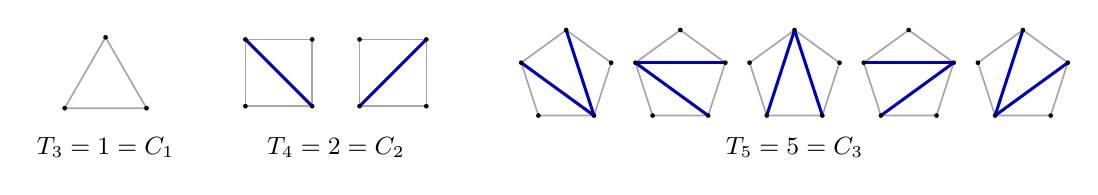
\begin{tikzpicture}
\draw[gray!70,line width=0.6pt,line join=round] (-0.52,-0.45) -- (0,0.45) -- (0.52,-0.45) -- cycle;
\fill[black] (-0.52,-0.45) circle (0.03);
\fill[black] (0,0.45) circle (0.03);
\fill[black] (0.52,-0.45) circle (0.03);
\node[font=\small] at (0,-0.95) {$T_3=1=C_1$};
\draw[gray!70,line width=0.6pt,line join=round] (1.776,-0.424) -- (1.776,0.424) -- (2.624,0.424) -- (2.624,-0.424) -- cycle;
\draw[cA,line width=1.1pt,line cap=round] (1.776,0.424) -- (2.624,-0.424);
\fill[black] (1.776,-0.424) circle (0.03);
\fill[black] (1.776,0.424) circle (0.03);
\fill[black] (2.624,0.424) circle (0.03);
\fill[black] (2.624,-0.424) circle (0.03);
\draw[gray!70,line width=0.6pt,line join=round] (3.226,-0.424) -- (3.226,0.424) -- (4.074,0.424) -- (4.074,-0.424) -- cycle;
\draw[cA,line width=1.1pt,line cap=round] (3.226,-0.424) -- (4.074,0.424);
\fill[black] (3.226,-0.424) circle (0.03);
\fill[black] (3.226,0.424) circle (0.03);
\fill[black] (4.074,0.424) circle (0.03);
\fill[black] (4.074,-0.424) circle (0.03);
\node[font=\small] at (2.925,-0.95) {$T_4=2=C_2$};
\draw[gray!70,line width=0.6pt,line join=round] (5.497,-0.543) -- (5.279,0.128) -- (5.85,0.543) -- (6.421,0.128) -- (6.203,-0.543) -- cycle;
\draw[cA,line width=1.1pt,line cap=round] (5.279,0.128) -- (6.203,-0.543);
\draw[cA,line width=1.1pt,line cap=round] (5.85,0.543) -- (6.203,-0.543);
\fill[black] (5.497,-0.543) circle (0.03);
\fill[black] (5.279,0.128) circle (0.03);
\fill[black] (5.85,0.543) circle (0.03);
\fill[black] (6.421,0.128) circle (0.03);
\fill[black] (6.203,-0.543) circle (0.03);
\draw[gray!70,line width=0.6pt,line join=round] (6.947,-0.543) -- (6.729,0.128) -- (7.3,0.543) -- (7.871,0.128) -- (7.653,-0.543) -- cycle;
\draw[cA,line width=1.1pt,line cap=round] (6.729,0.128) -- (7.871,0.128);
\draw[cA,line width=1.1pt,line cap=round] (6.729,0.128) -- (7.653,-0.543);
\fill[black] (6.947,-0.543) circle (0.03);
\fill[black] (6.729,0.128) circle (0.03);
\fill[black] (7.3,0.543) circle (0.03);
\fill[black] (7.871,0.128) circle (0.03);
\fill[black] (7.653,-0.543) circle (0.03);
\draw[gray!70,line width=0.6pt,line join=round] (8.397,-0.543) -- (8.179,0.128) -- (8.75,0.543) -- (9.321,0.128) -- (9.103,-0.543) -- cycle;
\draw[cA,line width=1.1pt,line cap=round] (8.397,-0.543) -- (8.75,0.543);
\draw[cA,line width=1.1pt,line cap=round] (8.75,0.543) -- (9.103,-0.543);
\fill[black] (8.397,-0.543) circle (0.03);
\fill[black] (8.179,0.128) circle (0.03);
\fill[black] (8.75,0.543) circle (0.03);
\fill[black] (9.321,0.128) circle (0.03);
\fill[black] (9.103,-0.543) circle (0.03);
\draw[gray!70,line width=0.6pt,line join=round] (9.847,-0.543) -- (9.629,0.128) -- (10.2,0.543) -- (10.771,0.128) -- (10.553,-0.543) -- cycle;
\draw[cA,line width=1.1pt,line cap=round] (9.847,-0.543) -- (10.771,0.128);
\draw[cA,line width=1.1pt,line cap=round] (9.629,0.128) -- (10.771,0.128);
\fill[black] (9.847,-0.543) circle (0.03);
\fill[black] (9.629,0.128) circle (0.03);
\fill[black] (10.2,0.543) circle (0.03);
\fill[black] (10.771,0.128) circle (0.03);
\fill[black] (10.553,-0.543) circle (0.03);
\draw[gray!70,line width=0.6pt,line join=round] (11.297,-0.543) -- (11.079,0.128) -- (11.65,0.543) -- (12.221,0.128) -- (12.003,-0.543) -- cycle;
\draw[cA,line width=1.1pt,line cap=round] (11.297,-0.543) -- (11.65,0.543);
\draw[cA,line width=1.1pt,line cap=round] (11.297,-0.543) -- (12.221,0.128);
\fill[black] (11.297,-0.543) circle (0.03);
\fill[black] (11.079,0.128) circle (0.03);
\fill[black] (11.65,0.543) circle (0.03);
\fill[black] (12.221,0.128) circle (0.03);
\fill[black] (12.003,-0.543) circle (0.03);
\node[font=\small] at (8.75,-0.95) {$T_5=5=C_3$};
\end{tikzpicture}}

\newcommand{\FigTriSplit}{%
\begin{tikzpicture}
\fill[cLeft!22] (-0.675,-1.169) -- (-1.35,0) -- (-0.675,1.169) -- cycle;
\fill[cRight!20] (-0.675,1.169) -- (0.675,1.169) -- (1.35,0) -- (0.675,-1.169) -- cycle;
\fill[cTop!38] (-0.675,-1.169) -- (-0.675,1.169) -- (0.675,-1.169) -- cycle;
\draw[gray!70,line width=0.7pt,line join=round] (-0.675,-1.169) -- (-1.35,0) -- (-0.675,1.169) -- (0.675,1.169) -- (1.35,0) -- (0.675,-1.169) -- cycle;
\draw[cTop,line width=1.3pt,line cap=round] (-0.675,-1.169) -- (-0.675,1.169) -- (0.675,-1.169);
\draw[cTop,line width=2.2pt,line cap=round] (-0.675,-1.169) -- (0.675,-1.169);
\fill (-0.675,-1.169) circle (0.045);
\node[font=\small] at (-0.825,-1.429) {$0$};
\fill (-1.35,0) circle (0.045);
\node[font=\small] at (-1.65,0) {$1$};
\fill (-0.675,1.169) circle (0.045);
\node[font=\small] at (-0.825,1.429) {$2$};
\fill (0.675,1.169) circle (0.045);
\node[font=\small] at (0.825,1.429) {$3$};
\fill (1.35,0) circle (0.045);
\node[font=\small] at (1.65,0) {$4$};
\fill (0.675,-1.169) circle (0.045);
\node[font=\small] at (0.825,-1.429) {$5$};
\node[font=\small,text=cTop!80!black] at (-0.225,-0.39) {根};
\node[font=\small,text=cLeft!80!black,align=center] at (-0.9,0) {左\\$C_1$};
\node[font=\small,text=cRight!85!black,align=center] at (0.506,0.292) {右\\$C_2$};
\node[font=\small,text=cTop!80!black] at (0,-1.489) {底邊};
\end{tikzpicture}}

\newcommand{\FigTriGroups}{%
\begin{tikzpicture}
\fill[cTop!38] (-4.575,-0.45) -- (-4.835,0) -- (-4.055,-0.45) -- cycle;
\fill[cRight!20] (-4.835,0) -- (-4.575,0.45) -- (-4.055,0.45) -- (-3.795,0) -- (-4.055,-0.45) -- cycle;
\draw[gray!70,line width=0.6pt,line join=round] (-4.575,-0.45) -- (-4.835,0) -- (-4.575,0.45) -- (-4.055,0.45) -- (-3.795,0) -- (-4.055,-0.45) -- cycle;
\draw[cTop,line width=1.1pt,line cap=round] (-4.835,0) -- (-4.055,-0.45);
\draw[cRight,line width=1.1pt,line cap=round] (-4.575,0.45) -- (-4.055,-0.45);
\draw[cRight,line width=1.1pt,line cap=round] (-4.055,0.45) -- (-4.055,-0.45);
\fill[black] (-4.575,-0.45) circle (0.03);
\fill[black] (-4.835,0) circle (0.03);
\fill[black] (-4.575,0.45) circle (0.03);
\fill[black] (-4.055,0.45) circle (0.03);
\fill[black] (-3.795,0) circle (0.03);
\fill[black] (-4.055,-0.45) circle (0.03);
\fill[cTop!38] (-3.295,-0.45) -- (-3.555,0) -- (-2.775,-0.45) -- cycle;
\fill[cRight!20] (-3.555,0) -- (-3.295,0.45) -- (-2.775,0.45) -- (-2.515,0) -- (-2.775,-0.45) -- cycle;
\draw[gray!70,line width=0.6pt,line join=round] (-3.295,-0.45) -- (-3.555,0) -- (-3.295,0.45) -- (-2.775,0.45) -- (-2.515,0) -- (-2.775,-0.45) -- cycle;
\draw[cTop,line width=1.1pt,line cap=round] (-3.555,0) -- (-2.775,-0.45);
\draw[cRight,line width=1.1pt,line cap=round] (-3.295,0.45) -- (-2.775,-0.45);
\draw[cRight,line width=1.1pt,line cap=round] (-3.295,0.45) -- (-2.515,0);
\fill[black] (-3.295,-0.45) circle (0.03);
\fill[black] (-3.555,0) circle (0.03);
\fill[black] (-3.295,0.45) circle (0.03);
\fill[black] (-2.775,0.45) circle (0.03);
\fill[black] (-2.515,0) circle (0.03);
\fill[black] (-2.775,-0.45) circle (0.03);
\fill[cTop!38] (-2.015,-0.45) -- (-2.275,0) -- (-1.495,-0.45) -- cycle;
\fill[cRight!20] (-2.275,0) -- (-2.015,0.45) -- (-1.495,0.45) -- (-1.235,0) -- (-1.495,-0.45) -- cycle;
\draw[gray!70,line width=0.6pt,line join=round] (-2.015,-0.45) -- (-2.275,0) -- (-2.015,0.45) -- (-1.495,0.45) -- (-1.235,0) -- (-1.495,-0.45) -- cycle;
\draw[cTop,line width=1.1pt,line cap=round] (-2.275,0) -- (-1.495,-0.45);
\draw[cRight,line width=1.1pt,line cap=round] (-2.275,0) -- (-1.495,0.45);
\draw[cRight,line width=1.1pt,line cap=round] (-1.495,0.45) -- (-1.495,-0.45);
\fill[black] (-2.015,-0.45) circle (0.03);
\fill[black] (-2.275,0) circle (0.03);
\fill[black] (-2.015,0.45) circle (0.03);
\fill[black] (-1.495,0.45) circle (0.03);
\fill[black] (-1.235,0) circle (0.03);
\fill[black] (-1.495,-0.45) circle (0.03);
\fill[cTop!38] (-0.735,-0.45) -- (-0.995,0) -- (-0.215,-0.45) -- cycle;
\fill[cRight!20] (-0.995,0) -- (-0.735,0.45) -- (-0.215,0.45) -- (0.045,0) -- (-0.215,-0.45) -- cycle;
\draw[gray!70,line width=0.6pt,line join=round] (-0.735,-0.45) -- (-0.995,0) -- (-0.735,0.45) -- (-0.215,0.45) -- (0.045,0) -- (-0.215,-0.45) -- cycle;
\draw[cTop,line width=1.1pt,line cap=round] (-0.995,0) -- (-0.215,-0.45);
\draw[cRight,line width=1.1pt,line cap=round] (-0.995,0) -- (0.045,0);
\draw[cRight,line width=1.1pt,line cap=round] (-0.735,0.45) -- (0.045,0);
\fill[black] (-0.735,-0.45) circle (0.03);
\fill[black] (-0.995,0) circle (0.03);
\fill[black] (-0.735,0.45) circle (0.03);
\fill[black] (-0.215,0.45) circle (0.03);
\fill[black] (0.045,0) circle (0.03);
\fill[black] (-0.215,-0.45) circle (0.03);
\fill[cTop!38] (0.545,-0.45) -- (0.285,0) -- (1.065,-0.45) -- cycle;
\fill[cRight!20] (0.285,0) -- (0.545,0.45) -- (1.065,0.45) -- (1.325,0) -- (1.065,-0.45) -- cycle;
\draw[gray!70,line width=0.6pt,line join=round] (0.545,-0.45) -- (0.285,0) -- (0.545,0.45) -- (1.065,0.45) -- (1.325,0) -- (1.065,-0.45) -- cycle;
\draw[cTop,line width=1.1pt,line cap=round] (0.285,0) -- (1.065,-0.45);
\draw[cRight,line width=1.1pt,line cap=round] (0.285,0) -- (1.325,0);
\draw[cRight,line width=1.1pt,line cap=round] (0.285,0) -- (1.065,0.45);
\fill[black] (0.545,-0.45) circle (0.03);
\fill[black] (0.285,0) circle (0.03);
\fill[black] (0.545,0.45) circle (0.03);
\fill[black] (1.065,0.45) circle (0.03);
\fill[black] (1.325,0) circle (0.03);
\fill[black] (1.065,-0.45) circle (0.03);
\node[font=\footnotesize] at (-1.755,-0.82) {$k=1$：$\textcolor{cLeft}{C_0}\textcolor{cRight}{C_3}=1\cdot5=5$};
\fill[cTop!38] (2.775,-0.45) -- (2.775,0.45) -- (3.295,-0.45) -- cycle;
\fill[cLeft!22] (2.775,-0.45) -- (2.515,0) -- (2.775,0.45) -- cycle;
\fill[cRight!20] (2.775,0.45) -- (3.295,0.45) -- (3.555,0) -- (3.295,-0.45) -- cycle;
\draw[gray!70,line width=0.6pt,line join=round] (2.775,-0.45) -- (2.515,0) -- (2.775,0.45) -- (3.295,0.45) -- (3.555,0) -- (3.295,-0.45) -- cycle;
\draw[cTop,line width=1.1pt,line cap=round] (2.775,-0.45) -- (2.775,0.45);
\draw[cTop,line width=1.1pt,line cap=round] (2.775,0.45) -- (3.295,-0.45);
\draw[cRight,line width=1.1pt,line cap=round] (3.295,0.45) -- (3.295,-0.45);
\fill[black] (2.775,-0.45) circle (0.03);
\fill[black] (2.515,0) circle (0.03);
\fill[black] (2.775,0.45) circle (0.03);
\fill[black] (3.295,0.45) circle (0.03);
\fill[black] (3.555,0) circle (0.03);
\fill[black] (3.295,-0.45) circle (0.03);
\fill[cTop!38] (4.055,-0.45) -- (4.055,0.45) -- (4.575,-0.45) -- cycle;
\fill[cLeft!22] (4.055,-0.45) -- (3.795,0) -- (4.055,0.45) -- cycle;
\fill[cRight!20] (4.055,0.45) -- (4.575,0.45) -- (4.835,0) -- (4.575,-0.45) -- cycle;
\draw[gray!70,line width=0.6pt,line join=round] (4.055,-0.45) -- (3.795,0) -- (4.055,0.45) -- (4.575,0.45) -- (4.835,0) -- (4.575,-0.45) -- cycle;
\draw[cTop,line width=1.1pt,line cap=round] (4.055,-0.45) -- (4.055,0.45);
\draw[cTop,line width=1.1pt,line cap=round] (4.055,0.45) -- (4.575,-0.45);
\draw[cRight,line width=1.1pt,line cap=round] (4.055,0.45) -- (4.835,0);
\fill[black] (4.055,-0.45) circle (0.03);
\fill[black] (3.795,0) circle (0.03);
\fill[black] (4.055,0.45) circle (0.03);
\fill[black] (4.575,0.45) circle (0.03);
\fill[black] (4.835,0) circle (0.03);
\fill[black] (4.575,-0.45) circle (0.03);
\node[font=\footnotesize] at (3.675,-0.82) {$k=2$：$\textcolor{cLeft}{C_1}\textcolor{cRight}{C_2}=1\cdot2=2$};
\fill[cTop!38] (-4.575,-2.5) -- (-4.055,-1.6) -- (-4.055,-2.5) -- cycle;
\fill[cLeft!22] (-4.575,-2.5) -- (-4.835,-2.05) -- (-4.575,-1.6) -- (-4.055,-1.6) -- cycle;
\fill[cRight!20] (-4.055,-1.6) -- (-3.795,-2.05) -- (-4.055,-2.5) -- cycle;
\draw[gray!70,line width=0.6pt,line join=round] (-4.575,-2.5) -- (-4.835,-2.05) -- (-4.575,-1.6) -- (-4.055,-1.6) -- (-3.795,-2.05) -- (-4.055,-2.5) -- cycle;
\draw[cTop,line width=1.1pt,line cap=round] (-4.575,-2.5) -- (-4.055,-1.6);
\draw[cTop,line width=1.1pt,line cap=round] (-4.055,-1.6) -- (-4.055,-2.5);
\draw[cLeft,line width=1.1pt,line cap=round] (-4.835,-2.05) -- (-4.055,-1.6);
\fill[black] (-4.575,-2.5) circle (0.03);
\fill[black] (-4.835,-2.05) circle (0.03);
\fill[black] (-4.575,-1.6) circle (0.03);
\fill[black] (-4.055,-1.6) circle (0.03);
\fill[black] (-3.795,-2.05) circle (0.03);
\fill[black] (-4.055,-2.5) circle (0.03);
\fill[cTop!38] (-3.295,-2.5) -- (-2.775,-1.6) -- (-2.775,-2.5) -- cycle;
\fill[cLeft!22] (-3.295,-2.5) -- (-3.555,-2.05) -- (-3.295,-1.6) -- (-2.775,-1.6) -- cycle;
\fill[cRight!20] (-2.775,-1.6) -- (-2.515,-2.05) -- (-2.775,-2.5) -- cycle;
\draw[gray!70,line width=0.6pt,line join=round] (-3.295,-2.5) -- (-3.555,-2.05) -- (-3.295,-1.6) -- (-2.775,-1.6) -- (-2.515,-2.05) -- (-2.775,-2.5) -- cycle;
\draw[cTop,line width=1.1pt,line cap=round] (-3.295,-2.5) -- (-2.775,-1.6);
\draw[cTop,line width=1.1pt,line cap=round] (-2.775,-1.6) -- (-2.775,-2.5);
\draw[cLeft,line width=1.1pt,line cap=round] (-3.295,-2.5) -- (-3.295,-1.6);
\fill[black] (-3.295,-2.5) circle (0.03);
\fill[black] (-3.555,-2.05) circle (0.03);
\fill[black] (-3.295,-1.6) circle (0.03);
\fill[black] (-2.775,-1.6) circle (0.03);
\fill[black] (-2.515,-2.05) circle (0.03);
\fill[black] (-2.775,-2.5) circle (0.03);
\node[font=\footnotesize] at (-3.675,-2.87) {$k=3$：$\textcolor{cLeft}{C_2}\textcolor{cRight}{C_1}=2\cdot1=2$};
\fill[cTop!38] (-1.065,-2.5) -- (-0.285,-2.05) -- (-0.545,-2.5) -- cycle;
\fill[cLeft!22] (-1.065,-2.5) -- (-1.325,-2.05) -- (-1.065,-1.6) -- (-0.545,-1.6) -- (-0.285,-2.05) -- cycle;
\draw[gray!70,line width=0.6pt,line join=round] (-1.065,-2.5) -- (-1.325,-2.05) -- (-1.065,-1.6) -- (-0.545,-1.6) -- (-0.285,-2.05) -- (-0.545,-2.5) -- cycle;
\draw[cTop,line width=1.1pt,line cap=round] (-1.065,-2.5) -- (-0.285,-2.05);
\draw[cLeft,line width=1.1pt,line cap=round] (-1.325,-2.05) -- (-0.285,-2.05);
\draw[cLeft,line width=1.1pt,line cap=round] (-1.065,-1.6) -- (-0.285,-2.05);
\fill[black] (-1.065,-2.5) circle (0.03);
\fill[black] (-1.325,-2.05) circle (0.03);
\fill[black] (-1.065,-1.6) circle (0.03);
\fill[black] (-0.545,-1.6) circle (0.03);
\fill[black] (-0.285,-2.05) circle (0.03);
\fill[black] (-0.545,-2.5) circle (0.03);
\fill[cTop!38] (0.215,-2.5) -- (0.995,-2.05) -- (0.735,-2.5) -- cycle;
\fill[cLeft!22] (0.215,-2.5) -- (-0.045,-2.05) -- (0.215,-1.6) -- (0.735,-1.6) -- (0.995,-2.05) -- cycle;
\draw[gray!70,line width=0.6pt,line join=round] (0.215,-2.5) -- (-0.045,-2.05) -- (0.215,-1.6) -- (0.735,-1.6) -- (0.995,-2.05) -- (0.735,-2.5) -- cycle;
\draw[cTop,line width=1.1pt,line cap=round] (0.215,-2.5) -- (0.995,-2.05);
\draw[cLeft,line width=1.1pt,line cap=round] (-0.045,-2.05) -- (0.995,-2.05);
\draw[cLeft,line width=1.1pt,line cap=round] (-0.045,-2.05) -- (0.735,-1.6);
\fill[black] (0.215,-2.5) circle (0.03);
\fill[black] (-0.045,-2.05) circle (0.03);
\fill[black] (0.215,-1.6) circle (0.03);
\fill[black] (0.735,-1.6) circle (0.03);
\fill[black] (0.995,-2.05) circle (0.03);
\fill[black] (0.735,-2.5) circle (0.03);
\fill[cTop!38] (1.495,-2.5) -- (2.275,-2.05) -- (2.015,-2.5) -- cycle;
\fill[cLeft!22] (1.495,-2.5) -- (1.235,-2.05) -- (1.495,-1.6) -- (2.015,-1.6) -- (2.275,-2.05) -- cycle;
\draw[gray!70,line width=0.6pt,line join=round] (1.495,-2.5) -- (1.235,-2.05) -- (1.495,-1.6) -- (2.015,-1.6) -- (2.275,-2.05) -- (2.015,-2.5) -- cycle;
\draw[cTop,line width=1.1pt,line cap=round] (1.495,-2.5) -- (2.275,-2.05);
\draw[cLeft,line width=1.1pt,line cap=round] (1.495,-2.5) -- (1.495,-1.6);
\draw[cLeft,line width=1.1pt,line cap=round] (1.495,-1.6) -- (2.275,-2.05);
\fill[black] (1.495,-2.5) circle (0.03);
\fill[black] (1.235,-2.05) circle (0.03);
\fill[black] (1.495,-1.6) circle (0.03);
\fill[black] (2.015,-1.6) circle (0.03);
\fill[black] (2.275,-2.05) circle (0.03);
\fill[black] (2.015,-2.5) circle (0.03);
\fill[cTop!38] (2.775,-2.5) -- (3.555,-2.05) -- (3.295,-2.5) -- cycle;
\fill[cLeft!22] (2.775,-2.5) -- (2.515,-2.05) -- (2.775,-1.6) -- (3.295,-1.6) -- (3.555,-2.05) -- cycle;
\draw[gray!70,line width=0.6pt,line join=round] (2.775,-2.5) -- (2.515,-2.05) -- (2.775,-1.6) -- (3.295,-1.6) -- (3.555,-2.05) -- (3.295,-2.5) -- cycle;
\draw[cTop,line width=1.1pt,line cap=round] (2.775,-2.5) -- (3.555,-2.05);
\draw[cLeft,line width=1.1pt,line cap=round] (2.775,-2.5) -- (3.295,-1.6);
\draw[cLeft,line width=1.1pt,line cap=round] (2.515,-2.05) -- (3.295,-1.6);
\fill[black] (2.775,-2.5) circle (0.03);
\fill[black] (2.515,-2.05) circle (0.03);
\fill[black] (2.775,-1.6) circle (0.03);
\fill[black] (3.295,-1.6) circle (0.03);
\fill[black] (3.555,-2.05) circle (0.03);
\fill[black] (3.295,-2.5) circle (0.03);
\fill[cTop!38] (4.055,-2.5) -- (4.835,-2.05) -- (4.575,-2.5) -- cycle;
\fill[cLeft!22] (4.055,-2.5) -- (3.795,-2.05) -- (4.055,-1.6) -- (4.575,-1.6) -- (4.835,-2.05) -- cycle;
\draw[gray!70,line width=0.6pt,line join=round] (4.055,-2.5) -- (3.795,-2.05) -- (4.055,-1.6) -- (4.575,-1.6) -- (4.835,-2.05) -- (4.575,-2.5) -- cycle;
\draw[cTop,line width=1.1pt,line cap=round] (4.055,-2.5) -- (4.835,-2.05);
\draw[cLeft,line width=1.1pt,line cap=round] (4.055,-2.5) -- (4.575,-1.6);
\draw[cLeft,line width=1.1pt,line cap=round] (4.055,-2.5) -- (4.055,-1.6);
\fill[black] (4.055,-2.5) circle (0.03);
\fill[black] (3.795,-2.05) circle (0.03);
\fill[black] (4.055,-1.6) circle (0.03);
\fill[black] (4.575,-1.6) circle (0.03);
\fill[black] (4.835,-2.05) circle (0.03);
\fill[black] (4.575,-2.5) circle (0.03);
\node[font=\footnotesize] at (1.755,-2.87) {$k=4$：$\textcolor{cLeft}{C_3}\textcolor{cRight}{C_0}=5\cdot1=5$};
\end{tikzpicture}}

\newcommand{\FigParenTrees}{%
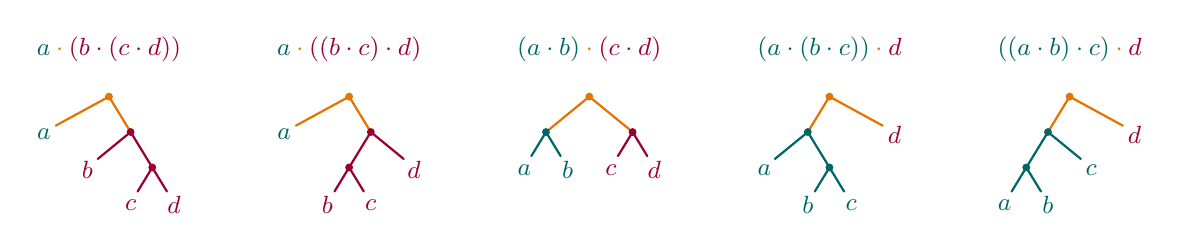
\begin{tikzpicture}
\node[font=\small] at (0,0) {${\color{cLeft}a}\mathbin{\color{cTop}\cdot}{\color{cRight}(b\cdot (c\cdot d))}$};
\draw[cTop,line width=0.8pt,line cap=round] (0,-0.6) -- (-0.676,-0.969);
\draw[cTop,line width=0.8pt,line cap=round] (0,-0.6) -- (0.275,-1.05);
\draw[cRight,line width=0.8pt,line cap=round] (0.275,-1.05) -- (-0.143,-1.392);
\draw[cRight,line width=0.8pt,line cap=round] (0.275,-1.05) -- (0.55,-1.5);
\draw[cRight,line width=0.8pt,line cap=round] (0.55,-1.5) -- (0.364,-1.805);
\draw[cRight,line width=0.8pt,line cap=round] (0.55,-1.5) -- (0.736,-1.805);
\fill[cTop] (0,-0.6) circle (0.05);
\fill[cRight] (0.275,-1.05) circle (0.05);
\fill[cRight] (0.55,-1.5) circle (0.05);
\node[font=\small,inner sep=0pt,text=cLeft] at (-0.825,-1.08) {$a$};
\node[font=\small,inner sep=0pt,text=cRight] at (-0.275,-1.53) {$b$};
\node[font=\small,inner sep=0pt,text=cRight] at (0.275,-1.98) {$c$};
\node[font=\small,inner sep=0pt,text=cRight] at (0.825,-1.98) {$d$};
\node[font=\small] at (3.05,0) {${\color{cLeft}a}\mathbin{\color{cTop}\cdot}{\color{cRight}((b\cdot c)\cdot d)}$};
\draw[cTop,line width=0.8pt,line cap=round] (3.05,-0.6) -- (2.374,-0.969);
\draw[cTop,line width=0.8pt,line cap=round] (3.05,-0.6) -- (3.325,-1.05);
\draw[cRight,line width=0.8pt,line cap=round] (3.05,-1.5) -- (2.864,-1.805);
\draw[cRight,line width=0.8pt,line cap=round] (3.05,-1.5) -- (3.236,-1.805);
\draw[cRight,line width=0.8pt,line cap=round] (3.325,-1.05) -- (3.05,-1.5);
\draw[cRight,line width=0.8pt,line cap=round] (3.325,-1.05) -- (3.743,-1.392);
\fill[cTop] (3.05,-0.6) circle (0.05);
\fill[cRight] (3.05,-1.5) circle (0.05);
\fill[cRight] (3.325,-1.05) circle (0.05);
\node[font=\small,inner sep=0pt,text=cLeft] at (2.225,-1.08) {$a$};
\node[font=\small,inner sep=0pt,text=cRight] at (2.775,-1.98) {$b$};
\node[font=\small,inner sep=0pt,text=cRight] at (3.325,-1.98) {$c$};
\node[font=\small,inner sep=0pt,text=cRight] at (3.875,-1.53) {$d$};
\node[font=\small] at (6.1,0) {${\color{cLeft}(a\cdot b)}\mathbin{\color{cTop}\cdot}{\color{cRight}(c\cdot d)}$};
\draw[cLeft,line width=0.8pt,line cap=round] (5.55,-1.05) -- (5.364,-1.355);
\draw[cLeft,line width=0.8pt,line cap=round] (5.55,-1.05) -- (5.736,-1.355);
\draw[cTop,line width=0.8pt,line cap=round] (6.1,-0.6) -- (5.55,-1.05);
\draw[cTop,line width=0.8pt,line cap=round] (6.1,-0.6) -- (6.65,-1.05);
\draw[cRight,line width=0.8pt,line cap=round] (6.65,-1.05) -- (6.464,-1.355);
\draw[cRight,line width=0.8pt,line cap=round] (6.65,-1.05) -- (6.836,-1.355);
\fill[cLeft] (5.55,-1.05) circle (0.05);
\fill[cTop] (6.1,-0.6) circle (0.05);
\fill[cRight] (6.65,-1.05) circle (0.05);
\node[font=\small,inner sep=0pt,text=cLeft] at (5.275,-1.53) {$a$};
\node[font=\small,inner sep=0pt,text=cLeft] at (5.825,-1.53) {$b$};
\node[font=\small,inner sep=0pt,text=cRight] at (6.375,-1.53) {$c$};
\node[font=\small,inner sep=0pt,text=cRight] at (6.925,-1.53) {$d$};
\node[font=\small] at (9.15,0) {${\color{cLeft}(a\cdot (b\cdot c))}\mathbin{\color{cTop}\cdot}{\color{cRight}d}$};
\draw[cLeft,line width=0.8pt,line cap=round] (8.875,-1.05) -- (8.457,-1.392);
\draw[cLeft,line width=0.8pt,line cap=round] (8.875,-1.05) -- (9.15,-1.5);
\draw[cLeft,line width=0.8pt,line cap=round] (9.15,-1.5) -- (8.964,-1.805);
\draw[cLeft,line width=0.8pt,line cap=round] (9.15,-1.5) -- (9.336,-1.805);
\draw[cTop,line width=0.8pt,line cap=round] (9.15,-0.6) -- (8.875,-1.05);
\draw[cTop,line width=0.8pt,line cap=round] (9.15,-0.6) -- (9.826,-0.969);
\fill[cLeft] (8.875,-1.05) circle (0.05);
\fill[cLeft] (9.15,-1.5) circle (0.05);
\fill[cTop] (9.15,-0.6) circle (0.05);
\node[font=\small,inner sep=0pt,text=cLeft] at (8.325,-1.53) {$a$};
\node[font=\small,inner sep=0pt,text=cLeft] at (8.875,-1.98) {$b$};
\node[font=\small,inner sep=0pt,text=cLeft] at (9.425,-1.98) {$c$};
\node[font=\small,inner sep=0pt,text=cRight] at (9.975,-1.08) {$d$};
\node[font=\small] at (12.2,0) {${\color{cLeft}((a\cdot b)\cdot c)}\mathbin{\color{cTop}\cdot}{\color{cRight}d}$};
\draw[cLeft,line width=0.8pt,line cap=round] (11.65,-1.5) -- (11.464,-1.805);
\draw[cLeft,line width=0.8pt,line cap=round] (11.65,-1.5) -- (11.836,-1.805);
\draw[cLeft,line width=0.8pt,line cap=round] (11.925,-1.05) -- (11.65,-1.5);
\draw[cLeft,line width=0.8pt,line cap=round] (11.925,-1.05) -- (12.343,-1.392);
\draw[cTop,line width=0.8pt,line cap=round] (12.2,-0.6) -- (11.925,-1.05);
\draw[cTop,line width=0.8pt,line cap=round] (12.2,-0.6) -- (12.876,-0.969);
\fill[cLeft] (11.65,-1.5) circle (0.05);
\fill[cLeft] (11.925,-1.05) circle (0.05);
\fill[cTop] (12.2,-0.6) circle (0.05);
\node[font=\small,inner sep=0pt,text=cLeft] at (11.375,-1.98) {$a$};
\node[font=\small,inner sep=0pt,text=cLeft] at (11.925,-1.98) {$b$};
\node[font=\small,inner sep=0pt,text=cLeft] at (12.475,-1.53) {$c$};
\node[font=\small,inner sep=0pt,text=cRight] at (13.025,-1.08) {$d$};
\end{tikzpicture}}

\newcommand{\FigLatticeAll}{%
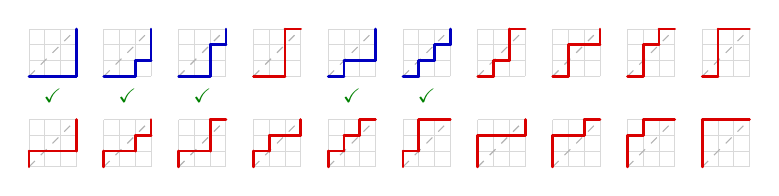
\begin{tikzpicture}
\draw[gray!30,line width=0.3pt] (0,0) -- (0,0.6);
\draw[gray!30,line width=0.3pt] (0.2,0) -- (0.2,0.6);
\draw[gray!30,line width=0.3pt] (0.4,0) -- (0.4,0.6);
\draw[gray!30,line width=0.3pt] (0.6,0) -- (0.6,0.6);
\draw[gray!30,line width=0.3pt] (0,0) -- (0.6,0);
\draw[gray!30,line width=0.3pt] (0,0.2) -- (0.6,0.2);
\draw[gray!30,line width=0.3pt] (0,0.4) -- (0.6,0.4);
\draw[gray!30,line width=0.3pt] (0,0.6) -- (0.6,0.6);
\draw[gray!60,dashed,line width=0.4pt] (0,0) -- (0.6,0.6);
\draw[cA,line width=1.0pt,line cap=round] (0,0) -- (0.2,0);
\draw[cA,line width=1.0pt,line cap=round] (0.2,0) -- (0.4,0);
\draw[cA,line width=1.0pt,line cap=round] (0.4,0) -- (0.6,0);
\draw[cA,line width=1.0pt,line cap=round] (0.6,0) -- (0.6,0.2);
\draw[cA,line width=1.0pt,line cap=round] (0.6,0.2) -- (0.6,0.4);
\draw[cA,line width=1.0pt,line cap=round] (0.6,0.4) -- (0.6,0.6);
\node[font=\scriptsize,text=green!50!black] at (0.3,-0.25) {\checkmark};
\draw[gray!30,line width=0.3pt] (0.95,0) -- (0.95,0.6);
\draw[gray!30,line width=0.3pt] (1.15,0) -- (1.15,0.6);
\draw[gray!30,line width=0.3pt] (1.35,0) -- (1.35,0.6);
\draw[gray!30,line width=0.3pt] (1.55,0) -- (1.55,0.6);
\draw[gray!30,line width=0.3pt] (0.95,0) -- (1.55,0);
\draw[gray!30,line width=0.3pt] (0.95,0.2) -- (1.55,0.2);
\draw[gray!30,line width=0.3pt] (0.95,0.4) -- (1.55,0.4);
\draw[gray!30,line width=0.3pt] (0.95,0.6) -- (1.55,0.6);
\draw[gray!60,dashed,line width=0.4pt] (0.95,0) -- (1.55,0.6);
\draw[cA,line width=1.0pt,line cap=round] (0.95,0) -- (1.15,0);
\draw[cA,line width=1.0pt,line cap=round] (1.15,0) -- (1.35,0);
\draw[cA,line width=1.0pt,line cap=round] (1.35,0) -- (1.35,0.2);
\draw[cA,line width=1.0pt,line cap=round] (1.35,0.2) -- (1.55,0.2);
\draw[cA,line width=1.0pt,line cap=round] (1.55,0.2) -- (1.55,0.4);
\draw[cA,line width=1.0pt,line cap=round] (1.55,0.4) -- (1.55,0.6);
\node[font=\scriptsize,text=green!50!black] at (1.25,-0.25) {\checkmark};
\draw[gray!30,line width=0.3pt] (1.9,0) -- (1.9,0.6);
\draw[gray!30,line width=0.3pt] (2.1,0) -- (2.1,0.6);
\draw[gray!30,line width=0.3pt] (2.3,0) -- (2.3,0.6);
\draw[gray!30,line width=0.3pt] (2.5,0) -- (2.5,0.6);
\draw[gray!30,line width=0.3pt] (1.9,0) -- (2.5,0);
\draw[gray!30,line width=0.3pt] (1.9,0.2) -- (2.5,0.2);
\draw[gray!30,line width=0.3pt] (1.9,0.4) -- (2.5,0.4);
\draw[gray!30,line width=0.3pt] (1.9,0.6) -- (2.5,0.6);
\draw[gray!60,dashed,line width=0.4pt] (1.9,0) -- (2.5,0.6);
\draw[cA,line width=1.0pt,line cap=round] (1.9,0) -- (2.1,0);
\draw[cA,line width=1.0pt,line cap=round] (2.1,0) -- (2.3,0);
\draw[cA,line width=1.0pt,line cap=round] (2.3,0) -- (2.3,0.2);
\draw[cA,line width=1.0pt,line cap=round] (2.3,0.2) -- (2.3,0.4);
\draw[cA,line width=1.0pt,line cap=round] (2.3,0.4) -- (2.5,0.4);
\draw[cA,line width=1.0pt,line cap=round] (2.5,0.4) -- (2.5,0.6);
\node[font=\scriptsize,text=green!50!black] at (2.2,-0.25) {\checkmark};
\draw[gray!30,line width=0.3pt] (2.85,0) -- (2.85,0.6);
\draw[gray!30,line width=0.3pt] (3.05,0) -- (3.05,0.6);
\draw[gray!30,line width=0.3pt] (3.25,0) -- (3.25,0.6);
\draw[gray!30,line width=0.3pt] (3.45,0) -- (3.45,0.6);
\draw[gray!30,line width=0.3pt] (2.85,0) -- (3.45,0);
\draw[gray!30,line width=0.3pt] (2.85,0.2) -- (3.45,0.2);
\draw[gray!30,line width=0.3pt] (2.85,0.4) -- (3.45,0.4);
\draw[gray!30,line width=0.3pt] (2.85,0.6) -- (3.45,0.6);
\draw[gray!60,dashed,line width=0.4pt] (2.85,0) -- (3.45,0.6);
\draw[cBad,line width=1.0pt,line cap=round] (2.85,0) -- (3.05,0);
\draw[cBad,line width=1.0pt,line cap=round] (3.05,0) -- (3.25,0);
\draw[cBad,line width=1.0pt,line cap=round] (3.25,0) -- (3.25,0.2);
\draw[cBad,line width=1.0pt,line cap=round] (3.25,0.2) -- (3.25,0.4);
\draw[cBad,line width=1.0pt,line cap=round] (3.25,0.4) -- (3.25,0.6);
\draw[cBad,line width=1.0pt,line cap=round] (3.25,0.6) -- (3.45,0.6);
\draw[gray!30,line width=0.3pt] (3.8,0) -- (3.8,0.6);
\draw[gray!30,line width=0.3pt] (4,0) -- (4,0.6);
\draw[gray!30,line width=0.3pt] (4.2,0) -- (4.2,0.6);
\draw[gray!30,line width=0.3pt] (4.4,0) -- (4.4,0.6);
\draw[gray!30,line width=0.3pt] (3.8,0) -- (4.4,0);
\draw[gray!30,line width=0.3pt] (3.8,0.2) -- (4.4,0.2);
\draw[gray!30,line width=0.3pt] (3.8,0.4) -- (4.4,0.4);
\draw[gray!30,line width=0.3pt] (3.8,0.6) -- (4.4,0.6);
\draw[gray!60,dashed,line width=0.4pt] (3.8,0) -- (4.4,0.6);
\draw[cA,line width=1.0pt,line cap=round] (3.8,0) -- (4,0);
\draw[cA,line width=1.0pt,line cap=round] (4,0) -- (4,0.2);
\draw[cA,line width=1.0pt,line cap=round] (4,0.2) -- (4.2,0.2);
\draw[cA,line width=1.0pt,line cap=round] (4.2,0.2) -- (4.4,0.2);
\draw[cA,line width=1.0pt,line cap=round] (4.4,0.2) -- (4.4,0.4);
\draw[cA,line width=1.0pt,line cap=round] (4.4,0.4) -- (4.4,0.6);
\node[font=\scriptsize,text=green!50!black] at (4.1,-0.25) {\checkmark};
\draw[gray!30,line width=0.3pt] (4.75,0) -- (4.75,0.6);
\draw[gray!30,line width=0.3pt] (4.95,0) -- (4.95,0.6);
\draw[gray!30,line width=0.3pt] (5.15,0) -- (5.15,0.6);
\draw[gray!30,line width=0.3pt] (5.35,0) -- (5.35,0.6);
\draw[gray!30,line width=0.3pt] (4.75,0) -- (5.35,0);
\draw[gray!30,line width=0.3pt] (4.75,0.2) -- (5.35,0.2);
\draw[gray!30,line width=0.3pt] (4.75,0.4) -- (5.35,0.4);
\draw[gray!30,line width=0.3pt] (4.75,0.6) -- (5.35,0.6);
\draw[gray!60,dashed,line width=0.4pt] (4.75,0) -- (5.35,0.6);
\draw[cA,line width=1.0pt,line cap=round] (4.75,0) -- (4.95,0);
\draw[cA,line width=1.0pt,line cap=round] (4.95,0) -- (4.95,0.2);
\draw[cA,line width=1.0pt,line cap=round] (4.95,0.2) -- (5.15,0.2);
\draw[cA,line width=1.0pt,line cap=round] (5.15,0.2) -- (5.15,0.4);
\draw[cA,line width=1.0pt,line cap=round] (5.15,0.4) -- (5.35,0.4);
\draw[cA,line width=1.0pt,line cap=round] (5.35,0.4) -- (5.35,0.6);
\node[font=\scriptsize,text=green!50!black] at (5.05,-0.25) {\checkmark};
\draw[gray!30,line width=0.3pt] (5.7,0) -- (5.7,0.6);
\draw[gray!30,line width=0.3pt] (5.9,0) -- (5.9,0.6);
\draw[gray!30,line width=0.3pt] (6.1,0) -- (6.1,0.6);
\draw[gray!30,line width=0.3pt] (6.3,0) -- (6.3,0.6);
\draw[gray!30,line width=0.3pt] (5.7,0) -- (6.3,0);
\draw[gray!30,line width=0.3pt] (5.7,0.2) -- (6.3,0.2);
\draw[gray!30,line width=0.3pt] (5.7,0.4) -- (6.3,0.4);
\draw[gray!30,line width=0.3pt] (5.7,0.6) -- (6.3,0.6);
\draw[gray!60,dashed,line width=0.4pt] (5.7,0) -- (6.3,0.6);
\draw[cBad,line width=1.0pt,line cap=round] (5.7,0) -- (5.9,0);
\draw[cBad,line width=1.0pt,line cap=round] (5.9,0) -- (5.9,0.2);
\draw[cBad,line width=1.0pt,line cap=round] (5.9,0.2) -- (6.1,0.2);
\draw[cBad,line width=1.0pt,line cap=round] (6.1,0.2) -- (6.1,0.4);
\draw[cBad,line width=1.0pt,line cap=round] (6.1,0.4) -- (6.1,0.6);
\draw[cBad,line width=1.0pt,line cap=round] (6.1,0.6) -- (6.3,0.6);
\draw[gray!30,line width=0.3pt] (6.65,0) -- (6.65,0.6);
\draw[gray!30,line width=0.3pt] (6.85,0) -- (6.85,0.6);
\draw[gray!30,line width=0.3pt] (7.05,0) -- (7.05,0.6);
\draw[gray!30,line width=0.3pt] (7.25,0) -- (7.25,0.6);
\draw[gray!30,line width=0.3pt] (6.65,0) -- (7.25,0);
\draw[gray!30,line width=0.3pt] (6.65,0.2) -- (7.25,0.2);
\draw[gray!30,line width=0.3pt] (6.65,0.4) -- (7.25,0.4);
\draw[gray!30,line width=0.3pt] (6.65,0.6) -- (7.25,0.6);
\draw[gray!60,dashed,line width=0.4pt] (6.65,0) -- (7.25,0.6);
\draw[cBad,line width=1.0pt,line cap=round] (6.65,0) -- (6.85,0);
\draw[cBad,line width=1.0pt,line cap=round] (6.85,0) -- (6.85,0.2);
\draw[cBad,line width=1.0pt,line cap=round] (6.85,0.2) -- (6.85,0.4);
\draw[cBad,line width=1.0pt,line cap=round] (6.85,0.4) -- (7.05,0.4);
\draw[cBad,line width=1.0pt,line cap=round] (7.05,0.4) -- (7.25,0.4);
\draw[cBad,line width=1.0pt,line cap=round] (7.25,0.4) -- (7.25,0.6);
\draw[gray!30,line width=0.3pt] (7.6,0) -- (7.6,0.6);
\draw[gray!30,line width=0.3pt] (7.8,0) -- (7.8,0.6);
\draw[gray!30,line width=0.3pt] (8,0) -- (8,0.6);
\draw[gray!30,line width=0.3pt] (8.2,0) -- (8.2,0.6);
\draw[gray!30,line width=0.3pt] (7.6,0) -- (8.2,0);
\draw[gray!30,line width=0.3pt] (7.6,0.2) -- (8.2,0.2);
\draw[gray!30,line width=0.3pt] (7.6,0.4) -- (8.2,0.4);
\draw[gray!30,line width=0.3pt] (7.6,0.6) -- (8.2,0.6);
\draw[gray!60,dashed,line width=0.4pt] (7.6,0) -- (8.2,0.6);
\draw[cBad,line width=1.0pt,line cap=round] (7.6,0) -- (7.8,0);
\draw[cBad,line width=1.0pt,line cap=round] (7.8,0) -- (7.8,0.2);
\draw[cBad,line width=1.0pt,line cap=round] (7.8,0.2) -- (7.8,0.4);
\draw[cBad,line width=1.0pt,line cap=round] (7.8,0.4) -- (8,0.4);
\draw[cBad,line width=1.0pt,line cap=round] (8,0.4) -- (8,0.6);
\draw[cBad,line width=1.0pt,line cap=round] (8,0.6) -- (8.2,0.6);
\draw[gray!30,line width=0.3pt] (8.55,0) -- (8.55,0.6);
\draw[gray!30,line width=0.3pt] (8.75,0) -- (8.75,0.6);
\draw[gray!30,line width=0.3pt] (8.95,0) -- (8.95,0.6);
\draw[gray!30,line width=0.3pt] (9.15,0) -- (9.15,0.6);
\draw[gray!30,line width=0.3pt] (8.55,0) -- (9.15,0);
\draw[gray!30,line width=0.3pt] (8.55,0.2) -- (9.15,0.2);
\draw[gray!30,line width=0.3pt] (8.55,0.4) -- (9.15,0.4);
\draw[gray!30,line width=0.3pt] (8.55,0.6) -- (9.15,0.6);
\draw[gray!60,dashed,line width=0.4pt] (8.55,0) -- (9.15,0.6);
\draw[cBad,line width=1.0pt,line cap=round] (8.55,0) -- (8.75,0);
\draw[cBad,line width=1.0pt,line cap=round] (8.75,0) -- (8.75,0.2);
\draw[cBad,line width=1.0pt,line cap=round] (8.75,0.2) -- (8.75,0.4);
\draw[cBad,line width=1.0pt,line cap=round] (8.75,0.4) -- (8.75,0.6);
\draw[cBad,line width=1.0pt,line cap=round] (8.75,0.6) -- (8.95,0.6);
\draw[cBad,line width=1.0pt,line cap=round] (8.95,0.6) -- (9.15,0.6);
\draw[gray!30,line width=0.3pt] (0,-1.15) -- (0,-0.55);
\draw[gray!30,line width=0.3pt] (0.2,-1.15) -- (0.2,-0.55);
\draw[gray!30,line width=0.3pt] (0.4,-1.15) -- (0.4,-0.55);
\draw[gray!30,line width=0.3pt] (0.6,-1.15) -- (0.6,-0.55);
\draw[gray!30,line width=0.3pt] (0,-1.15) -- (0.6,-1.15);
\draw[gray!30,line width=0.3pt] (0,-0.95) -- (0.6,-0.95);
\draw[gray!30,line width=0.3pt] (0,-0.75) -- (0.6,-0.75);
\draw[gray!30,line width=0.3pt] (0,-0.55) -- (0.6,-0.55);
\draw[gray!60,dashed,line width=0.4pt] (0,-1.15) -- (0.6,-0.55);
\draw[cBad,line width=1.0pt,line cap=round] (0,-1.15) -- (0,-0.95);
\draw[cBad,line width=1.0pt,line cap=round] (0,-0.95) -- (0.2,-0.95);
\draw[cBad,line width=1.0pt,line cap=round] (0.2,-0.95) -- (0.4,-0.95);
\draw[cBad,line width=1.0pt,line cap=round] (0.4,-0.95) -- (0.6,-0.95);
\draw[cBad,line width=1.0pt,line cap=round] (0.6,-0.95) -- (0.6,-0.75);
\draw[cBad,line width=1.0pt,line cap=round] (0.6,-0.75) -- (0.6,-0.55);
\draw[gray!30,line width=0.3pt] (0.95,-1.15) -- (0.95,-0.55);
\draw[gray!30,line width=0.3pt] (1.15,-1.15) -- (1.15,-0.55);
\draw[gray!30,line width=0.3pt] (1.35,-1.15) -- (1.35,-0.55);
\draw[gray!30,line width=0.3pt] (1.55,-1.15) -- (1.55,-0.55);
\draw[gray!30,line width=0.3pt] (0.95,-1.15) -- (1.55,-1.15);
\draw[gray!30,line width=0.3pt] (0.95,-0.95) -- (1.55,-0.95);
\draw[gray!30,line width=0.3pt] (0.95,-0.75) -- (1.55,-0.75);
\draw[gray!30,line width=0.3pt] (0.95,-0.55) -- (1.55,-0.55);
\draw[gray!60,dashed,line width=0.4pt] (0.95,-1.15) -- (1.55,-0.55);
\draw[cBad,line width=1.0pt,line cap=round] (0.95,-1.15) -- (0.95,-0.95);
\draw[cBad,line width=1.0pt,line cap=round] (0.95,-0.95) -- (1.15,-0.95);
\draw[cBad,line width=1.0pt,line cap=round] (1.15,-0.95) -- (1.35,-0.95);
\draw[cBad,line width=1.0pt,line cap=round] (1.35,-0.95) -- (1.35,-0.75);
\draw[cBad,line width=1.0pt,line cap=round] (1.35,-0.75) -- (1.55,-0.75);
\draw[cBad,line width=1.0pt,line cap=round] (1.55,-0.75) -- (1.55,-0.55);
\draw[gray!30,line width=0.3pt] (1.9,-1.15) -- (1.9,-0.55);
\draw[gray!30,line width=0.3pt] (2.1,-1.15) -- (2.1,-0.55);
\draw[gray!30,line width=0.3pt] (2.3,-1.15) -- (2.3,-0.55);
\draw[gray!30,line width=0.3pt] (2.5,-1.15) -- (2.5,-0.55);
\draw[gray!30,line width=0.3pt] (1.9,-1.15) -- (2.5,-1.15);
\draw[gray!30,line width=0.3pt] (1.9,-0.95) -- (2.5,-0.95);
\draw[gray!30,line width=0.3pt] (1.9,-0.75) -- (2.5,-0.75);
\draw[gray!30,line width=0.3pt] (1.9,-0.55) -- (2.5,-0.55);
\draw[gray!60,dashed,line width=0.4pt] (1.9,-1.15) -- (2.5,-0.55);
\draw[cBad,line width=1.0pt,line cap=round] (1.9,-1.15) -- (1.9,-0.95);
\draw[cBad,line width=1.0pt,line cap=round] (1.9,-0.95) -- (2.1,-0.95);
\draw[cBad,line width=1.0pt,line cap=round] (2.1,-0.95) -- (2.3,-0.95);
\draw[cBad,line width=1.0pt,line cap=round] (2.3,-0.95) -- (2.3,-0.75);
\draw[cBad,line width=1.0pt,line cap=round] (2.3,-0.75) -- (2.3,-0.55);
\draw[cBad,line width=1.0pt,line cap=round] (2.3,-0.55) -- (2.5,-0.55);
\draw[gray!30,line width=0.3pt] (2.85,-1.15) -- (2.85,-0.55);
\draw[gray!30,line width=0.3pt] (3.05,-1.15) -- (3.05,-0.55);
\draw[gray!30,line width=0.3pt] (3.25,-1.15) -- (3.25,-0.55);
\draw[gray!30,line width=0.3pt] (3.45,-1.15) -- (3.45,-0.55);
\draw[gray!30,line width=0.3pt] (2.85,-1.15) -- (3.45,-1.15);
\draw[gray!30,line width=0.3pt] (2.85,-0.95) -- (3.45,-0.95);
\draw[gray!30,line width=0.3pt] (2.85,-0.75) -- (3.45,-0.75);
\draw[gray!30,line width=0.3pt] (2.85,-0.55) -- (3.45,-0.55);
\draw[gray!60,dashed,line width=0.4pt] (2.85,-1.15) -- (3.45,-0.55);
\draw[cBad,line width=1.0pt,line cap=round] (2.85,-1.15) -- (2.85,-0.95);
\draw[cBad,line width=1.0pt,line cap=round] (2.85,-0.95) -- (3.05,-0.95);
\draw[cBad,line width=1.0pt,line cap=round] (3.05,-0.95) -- (3.05,-0.75);
\draw[cBad,line width=1.0pt,line cap=round] (3.05,-0.75) -- (3.25,-0.75);
\draw[cBad,line width=1.0pt,line cap=round] (3.25,-0.75) -- (3.45,-0.75);
\draw[cBad,line width=1.0pt,line cap=round] (3.45,-0.75) -- (3.45,-0.55);
\draw[gray!30,line width=0.3pt] (3.8,-1.15) -- (3.8,-0.55);
\draw[gray!30,line width=0.3pt] (4,-1.15) -- (4,-0.55);
\draw[gray!30,line width=0.3pt] (4.2,-1.15) -- (4.2,-0.55);
\draw[gray!30,line width=0.3pt] (4.4,-1.15) -- (4.4,-0.55);
\draw[gray!30,line width=0.3pt] (3.8,-1.15) -- (4.4,-1.15);
\draw[gray!30,line width=0.3pt] (3.8,-0.95) -- (4.4,-0.95);
\draw[gray!30,line width=0.3pt] (3.8,-0.75) -- (4.4,-0.75);
\draw[gray!30,line width=0.3pt] (3.8,-0.55) -- (4.4,-0.55);
\draw[gray!60,dashed,line width=0.4pt] (3.8,-1.15) -- (4.4,-0.55);
\draw[cBad,line width=1.0pt,line cap=round] (3.8,-1.15) -- (3.8,-0.95);
\draw[cBad,line width=1.0pt,line cap=round] (3.8,-0.95) -- (4,-0.95);
\draw[cBad,line width=1.0pt,line cap=round] (4,-0.95) -- (4,-0.75);
\draw[cBad,line width=1.0pt,line cap=round] (4,-0.75) -- (4.2,-0.75);
\draw[cBad,line width=1.0pt,line cap=round] (4.2,-0.75) -- (4.2,-0.55);
\draw[cBad,line width=1.0pt,line cap=round] (4.2,-0.55) -- (4.4,-0.55);
\draw[gray!30,line width=0.3pt] (4.75,-1.15) -- (4.75,-0.55);
\draw[gray!30,line width=0.3pt] (4.95,-1.15) -- (4.95,-0.55);
\draw[gray!30,line width=0.3pt] (5.15,-1.15) -- (5.15,-0.55);
\draw[gray!30,line width=0.3pt] (5.35,-1.15) -- (5.35,-0.55);
\draw[gray!30,line width=0.3pt] (4.75,-1.15) -- (5.35,-1.15);
\draw[gray!30,line width=0.3pt] (4.75,-0.95) -- (5.35,-0.95);
\draw[gray!30,line width=0.3pt] (4.75,-0.75) -- (5.35,-0.75);
\draw[gray!30,line width=0.3pt] (4.75,-0.55) -- (5.35,-0.55);
\draw[gray!60,dashed,line width=0.4pt] (4.75,-1.15) -- (5.35,-0.55);
\draw[cBad,line width=1.0pt,line cap=round] (4.75,-1.15) -- (4.75,-0.95);
\draw[cBad,line width=1.0pt,line cap=round] (4.75,-0.95) -- (4.95,-0.95);
\draw[cBad,line width=1.0pt,line cap=round] (4.95,-0.95) -- (4.95,-0.75);
\draw[cBad,line width=1.0pt,line cap=round] (4.95,-0.75) -- (4.95,-0.55);
\draw[cBad,line width=1.0pt,line cap=round] (4.95,-0.55) -- (5.15,-0.55);
\draw[cBad,line width=1.0pt,line cap=round] (5.15,-0.55) -- (5.35,-0.55);
\draw[gray!30,line width=0.3pt] (5.7,-1.15) -- (5.7,-0.55);
\draw[gray!30,line width=0.3pt] (5.9,-1.15) -- (5.9,-0.55);
\draw[gray!30,line width=0.3pt] (6.1,-1.15) -- (6.1,-0.55);
\draw[gray!30,line width=0.3pt] (6.3,-1.15) -- (6.3,-0.55);
\draw[gray!30,line width=0.3pt] (5.7,-1.15) -- (6.3,-1.15);
\draw[gray!30,line width=0.3pt] (5.7,-0.95) -- (6.3,-0.95);
\draw[gray!30,line width=0.3pt] (5.7,-0.75) -- (6.3,-0.75);
\draw[gray!30,line width=0.3pt] (5.7,-0.55) -- (6.3,-0.55);
\draw[gray!60,dashed,line width=0.4pt] (5.7,-1.15) -- (6.3,-0.55);
\draw[cBad,line width=1.0pt,line cap=round] (5.7,-1.15) -- (5.7,-0.95);
\draw[cBad,line width=1.0pt,line cap=round] (5.7,-0.95) -- (5.7,-0.75);
\draw[cBad,line width=1.0pt,line cap=round] (5.7,-0.75) -- (5.9,-0.75);
\draw[cBad,line width=1.0pt,line cap=round] (5.9,-0.75) -- (6.1,-0.75);
\draw[cBad,line width=1.0pt,line cap=round] (6.1,-0.75) -- (6.3,-0.75);
\draw[cBad,line width=1.0pt,line cap=round] (6.3,-0.75) -- (6.3,-0.55);
\draw[gray!30,line width=0.3pt] (6.65,-1.15) -- (6.65,-0.55);
\draw[gray!30,line width=0.3pt] (6.85,-1.15) -- (6.85,-0.55);
\draw[gray!30,line width=0.3pt] (7.05,-1.15) -- (7.05,-0.55);
\draw[gray!30,line width=0.3pt] (7.25,-1.15) -- (7.25,-0.55);
\draw[gray!30,line width=0.3pt] (6.65,-1.15) -- (7.25,-1.15);
\draw[gray!30,line width=0.3pt] (6.65,-0.95) -- (7.25,-0.95);
\draw[gray!30,line width=0.3pt] (6.65,-0.75) -- (7.25,-0.75);
\draw[gray!30,line width=0.3pt] (6.65,-0.55) -- (7.25,-0.55);
\draw[gray!60,dashed,line width=0.4pt] (6.65,-1.15) -- (7.25,-0.55);
\draw[cBad,line width=1.0pt,line cap=round] (6.65,-1.15) -- (6.65,-0.95);
\draw[cBad,line width=1.0pt,line cap=round] (6.65,-0.95) -- (6.65,-0.75);
\draw[cBad,line width=1.0pt,line cap=round] (6.65,-0.75) -- (6.85,-0.75);
\draw[cBad,line width=1.0pt,line cap=round] (6.85,-0.75) -- (7.05,-0.75);
\draw[cBad,line width=1.0pt,line cap=round] (7.05,-0.75) -- (7.05,-0.55);
\draw[cBad,line width=1.0pt,line cap=round] (7.05,-0.55) -- (7.25,-0.55);
\draw[gray!30,line width=0.3pt] (7.6,-1.15) -- (7.6,-0.55);
\draw[gray!30,line width=0.3pt] (7.8,-1.15) -- (7.8,-0.55);
\draw[gray!30,line width=0.3pt] (8,-1.15) -- (8,-0.55);
\draw[gray!30,line width=0.3pt] (8.2,-1.15) -- (8.2,-0.55);
\draw[gray!30,line width=0.3pt] (7.6,-1.15) -- (8.2,-1.15);
\draw[gray!30,line width=0.3pt] (7.6,-0.95) -- (8.2,-0.95);
\draw[gray!30,line width=0.3pt] (7.6,-0.75) -- (8.2,-0.75);
\draw[gray!30,line width=0.3pt] (7.6,-0.55) -- (8.2,-0.55);
\draw[gray!60,dashed,line width=0.4pt] (7.6,-1.15) -- (8.2,-0.55);
\draw[cBad,line width=1.0pt,line cap=round] (7.6,-1.15) -- (7.6,-0.95);
\draw[cBad,line width=1.0pt,line cap=round] (7.6,-0.95) -- (7.6,-0.75);
\draw[cBad,line width=1.0pt,line cap=round] (7.6,-0.75) -- (7.8,-0.75);
\draw[cBad,line width=1.0pt,line cap=round] (7.8,-0.75) -- (7.8,-0.55);
\draw[cBad,line width=1.0pt,line cap=round] (7.8,-0.55) -- (8,-0.55);
\draw[cBad,line width=1.0pt,line cap=round] (8,-0.55) -- (8.2,-0.55);
\draw[gray!30,line width=0.3pt] (8.55,-1.15) -- (8.55,-0.55);
\draw[gray!30,line width=0.3pt] (8.75,-1.15) -- (8.75,-0.55);
\draw[gray!30,line width=0.3pt] (8.95,-1.15) -- (8.95,-0.55);
\draw[gray!30,line width=0.3pt] (9.15,-1.15) -- (9.15,-0.55);
\draw[gray!30,line width=0.3pt] (8.55,-1.15) -- (9.15,-1.15);
\draw[gray!30,line width=0.3pt] (8.55,-0.95) -- (9.15,-0.95);
\draw[gray!30,line width=0.3pt] (8.55,-0.75) -- (9.15,-0.75);
\draw[gray!30,line width=0.3pt] (8.55,-0.55) -- (9.15,-0.55);
\draw[gray!60,dashed,line width=0.4pt] (8.55,-1.15) -- (9.15,-0.55);
\draw[cBad,line width=1.0pt,line cap=round] (8.55,-1.15) -- (8.55,-0.95);
\draw[cBad,line width=1.0pt,line cap=round] (8.55,-0.95) -- (8.55,-0.75);
\draw[cBad,line width=1.0pt,line cap=round] (8.55,-0.75) -- (8.55,-0.55);
\draw[cBad,line width=1.0pt,line cap=round] (8.55,-0.55) -- (8.75,-0.55);
\draw[cBad,line width=1.0pt,line cap=round] (8.75,-0.55) -- (8.95,-0.55);
\draw[cBad,line width=1.0pt,line cap=round] (8.95,-0.55) -- (9.15,-0.55);
\end{tikzpicture}}

\newcommand{\FigReflection}{%
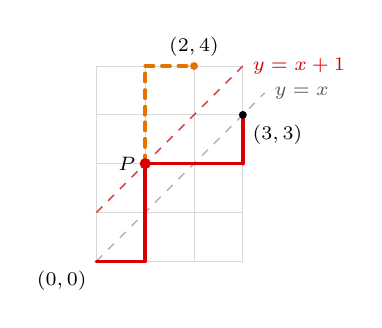
\begin{tikzpicture}
\draw[gray!30,line width=0.3pt] (0,0) -- (0,2.48);
\draw[gray!30,line width=0.3pt] (0.62,0) -- (0.62,2.48);
\draw[gray!30,line width=0.3pt] (1.24,0) -- (1.24,2.48);
\draw[gray!30,line width=0.3pt] (1.86,0) -- (1.86,2.48);
\draw[gray!30,line width=0.3pt] (0,0) -- (1.86,0);
\draw[gray!30,line width=0.3pt] (0,0.62) -- (1.86,0.62);
\draw[gray!30,line width=0.3pt] (0,1.24) -- (1.86,1.24);
\draw[gray!30,line width=0.3pt] (0,1.86) -- (1.86,1.86);
\draw[gray!30,line width=0.3pt] (0,2.48) -- (1.86,2.48);
\draw[gray!60,dashed,line width=0.5pt] (0,0) -- (2.139,2.139) node[right,font=\scriptsize,text=gray!70!black] {$y=x$};
\draw[cBad!80,dashed,line width=0.5pt] (0,0.62) -- (1.86,2.48) node[right,font=\scriptsize,text=cBad] {$y=x+1$};
\draw[cBad,line width=1.3pt,line cap=round] (0,0) -- (0.62,0);
\draw[cBad,line width=1.3pt,line cap=round] (0.62,0) -- (0.62,0.62);
\draw[cBad,line width=1.3pt,line cap=round] (0.62,0.62) -- (0.62,1.24);
\draw[cBad,line width=1.3pt,line cap=round] (0.62,1.24) -- (1.24,1.24);
\draw[cBad,line width=1.3pt,line cap=round] (1.24,1.24) -- (1.86,1.24);
\draw[cBad,line width=1.3pt,line cap=round] (1.86,1.24) -- (1.86,1.86);
\draw[cTop,line width=1.3pt,line cap=round,dashed] (0.62,1.24) -- (0.62,1.86);
\draw[cTop,line width=1.3pt,line cap=round,dashed] (0.62,1.86) -- (0.62,2.48);
\draw[cTop,line width=1.3pt,line cap=round,dashed] (0.62,2.48) -- (1.24,2.48);
\fill[cBad] (0.62,1.24) circle (0.07);
\node[left,font=\scriptsize] at (0.62,1.24) {$P$};
\fill (1.86,1.86) circle (0.05);
\node[below right,font=\scriptsize] at (1.86,1.86) {$(3,3)$};
\fill[cTop] (1.24,2.48) circle (0.05);
\node[above,font=\scriptsize] at (1.24,2.48) {$(2,4)$};
\node[below left,font=\scriptsize] at (0,0) {$(0,0)$};
\end{tikzpicture}}

\newcommand{\FigLatticeToDyck}{%
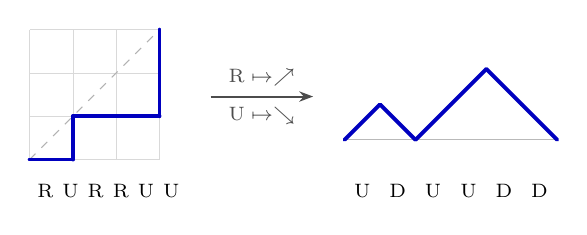
\begin{tikzpicture}
\draw[gray!30,line width=0.3pt] (0,0) -- (0,1.65);
\draw[gray!30,line width=0.3pt] (0.55,0) -- (0.55,1.65);
\draw[gray!30,line width=0.3pt] (1.1,0) -- (1.1,1.65);
\draw[gray!30,line width=0.3pt] (1.65,0) -- (1.65,1.65);
\draw[gray!30,line width=0.3pt] (0,0) -- (1.65,0);
\draw[gray!30,line width=0.3pt] (0,0.55) -- (1.65,0.55);
\draw[gray!30,line width=0.3pt] (0,1.1) -- (1.65,1.1);
\draw[gray!30,line width=0.3pt] (0,1.65) -- (1.65,1.65);
\draw[gray!60,dashed,line width=0.4pt] (0,0) -- (1.65,1.65);
\draw[cA,line width=1.4pt,line cap=round] (0,0) -- (0.55,0);
\draw[cA,line width=1.4pt,line cap=round] (0.55,0) -- (0.55,0.55);
\draw[cA,line width=1.4pt,line cap=round] (0.55,0.55) -- (1.1,0.55);
\draw[cA,line width=1.4pt,line cap=round] (1.1,0.55) -- (1.65,0.55);
\draw[cA,line width=1.4pt,line cap=round] (1.65,0.55) -- (1.65,1.1);
\draw[cA,line width=1.4pt,line cap=round] (1.65,1.1) -- (1.65,1.65);
\node[font=\scriptsize] at (0.2,-0.4) {R};
\node[font=\scriptsize] at (0.52,-0.4) {U};
\node[font=\scriptsize] at (0.84,-0.4) {R};
\node[font=\scriptsize] at (1.16,-0.4) {R};
\node[font=\scriptsize] at (1.48,-0.4) {U};
\node[font=\scriptsize] at (1.8,-0.4) {U};
\draw[-{Stealth[length=5pt]},line width=0.7pt,gray!60!black] (2.3,0.8) -- (3.6,0.8) node[midway,above,font=\scriptsize] {$\mathrm{R}\mapsto\nearrow$} node[midway,below,font=\scriptsize] {$\mathrm{U}\mapsto\searrow$};
\draw[gray!55,line width=0.4pt] (4,0.25) -- (6.7,0.25);
\draw[cA,line width=1.4pt,line cap=round] (4,0.25) -- (4.45,0.7);
\draw[cA,line width=1.4pt,line cap=round] (4.45,0.7) -- (4.9,0.25);
\draw[cA,line width=1.4pt,line cap=round] (4.9,0.25) -- (5.35,0.7);
\draw[cA,line width=1.4pt,line cap=round] (5.35,0.7) -- (5.8,1.15);
\draw[cA,line width=1.4pt,line cap=round] (5.8,1.15) -- (6.25,0.7);
\draw[cA,line width=1.4pt,line cap=round] (6.25,0.7) -- (6.7,0.25);
\node[font=\scriptsize] at (4.225,-0.4) {U};
\node[font=\scriptsize] at (4.675,-0.4) {D};
\node[font=\scriptsize] at (5.125,-0.4) {U};
\node[font=\scriptsize] at (5.575,-0.4) {U};
\node[font=\scriptsize] at (6.025,-0.4) {D};
\node[font=\scriptsize] at (6.475,-0.4) {D};
\end{tikzpicture}}

\newcommand{\FigDyckTable}{%
\begin{tikzpicture}
\node[anchor=west,font=\small] at (0,0.05) {$n=0$};
\draw[gray!55,line width=0.4pt] (1.35,0) -- (1.57,0);
\fill[cA] (1.35,0) circle (0.05);
\node[anchor=west,font=\scriptsize] at (1.7,0.02) {（空路徑）};
\node[anchor=west,font=\small] at (10.3,0.05) {1 種};
\node[anchor=west,font=\small] at (0,-0.92) {$n=1$};
\draw[gray!55,line width=0.4pt] (1.35,-0.97) -- (1.79,-0.97);
\draw[cTop,line width=1.2pt,line cap=round] (1.35,-0.97) -- (1.57,-0.75);
\draw[cTop,line width=1.2pt,line cap=round] (1.57,-0.75) -- (1.79,-0.97);
\node[anchor=west,font=\small] at (10.3,-0.92) {1 種};
\node[anchor=west,font=\small] at (0,-2.11) {$n=2$};
\draw[gray!55,line width=0.4pt] (1.35,-2.16) -- (2.23,-2.16);
\draw[cTop,line width=1.2pt,line cap=round] (1.35,-2.16) -- (1.57,-1.94);
\draw[cTop,line width=1.2pt,line cap=round] (1.57,-1.94) -- (1.79,-2.16);
\draw[cRight,line width=1.2pt,line cap=round] (1.79,-2.16) -- (2.01,-1.94);
\draw[cRight,line width=1.2pt,line cap=round] (2.01,-1.94) -- (2.23,-2.16);
\draw[gray!55,line width=0.4pt] (3.1,-2.16) -- (3.98,-2.16);
\draw[cTop,line width=1.2pt,line cap=round] (3.1,-2.16) -- (3.32,-1.94);
\draw[cLeft,line width=1.2pt,line cap=round] (3.32,-1.94) -- (3.54,-1.72);
\draw[cLeft,line width=1.2pt,line cap=round] (3.54,-1.72) -- (3.76,-1.94);
\draw[cTop,line width=1.2pt,line cap=round] (3.76,-1.94) -- (3.98,-2.16);
\node[anchor=west,font=\small] at (10.3,-2.11) {2 種};
\node[anchor=west,font=\small] at (0,-3.52) {$n=3$};
\draw[gray!55,line width=0.4pt] (1.35,-3.57) -- (2.67,-3.57);
\draw[cTop,line width=1.2pt,line cap=round] (1.35,-3.57) -- (1.57,-3.35);
\draw[cTop,line width=1.2pt,line cap=round] (1.57,-3.35) -- (1.79,-3.57);
\draw[cRight,line width=1.2pt,line cap=round] (1.79,-3.57) -- (2.01,-3.35);
\draw[cRight,line width=1.2pt,line cap=round] (2.01,-3.35) -- (2.23,-3.57);
\draw[cRight,line width=1.2pt,line cap=round] (2.23,-3.57) -- (2.45,-3.35);
\draw[cRight,line width=1.2pt,line cap=round] (2.45,-3.35) -- (2.67,-3.57);
\draw[gray!55,line width=0.4pt] (3.1,-3.57) -- (4.42,-3.57);
\draw[cTop,line width=1.2pt,line cap=round] (3.1,-3.57) -- (3.32,-3.35);
\draw[cTop,line width=1.2pt,line cap=round] (3.32,-3.35) -- (3.54,-3.57);
\draw[cRight,line width=1.2pt,line cap=round] (3.54,-3.57) -- (3.76,-3.35);
\draw[cRight,line width=1.2pt,line cap=round] (3.76,-3.35) -- (3.98,-3.13);
\draw[cRight,line width=1.2pt,line cap=round] (3.98,-3.13) -- (4.2,-3.35);
\draw[cRight,line width=1.2pt,line cap=round] (4.2,-3.35) -- (4.42,-3.57);
\draw[gray!55,line width=0.4pt] (4.85,-3.57) -- (6.17,-3.57);
\draw[cTop,line width=1.2pt,line cap=round] (4.85,-3.57) -- (5.07,-3.35);
\draw[cLeft,line width=1.2pt,line cap=round] (5.07,-3.35) -- (5.29,-3.13);
\draw[cLeft,line width=1.2pt,line cap=round] (5.29,-3.13) -- (5.51,-3.35);
\draw[cTop,line width=1.2pt,line cap=round] (5.51,-3.35) -- (5.73,-3.57);
\draw[cRight,line width=1.2pt,line cap=round] (5.73,-3.57) -- (5.95,-3.35);
\draw[cRight,line width=1.2pt,line cap=round] (5.95,-3.35) -- (6.17,-3.57);
\draw[gray!55,line width=0.4pt] (6.6,-3.57) -- (7.92,-3.57);
\draw[cTop,line width=1.2pt,line cap=round] (6.6,-3.57) -- (6.82,-3.35);
\draw[cLeft,line width=1.2pt,line cap=round] (6.82,-3.35) -- (7.04,-3.13);
\draw[cLeft,line width=1.2pt,line cap=round] (7.04,-3.13) -- (7.26,-3.35);
\draw[cLeft,line width=1.2pt,line cap=round] (7.26,-3.35) -- (7.48,-3.13);
\draw[cLeft,line width=1.2pt,line cap=round] (7.48,-3.13) -- (7.7,-3.35);
\draw[cTop,line width=1.2pt,line cap=round] (7.7,-3.35) -- (7.92,-3.57);
\draw[gray!55,line width=0.4pt] (8.35,-3.57) -- (9.67,-3.57);
\draw[cTop,line width=1.2pt,line cap=round] (8.35,-3.57) -- (8.57,-3.35);
\draw[cLeft,line width=1.2pt,line cap=round] (8.57,-3.35) -- (8.79,-3.13);
\draw[cLeft,line width=1.2pt,line cap=round] (8.79,-3.13) -- (9.01,-2.91);
\draw[cLeft,line width=1.2pt,line cap=round] (9.01,-2.91) -- (9.23,-3.13);
\draw[cLeft,line width=1.2pt,line cap=round] (9.23,-3.13) -- (9.45,-3.35);
\draw[cTop,line width=1.2pt,line cap=round] (9.45,-3.35) -- (9.67,-3.57);
\node[anchor=west,font=\small] at (10.3,-3.52) {5 種};
\end{tikzpicture}}

\newcommand{\FigDyckWords}{%
\begin{tikzpicture}
\node[anchor=west,font=\small] at (0,0.3) {Dyck 路徑};
\node[anchor=west,font=\small] at (0,-0.45) {括號字串};
\node[anchor=west,font=\small] at (0,-0.98) {開票順序};
\draw[gray!55,line width=0.4pt] (2.7,0) -- (4.14,0);
\draw[cTop,line width=1.2pt,line cap=round] (2.7,0) -- (2.94,0.24);
\draw[cTop,line width=1.2pt,line cap=round] (2.94,0.24) -- (3.18,0);
\draw[cRight,line width=1.2pt,line cap=round] (3.18,0) -- (3.42,0.24);
\draw[cRight,line width=1.2pt,line cap=round] (3.42,0.24) -- (3.66,0);
\draw[cRight,line width=1.2pt,line cap=round] (3.66,0) -- (3.9,0.24);
\draw[cRight,line width=1.2pt,line cap=round] (3.9,0.24) -- (4.14,0);
\node[font=\small] at (3.42,-0.45) {${\color{cTop}()}{\color{cRight}()()}$};
\node[font=\small] at (3.42,-0.98) {${\color{cTop}\mathrm{A}\mathrm{B}}{\color{cRight}\mathrm{A}\mathrm{B}\mathrm{A}\mathrm{B}}$};
\draw[gray!55,line width=0.4pt] (5.15,0) -- (6.59,0);
\draw[cTop,line width=1.2pt,line cap=round] (5.15,0) -- (5.39,0.24);
\draw[cTop,line width=1.2pt,line cap=round] (5.39,0.24) -- (5.63,0);
\draw[cRight,line width=1.2pt,line cap=round] (5.63,0) -- (5.87,0.24);
\draw[cRight,line width=1.2pt,line cap=round] (5.87,0.24) -- (6.11,0.48);
\draw[cRight,line width=1.2pt,line cap=round] (6.11,0.48) -- (6.35,0.24);
\draw[cRight,line width=1.2pt,line cap=round] (6.35,0.24) -- (6.59,0);
\node[font=\small] at (5.87,-0.45) {${\color{cTop}()}{\color{cRight}(())}$};
\node[font=\small] at (5.87,-0.98) {${\color{cTop}\mathrm{A}\mathrm{B}}{\color{cRight}\mathrm{A}\mathrm{A}\mathrm{B}\mathrm{B}}$};
\draw[gray!55,line width=0.4pt] (7.6,0) -- (9.04,0);
\draw[cTop,line width=1.2pt,line cap=round] (7.6,0) -- (7.84,0.24);
\draw[cLeft,line width=1.2pt,line cap=round] (7.84,0.24) -- (8.08,0.48);
\draw[cLeft,line width=1.2pt,line cap=round] (8.08,0.48) -- (8.32,0.24);
\draw[cTop,line width=1.2pt,line cap=round] (8.32,0.24) -- (8.56,0);
\draw[cRight,line width=1.2pt,line cap=round] (8.56,0) -- (8.8,0.24);
\draw[cRight,line width=1.2pt,line cap=round] (8.8,0.24) -- (9.04,0);
\node[font=\small] at (8.32,-0.45) {${\color{cTop}(}{\color{cLeft}()}{\color{cTop})}{\color{cRight}()}$};
\node[font=\small] at (8.32,-0.98) {${\color{cTop}\mathrm{A}}{\color{cLeft}\mathrm{A}\mathrm{B}}{\color{cTop}\mathrm{B}}{\color{cRight}\mathrm{A}\mathrm{B}}$};
\draw[gray!55,line width=0.4pt] (10.05,0) -- (11.49,0);
\draw[cTop,line width=1.2pt,line cap=round] (10.05,0) -- (10.29,0.24);
\draw[cLeft,line width=1.2pt,line cap=round] (10.29,0.24) -- (10.53,0.48);
\draw[cLeft,line width=1.2pt,line cap=round] (10.53,0.48) -- (10.77,0.24);
\draw[cLeft,line width=1.2pt,line cap=round] (10.77,0.24) -- (11.01,0.48);
\draw[cLeft,line width=1.2pt,line cap=round] (11.01,0.48) -- (11.25,0.24);
\draw[cTop,line width=1.2pt,line cap=round] (11.25,0.24) -- (11.49,0);
\node[font=\small] at (10.77,-0.45) {${\color{cTop}(}{\color{cLeft}()()}{\color{cTop})}$};
\node[font=\small] at (10.77,-0.98) {${\color{cTop}\mathrm{A}}{\color{cLeft}\mathrm{A}\mathrm{B}\mathrm{A}\mathrm{B}}{\color{cTop}\mathrm{B}}$};
\draw[gray!55,line width=0.4pt] (12.5,0) -- (13.94,0);
\draw[cTop,line width=1.2pt,line cap=round] (12.5,0) -- (12.74,0.24);
\draw[cLeft,line width=1.2pt,line cap=round] (12.74,0.24) -- (12.98,0.48);
\draw[cLeft,line width=1.2pt,line cap=round] (12.98,0.48) -- (13.22,0.72);
\draw[cLeft,line width=1.2pt,line cap=round] (13.22,0.72) -- (13.46,0.48);
\draw[cLeft,line width=1.2pt,line cap=round] (13.46,0.48) -- (13.7,0.24);
\draw[cTop,line width=1.2pt,line cap=round] (13.7,0.24) -- (13.94,0);
\node[font=\small] at (13.22,-0.45) {${\color{cTop}(}{\color{cLeft}(())}{\color{cTop})}$};
\node[font=\small] at (13.22,-0.98) {${\color{cTop}\mathrm{A}}{\color{cLeft}\mathrm{A}\mathrm{A}\mathrm{B}\mathrm{B}}{\color{cTop}\mathrm{B}}$};
\end{tikzpicture}}

\newcommand{\FigBallot}{%
\begin{tikzpicture}
\draw[gray!25,line width=0.3pt] (0,0.6) -- (4.8,0.6);
\draw[gray!25,line width=0.3pt] (0,1.2) -- (4.8,1.2);
\draw[-{Stealth[length=4pt]},gray!70!black,line width=0.5pt] (0,0) -- (5.2,0) node[right,font=\scriptsize] {已開的票數};
\draw[-{Stealth[length=4pt]},gray!70!black,line width=0.5pt] (0,0) -- (0,1.65) node[above,font=\scriptsize] {A 領先的票數};
\node[below,font=\scriptsize] at (0,0) {0};
\node[below,font=\scriptsize] at (0.8,0) {1};
\node[below,font=\scriptsize] at (1.6,0) {2};
\node[below,font=\scriptsize] at (2.4,0) {3};
\node[below,font=\scriptsize] at (3.2,0) {4};
\node[below,font=\scriptsize] at (4,0) {5};
\node[below,font=\scriptsize] at (4.8,0) {6};
\node[left,font=\scriptsize] at (0,0) {0};
\node[left,font=\scriptsize] at (0,0.6) {1};
\node[left,font=\scriptsize] at (0,1.2) {2};
\draw[cA,line width=1.4pt,line cap=round] (0,0) -- (0.8,0.6);
\node[above left,font=\scriptsize,inner sep=1.5pt] at (0.4,0.3) {A};
\draw[cA,line width=1.4pt,line cap=round] (0.8,0.6) -- (1.6,1.2);
\node[above left,font=\scriptsize,inner sep=1.5pt] at (1.2,0.9) {A};
\draw[cA,line width=1.4pt,line cap=round] (1.6,1.2) -- (2.4,0.6);
\node[above right,font=\scriptsize,inner sep=1.5pt] at (2,0.9) {B};
\draw[cA,line width=1.4pt,line cap=round] (2.4,0.6) -- (3.2,1.2);
\node[above left,font=\scriptsize,inner sep=1.5pt] at (2.8,0.9) {A};
\draw[cA,line width=1.4pt,line cap=round] (3.2,1.2) -- (4,0.6);
\node[above right,font=\scriptsize,inner sep=1.5pt] at (3.6,0.9) {B};
\draw[cA,line width=1.4pt,line cap=round] (4,0.6) -- (4.8,0);
\node[above right,font=\scriptsize,inner sep=1.5pt] at (4.4,0.3) {B};
\fill[cA] (0,0) circle (0.045);
\fill[cA] (0.8,0.6) circle (0.045);
\fill[cA] (1.6,1.2) circle (0.045);
\fill[cA] (2.4,0.6) circle (0.045);
\fill[cA] (3.2,1.2) circle (0.045);
\fill[cA] (4,0.6) circle (0.045);
\fill[cA] (4.8,0) circle (0.045);
\end{tikzpicture}}

\newcommand{\FigMatchRegions}{%
\begin{tikzpicture}
\fill[cLeft!22] (0,1) arc[start angle=90,end angle=30,radius=1.0] -- cycle;
\fill[cRight!20] (0.866,0.5) arc[start angle=30,end angle=-270,radius=1.0] -- cycle;
\draw[gray!65,line width=0.5pt] (0,0) circle (1.0);
\draw[cTop,line width=1.5pt,line cap=round] (0,1) -- (0.866,0.5);
\fill (0,1) circle (0.04);
\node[font=\scriptsize] at (0,1.22) {1};
\fill (0.866,0.5) circle (0.04);
\node[font=\scriptsize] at (1.057,0.61) {2};
\fill (0.866,-0.5) circle (0.04);
\node[font=\scriptsize] at (1.057,-0.61) {3};
\fill (0,-1) circle (0.04);
\node[font=\scriptsize] at (0,-1.22) {4};
\fill (-0.866,-0.5) circle (0.04);
\node[font=\scriptsize] at (-1.057,-0.61) {5};
\fill (-0.866,0.5) circle (0.04);
\node[font=\scriptsize] at (-1.057,0.61) {6};
\fill[cTop] (0,1) circle (0.07);
\node[font=\footnotesize,text=cLeft!85!black] at (0.74,1.282) {$C_0$};
\node[font=\footnotesize,text=cRight!85!black] at (-0.16,-0.277) {$C_2$};
\node[font=\footnotesize] at (0,-1.55) {點 1 配點 2：$\textcolor{cLeft}{C_0}\textcolor{cRight}{C_2}=2$};
\fill[cLeft!22] (3.75,1) arc[start angle=90,end angle=-90,radius=1.0] -- cycle;
\fill[cRight!20] (3.75,-1) arc[start angle=-90,end angle=-270,radius=1.0] -- cycle;
\draw[gray!65,line width=0.5pt] (3.75,0) circle (1.0);
\draw[cTop,line width=1.5pt,line cap=round] (3.75,1) -- (3.75,-1);
\fill (3.75,1) circle (0.04);
\node[font=\scriptsize] at (3.75,1.22) {1};
\fill (4.616,0.5) circle (0.04);
\node[font=\scriptsize] at (4.807,0.61) {2};
\fill (4.616,-0.5) circle (0.04);
\node[font=\scriptsize] at (4.807,-0.61) {3};
\fill (3.75,-1) circle (0.04);
\node[font=\scriptsize] at (3.75,-1.22) {4};
\fill (2.884,-0.5) circle (0.04);
\node[font=\scriptsize] at (2.693,-0.61) {5};
\fill (2.884,0.5) circle (0.04);
\node[font=\scriptsize] at (2.693,0.61) {6};
\fill[cTop] (3.75,1) circle (0.07);
\node[font=\footnotesize,text=cLeft!85!black] at (4.25,0) {$C_1$};
\node[font=\footnotesize,text=cRight!85!black] at (3.25,0) {$C_1$};
\node[font=\footnotesize] at (3.75,-1.55) {點 1 配點 4：$\textcolor{cLeft}{C_1}\textcolor{cRight}{C_1}=1$};
\fill[cLeft!22] (7.5,1) arc[start angle=90,end angle=-210,radius=1.0] -- cycle;
\fill[cRight!20] (6.634,0.5) arc[start angle=-210,end angle=-270,radius=1.0] -- cycle;
\draw[gray!65,line width=0.5pt] (7.5,0) circle (1.0);
\draw[cTop,line width=1.5pt,line cap=round] (7.5,1) -- (6.634,0.5);
\fill (7.5,1) circle (0.04);
\node[font=\scriptsize] at (7.5,1.22) {1};
\fill (8.366,0.5) circle (0.04);
\node[font=\scriptsize] at (8.557,0.61) {2};
\fill (8.366,-0.5) circle (0.04);
\node[font=\scriptsize] at (8.557,-0.61) {3};
\fill (7.5,-1) circle (0.04);
\node[font=\scriptsize] at (7.5,-1.22) {4};
\fill (6.634,-0.5) circle (0.04);
\node[font=\scriptsize] at (6.443,-0.61) {5};
\fill (6.634,0.5) circle (0.04);
\node[font=\scriptsize] at (6.443,0.61) {6};
\fill[cTop] (7.5,1) circle (0.07);
\node[font=\footnotesize,text=cLeft!85!black] at (7.66,-0.277) {$C_2$};
\node[font=\footnotesize,text=cRight!85!black] at (6.76,1.282) {$C_0$};
\node[font=\footnotesize] at (7.5,-1.55) {點 1 配點 6：$\textcolor{cLeft}{C_2}\textcolor{cRight}{C_0}=2$};
\end{tikzpicture}}

\newcommand{\FigOneNumber}{%
\begin{tikzpicture}
\node[font=\footnotesize] at (5,0.35) {$\textcolor{cLeft}{C_0}\textcolor{cRight}{C_2}$};
\node[font=\footnotesize] at (7.4,0.35) {$\textcolor{cLeft}{C_0}\textcolor{cRight}{C_2}$};
\node[font=\footnotesize] at (9.8,0.35) {$\textcolor{cLeft}{C_1}\textcolor{cRight}{C_1}$};
\node[font=\footnotesize] at (12.2,0.35) {$\textcolor{cLeft}{C_2}\textcolor{cRight}{C_0}$};
\node[font=\footnotesize] at (14.6,0.35) {$\textcolor{cLeft}{C_2}\textcolor{cRight}{C_0}$};
\draw[gray!35,line width=0.4pt] (0,0.08) -- (15.8,0.08);
\node[anchor=west,font=\small] at (0,-0.7) {凸五邊形的三角剖分};
\fill[cTop!38] (4.659,-1.225) -- (4.448,-0.576) -- (5.341,-1.225) -- cycle;
\fill[cRight!20] (4.448,-0.576) -- (5,-0.175) -- (5.552,-0.576) -- (5.341,-1.225) -- cycle;
\draw[gray!70,line width=0.6pt,line join=round] (4.659,-1.225) -- (4.448,-0.576) -- (5,-0.175) -- (5.552,-0.576) -- (5.341,-1.225) -- cycle;
\draw[cTop,line width=1.1pt,line cap=round] (4.448,-0.576) -- (5.341,-1.225);
\draw[cRight,line width=1.1pt,line cap=round] (5,-0.175) -- (5.341,-1.225);
\fill[black] (4.659,-1.225) circle (0.03);
\fill[black] (4.448,-0.576) circle (0.03);
\fill[black] (5,-0.175) circle (0.03);
\fill[black] (5.552,-0.576) circle (0.03);
\fill[black] (5.341,-1.225) circle (0.03);
\fill[cTop!38] (7.059,-1.225) -- (6.848,-0.576) -- (7.741,-1.225) -- cycle;
\fill[cRight!20] (6.848,-0.576) -- (7.4,-0.175) -- (7.952,-0.576) -- (7.741,-1.225) -- cycle;
\draw[gray!70,line width=0.6pt,line join=round] (7.059,-1.225) -- (6.848,-0.576) -- (7.4,-0.175) -- (7.952,-0.576) -- (7.741,-1.225) -- cycle;
\draw[cTop,line width=1.1pt,line cap=round] (6.848,-0.576) -- (7.741,-1.225);
\draw[cRight,line width=1.1pt,line cap=round] (6.848,-0.576) -- (7.952,-0.576);
\fill[black] (7.059,-1.225) circle (0.03);
\fill[black] (6.848,-0.576) circle (0.03);
\fill[black] (7.4,-0.175) circle (0.03);
\fill[black] (7.952,-0.576) circle (0.03);
\fill[black] (7.741,-1.225) circle (0.03);
\fill[cTop!38] (9.459,-1.225) -- (9.8,-0.175) -- (10.141,-1.225) -- cycle;
\fill[cLeft!22] (9.459,-1.225) -- (9.248,-0.576) -- (9.8,-0.175) -- cycle;
\fill[cRight!20] (9.8,-0.175) -- (10.352,-0.576) -- (10.141,-1.225) -- cycle;
\draw[gray!70,line width=0.6pt,line join=round] (9.459,-1.225) -- (9.248,-0.576) -- (9.8,-0.175) -- (10.352,-0.576) -- (10.141,-1.225) -- cycle;
\draw[cTop,line width=1.1pt,line cap=round] (9.459,-1.225) -- (9.8,-0.175);
\draw[cTop,line width=1.1pt,line cap=round] (9.8,-0.175) -- (10.141,-1.225);
\fill[black] (9.459,-1.225) circle (0.03);
\fill[black] (9.248,-0.576) circle (0.03);
\fill[black] (9.8,-0.175) circle (0.03);
\fill[black] (10.352,-0.576) circle (0.03);
\fill[black] (10.141,-1.225) circle (0.03);
\fill[cTop!38] (11.859,-1.225) -- (12.752,-0.576) -- (12.541,-1.225) -- cycle;
\fill[cLeft!22] (11.859,-1.225) -- (11.648,-0.576) -- (12.2,-0.175) -- (12.752,-0.576) -- cycle;
\draw[gray!70,line width=0.6pt,line join=round] (11.859,-1.225) -- (11.648,-0.576) -- (12.2,-0.175) -- (12.752,-0.576) -- (12.541,-1.225) -- cycle;
\draw[cTop,line width=1.1pt,line cap=round] (11.859,-1.225) -- (12.752,-0.576);
\draw[cLeft,line width=1.1pt,line cap=round] (11.648,-0.576) -- (12.752,-0.576);
\fill[black] (11.859,-1.225) circle (0.03);
\fill[black] (11.648,-0.576) circle (0.03);
\fill[black] (12.2,-0.175) circle (0.03);
\fill[black] (12.752,-0.576) circle (0.03);
\fill[black] (12.541,-1.225) circle (0.03);
\fill[cTop!38] (14.259,-1.225) -- (15.152,-0.576) -- (14.941,-1.225) -- cycle;
\fill[cLeft!22] (14.259,-1.225) -- (14.048,-0.576) -- (14.6,-0.175) -- (15.152,-0.576) -- cycle;
\draw[gray!70,line width=0.6pt,line join=round] (14.259,-1.225) -- (14.048,-0.576) -- (14.6,-0.175) -- (15.152,-0.576) -- (14.941,-1.225) -- cycle;
\draw[cTop,line width=1.1pt,line cap=round] (14.259,-1.225) -- (15.152,-0.576);
\draw[cLeft,line width=1.1pt,line cap=round] (14.259,-1.225) -- (14.6,-0.175);
\fill[black] (14.259,-1.225) circle (0.03);
\fill[black] (14.048,-0.576) circle (0.03);
\fill[black] (14.6,-0.175) circle (0.03);
\fill[black] (15.152,-0.576) circle (0.03);
\fill[black] (14.941,-1.225) circle (0.03);
\draw[gray!25,line width=0.3pt] (0,-1.4) -- (15.8,-1.4);
\node[anchor=west,font=\small] at (0,-1.71) {4 個因子的完全括號化};
\node[font=\small] at (5,-1.71) {${\color{cLeft}a}\mathbin{\color{cTop}\cdot}{\color{cRight}(b\cdot (c\cdot d))}$};
\node[font=\small] at (7.4,-1.71) {${\color{cLeft}a}\mathbin{\color{cTop}\cdot}{\color{cRight}((b\cdot c)\cdot d)}$};
\node[font=\small] at (9.8,-1.71) {${\color{cLeft}(a\cdot b)}\mathbin{\color{cTop}\cdot}{\color{cRight}(c\cdot d)}$};
\node[font=\small] at (12.2,-1.71) {${\color{cLeft}(a\cdot (b\cdot c))}\mathbin{\color{cTop}\cdot}{\color{cRight}d}$};
\node[font=\small] at (14.6,-1.71) {${\color{cLeft}((a\cdot b)\cdot c)}\mathbin{\color{cTop}\cdot}{\color{cRight}d}$};
\draw[gray!25,line width=0.3pt] (0,-2.02) -- (15.8,-2.02);
\node[anchor=west,font=\small] at (0,-2.72) {3 個內部節點的滿二元樹};
\draw[cTop,line width=0.8pt,line cap=round] (5,-2.185) -- (4.46,-2.545);
\draw[cTop,line width=0.8pt,line cap=round] (5,-2.185) -- (5.18,-2.545);
\draw[cRight,line width=0.8pt,line cap=round] (5.18,-2.545) -- (4.82,-2.905);
\draw[cRight,line width=0.8pt,line cap=round] (5.18,-2.545) -- (5.36,-2.905);
\draw[cRight,line width=0.8pt,line cap=round] (5.36,-2.905) -- (5.18,-3.265);
\draw[cRight,line width=0.8pt,line cap=round] (5.36,-2.905) -- (5.54,-3.265);
\fill[cTop] (5,-2.185) circle (0.05);
\fill[cRight] (5.18,-2.545) circle (0.05);
\fill[cRight] (5.36,-2.905) circle (0.05);
\fill[cLeft] (4.42,-2.585) rectangle (4.5,-2.505);
\fill[cRight] (4.78,-2.945) rectangle (4.86,-2.865);
\fill[cRight] (5.14,-3.305) rectangle (5.22,-3.225);
\fill[cRight] (5.5,-3.305) rectangle (5.58,-3.225);
\draw[cTop,line width=0.8pt,line cap=round] (7.4,-2.185) -- (6.86,-2.545);
\draw[cTop,line width=0.8pt,line cap=round] (7.4,-2.185) -- (7.58,-2.545);
\draw[cRight,line width=0.8pt,line cap=round] (7.4,-2.905) -- (7.22,-3.265);
\draw[cRight,line width=0.8pt,line cap=round] (7.4,-2.905) -- (7.58,-3.265);
\draw[cRight,line width=0.8pt,line cap=round] (7.58,-2.545) -- (7.4,-2.905);
\draw[cRight,line width=0.8pt,line cap=round] (7.58,-2.545) -- (7.94,-2.905);
\fill[cTop] (7.4,-2.185) circle (0.05);
\fill[cRight] (7.4,-2.905) circle (0.05);
\fill[cRight] (7.58,-2.545) circle (0.05);
\fill[cLeft] (6.82,-2.585) rectangle (6.9,-2.505);
\fill[cRight] (7.18,-3.305) rectangle (7.26,-3.225);
\fill[cRight] (7.54,-3.305) rectangle (7.62,-3.225);
\fill[cRight] (7.9,-2.945) rectangle (7.98,-2.865);
\draw[cLeft,line width=0.8pt,line cap=round] (9.44,-2.725) -- (9.26,-3.085);
\draw[cLeft,line width=0.8pt,line cap=round] (9.44,-2.725) -- (9.62,-3.085);
\draw[cTop,line width=0.8pt,line cap=round] (9.8,-2.365) -- (9.44,-2.725);
\draw[cTop,line width=0.8pt,line cap=round] (9.8,-2.365) -- (10.16,-2.725);
\draw[cRight,line width=0.8pt,line cap=round] (10.16,-2.725) -- (9.98,-3.085);
\draw[cRight,line width=0.8pt,line cap=round] (10.16,-2.725) -- (10.34,-3.085);
\fill[cLeft] (9.44,-2.725) circle (0.05);
\fill[cTop] (9.8,-2.365) circle (0.05);
\fill[cRight] (10.16,-2.725) circle (0.05);
\fill[cLeft] (9.22,-3.125) rectangle (9.3,-3.045);
\fill[cLeft] (9.58,-3.125) rectangle (9.66,-3.045);
\fill[cRight] (9.94,-3.125) rectangle (10.02,-3.045);
\fill[cRight] (10.3,-3.125) rectangle (10.38,-3.045);
\draw[cLeft,line width=0.8pt,line cap=round] (12.02,-2.545) -- (11.66,-2.905);
\draw[cLeft,line width=0.8pt,line cap=round] (12.02,-2.545) -- (12.2,-2.905);
\draw[cLeft,line width=0.8pt,line cap=round] (12.2,-2.905) -- (12.02,-3.265);
\draw[cLeft,line width=0.8pt,line cap=round] (12.2,-2.905) -- (12.38,-3.265);
\draw[cTop,line width=0.8pt,line cap=round] (12.2,-2.185) -- (12.02,-2.545);
\draw[cTop,line width=0.8pt,line cap=round] (12.2,-2.185) -- (12.74,-2.545);
\fill[cLeft] (12.02,-2.545) circle (0.05);
\fill[cLeft] (12.2,-2.905) circle (0.05);
\fill[cTop] (12.2,-2.185) circle (0.05);
\fill[cLeft] (11.62,-2.945) rectangle (11.7,-2.865);
\fill[cLeft] (11.98,-3.305) rectangle (12.06,-3.225);
\fill[cLeft] (12.34,-3.305) rectangle (12.42,-3.225);
\fill[cRight] (12.7,-2.585) rectangle (12.78,-2.505);
\draw[cLeft,line width=0.8pt,line cap=round] (14.24,-2.905) -- (14.06,-3.265);
\draw[cLeft,line width=0.8pt,line cap=round] (14.24,-2.905) -- (14.42,-3.265);
\draw[cLeft,line width=0.8pt,line cap=round] (14.42,-2.545) -- (14.24,-2.905);
\draw[cLeft,line width=0.8pt,line cap=round] (14.42,-2.545) -- (14.78,-2.905);
\draw[cTop,line width=0.8pt,line cap=round] (14.6,-2.185) -- (14.42,-2.545);
\draw[cTop,line width=0.8pt,line cap=round] (14.6,-2.185) -- (15.14,-2.545);
\fill[cLeft] (14.24,-2.905) circle (0.05);
\fill[cLeft] (14.42,-2.545) circle (0.05);
\fill[cTop] (14.6,-2.185) circle (0.05);
\fill[cLeft] (14.02,-3.305) rectangle (14.1,-3.225);
\fill[cLeft] (14.38,-3.305) rectangle (14.46,-3.225);
\fill[cLeft] (14.74,-2.945) rectangle (14.82,-2.865);
\fill[cRight] (15.1,-2.585) rectangle (15.18,-2.505);
\draw[gray!25,line width=0.3pt] (0,-3.42) -- (15.8,-3.42);
\node[anchor=west,font=\small] at (0,-3.995) {不越過 $y=x$ 的格子路徑};
\draw[gray!30,line width=0.3pt] (4.55,-4.445) -- (4.55,-3.545);
\draw[gray!30,line width=0.3pt] (4.85,-4.445) -- (4.85,-3.545);
\draw[gray!30,line width=0.3pt] (5.15,-4.445) -- (5.15,-3.545);
\draw[gray!30,line width=0.3pt] (5.45,-4.445) -- (5.45,-3.545);
\draw[gray!30,line width=0.3pt] (4.55,-4.445) -- (5.45,-4.445);
\draw[gray!30,line width=0.3pt] (4.55,-4.145) -- (5.45,-4.145);
\draw[gray!30,line width=0.3pt] (4.55,-3.845) -- (5.45,-3.845);
\draw[gray!30,line width=0.3pt] (4.55,-3.545) -- (5.45,-3.545);
\draw[gray!60,dashed,line width=0.4pt] (4.55,-4.445) -- (5.45,-3.545);
\draw[cTop,line width=1.2pt,line cap=round] (4.55,-4.445) -- (4.85,-4.445);
\draw[cTop,line width=1.2pt,line cap=round] (4.85,-4.445) -- (4.85,-4.145);
\draw[cRight,line width=1.2pt,line cap=round] (4.85,-4.145) -- (5.15,-4.145);
\draw[cRight,line width=1.2pt,line cap=round] (5.15,-4.145) -- (5.15,-3.845);
\draw[cRight,line width=1.2pt,line cap=round] (5.15,-3.845) -- (5.45,-3.845);
\draw[cRight,line width=1.2pt,line cap=round] (5.45,-3.845) -- (5.45,-3.545);
\draw[gray!30,line width=0.3pt] (6.95,-4.445) -- (6.95,-3.545);
\draw[gray!30,line width=0.3pt] (7.25,-4.445) -- (7.25,-3.545);
\draw[gray!30,line width=0.3pt] (7.55,-4.445) -- (7.55,-3.545);
\draw[gray!30,line width=0.3pt] (7.85,-4.445) -- (7.85,-3.545);
\draw[gray!30,line width=0.3pt] (6.95,-4.445) -- (7.85,-4.445);
\draw[gray!30,line width=0.3pt] (6.95,-4.145) -- (7.85,-4.145);
\draw[gray!30,line width=0.3pt] (6.95,-3.845) -- (7.85,-3.845);
\draw[gray!30,line width=0.3pt] (6.95,-3.545) -- (7.85,-3.545);
\draw[gray!60,dashed,line width=0.4pt] (6.95,-4.445) -- (7.85,-3.545);
\draw[cTop,line width=1.2pt,line cap=round] (6.95,-4.445) -- (7.25,-4.445);
\draw[cTop,line width=1.2pt,line cap=round] (7.25,-4.445) -- (7.25,-4.145);
\draw[cRight,line width=1.2pt,line cap=round] (7.25,-4.145) -- (7.55,-4.145);
\draw[cRight,line width=1.2pt,line cap=round] (7.55,-4.145) -- (7.85,-4.145);
\draw[cRight,line width=1.2pt,line cap=round] (7.85,-4.145) -- (7.85,-3.845);
\draw[cRight,line width=1.2pt,line cap=round] (7.85,-3.845) -- (7.85,-3.545);
\draw[gray!30,line width=0.3pt] (9.35,-4.445) -- (9.35,-3.545);
\draw[gray!30,line width=0.3pt] (9.65,-4.445) -- (9.65,-3.545);
\draw[gray!30,line width=0.3pt] (9.95,-4.445) -- (9.95,-3.545);
\draw[gray!30,line width=0.3pt] (10.25,-4.445) -- (10.25,-3.545);
\draw[gray!30,line width=0.3pt] (9.35,-4.445) -- (10.25,-4.445);
\draw[gray!30,line width=0.3pt] (9.35,-4.145) -- (10.25,-4.145);
\draw[gray!30,line width=0.3pt] (9.35,-3.845) -- (10.25,-3.845);
\draw[gray!30,line width=0.3pt] (9.35,-3.545) -- (10.25,-3.545);
\draw[gray!60,dashed,line width=0.4pt] (9.35,-4.445) -- (10.25,-3.545);
\draw[cTop,line width=1.2pt,line cap=round] (9.35,-4.445) -- (9.65,-4.445);
\draw[cLeft,line width=1.2pt,line cap=round] (9.65,-4.445) -- (9.95,-4.445);
\draw[cLeft,line width=1.2pt,line cap=round] (9.95,-4.445) -- (9.95,-4.145);
\draw[cTop,line width=1.2pt,line cap=round] (9.95,-4.145) -- (9.95,-3.845);
\draw[cRight,line width=1.2pt,line cap=round] (9.95,-3.845) -- (10.25,-3.845);
\draw[cRight,line width=1.2pt,line cap=round] (10.25,-3.845) -- (10.25,-3.545);
\draw[gray!30,line width=0.3pt] (11.75,-4.445) -- (11.75,-3.545);
\draw[gray!30,line width=0.3pt] (12.05,-4.445) -- (12.05,-3.545);
\draw[gray!30,line width=0.3pt] (12.35,-4.445) -- (12.35,-3.545);
\draw[gray!30,line width=0.3pt] (12.65,-4.445) -- (12.65,-3.545);
\draw[gray!30,line width=0.3pt] (11.75,-4.445) -- (12.65,-4.445);
\draw[gray!30,line width=0.3pt] (11.75,-4.145) -- (12.65,-4.145);
\draw[gray!30,line width=0.3pt] (11.75,-3.845) -- (12.65,-3.845);
\draw[gray!30,line width=0.3pt] (11.75,-3.545) -- (12.65,-3.545);
\draw[gray!60,dashed,line width=0.4pt] (11.75,-4.445) -- (12.65,-3.545);
\draw[cTop,line width=1.2pt,line cap=round] (11.75,-4.445) -- (12.05,-4.445);
\draw[cLeft,line width=1.2pt,line cap=round] (12.05,-4.445) -- (12.35,-4.445);
\draw[cLeft,line width=1.2pt,line cap=round] (12.35,-4.445) -- (12.35,-4.145);
\draw[cLeft,line width=1.2pt,line cap=round] (12.35,-4.145) -- (12.65,-4.145);
\draw[cLeft,line width=1.2pt,line cap=round] (12.65,-4.145) -- (12.65,-3.845);
\draw[cTop,line width=1.2pt,line cap=round] (12.65,-3.845) -- (12.65,-3.545);
\draw[gray!30,line width=0.3pt] (14.15,-4.445) -- (14.15,-3.545);
\draw[gray!30,line width=0.3pt] (14.45,-4.445) -- (14.45,-3.545);
\draw[gray!30,line width=0.3pt] (14.75,-4.445) -- (14.75,-3.545);
\draw[gray!30,line width=0.3pt] (15.05,-4.445) -- (15.05,-3.545);
\draw[gray!30,line width=0.3pt] (14.15,-4.445) -- (15.05,-4.445);
\draw[gray!30,line width=0.3pt] (14.15,-4.145) -- (15.05,-4.145);
\draw[gray!30,line width=0.3pt] (14.15,-3.845) -- (15.05,-3.845);
\draw[gray!30,line width=0.3pt] (14.15,-3.545) -- (15.05,-3.545);
\draw[gray!60,dashed,line width=0.4pt] (14.15,-4.445) -- (15.05,-3.545);
\draw[cTop,line width=1.2pt,line cap=round] (14.15,-4.445) -- (14.45,-4.445);
\draw[cLeft,line width=1.2pt,line cap=round] (14.45,-4.445) -- (14.75,-4.445);
\draw[cLeft,line width=1.2pt,line cap=round] (14.75,-4.445) -- (15.05,-4.445);
\draw[cLeft,line width=1.2pt,line cap=round] (15.05,-4.445) -- (15.05,-4.145);
\draw[cLeft,line width=1.2pt,line cap=round] (15.05,-4.145) -- (15.05,-3.845);
\draw[cTop,line width=1.2pt,line cap=round] (15.05,-3.845) -- (15.05,-3.545);
\draw[gray!25,line width=0.3pt] (0,-4.57) -- (15.8,-4.57);
\node[anchor=west,font=\small] at (0,-4.995) {半長 3 的 Dyck 路徑};
\draw[gray!55,line width=0.4pt] (4.4,-5.095) -- (5.6,-5.095);
\draw[cTop,line width=1.2pt,line cap=round] (4.4,-5.095) -- (4.6,-4.895);
\draw[cTop,line width=1.2pt,line cap=round] (4.6,-4.895) -- (4.8,-5.095);
\draw[cRight,line width=1.2pt,line cap=round] (4.8,-5.095) -- (5,-4.895);
\draw[cRight,line width=1.2pt,line cap=round] (5,-4.895) -- (5.2,-5.095);
\draw[cRight,line width=1.2pt,line cap=round] (5.2,-5.095) -- (5.4,-4.895);
\draw[cRight,line width=1.2pt,line cap=round] (5.4,-4.895) -- (5.6,-5.095);
\draw[gray!55,line width=0.4pt] (6.8,-5.195) -- (8,-5.195);
\draw[cTop,line width=1.2pt,line cap=round] (6.8,-5.195) -- (7,-4.995);
\draw[cTop,line width=1.2pt,line cap=round] (7,-4.995) -- (7.2,-5.195);
\draw[cRight,line width=1.2pt,line cap=round] (7.2,-5.195) -- (7.4,-4.995);
\draw[cRight,line width=1.2pt,line cap=round] (7.4,-4.995) -- (7.6,-4.795);
\draw[cRight,line width=1.2pt,line cap=round] (7.6,-4.795) -- (7.8,-4.995);
\draw[cRight,line width=1.2pt,line cap=round] (7.8,-4.995) -- (8,-5.195);
\draw[gray!55,line width=0.4pt] (9.2,-5.195) -- (10.4,-5.195);
\draw[cTop,line width=1.2pt,line cap=round] (9.2,-5.195) -- (9.4,-4.995);
\draw[cLeft,line width=1.2pt,line cap=round] (9.4,-4.995) -- (9.6,-4.795);
\draw[cLeft,line width=1.2pt,line cap=round] (9.6,-4.795) -- (9.8,-4.995);
\draw[cTop,line width=1.2pt,line cap=round] (9.8,-4.995) -- (10,-5.195);
\draw[cRight,line width=1.2pt,line cap=round] (10,-5.195) -- (10.2,-4.995);
\draw[cRight,line width=1.2pt,line cap=round] (10.2,-4.995) -- (10.4,-5.195);
\draw[gray!55,line width=0.4pt] (11.6,-5.195) -- (12.8,-5.195);
\draw[cTop,line width=1.2pt,line cap=round] (11.6,-5.195) -- (11.8,-4.995);
\draw[cLeft,line width=1.2pt,line cap=round] (11.8,-4.995) -- (12,-4.795);
\draw[cLeft,line width=1.2pt,line cap=round] (12,-4.795) -- (12.2,-4.995);
\draw[cLeft,line width=1.2pt,line cap=round] (12.2,-4.995) -- (12.4,-4.795);
\draw[cLeft,line width=1.2pt,line cap=round] (12.4,-4.795) -- (12.6,-4.995);
\draw[cTop,line width=1.2pt,line cap=round] (12.6,-4.995) -- (12.8,-5.195);
\draw[gray!55,line width=0.4pt] (14,-5.295) -- (15.2,-5.295);
\draw[cTop,line width=1.2pt,line cap=round] (14,-5.295) -- (14.2,-5.095);
\draw[cLeft,line width=1.2pt,line cap=round] (14.2,-5.095) -- (14.4,-4.895);
\draw[cLeft,line width=1.2pt,line cap=round] (14.4,-4.895) -- (14.6,-4.695);
\draw[cLeft,line width=1.2pt,line cap=round] (14.6,-4.695) -- (14.8,-4.895);
\draw[cLeft,line width=1.2pt,line cap=round] (14.8,-4.895) -- (15,-5.095);
\draw[cTop,line width=1.2pt,line cap=round] (15,-5.095) -- (15.2,-5.295);
\draw[gray!25,line width=0.3pt] (0,-5.42) -- (15.8,-5.42);
\node[anchor=west,font=\small] at (0,-5.71) {3 對括號的平衡字串};
\node[font=\small] at (5,-5.71) {${\color{cTop}()}{\color{cRight}()()}$};
\node[font=\small] at (7.4,-5.71) {${\color{cTop}()}{\color{cRight}(())}$};
\node[font=\small] at (9.8,-5.71) {${\color{cTop}(}{\color{cLeft}()}{\color{cTop})}{\color{cRight}()}$};
\node[font=\small] at (12.2,-5.71) {${\color{cTop}(}{\color{cLeft}()()}{\color{cTop})}$};
\node[font=\small] at (14.6,-5.71) {${\color{cTop}(}{\color{cLeft}(())}{\color{cTop})}$};
\draw[gray!25,line width=0.3pt] (0,-6) -- (15.8,-6);
\node[anchor=west,font=\small] at (0,-6.29) {兩人各 3 票的開票順序};
\node[font=\small] at (5,-6.29) {${\color{cTop}\mathrm{A}\mathrm{B}}{\color{cRight}\mathrm{A}\mathrm{B}\mathrm{A}\mathrm{B}}$};
\node[font=\small] at (7.4,-6.29) {${\color{cTop}\mathrm{A}\mathrm{B}}{\color{cRight}\mathrm{A}\mathrm{A}\mathrm{B}\mathrm{B}}$};
\node[font=\small] at (9.8,-6.29) {${\color{cTop}\mathrm{A}}{\color{cLeft}\mathrm{A}\mathrm{B}}{\color{cTop}\mathrm{B}}{\color{cRight}\mathrm{A}\mathrm{B}}$};
\node[font=\small] at (12.2,-6.29) {${\color{cTop}\mathrm{A}}{\color{cLeft}\mathrm{A}\mathrm{B}\mathrm{A}\mathrm{B}}{\color{cTop}\mathrm{B}}$};
\node[font=\small] at (14.6,-6.29) {${\color{cTop}\mathrm{A}}{\color{cLeft}\mathrm{A}\mathrm{A}\mathrm{B}\mathrm{B}}{\color{cTop}\mathrm{B}}$};
\draw[gray!25,line width=0.3pt] (0,-6.58) -- (15.8,-6.58);
\node[anchor=west,font=\small] at (0,-7.255) {圓周 6 點的不交叉配對};
\draw[gray!65,line width=0.5pt] (5,-7.27) circle (0.52);
\draw[cTop,line width=1.1pt,line cap=round] (5,-6.75) -- (5.45,-7.01);
\draw[cRight,line width=1.1pt,line cap=round] (5.45,-7.53) -- (5,-7.79);
\draw[cRight,line width=1.1pt,line cap=round] (4.55,-7.53) -- (4.55,-7.01);
\fill[black] (5,-6.75) circle (0.035);
\fill[black] (5.45,-7.01) circle (0.035);
\fill[black] (5.45,-7.53) circle (0.035);
\fill[black] (5,-7.79) circle (0.035);
\fill[black] (4.55,-7.53) circle (0.035);
\fill[black] (4.55,-7.01) circle (0.035);
\fill[cTop] (5,-6.75) circle (0.065);
\draw[gray!65,line width=0.5pt] (7.4,-7.27) circle (0.52);
\draw[cTop,line width=1.1pt,line cap=round] (7.4,-6.75) -- (7.85,-7.01);
\draw[cRight,line width=1.1pt,line cap=round] (7.85,-7.53) -- (6.95,-7.01);
\draw[cRight,line width=1.1pt,line cap=round] (7.4,-7.79) -- (6.95,-7.53);
\fill[black] (7.4,-6.75) circle (0.035);
\fill[black] (7.85,-7.01) circle (0.035);
\fill[black] (7.85,-7.53) circle (0.035);
\fill[black] (7.4,-7.79) circle (0.035);
\fill[black] (6.95,-7.53) circle (0.035);
\fill[black] (6.95,-7.01) circle (0.035);
\fill[cTop] (7.4,-6.75) circle (0.065);
\draw[gray!65,line width=0.5pt] (9.8,-7.27) circle (0.52);
\draw[cTop,line width=1.1pt,line cap=round] (9.8,-6.75) -- (9.8,-7.79);
\draw[cLeft,line width=1.1pt,line cap=round] (10.25,-7.01) -- (10.25,-7.53);
\draw[cRight,line width=1.1pt,line cap=round] (9.35,-7.53) -- (9.35,-7.01);
\fill[black] (9.8,-6.75) circle (0.035);
\fill[black] (10.25,-7.01) circle (0.035);
\fill[black] (10.25,-7.53) circle (0.035);
\fill[black] (9.8,-7.79) circle (0.035);
\fill[black] (9.35,-7.53) circle (0.035);
\fill[black] (9.35,-7.01) circle (0.035);
\fill[cTop] (9.8,-6.75) circle (0.065);
\draw[gray!65,line width=0.5pt] (12.2,-7.27) circle (0.52);
\draw[cTop,line width=1.1pt,line cap=round] (12.2,-6.75) -- (11.75,-7.01);
\draw[cLeft,line width=1.1pt,line cap=round] (12.65,-7.01) -- (12.65,-7.53);
\draw[cLeft,line width=1.1pt,line cap=round] (12.2,-7.79) -- (11.75,-7.53);
\fill[black] (12.2,-6.75) circle (0.035);
\fill[black] (12.65,-7.01) circle (0.035);
\fill[black] (12.65,-7.53) circle (0.035);
\fill[black] (12.2,-7.79) circle (0.035);
\fill[black] (11.75,-7.53) circle (0.035);
\fill[black] (11.75,-7.01) circle (0.035);
\fill[cTop] (12.2,-6.75) circle (0.065);
\draw[gray!65,line width=0.5pt] (14.6,-7.27) circle (0.52);
\draw[cTop,line width=1.1pt,line cap=round] (14.6,-6.75) -- (14.15,-7.01);
\draw[cLeft,line width=1.1pt,line cap=round] (15.05,-7.01) -- (14.15,-7.53);
\draw[cLeft,line width=1.1pt,line cap=round] (15.05,-7.53) -- (14.6,-7.79);
\fill[black] (14.6,-6.75) circle (0.035);
\fill[black] (15.05,-7.01) circle (0.035);
\fill[black] (15.05,-7.53) circle (0.035);
\fill[black] (14.6,-7.79) circle (0.035);
\fill[black] (14.15,-7.53) circle (0.035);
\fill[black] (14.15,-7.01) circle (0.035);
\fill[cTop] (14.6,-6.75) circle (0.065);
\draw[gray!25,line width=0.3pt] (0,-7.93) -- (15.8,-7.93);
\end{tikzpicture}}


\title{\textbf{廣義卡塔蘭數的新組合詮釋}\\[0.3em]\large W.~Chu (1987) 論文導讀}
\author{\normalsize 原文：Wenchang Chu, \emph{A new combinatorial interpretation for generalized Catalan number},\\\normalsize
\emph{Discrete Mathematics} \textbf{65} (1987) 91--94.\\[0.2em]\normalsize
第 1 節另參考：A.~Selimi, M.~Saračević, \emph{Catalan Numbers and Applications},\\\normalsize
\emph{Vision International Scientific Journal} \textbf{4}(1) (2019) 99--114.}
\date{}

\begin{document}
\maketitle
\vspace{-2.5em}

\begin{keybox}[一頁看懂]
\textbf{問題。}在圓周上放一些點，把它們分成若干「群組」，並規定各種大小的群組各要幾個。
把同一群組的點連成一個凸多邊形（2 個點就是一條弦）。
要求\textbf{不同群組的多邊形在圓內不可以相交}。請問有幾種分法？

\textbf{答案。}恰好是「廣義卡塔蘭數」$\Cv(\vn)$，有一條乾淨的公式：
\[
\Cv(\vn)=\frac{N!}{n_1!\,n_2!\cdots n_k!\;(N+1-b)!},\qquad
N=\text{總點數},\quad b=\text{群組總數}.
\]

\textbf{證明的三步。}
\begin{enumerate}[leftmargin=1.6em]
  \item \textbf{固定一個點}，看它所在的群組。這個群組（$v_i$ 個點）把其餘的點切成 $v_i$ 段，各段互不干擾。
  \item 「互不干擾」翻譯成代數就是\textbf{相乘}，於是得到生成函數的方程
        $D=1+x_1D^{v_1}+\cdots+x_kD^{v_k}$。
  \item 用 Raney 公式檢查：由廣義卡塔蘭數組成的生成函數 $C$ 也滿足同一條方程。
        這條方程的解只有一個，所以 $D=C$，證畢。
\end{enumerate}
\end{keybox}

\setcounter{tocdepth}{1}
\begingroup
\setlength{\parskip}{0pt}  % 目錄排緊一點，才能和「一頁看懂」放在同一頁
\tableofcontents
\endgroup
\newpage

% =====================================================================
\section{熱身：經典卡塔蘭數——同一個數，許多種物件}\label{sec:catalan}
% =====================================================================

這一節先把經典卡塔蘭數講清楚：它數的是哪些東西，以及為什麼這些東西的數目都一樣。
重點不在多背幾個例子，而是看出它們共同的結構——
\textbf{固定一個「根」，剩下的部分切成左、右兩個獨立的小問題}。
Chu 的論文就是把「切成兩塊」推廣成「切成 $v_i$ 塊」。

本節對應 manim 演示的卡塔蘭基礎模組（場景 00a--00m），第 1.$k$ 小節對應其中第 $k$ 個場景。
內容主要參考 Selimi 與 Saračević 的介紹文（書目在標題下方），以〔來源 第 $p$ 頁〕標示它的頁碼；
〔原文 第 $p$ 頁〕仍然指 Chu 的論文。

\begin{center}
\small
\begin{tabular}{@{}lll@{\qquad\qquad}lll@{}}
\toprule
小節 & 內容 & 動畫 & 小節 & 內容 & 動畫\\
\midrule
1.1 & 數列與公式 & 00a & 1.8 & 平衡括號 & 00h\\
1.2 & 凸多邊形的三角剖分 & 00b & 1.9 & 投票問題 & 00i\\
1.3 & 固定底邊：卡塔蘭遞迴 & 00c & 1.10 & 圓上的不交叉配對 & 00j\\
1.4 & 完全括號化 & 00d & 1.11 & 同一個 $C_n$：一一對應 & 00k\\
1.5 & 滿二元樹 & 00e & 1.12 & 生成函數 $C=1+xC^2$ & 00l\\
1.6 & 格子路徑與反射原理 & 00f & 1.13 & 接到 Chu 的推廣 & 00m\\
1.7 & Dyck 路徑 & 00g & & & \\
\bottomrule
\end{tabular}
\end{center}

% ---------------------------------------------------------------------
\subsection{數列與公式}

卡塔蘭數（Catalan number）的定義是 \src{第 100 頁，式 (1.1)}
\[
C_n=\frac{(2n)!}{(n+1)!\,n!}=\frac{1}{n+1}\binom{2n}{n},\qquad n\ge 0 .
\]
\begin{center}
\begin{tabular}{c|ccccccccccc}
$n$ & 0 & 1 & 2 & 3 & 4 & 5 & 6 & 7 & 8 & 9 & 10\\
\hline
$C_n$ & 1 & 1 & 2 & 5 & 14 & 42 & 132 & 429 & 1430 & 4862 & 16796
\end{tabular}
\end{center}
另一個常用的寫法是兩個二項式係數相減 \src{第 101 頁，式 (1.2)}：
\[
C_n=\binom{2n}{n}-\binom{2n}{n-1}\qquad(n\ge1).
\]
為什麼要減掉 $\binom{2n}{n-1}$，第 1.6 節用格子路徑解釋。

它在組合數學裡到處出現。原文第一段就提到它有大約五十種不同的詮釋：
括號的加法（非結合代數）、凸多邊形的切割、投票問題、格子路徑、隨機漫步、平面樹等等 \paper{第 91 頁}。

\textbf{一點歷史} \src{第 100--101 頁}。
\begin{itemize}
  \item Euler 與 Segner（18 世紀）研究凸多邊形的三角剖分；Segner 給出遞迴式（第 1.3 節）。
  \item 明安圖（1692--1763，清代的蒙古族數學家）約在 1730 年獨立用到這串數。
        他把 $\sin 2x$、$\sin 4x$ 展開成 $\sin x$ 的冪級數，例如
        \[
        \sin 2x=2\sin x-\sum_{k\ge1}\frac{C_{k-1}}{4^{k-1}}\,\sin^{2k+1}x
        =2\sin x-\sin^3x-\tfrac14\sin^5x-\tfrac18\sin^7x-\cdots .
        \]
        他的著作以中文寫成，西方很久之後才知道。
  \item Catalan（1814--1894）在 1838 年研究括號問題；這串數後來以他命名。
\end{itemize}

% ---------------------------------------------------------------------
\subsection{凸多邊形的三角剖分}

用互不相交的對角線把凸多邊形切成三角形，稱為一種\textbf{三角剖分}。
凸 $m$ 邊形的三角剖分數記為 $T_m$ \src{第 101--102 頁}：
三角形本身已經切好，$T_3=1$；四邊形有兩條對角線，任選一條，$T_4=2$；
五邊形有 5 種，六邊形有 14 種（圖~\ref{fig:hexgroups}）。

\begin{figure}[H]
\centering
\FigTriSmall
\caption{三角形、凸四邊形、凸五邊形的所有三角剖分。}
\label{fig:trismall}
\end{figure}

凸 $m$ 邊形的每一種三角剖分都恰好用 $m-3$ 條對角線，切出 $m-2$ 個三角形。
數字 $1,2,5,14$ 正是卡塔蘭數：

\begin{thmbox}[三角剖分]
凸 $(n+2)$ 邊形的三角剖分恰有 $C_n$ 種，也就是 $T_{n+2}=C_n$。
\end{thmbox}

注意指標：凸 $m$ 邊形對應的是 $C_{m-2}$（$n$ 是三角形的個數）。證明在下一小節。

% ---------------------------------------------------------------------
\subsection{固定底邊：卡塔蘭遞迴}

把凸 $(n+2)$ 邊形的頂點依序編號為 $0,1,\ldots,n+1$，選定邊 $\{0,n+1\}$ 當作\textbf{底邊}
\src{第 102--103 頁}。
\begin{itemize}
  \item 每一種三角剖分裡，底邊恰好屬於一個三角形；設它的第三個頂點是 $k$（$1\le k\le n$）。
        把這個三角形叫做\textbf{根}。
  \item 根把多邊形切成兩塊：左邊是頂點 $0,\ldots,k$ 構成的凸 $(k+1)$ 邊形，
        右邊是頂點 $k,\ldots,n+1$ 構成的凸 $(n-k+2)$ 邊形。
        （$k=1$ 或 $k=n$ 時，其中一塊只是一條邊，約定它有 $C_0=1$ 種剖分。）
  \item 兩塊互不干擾，各自剖分：左邊 $C_{k-1}$ 種、右邊 $C_{n-k}$ 種，\textbf{相乘}；
        不同的 $k$ 是不同的情況，\textbf{相加}。
\end{itemize}

\begin{figure}[H]
\centering
\FigTriSplit
\caption{凸六邊形（$n=4$）、第三個頂點 $k=2$ 的情形：\textcolor{cTop}{根三角形} $\{0,2,5\}$
把六邊形切成\textcolor{cLeft}{左邊的三角形}（$C_1=1$ 種）與\textcolor{cRight}{右邊的四邊形}（$C_2=2$ 種）。}
\label{fig:trisplit}
\end{figure}

於是得到 Segner 的遞迴式：
\begin{equation}\label{eq:segner}
\boxed{\;C_n=\sum_{k=1}^{n}C_{k-1}\,C_{n-k}=\sum_{j=0}^{n-1}C_j\,C_{n-1-j}\quad(n\ge1),\qquad C_0=1\;}
\end{equation}
例如六邊形（$n=4$）：
\[
C_4=C_0C_3+C_1C_2+C_2C_1+C_3C_0=1\cdot5+1\cdot2+2\cdot1+5\cdot1=14 .
\]
圖~\ref{fig:hexgroups} 把六邊形的 14 種三角剖分依 $k$ 分組，正好是 $5+2+2+5$。

\begin{figure}[H]
\centering
\FigTriGroups
\caption{凸六邊形的 14 種三角剖分，依底邊三角形的第三個頂點 $k$ 分組。
顏色：\textcolor{cTop}{根三角形}、\textcolor{cLeft}{左邊}、\textcolor{cRight}{右邊}。}
\label{fig:hexgroups}
\end{figure}

\begin{keybox}[整節最重要的結構]
固定一個根，剩下的部分切成左、右兩個\textbf{獨立}的小問題：
左右各自選 $\to$ 相乘；根的位置不同 $\to$ 相加。後面每一種物件都會再看到這個結構。
\end{keybox}

遞迴式只用到加法與乘法。它的解為什麼就是公式 $\frac{1}{n+1}\binom{2n}{n}$，
第 1.6--1.7 節（格子路徑）與第 1.12 節（生成函數）各給一個理由。

% ---------------------------------------------------------------------
\subsection{乘法的順序：完全括號化}

乘法一次只能乘兩個數。把 $n+1$ 個數依序相乘（不改變順序）要做 $n$ 次乘法，
但先乘哪兩個可以有不同的選法。用括號把順序完全寫出來，稱為\textbf{完全括號化}
\src{第 104 頁}：2 個因子只有 $a\cdot b$；3 個因子有 $(a\cdot b)\cdot c$、$a\cdot(b\cdot c)$ 兩種；
4 個因子有 5 種。

\textbf{看最後一次乘法。}最後做的那一次乘法就是\textbf{根}：
它把因子切成左、右兩段，兩段各自完全括號化。4 個因子依「最後一次乘法在哪裡」分組：
\[
\underbrace{a\cdot(b\cdot(c\cdot d)),\ \ a\cdot((b\cdot c)\cdot d)}_{\textcolor{cLeft}{C_0}\textcolor{cRight}{C_2}=2}
\qquad
\underbrace{(a\cdot b)\cdot(c\cdot d)}_{\textcolor{cLeft}{C_1}\textcolor{cRight}{C_1}=1}
\qquad
\underbrace{(a\cdot(b\cdot c))\cdot d,\ \ ((a\cdot b)\cdot c)\cdot d}_{\textcolor{cLeft}{C_2}\textcolor{cRight}{C_0}=2}
\]
一般地，左段有 $k+1$ 個因子（$C_k$ 種）、右段有 $n-k$ 個因子（$C_{n-1-k}$ 種），
又得到遞迴式 \eqref{eq:segner}。所以

\begin{thmbox}[完全括號化]
$n+1$ 個因子（$n$ 次乘法）的完全括號化恰有 $C_n$ 種。
\end{thmbox}

指標要小心：來源論文用 $M_n$ 表示「$n$ 個數」的括號法數，但照它寫的遞迴
$M_n=M_1M_{n-1}+\cdots+M_{n-1}M_1$ 算出來是 $M_n=C_{n-1}$（例如 $M_4=5=C_3$），
不是它所寫的 $M_n=C_n$ \src{第 104--105 頁}。本講義一律說「$n+1$ 個因子有 $C_n$ 種」。

% ---------------------------------------------------------------------
\subsection{括號與滿二元樹}

\textbf{滿二元樹}（full binary tree）是每個內部節點都恰有左、右兩個小孩的有根樹；沒有小孩的節點叫葉子。
有 $n$ 個內部節點的滿二元樹恰有 $n+1$ 片葉子。把完全括號化畫成樹：
\begin{itemize}
  \item 因子 $\leftrightarrow$ 葉子（由左到右）；
  \item 每一次乘法 $\leftrightarrow$ 一個內部節點，它的左、右子樹就是這次乘法左、右兩邊的式子；
  \item 最後一次乘法 $\leftrightarrow$ 樹根。
\end{itemize}
反過來，從樹也能讀回括號（每個內部節點把左、右子樹的式子乘起來），所以這是一一對應。

\begin{figure}[H]
\centering
\FigParenTrees
\caption{4 個因子的五種完全括號化與對應的滿二元樹。\textcolor{cTop}{橘色}是最後一次乘法（樹根），
\textcolor{cLeft}{青色}與\textcolor{cRight}{紫紅色}是它左、右兩邊的式子（左、右子樹）。}
\label{fig:parentrees}
\end{figure}

\begin{thmbox}[滿二元樹]
$n$ 個內部節點（$n+1$ 片葉子）的滿二元樹恰有 $C_n$ 棵。
\end{thmbox}

另一種常見的說法：把葉子全部拿掉，剩下 $n$ 個節點的二元樹，每個節點的左、右小孩可有可無。
兩種說法一一對應，數目都是 $C_n$；來源論文說的「$n$ 個頂點的二元樹」\src{第 105、108 頁}就是後者。
不論哪一種說法，樹根的左子樹有 $k$ 個（內部）節點、右子樹有 $n-1-k$ 個，又是遞迴式 \eqref{eq:segner}。

% ---------------------------------------------------------------------
\subsection{格子路徑與反射原理}

在方格上從 $(0,0)$ 走到 $(n,n)$，每一步往右（R）或往上（U）走一格 \src{第 106--107 頁}。
一條路徑就是 $n$ 個 R 與 $n$ 個 U 排成的字，所以共有 $\binom{2n}{n}$ 條。

\begin{thmbox}[格子路徑]
從 $(0,0)$ 到 $(n,n)$、\textbf{不走到對角線 $y=x$ 上方}（可以碰到）的路徑恰有 $C_n$ 條。
\end{thmbox}

\begin{figure}[H]
\centering
\FigLatticeAll
\caption{$n=3$：$\binom{6}{3}=20$ 條路徑（依字典序，R 在 U 之前）。
\textcolor{cA}{藍色打勾}的 5 條不越過 $y=x$；\textcolor{cBad}{紅色}的 15 條越過了。}
\label{fig:latticeall}
\end{figure}

來源論文直接寫出 $\binom{2n}{n}-\binom{2n}{n-1}=C_n$，沒有解釋為什麼要減 $\binom{2n}{n-1}$。
下面的\textbf{反射原理}是標準的證明（補充說明，不在來源論文裡）。

\begin{notebox}[反射原理（補充）]
不合法的路徑一定會碰到直線 $y=x+1$。把它\textbf{第一次碰到 $y=x+1$ 之後}的部分沿著這條線翻過去
（之後的 R 與 U 互換），終點 $(n,n)$ 就變成 $(n-1,n+1)$。
反過來，任何走到 $(n-1,n+1)$ 的路徑都必須穿過 $y=x+1$，在第一次碰到的地方翻回來，
就得到一條走到 $(n,n)$ 的不合法路徑。所以不合法的路徑與「走到 $(n-1,n+1)$ 的路徑」一一對應，
共 $\binom{2n}{n-1}$ 條，因此
\[
\text{合法的路徑數}=\binom{2n}{n}-\binom{2n}{n-1}=\frac{1}{n+1}\binom{2n}{n}=C_n .
\]
\end{notebox}

\begin{figure}[H]
\centering
\FigReflection
\caption{不合法的路徑 $\mathrm{RUU}|\mathrm{RRU}$ 在 $P=(1,2)$ 第一次碰到 $y=x+1$。
把之後的 RRU 翻成 UUR，就得到走到 $(2,4)$ 的路徑 $\mathrm{RUU}|\mathrm{UUR}$（\textcolor{cTop}{橘色虛線}）。}
\label{fig:reflection}
\end{figure}

驗算 $n=3$：$\binom{6}{3}-\binom{6}{2}=20-15=5$，與圖~\ref{fig:latticeall} 一致。

% ---------------------------------------------------------------------
\subsection{Dyck 路徑}

\textbf{Dyck 路徑}（半長 $n$）由 $n$ 個上坡 $\nearrow$ 與 $n$ 個下坡 $\searrow$ 組成，
從地面出發、回到地面，而且\textbf{不低於地面} \src{第 107 頁}。
上坡記為 U、下坡記為 D。$n=0,1,2,3$ 分別有 1、1、2、5 條（圖~\ref{fig:dyck}）。

\textbf{從格子路徑變過來。}把第 1.6 節的格子路徑順時針轉 $45^\circ$，再上下翻轉：
對角線 $y=x$ 變成地面，「不走到對角線上方」變成「不低於地面」。逐步來看就是
\[
\text{格子路徑的 R}\ \mapsto\ \text{上坡}\nearrow,\qquad \text{格子路徑的 U}\ \mapsto\ \text{下坡}\searrow
\]
（注意格子路徑的 U 變成 Dyck 路徑的 D）。合法的格子路徑在每一刻都有「R 的個數 $\ge$ U 的個數」，
所以對應的 Dyck 路徑在每一刻的高度（上坡數減下坡數）都 $\ge0$。
這是一一對應，因此 Dyck 路徑也恰有 $C_n$ 條。

\begin{figure}[H]
\centering
\FigLatticeToDyck
\caption{格子路徑 RURRUU（左）對應 Dyck 路徑 UDUUDD（右）。}
\label{fig:lattice2dyck}
\end{figure}

\begin{notebox}[注意方向]
如果反過來令 U $\mapsto\nearrow$、R $\mapsto\searrow$，「不走到 $y=x$ 上方」的路徑會變成一直在地面\textbf{以下}的路徑。
要用那種對應，格子路徑的條件就得改成「不走到 $y=x$ \textbf{下方}」。
\end{notebox}

\textbf{第一次回到地面。}非空的 Dyck 路徑第一步一定是上坡。找出它\textbf{第一次回到地面}的那個下坡，
路徑就可以唯一地寫成
\[
\textcolor{cTop}{\mathrm{U}}\;\textcolor{cLeft}{A}\;\textcolor{cTop}{\mathrm{D}}\;\textcolor{cRight}{B},
\]
其中 $A$ 是半長 $k$ 的 Dyck 路徑（整段抬高一層，所以不會提早碰到地面），
$B$ 是半長 $n-1-k$ 的 Dyck 路徑。第一個上坡與它對應的下坡就是\textbf{根}，
$A$、$B$ 是左、右兩個獨立的小問題：又是遞迴式 \eqref{eq:segner}。

\begin{figure}[H]
\centering
\FigDyckTable
\caption{半長 $n=0,1,2,3$ 的所有 Dyck 路徑。顏色：\textcolor{cTop}{根}（第一個上坡與第一次回到地面的下坡）、
\textcolor{cLeft}{$A$}、\textcolor{cRight}{$B$}。}
\label{fig:dyck}
\end{figure}

% ---------------------------------------------------------------------
\subsection{Dyck 路徑與平衡括號}

把上坡寫成「(」、下坡寫成「)」\src{第 107 頁}，Dyck 路徑就變成 $n$ 對括號的\textbf{平衡字串}，
例如 UUDUDD $\mapsto$ (()())。
\begin{itemize}
  \item 路徑在某一點的高度 $=$ 到那裡為止還沒關上的「(」的個數；
  \item 「不低於地面」$=$「任何時候『)』都不比『(』多」，這正是括號能正確配對的條件。
\end{itemize}
例如 ())(() 讀到第 3 個字元時「)」比「(」多，對應的路徑在第 3 步掉到地面以下，所以不算。
因此 $n$ 對括號的平衡字串也恰有 $C_n$ 種。

\begin{figure}[H]
\centering
\FigDyckWords
\caption{半長 3 的五條 Dyck 路徑，以及對應的括號字串與開票順序（第 1.9 節）。逐字的顏色與圖~\ref{fig:dyck} 相同。}
\label{fig:dyckwords}
\end{figure}

\begin{notebox}[兩種括號別搞混]
第 1.4 節的括號表示\textbf{乘法的順序}，這裡的括號是\textbf{會配對的字串}，兩者是不同的東西，只是數目都是 $C_n$。
它們之間也有一一對應（都經過二元樹，見第 1.11 節）。
\end{notebox}

% ---------------------------------------------------------------------
\subsection{投票問題}

\textbf{一般的 Bertrand 投票問題（1887）。}兩位候選人 A、B 分別得到 $a$、$b$ 票（$a>b$），
選票以隨機的順序一張一張開出（每一種順序機會相同）。
開票過程中 A 的票數\textbf{始終嚴格領先}的機率是
\[
\frac{a-b}{a+b},\qquad\text{也就是說，這樣的開票順序共有 }\frac{a-b}{a+b}\binom{a+b}{a}\text{ 種}.
\]
來源論文給的是推廣版：A 的票數始終\textbf{超過 B 的 $k$ 倍}的機率是 $\frac{a-kb}{a+b}$（$a>kb$），
$k=1$ 就是上面的情形。來源論文把它說成「數目」，其實是機率 \src{第 108 頁}。

\textbf{卡塔蘭特例。}兩人\textbf{各得 $n$ 票}，要求開票過程中 A 的票數始終 $\ge$ B 的票數
（可以同票，但不能落後）\src{第 111 頁}。
把 A 票看成上坡、B 票看成下坡，「A 領先的票數」就是路徑的高度：
合法的開票順序正好對應 Dyck 路徑，所以有 $C_n$ 種（圖~\ref{fig:dyckwords} 的最後一列）。

\begin{figure}[H]
\centering
\FigBallot
\caption{開票順序 AABABB：每開一張後 A 領先的票數依序是 $0,1,2,1,2,1,0$，連起來就是一條 Dyck 路徑。}
\label{fig:ballot}
\end{figure}

\textbf{兩者的關係}（補充）。在卡塔蘭特例的每一種順序前面多放一張 A 票，
就得到「A 得 $n+1$ 票、B 得 $n$ 票，而且 A 始終嚴格領先」的順序；
反過來，這樣的順序第一張一定是 A，拿掉它就回到特例。用 Bertrand 的公式驗算：
\[
\frac{(n+1)-n}{2n+1}\binom{2n+1}{n}=\frac{1}{2n+1}\cdot\frac{(2n+1)!}{n!\,(n+1)!}=\frac{(2n)!}{n!\,(n+1)!}=C_n .
\]

% ---------------------------------------------------------------------
\subsection{圓上的不交叉配對：這篇論文的出發點}

這篇論文的出發點是 Motzkin 的幾何詮釋 \paper{第 91 頁}：

\begin{thmbox}[Motzkin 的詮釋]
在圓周上放 $2n$ 個點，用 $n$ 條弦把它們兩兩配對，並要求\textbf{任兩條弦在圓內都不相交}。
這樣的配對方式恰有 $C_n$ 種。
\end{thmbox}

\begin{figure}[H]
\centering
\MatchFig{1/2,3/4,5/6}\quad
\MatchFig{1/2,3/6,4/5}\quad
\MatchFig{1/4,2/3,5/6}\quad
\MatchFig{1/6,2/3,4/5}\quad
\MatchFig{1/6,2/5,3/4}\qquad\vrule\qquad
\MatchFig[bad]{1/4,2/5,3/6}
\caption{$n=3$：6 個點的不交叉配對共有 $C_3=5$ 種（左邊五個）。最右邊是一個\textcolor{cBad}{交叉}的配對，不算。}
\label{fig:catalan3}
\end{figure}

\textbf{為什麼是 $C_n$？}把點依順時針編號為 $1,2,\ldots,2n$，看點 1 和誰配對。
設點 1 與點 $q$ 配對。因為不可以交叉，其他的弦都不能跨過弦 $\{1,q\}$，
所以弦的兩側（點 $2,\ldots,q-1$ 與點 $q+1,\ldots,2n$）各自配對、互不干擾。
每一側的點數都必須是偶數；若一側有 $2k$ 個點，另一側就有 $2(n-1-k)$ 個點，
配法分別有 $C_k$ 與 $C_{n-1-k}$ 種：又是遞迴式 \eqref{eq:segner}。含點 1 的弦就是\textbf{根}。

\begin{figure}[H]
\centering
\FigMatchRegions
\caption{$n=3$：點 1 只能和點 2、4、6 配對。\textcolor{cTop}{根弦}兩側各自配對，
合計 $C_0C_2+C_1C_1+C_2C_0=2+1+2=5$。}
\label{fig:matchregions}
\end{figure}

% ---------------------------------------------------------------------
\subsection{同一個 $C_n$：一一對應}

到目前為止的每一種物件，都可以拆成「根＋左＋右」：

\begin{table}[H]
\centering
\small
\begin{tabular}{@{}lp{6.3cm}p{3.7cm}l@{}}
\toprule
物件 & \textcolor{cTop}{根} & \textcolor{cLeft}{左} & \textcolor{cRight}{右}\\
\midrule
三角剖分 & 含底邊的三角形 & 它左邊的多邊形 & 它右邊的多邊形\\
完全括號化 & 最後一次乘法 & 左邊的因子 & 右邊的因子\\
滿二元樹 & 樹根 & 左子樹 & 右子樹\\
Dyck 路徑 & 第一個上坡，與第一次回到地面的下坡 & 兩者之間 & 之後\\
格子路徑 & 第一個 R，與它所對應的 U（同 Dyck 路徑） & 兩者之間 & 之後\\
平衡括號 & 第一個「(」，與和它配對的「)」 & 兩者之間 & 之後\\
開票順序 & 第一張票（A），與第一次回到同票的那張 B & 兩者之間 & 之後\\
圓上配對 & 含點 1 的弦 & 點 1 與它的配對點之間（順時針）的點 & 其餘的點\\
\bottomrule
\end{tabular}
\caption{每一種卡塔蘭物件的「根＋左＋右」。}
\label{tab:rootlr}
\end{table}

左、右兩部分本身又是同一種物件，可以再拆下去。所以每一種物件都對應到一棵滿二元樹：
根對應樹根，左、右對應左、右子樹。經過這棵樹，\textbf{任兩種物件之間都有一一對應}，
例如「三角剖分 $\to$ 樹 $\to$ 圓上配對」。圖~\ref{fig:onenumber} 把 $n=3$ 的五棵樹各畫成八種物件，
\textbf{同一欄的八個物件彼此對應}。每一種物件的五個依同一順序排列，與動畫場景 00k 相同。

\begin{figure}[tp]
\centering
\FigOneNumber
\caption{同一個 $C_3=5$：每一欄是同一棵滿二元樹（欄首是左、右子樹的大小）畫成八種物件。
顏色：\textcolor{cTop}{根}、\textcolor{cLeft}{左}、\textcolor{cRight}{右}。}
\label{fig:onenumber}
\end{figure}

\begin{keybox}[為什麼同一個數到處出現]
這些物件都滿足同一條遞迴 \eqref{eq:segner} 與同樣的起點 $C_0=1$。
卡塔蘭數數的，正是「可以遞迴地拆成根＋左＋右」的結構。
\end{keybox}

% ---------------------------------------------------------------------
\subsection{生成函數 $C=1+xC^2$}

把所有卡塔蘭數收進一個冪級數：
\[
C(x)=\sum_{n\ge0}C_nx^n=1+x+2x^2+5x^3+14x^4+\cdots
\]
「根＋左＋右」翻譯成代數，就是
\begin{equation}\label{eq:cgf}
C=\underbrace{1}_{\text{空的物件}}+\underbrace{x}_{\textcolor{cTop}{\text{根}}}\cdot
\underbrace{C}_{\textcolor{cLeft}{\text{左}}}\cdot\underbrace{C}_{\textcolor{cRight}{\text{右}}}=1+xC^2 .
\end{equation}
$x$ 的冪次記錄物件的大小 $n$（三角形的個數、乘法的次數、內部節點的個數……）：
根用掉 1 個，所以乘 $x$；左、右各自是任意大小的卡塔蘭物件，而且互相獨立，所以是 $C\cdot C$。
這正是第 5 節兩條翻譯規則（獨立 $\to$ 相乘、多用一個 $\to$ 乘 $x$）最簡單的情形。

\textbf{驗算前幾項。}
\[
\begin{aligned}
C^2&=(1+x+2x^2+5x^3+\cdots)^2=1+2x+5x^2+14x^3+\cdots,\\
1+xC^2&=1+x+2x^2+5x^3+14x^4+\cdots=C .
\end{aligned}
\]
比較兩邊 $x^n$ 的係數，正是遞迴式 \eqref{eq:segner}。

\textbf{解出來。}式 \eqref{eq:cgf} 是 $C$ 的二次方程 $xC^2-C+1=0$，所以
\[
C(x)=\frac{1-\sqrt{1-4x}}{2x}
\]
（取減號，$C(0)=1$ 才會成立）。用二項級數展開 $\sqrt{1-4x}$，並利用
$\binom{1/2}{m}(-4)^m=-\frac{2}{m}\binom{2m-2}{m-1}$：
\[
\sqrt{1-4x}=1-\sum_{m\ge1}\frac{2}{m}\binom{2m-2}{m-1}x^m=1-2x-2x^2-4x^3-10x^4-\cdots .
\]
代回去得到 $C(x)=\sum_{n\ge0}\frac{1}{n+1}\binom{2n}{n}x^n$，也就是第 1.1 節的公式。
第 8 節提到的 Lagrange 反演，就是把這種「由方程讀出係數」的做法推廣到 Chu 的方程。

% ---------------------------------------------------------------------
\subsection{從卡塔蘭數到 Chu 的推廣}

第 1.10 節的配對可以換個說法：圓周上的 $2n$ 個點分成 $n$ 個\textbf{「2 點群組」}，群組之間不交叉。
Chu 問的是：如果群組可以有 3 個點、4 個點……呢？

\begin{figure}[H]
\centering
\begin{tikzpicture}[scale=0.95]
  \begin{scope}
    \CirclePts{6}{1}
    \draw[chord] (p1)--(p6); \draw[chord] (p2)--(p3); \draw[chord] (p4)--(p5);
    \CircleDots{6}\CircleLabels{6}{1.25}
    \node[font=\small] at (0,-1.75) {3 個 2 點群組（$C_3$ 的一種）};
  \end{scope}
  \draw[-{Stealth[length=5pt]},line width=0.7pt,gray!60!black] (1.9,0) -- (3.3,0)
    node[midway,above,font=\scriptsize] {加一個點};
  \begin{scope}[xshift=5.2cm]
    \CirclePts{7}{1}
    \draw[tri] (p4)--(p5)--(p6)--cycle;
    \draw[chord] (p1)--(p7); \draw[chord] (p2)--(p3);
    \CircleDots{7}\CircleLabels{7}{1.25}
    \node[font=\small] at (0,-1.75) {2 條弦＋1 個三角形};
  \end{scope}
\end{tikzpicture}
\caption{在點 4、5 之間加一個點，弦 $\{4,5\}$ 就變成三角形（右圖重新編號後是 $\{4,5,6\}$）。
右圖是 $\vn=(2,1)$、$\vv=(2,3)$ 的一種分法，共 $N=2\cdot2+1\cdot3=7$ 個點（第 2 節）。}
\label{fig:bridge}
\end{figure}

固定一點的想法完全一樣，只是根從「一條弦」變成「一個 $v_i$ 點群組」：

\begin{keybox}[從 $C$ 到 $D$]
\begin{tabular}{@{}ll@{}}
經典卡塔蘭數： & 根是一條弦，把其餘的點切成 \textbf{2} 塊 \quad$\Longrightarrow\quad C=1+xC^2$\\[4pt]
Chu 的推廣： & 根是一個 $v_i$ 點群組，切成 $\boldsymbol{v_i}$ 塊 \quad$\Longrightarrow\quad D=1+x_1D^{v_1}+\cdots+x_kD^{v_k}$
\end{tabular}
\end{keybox}

\textbf{這篇論文做的事，一句話：}把「每組 2 個點」推廣成「每組可以有任意指定的點數」，
然後證明答案仍然有漂亮的公式。第 2 節起就是這件事的細節。

% =====================================================================
\section{從「兩點一組」到「$v$ 點一組」}
% =====================================================================

\subsection{群組與多邊形}

一個含有 $v$ 個點的群組，把它的點沿著圓周依序用弦連起來，就得到一個凸 $v$ 邊形
\paper{第 92 頁}：

\begin{figure}[H]
\centering
\begin{tikzpicture}[scale=0.95]
  \begin{scope}[xshift=0cm]
    \CirclePts{8}{1}\draw[chord] (p1)--(p4);\CircleDots{8}
    \node at (0,-1.45) {$v=2$：弦};
  \end{scope}
  \begin{scope}[xshift=3.4cm]
    \CirclePts{8}{1}\draw[tri] (p1)--(p4)--(p6)--cycle;\CircleDots{8}
    \node at (0,-1.45) {$v=3$：三角形};
  \end{scope}
  \begin{scope}[xshift=6.8cm]
    \CirclePts{8}{1}\draw[quad] (p1)--(p3)--(p5)--(p7)--cycle;\CircleDots{8}
    \node at (0,-1.45) {$v=4$：四邊形};
  \end{scope}
  \begin{scope}[xshift=10.2cm]
    \CirclePts{8}{1}\draw[pent] (p1)--(p2)--(p4)--(p6)--(p7)--cycle;\CircleDots{8}
    \node at (0,-1.45) {$v=5$：五邊形};
  \end{scope}
\end{tikzpicture}
\caption{一個 $v$ 點群組畫出來就是一個凸 $v$ 邊形。}
\end{figure}

\subsection{什麼叫「不交叉」}

「不交叉」的意思是：不同群組的多邊形，它們的邊在圓內不相交。
用點的編號來說（這是現代常用的等價說法，原文沒有寫出來）：

\begin{notebox}[交叉的判斷法]
兩個群組 $A$、$B$ \textbf{交叉}，是指沿著圓周走一圈，可以依序遇到四個點 $a,b,c,d$，
其中 $a,c\in A$ 而 $b,d\in B$。也就是兩組的點在圓周上「交錯」出現。
\end{notebox}

\begin{figure}[H]
\centering
\begin{tikzpicture}[scale=1.1]
  \begin{scope}
    \CirclePts{7}{1}
    \draw[tri] (p3)--(p4)--(p7)--cycle;
    \draw[chord] (p1)--(p2);
    \draw[chord] (p5)--(p6);
    \CircleDots{7}\CircleLabels{7}{1.25}
    \node at (0,-1.75) {不交叉 \ \checkmark};
  \end{scope}
  \begin{scope}[xshift=5.5cm]
    \CirclePts{7}{1}
    \draw[tri] (p3)--(p5)--(p7)--cycle;
    \draw[chord] (p1)--(p2);
    \draw[bad] (p4)--(p6);
    \CircleDots{7}\CircleLabels{7}{1.25}
    \node[cBad] at (0,-1.75) {交叉 $\times$};
  \end{scope}
\end{tikzpicture}
\caption{同樣是 7 個點分成「兩條弦與一個三角形」。左：互不相交。
右：\textcolor{cBad}{紅色的弦} $\{4,6\}$ 穿過三角形 $\{3,5,7\}$ 的邊，
因為 $4,5,6,7$ 沿圓周交錯出現（$4,6$ 屬於弦，$5,7$ 屬於三角形）。}
\label{fig:crossing}
\end{figure}

\subsection{兩個向量 $\vn$ 與 $\vv$}

我們用兩個向量來描述「要哪些群組」：
\[
\vv=(v_1,v_2,\ldots,v_k)\ \text{：有哪幾種群組大小},\qquad
\vn=(n_1,n_2,\ldots,n_k)\ \text{：每種大小各要幾個}.
\]
也就是說，\textbf{要 $n_i$ 個「$v_i$ 點群組」}（$i=1,\ldots,k$）。
我們把「$v_i$ 點群組」稱為\textbf{第 $i$ 型}群組。

圓周上的總點數就是兩個向量的內積：
\[
N=\ip{\vn}{\vv}=\sum_{i=1}^k n_iv_i ,
\qquad\text{群組總數}\ \ b=\sum_{i=1}^k n_i .
\]

\textbf{例。}$\vn=(2,1)$，$\vv=(2,3)$ 表示「2 條弦、1 個三角形」，
總點數 $N=2\times 2+1\times 3=7$（圖~\ref{fig:crossing} 左邊就是這種分法之一）。

\subsection{廣義卡塔蘭數的公式}

原文式 (1)、(2) 定義了兩種推廣 \paper{第 91 頁}。

\textbf{高階卡塔蘭數}（只有一種群組大小 $k$，又稱 Fuss--Catalan 數）：
\[
C_k(n)=\frac{1}{nk+1}\binom{nk+1}{n}.
\]

\textbf{廣義卡塔蘭數}（本文主角）：
\begin{equation}\label{eq:gc}
\Cv(\vn)=\frac{1}{N+1}\binom{N+1}{\,n_1,\,n_2,\,\ldots,\,n_k,\,L\,},
\qquad L=1+\sum_{i=1}^k n_i(v_i-1).
\end{equation}
右邊是多項式係數：$\displaystyle\binom{M}{a_1,\ldots,a_r}=\frac{M!}{a_1!\cdots a_r!}$（其中 $a_1+\cdots+a_r=M$）。

\begin{keybox}[好算的形式]
注意 $L=1+N-b$，而且 $\frac{(N+1)!}{N+1}=N!$，所以式 \eqref{eq:gc} 可以化簡成
\[
\boxed{\;\Cv(\vn)=\frac{N!}{n_1!\,n_2!\cdots n_k!\,(N+1-b)!}\;}
\]
實際計算時用這個形式最方便。
\end{keybox}

\textbf{特例檢查。}
\begin{itemize}
  \item 只有弦：$\vv=(2)$、$\vn=(n)$，則 $N=2n$、$b=n$，
        $\Cv(\vn)=\dfrac{(2n)!}{n!\,(n+1)!}=\dfrac{1}{n+1}\dbinom{2n}{n}=C_n$。回到經典卡塔蘭數。
  \item 只有一種大小 $r$：$\vv=(r)$、$\vn=(n)$，則 $\Cv(\vn)=\dfrac{(rn)!}{n!\,((r-1)n+1)!}=\dfrac{1}{rn+1}\dbinom{rn+1}{n}$，就是高階卡塔蘭數。
\end{itemize}
所以三者的關係是：經典卡塔蘭數 $\subset$ 高階卡塔蘭數 $\subset$ 廣義卡塔蘭數。

% =====================================================================
\section{主定理與例子}
% =====================================================================

\begin{thmbox}[定理（Chu 1987）]
把圓周上 $\ip{\vn}{\vv}$ 個點分成 $n_i$ 個 $v_i$ 點群組（$1\le i\le k$），且群組之間不交叉。
這樣的分法數目等於 $\Cv(\vn)$。

等價的幾何說法：在 $\ip{\vn}{\vv}$ 個圓周點上連弦，畫出 $n_i$ 個凸 $v_i$ 邊形（$1\le i\le k$），
使得所有的弦在圓內都不相交，方法數是 $\Cv(\vn)$。
\end{thmbox}

\subsection{原文的例子：$\vn=(1,1)$，$\vv=(2,3)$}

一條弦加一個三角形，總點數 $N=1\times2+1\times3=5$，群組數 $b=2$。公式給出
\[
\Cv(\vn)=\frac{1}{6}\binom{6}{1,1,4}=\frac{1}{6}\cdot\frac{6!}{1!\,1!\,4!}=\frac{30}{6}=5,
\qquad\text{或直接算 }\frac{5!}{1!\,1!\,4!}=5 .
\]

\begin{figure}[H]
\centering
\PaperCfg{4}{5}{1}{2}{3}\quad
\PaperCfg{5}{1}{2}{3}{4}\quad
\PaperCfg{1}{2}{3}{4}{5}\quad
\PaperCfg{2}{3}{4}{5}{1}\quad
\PaperCfg{3}{4}{5}{1}{2}
\caption{原文 Fig.~1：5 個點分成一條弦與一個三角形，不交叉的分法恰有 5 種。}
\label{fig:paper}
\end{figure}

\textbf{為什麼是 5？}弦的兩個端點必須\textbf{相鄰}。
如果弦的兩端不相鄰，它兩側都會有別的點，而三角形的三個點就被分在弦的兩側，一定會穿過弦。
圓周上 5 個點有 5 對相鄰的點，所以是 5 種。這五種圖形其實就是同一個圖案旋轉五次。

\subsection{再一個例子：$\vn=(2,1)$，$\vv=(2,3)$}

兩條弦加一個三角形，$N=7$，$b=3$：
\[
\Cv(\vn)=\frac{7!}{2!\,1!\,(7+1-3)!}=\frac{5040}{2\cdot 120}=21 .
\]

\subsection{數值對照表}

下表的「公式」欄是式 \eqref{eq:gc}，「電腦枚舉」欄是用程式把所有分法列出來、去掉交叉的之後數出來的結果
（程式在 \texttt{codes/utils/counting.py}）。兩欄完全一致。

\begin{table}[H]
\centering
\begin{tabular}{llcccc}
\toprule
$\vn$ & $\vv$ & 白話 & 總點數 $N$ & 公式 & 電腦枚舉\\
\midrule
$(3)$ & $(2)$ & 3 條弦 & 6 & 5 & 5\\
$(4)$ & $(2)$ & 4 條弦 & 8 & 14 & 14\\
$(3)$ & $(3)$ & 3 個三角形 & 9 & 12 & 12\\
$(1,1)$ & $(2,3)$ & 1 弦 1 三角形（原文 Fig.~1） & 5 & 5 & 5\\
$(2,1)$ & $(2,3)$ & 2 弦 1 三角形 & 7 & 21 & 21\\
$(1,2)$ & $(2,3)$ & 1 弦 2 三角形 & 8 & 28 & 28\\
$(2,2)$ & $(2,3)$ & 2 弦 2 三角形 & 10 & 180 & 180\\
$(3,2)$ & $(2,3)$ & 3 弦 2 三角形 & 12 & 990 & 990\\
$(1,1,1)$ & $(2,3,4)$ & 弦、三角形、四邊形各 1 & 9 & 72 & 72\\
\bottomrule
\end{tabular}
\caption{廣義卡塔蘭數的數值驗證。}
\end{table}

% =====================================================================
\section{證明第一步：固定一個點，得到遞迴}
% =====================================================================

令 $d(\vn)$ 表示定理中「不交叉分法」的數目。目標是證明 $d(\vn)=\Cv(\vn)$。
約定 $d(\vec 0)=1$（沒有點的時候，只有「什麼都不畫」這一種分法）。

\subsection{關鍵觀察}

\begin{keybox}[整篇論文最重要的一句話 \paper{第 92 頁}]
在圓周上\textbf{固定一個點}。假設它所在的群組有 $v_i$ 個點。
那麼這個群組把其餘 $N-v_i$ 個點切成\textbf{至多 $v_i$ 段}，而且\textbf{各段內部的分法互相獨立}。
\end{keybox}

\begin{figure}[H]
\centering
\begin{tikzpicture}[scale=2.05]
  \def\R{1}
  \CirclePts{12}{\R}
  % 三個區域（弓形）
  \fill[teal!18]   (p1)  arc[start angle=90,  end angle=-30,  radius=\R] -- cycle;
  \fill[purple!14] (p5)  arc[start angle=-30, end angle=-180, radius=\R] -- cycle;
  \fill[green!16]  (p10) arc[start angle=-180,end angle=-270, radius=\R] -- cycle;
  \draw[gray!65,line width=0.6pt] (0,0) circle (\R);
  % 根群組
  \draw[tri,line width=1.5pt] (p1)--(p5)--(p10)--cycle;
  % 各區域內的子結構
  \draw[tri]   (p2)--(p3)--(p4)--cycle;
  \draw[chord] (p6)--(p7);
  \draw[chord] (p8)--(p9);
  \draw[chord] (p11)--(p12);
  \CircleDots{12}
  \fill[cRoot] (p1) circle (2.6pt);
  \node[cRoot,font=\small] at (90:1.2) {固定點 $p_0$};
  \node[teal!50!black]   at (30:1.27)   {$R_1$};
  \node[purple!70!black] at (-105:1.25) {$R_2$};
  \node[green!40!black]  at (135:1.27)  {$R_3$};
  \node[cB,font=\small] at (0.02,-0.12) {根群組};
  % 右側說明
  \node[anchor=west,align=left,font=\small] at (1.75,0.2) {%
    根群組是三角形（$v_i=3$），切出 3 個區域：\\[2pt]
    \textcolor{teal!50!black}{$R_1$}：3 個點 $\to$ 放一個三角形\\
    \textcolor{purple!70!black}{$R_2$}：4 個點 $\to$ 放兩條弦\\
    \textcolor{green!40!black}{$R_3$}：2 個點 $\to$ 放一條弦\\[2pt]
    每個區域裡怎麼分，完全不影響別的區域。};
\end{tikzpicture}
\caption{固定點 $p_0$ 所在的群組（粗線三角形）把其餘 9 個點分成三段。
這張圖對應 $\vv=(2,3)$、$\vn=(3,2)$，共 12 個點。}
\label{fig:root}
\end{figure}

\textbf{為什麼獨立？}因為不可以交叉，任何別的群組都不能跨過根群組的邊，
所以每個群組的點必須整個落在同一段裡。各段裡面要怎麼分，是各自的小問題。

\textbf{為什麼說「至多」？}根群組的相鄰兩個頂點之間可能一個點也沒有，那一段就是空的。
空的段只有 1 種分法（$d(\vec 0)=1$），所以在公式裡我們一律當成 $v_i$ 段來算，不會出錯。

\subsection{寫成遞迴式}

假設固定點所在的群組是第 $i$ 型。拿掉這個群組後，剩下的群組清單是 $\vn-\ve_i$
（$\ve_i$ 是第 $i$ 個分量為 1、其餘為 0 的單位向量）。
這些群組要分配到 $v_i$ 段裡：第 $j$ 段分到的清單記為 $\vr_j$，於是
\[
\vr_1+\vr_2+\cdots+\vr_{v_i}=\vn-\ve_i .
\]
第 $j$ 段內部有 $d(\vr_j)$ 種分法，各段獨立所以\textbf{相乘}；
不同的分配方式、不同的 $i$ 則是不同的情況，所以\textbf{相加}。這就是原文式 (5)：
\begin{equation}\label{eq:rec}
d(\vn)=\sum_{i=1}^{k}\ \sum_{\vr_1+\cdots+\vr_{v_i}=\vn-\ve_i} d(\vr_1)\,d(\vr_2)\cdots d(\vr_{v_i}).
\end{equation}

\textbf{對照圖~\ref{fig:root}：}$\vn=(3,2)$，根群組是三角形（第 2 型），
$\vn-\ve_2=(3,1)$，而圖中 $\vr_1=(0,1)$、$\vr_2=(2,0)$、$\vr_3=(1,0)$，加起來正好是 $(3,1)$。

\subsection{用原文的例子驗算遞迴}

取 $\vv=(2,3)$，算 $d(1,1)$。先有 $d(0,0)=d(1,0)=d(0,1)=1$。
\begin{itemize}
  \item 固定點在\textbf{弦}上（$i=1$，$v_1=2$ 段）：$\vr_1+\vr_2=(0,1)$，三角形放在第 1 段或第 2 段，共 $2$ 種。
  \item 固定點在\textbf{三角形}上（$i=2$，$v_2=3$ 段）：$\vr_1+\vr_2+\vr_3=(1,0)$，弦放在三段之一，共 $3$ 種。
\end{itemize}
所以 $d(1,1)=2+3=5$，與圖~\ref{fig:paper} 吻合：

\begin{figure}[H]
\centering
\begin{tikzpicture}
  \node (a) at (0,0) {\PaperCfgRoot{5}{1}{2}{3}{4}\ \PaperCfgRoot{1}{2}{3}{4}{5}};
  \node[below=1pt of a,font=\small] {固定點在弦上：2 種};
  \node (b) at (7.6,0) {\PaperCfgRoot{4}{5}{1}{2}{3}\ \PaperCfgRoot{2}{3}{4}{5}{1}\ \PaperCfgRoot{3}{4}{5}{1}{2}};
  \node[below=1pt of b,font=\small] {固定點在三角形上：3 種};
  \node at (3.15,0) {\Large$+$};
\end{tikzpicture}
\caption{把 Fig.~1 的五種分法依「固定點（\textcolor{cRoot}{桃紅色}）屬於哪一型群組」分類：$2+3=5$。}
\end{figure}

% =====================================================================
\section{證明第二步：把遞迴變成生成函數的方程}
% =====================================================================

\subsection{生成函數是什麼}

生成函數是一個「記帳」工具。對每一型群組準備一個變數 $x_i$，定義 \paper{式 (3)}
\[
D(\vX)=\sum_{\vn} d(\vn)\,x_1^{n_1}x_2^{n_2}\cdots x_k^{n_k}.
\]
可以這樣讀：單項式 $x_1^{3}x_2^{2}$ 代表「用了 3 個第 1 型群組、2 個第 2 型群組」，
它前面的係數 $d(3,2)$ 就是這種情況的分法數。

\subsection{兩條翻譯規則}

\begin{keybox}[組合 $\longleftrightarrow$ 代數]
\begin{itemize}[leftmargin=1.4em]
  \item \textbf{獨立的選擇 $\to$ 相乘。}兩個冪級數相乘時，係數的算法是
        \[[x^{\vn}]\,(A\cdot B)=\sum_{\vr_1+\vr_2=\vn}a(\vr_1)\,b(\vr_2),\]
        正好就是「把群組清單分給兩段，兩段各自選」的算法。所以 $v_i$ 段獨立的區域對應 $D^{v_i}$。
  \item \textbf{多用一個第 $i$ 型群組 $\to$ 乘上 $x_i$。}根群組本身用掉一個第 $i$ 型群組。
\end{itemize}
\end{keybox}

於是「固定點在第 $i$ 型群組上」的所有情況，合起來貢獻 $x_i\,D^{v_i}$。
把 $i=1,\ldots,k$ 加起來，再加上「沒有任何點」的空情況（貢獻常數 $1$），就得到原文式 (6)：
\begin{equation}\label{eq:gf}
\boxed{\;D(\vX)=1+x_1D^{v_1}(\vX)+x_2D^{v_2}(\vX)+\cdots+x_kD^{v_k}(\vX)\;}
\end{equation}
式 \eqref{eq:gf} 和遞迴式 \eqref{eq:rec} 說的是同一件事，只是換成代數語言。

\textbf{檢查。}只有弦的時候（$k=1$、$v_1=2$），式 \eqref{eq:gf} 變成 $D=1+xD^2$，
這正是經典卡塔蘭數生成函數滿足的方程（第 1.12 節），解出來 $D=1+x+2x^2+5x^3+14x^4+\cdots$。

% =====================================================================
\section{證明第三步：公式那一邊也滿足同一條方程}
% =====================================================================

現在看公式那一邊。令 \paper{式 (7)}
\[
C(\vX)=\sum_{\vn}\Cv(\vn)\,x_1^{n_1}\cdots x_k^{n_k}.
\]
\textbf{只要證明 $C$ 也滿足式 \eqref{eq:gf} 就夠了。}
理由：式 \eqref{eq:gf} 加上常數項為 1，等於遞迴式 \eqref{eq:rec} 加上 $d(\vec0)=1$，
每個係數都被前面的係數唯一決定，所以滿足這條方程的冪級數只有一個。

\subsection{記號}
對整數 $M$ 與向量 $\vn$，記 $|\vn|=n_1+\cdots+n_k$，並約定
\[
\binom{M}{\vn}=\frac{M!}{n_1!\cdots n_k!\,(M-|\vn|)!}.
\]
用這個記號，$\Cv(\vn)=\dfrac{1}{N+1}\dbinom{N+1}{\vn}$，其中 $N=\ip{\vn}{\vv}$。

\subsection{Raney 公式與 $C^t$ 的係數}

對正整數 $t$，定義
\[
A_t(\vn)=\frac{t}{N+t}\binom{N+t}{\vn}\qquad(N=\ip{\vn}{\vv}),
\]
注意 $A_1(\vn)=\Cv(\vn)$。Raney 公式 \paper{式 (9)} 用這個記號寫出來就是
\[
A_{s+t}(\vn)=\sum_{\vr}A_s(\vr)\,A_t(\vn-\vr).
\]
右邊正是兩個冪級數相乘時係數的算法。
所以如果令 $F_t=\sum_{\vn}A_t(\vn)\,x^{\vn}$，Raney 公式就是在說 $F_{s+t}=F_s\cdot F_t$。
而 $F_1=C$，反覆使用便得到 $F_t=C^t$，也就是
\begin{equation}\label{eq:ct}
\boxed{\;[x^{\vn}]\,C^t=\frac{t}{N+t}\binom{N+t}{\vn}\;}
\end{equation}
（$[x^{\vn}]$ 表示取 $x_1^{n_1}\cdots x_k^{n_k}$ 的係數。）這就是原文在式 (8)、(9) 之後得到的結論。
原文直接引用 Raney 公式；它的完整證明放在第~\ref{sec:raney} 節。

\subsection{收尾}

要驗證 $C=1+\sum_i x_iC^{v_i}$，比較兩邊 $x^{\vn}$ 的係數（$\vn\neq\vec0$）。
右邊第 $i$ 項的係數是 $[x^{\vn-\ve_i}]\,C^{v_i}$。在式 \eqref{eq:ct} 裡取 $t=v_i$，
並注意 $\ip{\vn-\ve_i}{\vv}+v_i=N$：
\[
[x^{\vn-\ve_i}]\,C^{v_i}=\frac{v_i}{N}\binom{N}{\vn-\ve_i}
=\frac{v_i}{N}\cdot\frac{N!\;n_i}{n_1!\cdots n_k!\,(N+1-b)!}.
\]
對 $i$ 求和，利用 $\sum_i n_iv_i=N$：
\[
\sum_{i=1}^{k}\frac{v_i}{N}\binom{N}{\vn-\ve_i}
=\frac{\sum_i n_iv_i}{N}\cdot\frac{N!}{n_1!\cdots n_k!\,(N+1-b)!}
=\frac{N!}{n_1!\cdots n_k!\,(N+1-b)!}=\Cv(\vn).
\]
這就是原文式 (10)。常數項兩邊都是 1。

所以 $C$ 滿足式 \eqref{eq:gf}，因此 $D=C$，也就是 $d(\vn)=\Cv(\vn)$。\hfill$\blacksquare$

% =====================================================================
\section{Raney 公式的完整證明}\label{sec:raney}
% =====================================================================

原文第 93 頁的式 (9) 是 Raney 公式。用第 6 節的記號，它說：對任意正整數 $s,t$，
\begin{equation}\label{eq:raney}
A_{s+t}(\vn)=\sum_{\vr}A_s(\vr)\,A_t(\vn-\vr),
\qquad A_t(\vn)=\frac{t}{N+t}\binom{N+t}{\vn},
\end{equation}
其中 $\vr$ 跑遍所有滿足 $\vec0\le\vr\le\vn$（逐分量）的向量。原文沒有證明，直接引用 Raney (1960)。
這一節用「路徑」與「循環引理」給一個完整的證明。這是證明 Raney 公式的標準方法
（循環引理來自 Dvoretzky 與 Motzkin），不是原文的內容。
manim 演示的第 8 個場景就是照這一節的順序做的。

\begin{keybox}[證明的骨架]
\begin{enumerate}[leftmargin=1.6em]
  \item 定義「路徑」與「好路徑」，記好路徑的數目為 $G_t(\vn)$。
  \item 循環引理：每條路徑的 $N+t$ 種循環讀法中，恰有 $t$ 種是好路徑。
  \item 雙重計數：$G_t(\vn)=A_t(\vn)$。
  \item 好路徑可以唯一地切成兩段：$G_{s+t}(\vn)=\sum_{\vr}G_s(\vr)\,G_t(\vn-\vr)$。
  \item 第 3、4 步合起來就是式 \eqref{eq:raney}。
\end{enumerate}
\end{keybox}

\subsection{路徑與好路徑}

一條\textbf{路徑}是一串「步」。每一步往右走一格，同時改變高度：
\begin{itemize}
  \item \textbf{↑ 步}：高度 $+1$（下圖灰色）；
  \item \textbf{第 $i$ 型步}：高度 $1-v_i$。在 $\vv=(2,3)$ 的例子裡，
        \textcolor{cA}{弦型步}是 $-1$，\textcolor{cB}{三角形型步}是 $-2$。
\end{itemize}
給定 $\vn$ 與正整數 $t$，用 $n_i$ 個第 $i$ 型步，再加上
\[
\ell=t+\sum_{i}n_i(v_i-1)
\]
個 ↑ 步。總步數是 $\sum_i n_i+\ell=N+t$，終點高度是 $\ell+\sum_i n_i(1-v_i)=t$。
把這些步排成一列，排法共有 $\binom{N+t}{\vn}$ 種（選出各型步的位置，其餘是 ↑ 步）。

\begin{notebox}[好路徑]
從高度 $0$ 出發，\textbf{出發之後每一點的高度都 $>0$} 的路徑，稱為好路徑。
記 $G_t(\vn)$ 為好路徑的數目。
\end{notebox}

\textbf{例。}$t=1$、$\vn=(1,1)$、$\vv=(2,3)$：1 個弦型步、1 個三角形型步、$\ell=1+1+2=4$ 個 ↑ 步，
共 6 步，排法 $\frac{6!}{1!\,1!\,4!}=30$ 種。

\begin{figure}[H]
\centering
\begin{tikzpicture}[x=0.55cm,y=0.55cm]
  \begin{scope}
    \draw[gray!60,dashed] (-0.3,0) -- (6.3,0);
    \node[left,font=\small] at (-0.3,0) {$0$};
    \LPath{0}{0}{u,u,u,T,u,c}
    \node[font=\small] at (3,-1.2) {好路徑 \textcolor{green!50!black}{\checkmark}};
  \end{scope}
  \begin{scope}[xshift=5.5cm]
    \draw[gray!60,dashed] (-0.3,0) -- (6.3,0);
    \node[left,font=\small] at (-0.3,0) {$0$};
    \LPath{0}{0}{u,c,u,u,T,u}
    \fill[cBad] (2,0) circle (3pt);
    \node[font=\small] at (3,-1.2) {第 2 點回到高度 0：不是好路徑 \textcolor{cBad}{$\times$}};
  \end{scope}
\end{tikzpicture}
\caption{兩種排法。灰色是 ↑ 步，\textcolor{cA}{藍色}是弦型步，\textcolor{cB}{橘色}是三角形型步。}
\label{fig:goodbad}
\end{figure}

\subsection{循環引理}

把一條路徑的步排成一圈，從第 $j$ 步開始讀一圈（$j=0,1,\ldots,N+t-1$），
得到 $N+t$ 種\textbf{循環讀法}。

\begin{thmbox}[循環引理]
終點高度為 $t\ge1$ 的路徑，在它的 $N+t$ 種循環讀法中，恰有 $t$ 種是好路徑。
\end{thmbox}

\textbf{例。}$t=2$、$\vn=(1,1)$，路徑「↑、三角形、↑、↑、弦、↑、↑」的 7 種讀法如下，
恰有 2 種是好路徑：

\begin{figure}[H]
\centering
\newcommand{\RotCell}[2]{\begin{tabular}{c}\PathBox[0.2]{7}{#1}\\[2pt] #2\end{tabular}}
\RotCell{u,T,u,u,c,u,u}{\textcolor{cBad}{$\times$}}
\RotCell{T,u,u,c,u,u,u}{\textcolor{cBad}{$\times$}}
\RotCell{u,u,c,u,u,u,T}{\textcolor{green!50!black}{\checkmark}}
\RotCell{u,c,u,u,u,T,u}{\textcolor{cBad}{$\times$}}
\RotCell{c,u,u,u,T,u,u}{\textcolor{cBad}{$\times$}}
\RotCell{u,u,u,T,u,u,c}{\textcolor{green!50!black}{\checkmark}}
\RotCell{u,u,T,u,u,c,u}{\textcolor{cBad}{$\times$}}
\caption{同一串步驟的 7 種循環讀法（依序從第 0、1、…、6 步開始），恰有 $t=2$ 種是好路徑。}
\label{fig:rotations}
\end{figure}

\textbf{證明。}設路徑的步依序是 $x_1,\ldots,x_M$（$M=N+t$），把它無限地往兩邊重複：$x_{j+M}=x_j$。
令 $S_0=0$，$S_j$ 為前 $j$ 步之後的高度（$j$ 為負時往回推），則
\[
S_{j+M}=S_j+t\qquad\text{（每走一個週期，高度上升 $t$）}.
\]
\begin{enumerate}[leftmargin=1.6em]
  \item \textbf{好讀法 = 「之後都比它高」的點。}從第 $i$ 點開始讀一圈是好路徑，
        等於說 $S_k>S_i$ 對 $i<k\le i+M$ 都成立。因為每多一個週期高度再加 $t>0$，
        這又等於 $S_k>S_i$ 對所有 $k>i$ 都成立。稱這樣的 $i$ 為\textbf{被照到的點}。
  \item \textbf{每個高度恰好照到一點。}對每個整數 $h$，令 $i_h$ 為最後一個滿足 $S_i\le h$ 的位置
        （路徑往右趨向 $+\infty$、往左趨向 $-\infty$，所以 $i_h$ 存在）。
        下一步之後高度 $>h$，而每一步最多上升 1，所以 $S_{i_h}=h$。
        於是 $i_h$ 之後的點都比它高，$i_h$ 被照到。反過來，被照到的點 $i$ 一定就是 $i_{S_i}$。
        所以 $h\mapsto i_h$ 是「整數」到「被照到的點」的一一對應，而且隨 $h$ 遞增。
  \item \textbf{每個週期恰有 $t$ 點。}由 $S_{j+M}=S_j+t$ 得 $i_{h+t}=i_h+M$。
        所以被照到的點以 $M$ 為週期重複，而從 $i_h$ 到 $i_h+M$（不含）之間恰有
        $i_h,i_{h+1},\ldots,i_{h+t-1}$ 這 $t$ 個。因此任何連續 $M$ 個位置中都恰有 $t$ 個被照到的點，
        也就是恰有 $t$ 種好讀法。\hfill$\square$
\end{enumerate}

「被照到」的意思可以這樣想像：從右邊無限遠處照來水平的光，
高度 $h$ 的光線會停在路徑最後一次到達高度 $h$ 的點。

\begin{figure}[H]
\centering
\begin{tikzpicture}[x=0.42cm,y=0.42cm]
  \foreach \h in {-3,...,4}{
    \draw[gray!25] (-7.4,\h) -- (15.4,\h);
    \node[font=\tiny,gray] at (-8,\h) {$\h$};
  }
  \fill[yellow!12] (0,-3.6) rectangle (7,4.6);
  \draw[orange!80!black,thick] (0,-3.6) rectangle (7,4.6);
  \node[font=\scriptsize,orange!80!black] at (3.5,5.1) {一個週期（7 步）};
  \begin{scope}[opacity=0.45]
    \LPath{-7}{-2}{u,T,u,u,c,u,u}
    \LPath{7}{2}{u,T,u,u,c,u,u}
  \end{scope}
  \LPath{0}{0}{u,T,u,u,c,u,u}
  \foreach \i/\h in {-5/-3,-2/-2,2/-1,5/0,9/1,12/2}{
    \draw[magenta!70!black,line width=0.8pt] (15.4,\h) -- (\i,\h);
    \fill[magenta!80!black] (\i,\h) circle (3.2pt);
  }
\end{tikzpicture}
\caption{把圖~\ref{fig:rotations} 的路徑無限重複（中間是原本的一個週期）。
\textcolor{magenta!80!black}{桃紅色}的水平光線從右邊照來，停在被照到的點。
週期 $[0,7)$ 裡恰有 2 個被照到的點（第 2、5 點），正是圖~\ref{fig:rotations} 打勾的兩種讀法。}
\label{fig:light}
\end{figure}

\subsection{雙重計數：好路徑的數目是 $A_t(\vn)$}

考慮所有的「路徑＋起點」組合 $(w,j)$，其中 $w$ 是 $\binom{N+t}{\vn}$ 種排法之一，$j\in\{0,\ldots,N+t-1\}$。
數「從 $j$ 開始讀 $w$ 會得到好路徑」的組合：
\begin{itemize}
  \item 由循環引理，每條 $w$ 恰有 $t$ 個這樣的 $j$，所以共 $t\binom{N+t}{\vn}$ 個。
  \item 另一方面，每條好路徑 $g$ 配上每個 $j$，恰有一條 $w$ 從 $j$ 讀起會得到 $g$（把 $g$ 反方向轉 $j$ 格），
        所以共 $(N+t)\,G_t(\vn)$ 個。
\end{itemize}
兩者相等，得到
\begin{equation}\label{eq:gta}
\boxed{\;G_t(\vn)=\frac{t}{N+t}\binom{N+t}{\vn}=A_t(\vn)\;}
\end{equation}

\textbf{驗算。}$t=1$、$\vn=(1,1)$：$G_1=\frac16\cdot30=5$，五條好路徑是
\[
\PathBox[0.22]{6}{u,u,u,u,c,T}\quad
\PathBox[0.22]{6}{u,u,u,u,T,c}\quad
\PathBox[0.22]{6}{u,u,u,c,u,T}\quad
\PathBox[0.22]{6}{u,u,u,T,u,c}\quad
\PathBox[0.22]{6}{u,u,c,u,u,T}
\]
這和 $A_1(1,1)=C_{(2,3)}(1,1)=5$ 一致。$t=2$ 時，$G_2(1,1)=\frac27\cdot42=12$。

\subsection{切成兩段：Raney 公式}

取一條終點高度 $s+t$ 的好路徑，在高度 $s$ 畫一條線，找出\textbf{最後一個高度 $\le s$ 的點} $j$。
\begin{itemize}
  \item 之後的點都 $>s$，而下一步最多上升 1，所以 $S_j=s$。
  \item 前段（第 $0$ 到 $j$ 點）：每點高度 $>0$，終點高度 $s$，是一條終點 $s$ 的好路徑。
  \item 後段（第 $j$ 點之後）：往下平移 $s$ 後每點高度 $>0$，終點高度 $t$，是一條終點 $t$ 的好路徑。
\end{itemize}
反過來，把終點 $s$ 的好路徑與終點 $t$ 的好路徑接起來，一定是終點 $s+t$ 的好路徑，
而且用同樣的規則切開，會切回原來的兩段。所以這是一一對應。
若前段用掉的各型步是 $\vr$，後段就用掉 $\vn-\vr$，因此
\[
G_{s+t}(\vn)=\sum_{\vr}G_s(\vr)\,G_t(\vn-\vr).
\]
代入式 \eqref{eq:gta}，就是 Raney 公式 \eqref{eq:raney}。\hfill$\blacksquare$

\begin{figure}[H]
\centering
\begin{tikzpicture}[x=0.55cm,y=0.55cm]
  \begin{scope}
    \draw[gray!60,dashed] (-0.3,0) -- (7.3,0);
    \draw[magenta!70!black,dashed] (-0.3,1) -- (7.3,1);
    \node[left,font=\small] at (-0.3,0) {$0$};
    \node[left,font=\small,magenta!70!black] at (-0.3,1) {$s$};
    \LPath{0}{0}{u,u,c,u,u,u,T}
    \fill[magenta!80!black] (3,1) circle (3.5pt);
    \node[font=\small] at (3.5,-1.1) {終點 $s+t=2$ 的好路徑};
  \end{scope}
  \draw[-{Stealth},thick] (8.3,1.5) -- (9.8,1.5);
  \begin{scope}[xshift=6.0cm]
    \draw[gray!60,dashed] (-0.3,0) -- (3.3,0);
    \LPath{0}{0}{u,u,c}
    \node[font=\small,align=center] at (1.5,-1.3) {前段：終點 $s$\\用掉 $\vr=(1,0)$};
  \end{scope}
  \begin{scope}[xshift=10.2cm]
    \draw[gray!60,dashed] (-0.3,0) -- (4.3,0);
    \LPath{0}{0}{u,u,u,T}
    \node[font=\small,align=center] at (2,-1.3) {後段（下移 $s$）：終點 $t$\\用掉 $\vn-\vr=(0,1)$};
  \end{scope}
\end{tikzpicture}
\caption{$s=t=1$、$\vn=(1,1)$ 的例子：在最後一次落在高度 $s$ 的點（桃紅點）切開。}
\label{fig:cut}
\end{figure}

\textbf{驗算。}$s=t=1$、$\vn=(1,1)$。依前段用掉的 $\vr$ 分組：
\begin{center}
\begin{tabular}{cccc}
\toprule
$\vr$ & $A_1(\vr)$ & $A_1(\vn-\vr)$ & 乘積\\
\midrule
$(0,0)$ & 1 & 5 & 5\\
$(1,0)$ & 1 & 1 & 1\\
$(0,1)$ & 1 & 1 & 1\\
$(1,1)$ & 5 & 1 & 5\\
\midrule
\multicolumn{3}{r}{合計} & $12=A_2(1,1)$\\
\bottomrule
\end{tabular}
\end{center}

\begin{notebox}[程式檢查]
\texttt{codes/utils/counting.py} 用暴力列舉檢查本節的每一個主張：
排法總數、循環引理、$G_t=A_t$、切開是一一對應、Raney 公式本身。
執行 \texttt{python utils/counting.py} 會印出「Raney 公式證明的每一步都通過」。
\end{notebox}

% =====================================================================
\section{補充觀點（不在原文裡，幫助理解）}
% =====================================================================

\subsection{這條方程其實是「樹」的方程}

考慮一種有序的有根樹（平面樹）：每個內部節點有一個型別 $i$，第 $i$ 型節點恰有 $v_i$ 個小孩；葉子沒有小孩。
一棵樹要嘛是一片葉子，要嘛是一個第 $i$ 型的根接上 $v_i$ 棵子樹，
所以它的生成函數同樣滿足 $T=1+\sum_i x_iT^{v_i}$。

對應方式：\textbf{群組 $\leftrightarrow$ 內部節點}，\textbf{群組切出的 $v_i$ 段 $\leftrightarrow$ 節點的 $v_i$ 個小孩}，
\textbf{空的段 $\leftrightarrow$ 葉子}。

\begin{figure}[H]
\centering
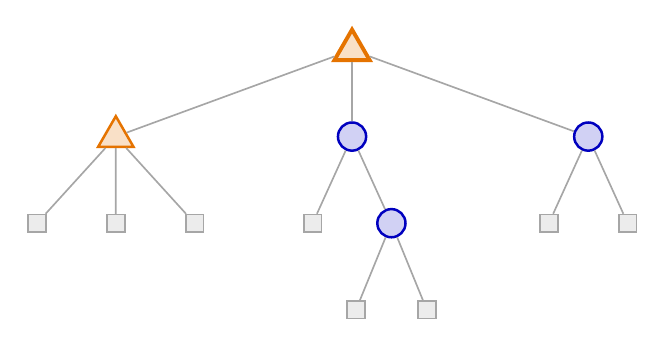
\begin{tikzpicture}[
  level distance=11mm,
  level 1/.style={sibling distance=30mm},
  level 2/.style={sibling distance=10mm},
  level 3/.style={sibling distance=9mm},
  T/.style={regular polygon,regular polygon sides=3,draw=cB,fill=cB!22,inner sep=2.6pt,line width=0.9pt},
  S/.style={circle,draw=cA,fill=cA!18,inner sep=3.6pt,line width=0.9pt},
  lf/.style={rectangle,draw=gray!70,fill=gray!15,inner sep=3.2pt},
  edge from parent/.style={draw=gray!70,line width=0.6pt}]
  \node[T,line width=1.4pt] {}
    child {node[T] {} child {node[lf] {}} child {node[lf] {}} child {node[lf] {}}}
    child {node[S] {} child {node[lf] {}} child {node[S] {} child {node[lf] {}} child {node[lf] {}}}}
    child {node[S] {} child {node[lf] {}} child {node[lf] {}}};
\end{tikzpicture}
\caption{圖~\ref{fig:root} 的分法對應的樹。三角形節點有 3 個小孩，圓形節點（弦）有 2 個小孩，
灰色方塊是葉子。共有 $5$ 個內部節點與 $8$ 片葉子。}
\label{fig:tree}
\end{figure}

\subsection{公式裡的 $L$ 是什麼}

式 \eqref{eq:gc} 裡的 $L=1+\sum_i n_i(v_i-1)$ 正好是這棵樹的\textbf{葉子數}。
理由：內部節點共 $b=\sum n_i$ 個，邊數是 $\sum n_iv_i=N$，而樹的「節點數 $=$ 邊數 $+1$」，
所以 $b+L=N+1$，即 $L=N+1-b$。圖~\ref{fig:tree} 中 $N=12$、$b=5$、$L=8$，吻合。

因此多項式係數 $\binom{N+1}{n_1,\ldots,n_k,L}$ 的意思是：
把 $N+1$ 個節點分成「各型內部節點」與「葉子」。

\subsection{Lagrange 反演}

原文最後的 Remark 指出：定理也可以直接對式 \eqref{eq:gf} 使用 Good 的多變數 Lagrange 反演公式得到。
Lagrange 反演的功能正是「由隱函數方程直接讀出係數」，所以可以跳過第三步的驗證，
直接從 $D=1+\sum_i x_iD^{v_i}$ 算出 $[x^{\vn}]D=\Cv(\vn)$。

\subsection{與不交叉分割（noncrossing partition）的關係}

用現代的語言，定理說的是：$\Cv(\vn)$ 是「各種大小的區塊數目給定」的不交叉分割的個數。
化簡後的公式 $\dfrac{N!}{\prod n_i!\,(N+1-b)!}$ 與 Kreweras (1972) 依區塊型別計數不交叉分割的結果一致。

% =====================================================================
\section{總結}
% =====================================================================

\begin{figure}[H]
\centering
\begin{tikzpicture}[
  box/.style={draw=blue!45!black,fill=blue!4,rounded corners=2pt,inner sep=5pt,align=center,font=\small,minimum width=7.2cm},
  arr/.style={-{Stealth[length=5pt]},line width=0.7pt,gray!60!black},
  node distance=4.2mm]
  \node[box] (a) {圓周上的 $N=\ip{\vn}{\vv}$ 個點};
  \node[box,below=of a] (b) {分成 $n_i$ 個 $v_i$ 點群組，互不交叉（凸多邊形）};
  \node[box,below=of b] (c) {固定一個點，看它所在的群組};
  \node[box,below=of c] (d) {其餘的點被切成 $v_i$ 段，各段獨立};
  \node[box,below=of d] (e) {遞迴：$d(\vn)=\sum_i\sum d(\vr_1)\cdots d(\vr_{v_i})$};
  \node[box,below=of e] (f) {生成函數：$D=1+\sum_i x_iD^{v_i}$};
  \node[box,below=of f] (g) {Raney 公式／Lagrange 反演};
  \node[box,below=of g,draw=orange!75!black,fill=orange!8] (h)
     {$d(\vn)=\Cv(\vn)=\dfrac{1}{N+1}\dbinom{N+1}{n_1,\ldots,n_k,\,L}$};
  \foreach \u/\w in {a/b,b/c,c/d,d/e,e/f,f/g,g/h}{\draw[arr] (\u)--(\w);}
\end{tikzpicture}
\caption{整篇論文的邏輯：幾何 $\to$ 遞迴分解 $\to$ 生成函數 $\to$ 閉式公式。}
\end{figure}

\subsection*{先備知識清單}
\begin{enumerate}
  \item 二項式係數與多項式係數。
  \item 經典卡塔蘭數，以及它的遞迴 $C_n=\sum_{j=0}^{n-1}C_jC_{n-1-j}$（「分成左右兩邊」的想法，第 1 節）。
  \item 不交叉的概念（圖~\ref{fig:catalan3}、圖~\ref{fig:crossing}）。
  \item 生成函數，以及「冪級數相乘 $=$ 係數做卷積」。
  \item 多變數生成函數只是多記幾個變數的帳，不需要多變數微積分。
  \item Raney 公式與 Lagrange 反演只在第三步用到。第一次讀可以先接受式 \eqref{eq:ct}，
        之後再讀第~\ref{sec:raney} 節的證明。
\end{enumerate}
讀懂到式 \eqref{eq:gf} 為止，就已經掌握這篇論文的核心想法。

\subsection*{符號表}
\begin{tabular}{@{}ll@{}}
\toprule
符號 & 意義\\
\midrule
$\vv=(v_1,\ldots,v_k)$ & 各型群組的點數\\
$\vn=(n_1,\ldots,n_k)$ & 各型群組的個數\\
$N=\ip{\vn}{\vv}$ & 圓周上的總點數 $\sum n_iv_i$\\
$b=\sum n_i$ & 群組總數\\
$L=1+\sum n_i(v_i-1)=N+1-b$ & 多項式係數的最後一格（樹的葉子數）\\
$\Cv(\vn)$ & 廣義卡塔蘭數（公式）\\
$d(\vn)$ & 不交叉分法的數目（要數的東西）\\
$\ve_i$ & 第 $i$ 個單位向量\\
$D(\vX)$、$C(\vX)$ & $d(\vn)$、$\Cv(\vn)$ 的生成函數\\
$[x^{\vn}]F$ & 冪級數 $F$ 中 $x_1^{n_1}\cdots x_k^{n_k}$ 的係數\\
\bottomrule
\end{tabular}

% =====================================================================
\appendix
\section{MIT 18.212 Lecture 1--4 補充（動畫 M01--M14）}\label{sec:mit}
% =====================================================================

這個附錄對應 manim 演示的 MIT 補充場景 M01--M14：小節 A.$k$ 對應場景 M$k$（兩位數編號）。
內容依據 MIT 18.212 Algebraic Combinatorics 的 Lecture 1--4（使用者提供的整理，見 \texttt{notes/MIT18212\_L1-4\_精簡.md}），
以〔MIT L1〕等標示講次。第 1 節已經講過的部分（Dyck 路徑、三角剖分與遞迴、反射原理、圓上配對、同一個 $C_n$）
這裡不再重複，只補第 1 節沒有的內容；它們都是第 1 節「根＋左＋右」結構的延伸，最後也回到 Chu 的方程。

\begin{center}
\small
\begin{tabular}{@{}lll@{\qquad}lll@{}}
\toprule
小節 & 內容 & 動畫 & 小節 & 內容 & 動畫\\
\midrule
A.1 & Cauchy 乘積 & M01 & A.8 & DFS：樹 → Dyck → 配對 & M08\\
A.2 & 生成函數的閉式 & M02 & A.9 & 堆疊與佇列排序 & M09\\
A.3 & 醉漢走路 & M03 & A.10 & 模式迴避 & M10\\
A.4 & 循環移位 & M04 & A.11 & 整數分割與 Young 表 & M11\\
A.5 & 平面樹 & M05 & A.12 & 標準 Young 表與 Dyck 路徑 & M12\\
A.6 & 弧圖：不交叉與不巢狀 & M06 & A.13 & 鉤長公式 & M13\\
A.7 & 三角剖分的對偶樹 & M07 & A.14 & 鉤上漫步的證明 & M14\\
\bottomrule
\end{tabular}
\end{center}

\begin{keybox}[貫穿的例子]
與圖~\ref{fig:onenumber} 的第 4 欄相同：五邊形三角剖分（對角線 $\{1,4\},\{2,4\}$）$\to$ 二元樹 $((\bullet,(\bullet,\bullet)),\bullet)$
$\to$ 平面樹（根 $\to$ A $\to$ 兩片葉子）$\to$ Dyck 路徑 UUDUDD $\to$ 配對 $(1,6),(2,3),(4,5)$
$\to$ 標準 Young 表 $\begin{smallmatrix}1&2&4\\3&5&6\end{smallmatrix}$；開票順序 AABABB、括號 $(a\cdot(b\cdot c))\cdot d$。
\end{keybox}

% figs_part1.tex —— 由 mit/make_figs_part1.py 產生，請勿手動修改。
% 重新產生：python mit/make_figs_part1.py（在 notes/ 裡）
\newcommand{\FigMiCauchy}{%
\begin{tikzpicture}
\node[font=\small,text=gray!70!black] at (0.625,0) {$\times$};
\node[font=\small,text=cRight] at (2.06,0) {$C_0$};
\node[font=\small,text=cRight] at (3.68,0) {$C_1x$};
\node[font=\small,text=cRight] at (5.3,0) {$C_2x^2$};
\node[font=\small,text=cRight] at (6.92,0) {$C_3x^3$};
\node[font=\small,text=cLeft] at (0.625,-0.78) {$C_0$};
\node[font=\small,text=cLeft] at (0.625,-1.56) {$C_1x$};
\node[font=\small,text=cLeft] at (0.625,-2.34) {$C_2x^2$};
\node[font=\small,text=cLeft] at (0.625,-3.12) {$C_3x^3$};
\fill[cA!9] (1.25,-1.17) rectangle (2.87,-0.39);
\node[font=\small] at (2.06,-0.65) {$\textcolor{cLeft}{C_0}\textcolor{cRight}{C_0}$};
\node[font=\scriptsize,text=gray!70!black] at (2.06,-0.97) {$=1$};
\fill[green!50!black!11] (2.87,-1.17) rectangle (4.49,-0.39);
\node[font=\small] at (3.68,-0.65) {$\textcolor{cLeft}{C_0}\textcolor{cRight}{C_1}x$};
\node[font=\scriptsize,text=gray!70!black] at (3.68,-0.97) {$=x$};
\fill[yellow!45] (4.49,-1.17) rectangle (6.11,-0.39);
\node[font=\small] at (5.3,-0.65) {$\textcolor{cLeft}{C_0}\textcolor{cRight}{C_2}x^2$};
\node[font=\scriptsize,text=gray!70!black] at (5.3,-0.97) {$=2x^2$};
\fill[orange!20] (6.11,-1.17) rectangle (7.73,-0.39);
\node[font=\small] at (6.92,-0.65) {$\textcolor{cLeft}{C_0}\textcolor{cRight}{C_3}x^3$};
\node[font=\scriptsize,text=gray!70!black] at (6.92,-0.97) {$=5x^3$};
\fill[green!50!black!11] (1.25,-1.95) rectangle (2.87,-1.17);
\node[font=\small] at (2.06,-1.43) {$\textcolor{cLeft}{C_1}\textcolor{cRight}{C_0}x$};
\node[font=\scriptsize,text=gray!70!black] at (2.06,-1.75) {$=x$};
\fill[yellow!45] (2.87,-1.95) rectangle (4.49,-1.17);
\node[font=\small] at (3.68,-1.43) {$\textcolor{cLeft}{C_1}\textcolor{cRight}{C_1}x^2$};
\node[font=\scriptsize,text=gray!70!black] at (3.68,-1.75) {$=x^2$};
\fill[orange!20] (4.49,-1.95) rectangle (6.11,-1.17);
\node[font=\small] at (5.3,-1.43) {$\textcolor{cLeft}{C_1}\textcolor{cRight}{C_2}x^3$};
\node[font=\scriptsize,text=gray!70!black] at (5.3,-1.75) {$=2x^3$};
\node[font=\small,text=gray!55] at (6.92,-1.43) {$C_1C_3x^4$};
\node[font=\scriptsize,text=gray!55] at (6.92,-1.75) {$=5x^4$};
\fill[yellow!45] (1.25,-2.73) rectangle (2.87,-1.95);
\node[font=\small] at (2.06,-2.21) {$\textcolor{cLeft}{C_2}\textcolor{cRight}{C_0}x^2$};
\node[font=\scriptsize,text=gray!70!black] at (2.06,-2.53) {$=2x^2$};
\fill[orange!20] (2.87,-2.73) rectangle (4.49,-1.95);
\node[font=\small] at (3.68,-2.21) {$\textcolor{cLeft}{C_2}\textcolor{cRight}{C_1}x^3$};
\node[font=\scriptsize,text=gray!70!black] at (3.68,-2.53) {$=2x^3$};
\node[font=\small,text=gray!55] at (5.3,-2.21) {$C_2C_2x^4$};
\node[font=\scriptsize,text=gray!55] at (5.3,-2.53) {$=4x^4$};
\node[font=\small,text=gray!55] at (6.92,-2.21) {$C_2C_3x^5$};
\node[font=\scriptsize,text=gray!55] at (6.92,-2.53) {$=10x^5$};
\fill[orange!20] (1.25,-3.51) rectangle (2.87,-2.73);
\node[font=\small] at (2.06,-2.99) {$\textcolor{cLeft}{C_3}\textcolor{cRight}{C_0}x^3$};
\node[font=\scriptsize,text=gray!70!black] at (2.06,-3.31) {$=5x^3$};
\node[font=\small,text=gray!55] at (3.68,-2.99) {$C_3C_1x^4$};
\node[font=\scriptsize,text=gray!55] at (3.68,-3.31) {$=5x^4$};
\node[font=\small,text=gray!55] at (5.3,-2.99) {$C_3C_2x^5$};
\node[font=\scriptsize,text=gray!55] at (5.3,-3.31) {$=10x^5$};
\node[font=\small,text=gray!55] at (6.92,-2.99) {$C_3C_3x^6$};
\node[font=\scriptsize,text=gray!55] at (6.92,-3.31) {$=25x^6$};
\draw[gray!55,line width=0.4pt] (1.25,-0.39) -- (7.73,-0.39);
\draw[gray!55,line width=0.4pt] (1.25,-1.17) -- (7.73,-1.17);
\draw[gray!55,line width=0.4pt] (1.25,-1.95) -- (7.73,-1.95);
\draw[gray!55,line width=0.4pt] (1.25,-2.73) -- (7.73,-2.73);
\draw[gray!55,line width=0.4pt] (1.25,-3.51) -- (7.73,-3.51);
\draw[gray!55,line width=0.4pt] (1.25,-0.39) -- (1.25,-3.51);
\draw[gray!55,line width=0.4pt] (2.87,-0.39) -- (2.87,-3.51);
\draw[gray!55,line width=0.4pt] (4.49,-0.39) -- (4.49,-3.51);
\draw[gray!55,line width=0.4pt] (6.11,-0.39) -- (6.11,-3.51);
\draw[gray!55,line width=0.4pt] (7.73,-0.39) -- (7.73,-3.51);
\fill[cA!9] (8.48,-0.95) rectangle (8.82,-0.61);
\draw[gray!55,line width=0.3pt] (8.48,-0.95) rectangle (8.82,-0.61);
\node[anchor=west,font=\small] at (8.98,-0.78) {$[x^0]\,C^2=1$};
\fill[green!50!black!11] (8.48,-1.73) rectangle (8.82,-1.39);
\draw[gray!55,line width=0.3pt] (8.48,-1.73) rectangle (8.82,-1.39);
\node[anchor=west,font=\small] at (8.98,-1.56) {$[x]\,C^2=1+1=2$};
\fill[yellow!45] (8.48,-2.51) rectangle (8.82,-2.17);
\draw[gray!55,line width=0.3pt] (8.48,-2.51) rectangle (8.82,-2.17);
\node[anchor=west,font=\small] at (8.98,-2.34) {$[x^2]\,C^2=2+1+2=5$};
\fill[orange!20] (8.48,-3.29) rectangle (8.82,-2.95);
\draw[gray!55,line width=0.3pt] (8.48,-3.29) rectangle (8.82,-2.95);
\node[anchor=west,font=\small] at (8.98,-3.12) {$[x^3]\,C^2=5+2+2+5=14$};
\node[anchor=west,font=\footnotesize,text=gray!70!black] at (8.48,0) {同色的格子加起來：};
\end{tikzpicture}}
\newcommand{\FigMiiBranches}{%
\begin{tikzpicture}
\draw[-{Stealth[length=4pt]},gray!70!black,line width=0.5pt] (0,0) -- (4.2,0) node[right,font=\small] {$x$};
\draw[-{Stealth[length=4pt]},gray!70!black,line width=0.5pt] (0,0) -- (0,2.85);
\draw[gray!45,dashed,line width=0.4pt] (3.75,0) -- (3.75,1);
\node[below,font=\small] at (3.75,0) {$\frac14$};
\node[below left,font=\small] at (0,0) {$0$};
\draw[gray!70!black,line width=0.4pt] (-0.07,0.5) -- (0.07,0.5);
\node[left,font=\scriptsize] at (-0.07,0.5) {$1$};
\draw[gray!70!black,line width=0.4pt] (-0.07,1) -- (0.07,1);
\node[left,font=\scriptsize] at (-0.07,1) {$2$};
\draw[gray!70!black,line width=0.4pt] (-0.07,1.5) -- (0.07,1.5);
\node[left,font=\scriptsize] at (-0.07,1.5) {$3$};
\draw[gray!70!black,line width=0.4pt] (-0.07,2) -- (0.07,2);
\node[left,font=\scriptsize] at (-0.07,2) {$4$};
\draw[gray!70!black,line width=0.4pt] (-0.07,2.5) -- (0.07,2.5);
\node[left,font=\scriptsize] at (-0.07,2.5) {$5$};
\draw[cA,line width=1.3pt] (0,0.5) -- (0.037,0.501) -- (0.075,0.503) -- (0.112,0.504) -- (0.15,0.505) -- (0.188,0.506) -- (0.225,0.508) -- (0.263,0.509) -- (0.3,0.51) -- (0.337,0.512) -- (0.375,0.513) -- (0.412,0.515) -- (0.45,0.516) -- (0.488,0.517) -- (0.525,0.519) -- (0.562,0.52) -- (0.6,0.522) -- (0.638,0.523) -- (0.675,0.525) -- (0.713,0.526) -- (0.75,0.528) -- (0.787,0.529) -- (0.825,0.531) -- (0.863,0.533) -- (0.9,0.534) -- (0.938,0.536) -- (0.975,0.538) -- (1.013,0.539) -- (1.05,0.541) -- (1.087,0.543) -- (1.125,0.544) -- (1.163,0.546) -- (1.2,0.548) -- (1.238,0.55) -- (1.275,0.552) -- (1.313,0.554) -- (1.35,0.556) -- (1.387,0.557) -- (1.425,0.559) -- (1.463,0.561) -- (1.5,0.564) -- (1.538,0.566) -- (1.575,0.568) -- (1.613,0.57) -- (1.65,0.572) -- (1.688,0.574) -- (1.725,0.576) -- (1.763,0.579) -- (1.8,0.581) -- (1.837,0.583) -- (1.875,0.586) -- (1.913,0.588) -- (1.95,0.591) -- (1.988,0.593) -- (2.025,0.596) -- (2.062,0.599) -- (2.1,0.601) -- (2.138,0.604) -- (2.175,0.607) -- (2.212,0.61) -- (2.25,0.613) -- (2.288,0.616) -- (2.325,0.619) -- (2.362,0.622) -- (2.4,0.625) -- (2.438,0.628) -- (2.475,0.632) -- (2.513,0.635) -- (2.55,0.639) -- (2.588,0.642) -- (2.625,0.646) -- (2.662,0.65) -- (2.7,0.654) -- (2.737,0.658) -- (2.775,0.662) -- (2.812,0.667) -- (2.85,0.671) -- (2.888,0.676) -- (2.925,0.681) -- (2.963,0.686) -- (3,0.691) -- (3.038,0.696) -- (3.075,0.702) -- (3.113,0.708) -- (3.15,0.714) -- (3.188,0.721) -- (3.225,0.728) -- (3.263,0.735) -- (3.3,0.743) -- (3.337,0.751) -- (3.375,0.76) -- (3.413,0.769) -- (3.45,0.78) -- (3.488,0.791) -- (3.525,0.803) -- (3.563,0.817) -- (3.6,0.833) -- (3.637,0.852) -- (3.675,0.876) -- (3.712,0.909) -- (3.75,1);
\draw[cBad,line width=1.3pt] (2.4,2.5) -- (2.415,2.479) -- (2.43,2.459) -- (2.445,2.439) -- (2.46,2.418) -- (2.475,2.399) -- (2.49,2.379) -- (2.505,2.36) -- (2.52,2.34) -- (2.535,2.321) -- (2.55,2.302) -- (2.565,2.284) -- (2.58,2.265) -- (2.595,2.247) -- (2.61,2.229) -- (2.625,2.211) -- (2.64,2.193) -- (2.655,2.176) -- (2.67,2.158) -- (2.685,2.141) -- (2.7,2.124) -- (2.715,2.107) -- (2.73,2.09) -- (2.745,2.073) -- (2.76,2.057) -- (2.775,2.04) -- (2.79,2.024) -- (2.805,2.008) -- (2.82,1.992) -- (2.835,1.976) -- (2.85,1.96) -- (2.865,1.945) -- (2.88,1.929) -- (2.895,1.914) -- (2.91,1.899) -- (2.925,1.883) -- (2.94,1.868) -- (2.955,1.853) -- (2.97,1.838) -- (2.985,1.824) -- (3,1.809) -- (3.015,1.794) -- (3.03,1.78) -- (3.045,1.766) -- (3.06,1.751) -- (3.075,1.737) -- (3.09,1.723) -- (3.105,1.709) -- (3.12,1.695) -- (3.135,1.681) -- (3.15,1.667) -- (3.165,1.653) -- (3.18,1.639) -- (3.195,1.625) -- (3.21,1.612) -- (3.225,1.598) -- (3.24,1.584) -- (3.255,1.571) -- (3.27,1.557) -- (3.285,1.544) -- (3.3,1.53) -- (3.315,1.517) -- (3.33,1.503) -- (3.345,1.489) -- (3.36,1.476) -- (3.375,1.462) -- (3.39,1.449) -- (3.405,1.435) -- (3.42,1.422) -- (3.435,1.408) -- (3.45,1.394) -- (3.465,1.381) -- (3.48,1.367) -- (3.495,1.353) -- (3.51,1.339) -- (3.525,1.324) -- (3.54,1.31) -- (3.555,1.295) -- (3.57,1.281) -- (3.585,1.265) -- (3.6,1.25) -- (3.615,1.234) -- (3.63,1.218) -- (3.645,1.201) -- (3.66,1.183) -- (3.675,1.165) -- (3.69,1.145) -- (3.705,1.123) -- (3.72,1.098) -- (3.735,1.068) -- (3.75,1);
\draw[-{Stealth[length=5pt]},cBad,line width=1.3pt] (2.4,2.5) -- (2.22,2.768);
\fill[cA] (0,0.5) circle (0.07);
\fill[black] (3.75,1) circle (0.05);
\node[anchor=north west,font=\scriptsize,text=cA] at (0.04,0.46) {$C(0)=C_0=1$};
\node[right,font=\scriptsize,text=cBad] at (2.475,2.375) {取 $+$：$x\to0$ 時 $\to\infty$};
\node[above,font=\scriptsize,text=cA] at (1.95,0.641) {取 $-$};
\node[right,font=\scriptsize] at (3.8,1.12) {$(\frac14,2)$};
\end{tikzpicture}}
\newcommand{\FigMiiiWalk}{%
\begin{tikzpicture}
\draw[gray!22,line width=0.3pt] (0,0.42) -- (3.74,0.42);
\draw[gray!22,line width=0.3pt] (0,0.84) -- (3.74,0.84);
\draw[gray!60,line width=0.5pt] (0,0) -- (3.74,0);
\draw[cBad,dashed,line width=0.6pt] (0,-0.42) -- (3.74,-0.42) node[right,font=\scriptsize,text=cBad] {懸崖};
\draw[-{Stealth[length=4pt]},gray!70!black,line width=0.5pt] (0,-0.672) -- (0,1.26) node[above,font=\scriptsize] {位置};
\node[font=\scriptsize,text=gray!70!black] at (1.82,-1.155) {時間（步數）$\to$};
\node[left,font=\scriptsize,text=cBad] at (-0.02,-0.42) {$-1$};
\node[left,font=\scriptsize,text=black] at (-0.02,0) {$0$};
\node[left,font=\scriptsize,text=black] at (-0.02,0.42) {$1$};
\node[left,font=\scriptsize,text=black] at (-0.02,0.84) {$2$};
\draw[cA,line width=1.5pt,line cap=round] (0,0) -- (0.52,0.42);
\draw[cA,line width=1.5pt,line cap=round] (0.52,0.42) -- (1.04,0.84);
\draw[cA,line width=1.5pt,line cap=round] (1.04,0.84) -- (1.56,0.42);
\draw[cA,line width=1.5pt,line cap=round] (1.56,0.42) -- (2.08,0.84);
\draw[cA,line width=1.5pt,line cap=round] (2.08,0.84) -- (2.6,0.42);
\draw[cA,line width=1.5pt,line cap=round] (2.6,0.42) -- (3.12,0);
\draw[cBad,line width=1.5pt,line cap=round] (3.12,0) -- (3.64,-0.42);
\fill[black!70] (0,0) circle (0.035);
\fill[black!70] (0.52,0.42) circle (0.035);
\fill[black!70] (1.04,0.84) circle (0.035);
\fill[black!70] (1.56,0.42) circle (0.035);
\fill[black!70] (2.08,0.84) circle (0.035);
\fill[black!70] (2.6,0.42) circle (0.035);
\fill[black!70] (3.12,0) circle (0.035);
\fill[black!70] (3.64,-0.42) circle (0.035);
\fill[cBad] (3.64,-0.42) circle (0.07);
\node[font=\scriptsize,text=cA] at (0.26,-0.777) {$\mathrm{U}$};
\node[font=\scriptsize,text=cA] at (0.78,-0.777) {$\mathrm{U}$};
\node[font=\scriptsize,text=cA] at (1.3,-0.777) {$\mathrm{D}$};
\node[font=\scriptsize,text=cA] at (1.82,-0.777) {$\mathrm{U}$};
\node[font=\scriptsize,text=cA] at (2.34,-0.777) {$\mathrm{D}$};
\node[font=\scriptsize,text=cA] at (2.86,-0.777) {$\mathrm{D}$};
\node[font=\scriptsize,text=cBad] at (3.38,-0.777) {$\mathrm{D}$};
\node[font=\small] at (5.4,1.05) {$n=0$};
\draw[gray!55,line width=0.3pt] (5.32,0.4) -- (5.48,0.4);
\draw[cBad!70,dashed,line width=0.3pt] (5.32,0.24) -- (5.48,0.24);
\draw[cBad,line width=1.1pt,line cap=round] (5.32,0.4) -- (5.48,0.24);
\node[font=\small] at (5.4,-1) {$1$ 條};
\node[font=\small] at (5.4,-1.6) {$\frac{1}{2}$};
\node[font=\small] at (6.65,1.05) {$n=1$};
\draw[gray!55,line width=0.3pt] (6.41,0.4) -- (6.89,0.4);
\draw[cBad!70,dashed,line width=0.3pt] (6.41,0.24) -- (6.89,0.24);
\draw[cA,line width=1.1pt,line cap=round] (6.41,0.4) -- (6.57,0.56);
\draw[cA,line width=1.1pt,line cap=round] (6.57,0.56) -- (6.73,0.4);
\draw[cBad,line width=1.1pt,line cap=round] (6.73,0.4) -- (6.89,0.24);
\node[font=\small] at (6.65,-1) {$1$ 條};
\node[font=\small] at (6.65,-1.6) {$\frac{1}{8}$};
\node[font=\small] at (8.55,1.05) {$n=2$};
\draw[gray!55,line width=0.3pt] (7.64,0.4) -- (8.44,0.4);
\draw[cBad!70,dashed,line width=0.3pt] (7.64,0.24) -- (8.44,0.24);
\draw[cA,line width=1.1pt,line cap=round] (7.64,0.4) -- (7.8,0.56);
\draw[cA,line width=1.1pt,line cap=round] (7.8,0.56) -- (7.96,0.4);
\draw[cA,line width=1.1pt,line cap=round] (7.96,0.4) -- (8.12,0.56);
\draw[cA,line width=1.1pt,line cap=round] (8.12,0.56) -- (8.28,0.4);
\draw[cBad,line width=1.1pt,line cap=round] (8.28,0.4) -- (8.44,0.24);
\draw[gray!55,line width=0.3pt] (8.66,0.4) -- (9.46,0.4);
\draw[cBad!70,dashed,line width=0.3pt] (8.66,0.24) -- (9.46,0.24);
\draw[cA,line width=1.1pt,line cap=round] (8.66,0.4) -- (8.82,0.56);
\draw[cA,line width=1.1pt,line cap=round] (8.82,0.56) -- (8.98,0.72);
\draw[cA,line width=1.1pt,line cap=round] (8.98,0.72) -- (9.14,0.56);
\draw[cA,line width=1.1pt,line cap=round] (9.14,0.56) -- (9.3,0.4);
\draw[cBad,line width=1.1pt,line cap=round] (9.3,0.4) -- (9.46,0.24);
\node[font=\small] at (8.55,-1) {$2$ 條};
\node[font=\small] at (8.55,-1.6) {$\frac{2}{32}$};
\node[font=\small] at (12.11,1.05) {$n=3$};
\draw[gray!55,line width=0.3pt] (10.21,0.4) -- (11.33,0.4);
\draw[cBad!70,dashed,line width=0.3pt] (10.21,0.24) -- (11.33,0.24);
\draw[cA,line width=1.1pt,line cap=round] (10.21,0.4) -- (10.37,0.56);
\draw[cA,line width=1.1pt,line cap=round] (10.37,0.56) -- (10.53,0.4);
\draw[cA,line width=1.1pt,line cap=round] (10.53,0.4) -- (10.69,0.56);
\draw[cA,line width=1.1pt,line cap=round] (10.69,0.56) -- (10.85,0.4);
\draw[cA,line width=1.1pt,line cap=round] (10.85,0.4) -- (11.01,0.56);
\draw[cA,line width=1.1pt,line cap=round] (11.01,0.56) -- (11.17,0.4);
\draw[cBad,line width=1.1pt,line cap=round] (11.17,0.4) -- (11.33,0.24);
\draw[gray!55,line width=0.3pt] (11.55,0.4) -- (12.67,0.4);
\draw[cBad!70,dashed,line width=0.3pt] (11.55,0.24) -- (12.67,0.24);
\draw[cA,line width=1.1pt,line cap=round] (11.55,0.4) -- (11.71,0.56);
\draw[cA,line width=1.1pt,line cap=round] (11.71,0.56) -- (11.87,0.4);
\draw[cA,line width=1.1pt,line cap=round] (11.87,0.4) -- (12.03,0.56);
\draw[cA,line width=1.1pt,line cap=round] (12.03,0.56) -- (12.19,0.72);
\draw[cA,line width=1.1pt,line cap=round] (12.19,0.72) -- (12.35,0.56);
\draw[cA,line width=1.1pt,line cap=round] (12.35,0.56) -- (12.51,0.4);
\draw[cBad,line width=1.1pt,line cap=round] (12.51,0.4) -- (12.67,0.24);
\draw[gray!55,line width=0.3pt] (12.89,0.4) -- (14.01,0.4);
\draw[cBad!70,dashed,line width=0.3pt] (12.89,0.24) -- (14.01,0.24);
\draw[cA,line width=1.1pt,line cap=round] (12.89,0.4) -- (13.05,0.56);
\draw[cA,line width=1.1pt,line cap=round] (13.05,0.56) -- (13.21,0.72);
\draw[cA,line width=1.1pt,line cap=round] (13.21,0.72) -- (13.37,0.56);
\draw[cA,line width=1.1pt,line cap=round] (13.37,0.56) -- (13.53,0.4);
\draw[cA,line width=1.1pt,line cap=round] (13.53,0.4) -- (13.69,0.56);
\draw[cA,line width=1.1pt,line cap=round] (13.69,0.56) -- (13.85,0.4);
\draw[cBad,line width=1.1pt,line cap=round] (13.85,0.4) -- (14.01,0.24);
\draw[cA!60,rounded corners=1.5pt,line width=0.5pt] (10.8,-0.74) rectangle (12.08,-0.1);
\draw[gray!55,line width=0.3pt] (10.88,-0.5) -- (12,-0.5);
\draw[cBad!70,dashed,line width=0.3pt] (10.88,-0.66) -- (12,-0.66);
\draw[cA,line width=1.1pt,line cap=round] (10.88,-0.5) -- (11.04,-0.34);
\draw[cA,line width=1.1pt,line cap=round] (11.04,-0.34) -- (11.2,-0.18);
\draw[cA,line width=1.1pt,line cap=round] (11.2,-0.18) -- (11.36,-0.34);
\draw[cA,line width=1.1pt,line cap=round] (11.36,-0.34) -- (11.52,-0.18);
\draw[cA,line width=1.1pt,line cap=round] (11.52,-0.18) -- (11.68,-0.34);
\draw[cA,line width=1.1pt,line cap=round] (11.68,-0.34) -- (11.84,-0.5);
\draw[cBad,line width=1.1pt,line cap=round] (11.84,-0.5) -- (12,-0.66);
\draw[gray!55,line width=0.3pt] (12.22,-0.5) -- (13.34,-0.5);
\draw[cBad!70,dashed,line width=0.3pt] (12.22,-0.66) -- (13.34,-0.66);
\draw[cA,line width=1.1pt,line cap=round] (12.22,-0.5) -- (12.38,-0.34);
\draw[cA,line width=1.1pt,line cap=round] (12.38,-0.34) -- (12.54,-0.18);
\draw[cA,line width=1.1pt,line cap=round] (12.54,-0.18) -- (12.7,-0.02);
\draw[cA,line width=1.1pt,line cap=round] (12.7,-0.02) -- (12.86,-0.18);
\draw[cA,line width=1.1pt,line cap=round] (12.86,-0.18) -- (13.02,-0.34);
\draw[cA,line width=1.1pt,line cap=round] (13.02,-0.34) -- (13.18,-0.5);
\draw[cBad,line width=1.1pt,line cap=round] (13.18,-0.5) -- (13.34,-0.66);
\node[font=\small] at (12.11,-1) {$5$ 條};
\node[font=\small] at (12.11,-1.6) {$\frac{5}{128}$};
\node[anchor=east,font=\scriptsize,text=gray!70!black] at (5,0.4) {走法};
\node[anchor=east,font=\scriptsize,text=gray!70!black] at (5,-1) {條數};
\node[anchor=east,font=\scriptsize,text=gray!70!black] at (5,-1.6) {機率};
\end{tikzpicture}}
\newcommand{\FigMivRotations}{%
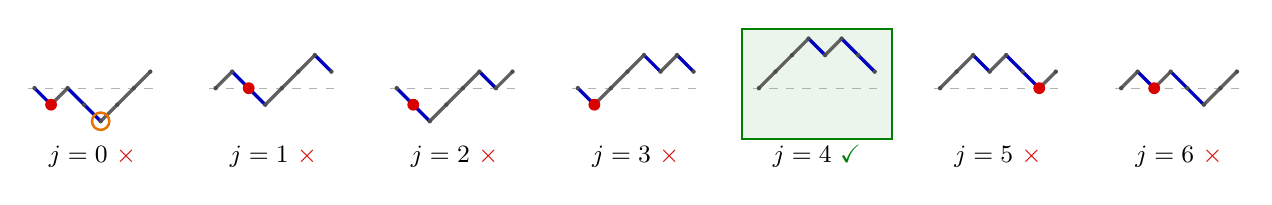
\begin{tikzpicture}
\draw[gray!60,dashed,line width=0.4pt] (-0.08,0) -- (1.55,0);
\draw[cA,line width=1.2pt,line cap=round] (0,0) -- (0.21,-0.21);
\draw[gray!75!black,line width=1.2pt,line cap=round] (0.21,-0.21) -- (0.42,0);
\draw[cA,line width=1.2pt,line cap=round] (0.42,0) -- (0.63,-0.21);
\draw[cA,line width=1.2pt,line cap=round] (0.63,-0.21) -- (0.84,-0.42);
\draw[gray!75!black,line width=1.2pt,line cap=round] (0.84,-0.42) -- (1.05,-0.21);
\draw[gray!75!black,line width=1.2pt,line cap=round] (1.05,-0.21) -- (1.26,0);
\draw[gray!75!black,line width=1.2pt,line cap=round] (1.26,0) -- (1.47,0.21);
\fill[black!70] (0,0) circle (0.028);
\fill[black!70] (0.21,-0.21) circle (0.028);
\fill[black!70] (0.42,0) circle (0.028);
\fill[black!70] (0.63,-0.21) circle (0.028);
\fill[black!70] (0.84,-0.42) circle (0.028);
\fill[black!70] (1.05,-0.21) circle (0.028);
\fill[black!70] (1.26,0) circle (0.028);
\fill[black!70] (1.47,0.21) circle (0.028);
\fill[cBad] (0.21,-0.21) circle (0.075);
\draw[cTop,line width=0.9pt] (0.84,-0.42) circle (0.11);
\node[font=\small] at (0.735,-0.865) {$j=0$\ \textcolor{cBad}{$\times$}};
\draw[gray!60,dashed,line width=0.4pt] (2.22,0) -- (3.85,0);
\draw[gray!75!black,line width=1.2pt,line cap=round] (2.3,0) -- (2.51,0.21);
\draw[cA,line width=1.2pt,line cap=round] (2.51,0.21) -- (2.72,0);
\draw[cA,line width=1.2pt,line cap=round] (2.72,0) -- (2.93,-0.21);
\draw[gray!75!black,line width=1.2pt,line cap=round] (2.93,-0.21) -- (3.14,0);
\draw[gray!75!black,line width=1.2pt,line cap=round] (3.14,0) -- (3.35,0.21);
\draw[gray!75!black,line width=1.2pt,line cap=round] (3.35,0.21) -- (3.56,0.42);
\draw[cA,line width=1.2pt,line cap=round] (3.56,0.42) -- (3.77,0.21);
\fill[black!70] (2.3,0) circle (0.028);
\fill[black!70] (2.51,0.21) circle (0.028);
\fill[black!70] (2.72,0) circle (0.028);
\fill[black!70] (2.93,-0.21) circle (0.028);
\fill[black!70] (3.14,0) circle (0.028);
\fill[black!70] (3.35,0.21) circle (0.028);
\fill[black!70] (3.56,0.42) circle (0.028);
\fill[black!70] (3.77,0.21) circle (0.028);
\fill[cBad] (2.72,0) circle (0.075);
\node[font=\small] at (3.035,-0.865) {$j=1$\ \textcolor{cBad}{$\times$}};
\draw[gray!60,dashed,line width=0.4pt] (4.52,0) -- (6.15,0);
\draw[cA,line width=1.2pt,line cap=round] (4.6,0) -- (4.81,-0.21);
\draw[cA,line width=1.2pt,line cap=round] (4.81,-0.21) -- (5.02,-0.42);
\draw[gray!75!black,line width=1.2pt,line cap=round] (5.02,-0.42) -- (5.23,-0.21);
\draw[gray!75!black,line width=1.2pt,line cap=round] (5.23,-0.21) -- (5.44,0);
\draw[gray!75!black,line width=1.2pt,line cap=round] (5.44,0) -- (5.65,0.21);
\draw[cA,line width=1.2pt,line cap=round] (5.65,0.21) -- (5.86,0);
\draw[gray!75!black,line width=1.2pt,line cap=round] (5.86,0) -- (6.07,0.21);
\fill[black!70] (4.6,0) circle (0.028);
\fill[black!70] (4.81,-0.21) circle (0.028);
\fill[black!70] (5.02,-0.42) circle (0.028);
\fill[black!70] (5.23,-0.21) circle (0.028);
\fill[black!70] (5.44,0) circle (0.028);
\fill[black!70] (5.65,0.21) circle (0.028);
\fill[black!70] (5.86,0) circle (0.028);
\fill[black!70] (6.07,0.21) circle (0.028);
\fill[cBad] (4.81,-0.21) circle (0.075);
\node[font=\small] at (5.335,-0.865) {$j=2$\ \textcolor{cBad}{$\times$}};
\draw[gray!60,dashed,line width=0.4pt] (6.82,0) -- (8.45,0);
\draw[cA,line width=1.2pt,line cap=round] (6.9,0) -- (7.11,-0.21);
\draw[gray!75!black,line width=1.2pt,line cap=round] (7.11,-0.21) -- (7.32,0);
\draw[gray!75!black,line width=1.2pt,line cap=round] (7.32,0) -- (7.53,0.21);
\draw[gray!75!black,line width=1.2pt,line cap=round] (7.53,0.21) -- (7.74,0.42);
\draw[cA,line width=1.2pt,line cap=round] (7.74,0.42) -- (7.95,0.21);
\draw[gray!75!black,line width=1.2pt,line cap=round] (7.95,0.21) -- (8.16,0.42);
\draw[cA,line width=1.2pt,line cap=round] (8.16,0.42) -- (8.37,0.21);
\fill[black!70] (6.9,0) circle (0.028);
\fill[black!70] (7.11,-0.21) circle (0.028);
\fill[black!70] (7.32,0) circle (0.028);
\fill[black!70] (7.53,0.21) circle (0.028);
\fill[black!70] (7.74,0.42) circle (0.028);
\fill[black!70] (7.95,0.21) circle (0.028);
\fill[black!70] (8.16,0.42) circle (0.028);
\fill[black!70] (8.37,0.21) circle (0.028);
\fill[cBad] (7.11,-0.21) circle (0.075);
\node[font=\small] at (7.635,-0.865) {$j=3$\ \textcolor{cBad}{$\times$}};
\fill[green!50!black!8] (8.98,-0.64) rectangle (10.89,0.756);
\draw[green!50!black,line width=0.7pt] (8.98,-0.64) rectangle (10.89,0.756);
\draw[gray!60,dashed,line width=0.4pt] (9.12,0) -- (10.75,0);
\draw[gray!75!black,line width=1.2pt,line cap=round] (9.2,0) -- (9.41,0.21);
\draw[gray!75!black,line width=1.2pt,line cap=round] (9.41,0.21) -- (9.62,0.42);
\draw[gray!75!black,line width=1.2pt,line cap=round] (9.62,0.42) -- (9.83,0.63);
\draw[cA,line width=1.2pt,line cap=round] (9.83,0.63) -- (10.04,0.42);
\draw[gray!75!black,line width=1.2pt,line cap=round] (10.04,0.42) -- (10.25,0.63);
\draw[cA,line width=1.2pt,line cap=round] (10.25,0.63) -- (10.46,0.42);
\draw[cA,line width=1.2pt,line cap=round] (10.46,0.42) -- (10.67,0.21);
\fill[black!70] (9.2,0) circle (0.028);
\fill[black!70] (9.41,0.21) circle (0.028);
\fill[black!70] (9.62,0.42) circle (0.028);
\fill[black!70] (9.83,0.63) circle (0.028);
\fill[black!70] (10.04,0.42) circle (0.028);
\fill[black!70] (10.25,0.63) circle (0.028);
\fill[black!70] (10.46,0.42) circle (0.028);
\fill[black!70] (10.67,0.21) circle (0.028);
\node[font=\small] at (9.935,-0.865) {$j=4$\ \textcolor{green!50!black}{\checkmark}};
\draw[gray!60,dashed,line width=0.4pt] (11.42,0) -- (13.05,0);
\draw[gray!75!black,line width=1.2pt,line cap=round] (11.5,0) -- (11.71,0.21);
\draw[gray!75!black,line width=1.2pt,line cap=round] (11.71,0.21) -- (11.92,0.42);
\draw[cA,line width=1.2pt,line cap=round] (11.92,0.42) -- (12.13,0.21);
\draw[gray!75!black,line width=1.2pt,line cap=round] (12.13,0.21) -- (12.34,0.42);
\draw[cA,line width=1.2pt,line cap=round] (12.34,0.42) -- (12.55,0.21);
\draw[cA,line width=1.2pt,line cap=round] (12.55,0.21) -- (12.76,0);
\draw[gray!75!black,line width=1.2pt,line cap=round] (12.76,0) -- (12.97,0.21);
\fill[black!70] (11.5,0) circle (0.028);
\fill[black!70] (11.71,0.21) circle (0.028);
\fill[black!70] (11.92,0.42) circle (0.028);
\fill[black!70] (12.13,0.21) circle (0.028);
\fill[black!70] (12.34,0.42) circle (0.028);
\fill[black!70] (12.55,0.21) circle (0.028);
\fill[black!70] (12.76,0) circle (0.028);
\fill[black!70] (12.97,0.21) circle (0.028);
\fill[cBad] (12.76,0) circle (0.075);
\node[font=\small] at (12.235,-0.865) {$j=5$\ \textcolor{cBad}{$\times$}};
\draw[gray!60,dashed,line width=0.4pt] (13.72,0) -- (15.35,0);
\draw[gray!75!black,line width=1.2pt,line cap=round] (13.8,0) -- (14.01,0.21);
\draw[cA,line width=1.2pt,line cap=round] (14.01,0.21) -- (14.22,0);
\draw[gray!75!black,line width=1.2pt,line cap=round] (14.22,0) -- (14.43,0.21);
\draw[cA,line width=1.2pt,line cap=round] (14.43,0.21) -- (14.64,0);
\draw[cA,line width=1.2pt,line cap=round] (14.64,0) -- (14.85,-0.21);
\draw[gray!75!black,line width=1.2pt,line cap=round] (14.85,-0.21) -- (15.06,0);
\draw[gray!75!black,line width=1.2pt,line cap=round] (15.06,0) -- (15.27,0.21);
\fill[black!70] (13.8,0) circle (0.028);
\fill[black!70] (14.01,0.21) circle (0.028);
\fill[black!70] (14.22,0) circle (0.028);
\fill[black!70] (14.43,0.21) circle (0.028);
\fill[black!70] (14.64,0) circle (0.028);
\fill[black!70] (14.85,-0.21) circle (0.028);
\fill[black!70] (15.06,0) circle (0.028);
\fill[black!70] (15.27,0.21) circle (0.028);
\fill[cBad] (14.22,0) circle (0.075);
\node[font=\small] at (14.535,-0.865) {$j=6$\ \textcolor{cBad}{$\times$}};
\end{tikzpicture}}

% =====================================================================
% 附錄 A 第 1 段：A.1–A.4（動畫 M01–M04）
% 圖由 mit/make_figs_part1.py 產生（含數字檢查），請勿手改 mit/figs_part1.tex
% =====================================================================

% ---------------------------------------------------------------------
\subsection{Cauchy 乘積}\label{sec:m01}

第 1.12 節把「根＋左＋右」直接翻譯成 $C=1+xC^2$。這一小節把中間的關鍵一步看清楚：
為什麼「左、右互相獨立」在代數上就是「生成函數相乘」\mitref{L1}。

\textbf{冪級數的乘法。}設 $A(x)=\sum_n a_nx^n$、$B(x)=\sum_n b_nx^n$。相乘時
$a_kx^k$ 和 $b_{n-k}x^{n-k}$ 的乘積正好落在 $x^n$，所以
\begin{equation}\label{eq:m01-cauchy}
[x^n]\,(A\cdot B)=\sum_{k=0}^{n}a_k\,b_{n-k}=a_0b_n+a_1b_{n-1}+\cdots+a_nb_0 .
\end{equation}
這叫做 \textbf{Cauchy 乘積}。排成乘法表最清楚：第 $i$ 列放 $a_ix^i$、第 $j$ 行放 $b_jx^j$，
格子 $(i,j)$ 放 $a_ib_j\,x^{i+j}$。次方相同的格子都在同一條反對角線 $i+j=n$ 上，
$[x^n]$ 就是把這條反對角線上的格子加起來。例如 $x^2$ 的係數（圖~\ref{fig:m01-table} 的黃色格子）是
$\textcolor{cLeft}{C_0}\textcolor{cRight}{C_2}+\textcolor{cLeft}{C_1}\textcolor{cRight}{C_1}
+\textcolor{cLeft}{C_2}\textcolor{cRight}{C_0}=2+1+2=5$。

\begin{figure}[H]
\centering
\FigMiCauchy
\caption{$C(x)\cdot C(x)$ 的乘法表：\textcolor{cLeft}{列}是第一個 $C(x)$ 的項，\textcolor{cRight}{行}是第二個。
同一條反對角線 $i+j=n$ 的格子同色，加起來就是 $[x^n]\,C^2$。淡灰色的格子屬於 $x^4$ 以上，
這張 $4\times4$ 的表只畫到它們的一部分。}
\label{fig:m01-table}
\end{figure}

\textbf{組合意義。}$\textcolor{cLeft}{C_k}\textcolor{cRight}{C_{n-k}}$ 數的是有序對
「\textcolor{cLeft}{左邊}一個大小 $k$ 的卡塔蘭物件、\textcolor{cRight}{右邊}一個大小 $n-k$ 的」：
左右各自選、互不影響，所以\textbf{相乘}；$k$ 不同是不同的情況，所以\textbf{相加}。
因此 $[x^n]\,C^2$ 就是「總大小為 $n$ 的（左，右）有序對」的個數。
拿掉根之後剩下的左、右兩部分，正好就是這樣的有序對：把遞迴式 \eqref{eq:segner} 的 $n$ 換成 $n+1$，
\begin{equation}\label{eq:m01-shift}
C_{n+1}=\sum_{k=0}^{n}\textcolor{cLeft}{C_k}\,\textcolor{cRight}{C_{n-k}}=[x^n]\,C^2\qquad(n\ge0).
\end{equation}
也就是說，$C^2$ 的係數整串往後移一格，就是 $C$ 去掉常數項：
\[
\begin{array}{r@{\;}c@{\;}*{5}{r@{\;}c@{\;}}l}
C^2 &=& 1&+&2x&+&5x^2&+&14x^3&+& & &\cdots\\
xC^2 &=& & & x&+&2x^2&+&5x^3&+&14x^4&+&\cdots\\
C &=& 1&+&x&+&2x^2&+&5x^3&+&14x^4&+&\cdots
\end{array}
\]
所以 $C-1=xC^2$，也就是 $C=1+xC^2$，即式 \eqref{eq:cgf}。

\begin{keybox}[獨立 $\to$ 相乘]
兩個互相獨立的部分 $\longleftrightarrow$ 生成函數相乘（Cauchy 乘積 \eqref{eq:m01-cauchy}）；
根本身佔大小 $1$ $\longleftrightarrow$ 乘上 $x$；空的物件 $\longleftrightarrow$ 常數 $1$。
這是第 5 節「兩條翻譯規則」只有一個變數的情形。
\end{keybox}

% ---------------------------------------------------------------------
\subsection{生成函數的閉式}\label{sec:m02}

第 1.12 節解出 $C(x)$ 並直接列出結果。這裡補上兩個細節 \mitref{L1}：
\textbf{為什麼取減號}，以及 \textbf{$\sqrt{1-4x}$ 的係數怎麼算}。
$C=1+xC^2$ 就是 $xC^2-C+1=0$，由二次公式（$a=x$，$b=-1$，$c=1$）得 $C=\bigl(1\pm\sqrt{1-4x}\,\bigr)/(2x)$。

\noindent
\begin{minipage}[c]{0.56\textwidth}
\textbf{取哪一個號？}冪級數 $C(x)=C_0+C_1x+\cdots$ 在 $x=0$ 的值是常數項 $C_0=1$。
\begin{itemize}[leftmargin=1.2em]
  \item 取 $+$：$x\to0$ 時分子趨近 $2$，所以
        $\frac{1+\sqrt{1-4x}}{2x}\approx\frac{2}{2x}=\frac1x\to\infty$，
        不可能是 $C_0+C_1x+\cdots$。
  \item 取 $-$：用 $\sqrt{1-4x}\approx1-2x$，得 $\frac{1-(1-2x)}{2x}=1=C_0$。
        也可以先有理化：$\frac{1-\sqrt{1-4x}}{2x}=\frac{2}{1+\sqrt{1-4x}}$，代 $x=0$ 就是 $1$。
\end{itemize}
\end{minipage}\hfill
\begin{minipage}[c]{0.4\textwidth}
\centering
\FigMiiBranches
\captionof{figure}{兩個根在 $0<x\le\frac14$ 的圖形；兩支在 $x=\frac14$（根號為 $0$）會合於 $2$。}
\label{fig:m02-branches}
\end{minipage}

\medskip
\textbf{二項級數。}Newton 的廣義二項式定理：$(1+u)^r=\sum_{m\ge0}\binom{r}{m}u^m$，
其中 $\binom{r}{m}=\frac{r(r-1)\cdots(r-m+1)}{m!}$，$r$ 可以是任意實數。
取 $r=\frac12$、$u=-4x$，得到 $\sqrt{1-4x}=\sum_{m\ge0}\binom{1/2}{m}(-4)^m\,x^m$。前幾項：
\begin{center}
\small
\renewcommand{\arraystretch}{1.2}
\begin{tabular}{@{}c|cccccc@{}}
$m$ & 0 & 1 & 2 & 3 & 4 & 5\\
\hline
$\binom{1/2}{m}$ & $1$ & $\frac12$ & $-\frac18$ & $\frac1{16}$ & $-\frac5{128}$ & $\frac7{256}$\\
$(-4)^m$ & $1$ & $-4$ & $16$ & $-64$ & $256$ & $-1024$\\
\hline
$\binom{1/2}{m}(-4)^m$ & $\mathbf{1}$ & $\mathbf{-2}$ & $\mathbf{-2}$ & $\mathbf{-4}$ & $\mathbf{-10}$ & $\mathbf{-28}$
\end{tabular}
\end{center}
分數乘上 $(-4)^m$ 之後全都是整數。\textbf{一般項}（$m\ge1$）：分子的 $m$ 個因子
$\frac12,-\frac12,-\frac32,\ldots,-\frac{2m-3}{2}$ 各帶一個 $\frac12$，其中 $m-1$ 個是負的，
所以 $\binom{1/2}{m}=\frac{(-1)^{m-1}\,1\cdot3\cdots(2m-3)}{2^m\,m!}$；乘上 $(-4)^m$，
再把奇數連乘積的分子、分母同乘偶數 $2\cdot4\cdots(2m-2)$：$1\cdot3\cdots(2m-3)=\frac{(2m-2)!}{2\cdot4\cdots(2m-2)}=\frac{(2m-2)!}{2^{m-1}(m-1)!}$
（$m=1$ 時是空乘積 $1$）：
\begin{equation}\label{eq:m02-coef}
\binom{1/2}{m}(-4)^m=-\frac{2^m\cdot1\cdot3\cdots(2m-3)}{m!}=-\frac{2\,(2m-2)!}{m!\,(m-1)!}
=-\frac{2}{m}\binom{2m-2}{m-1}\qquad(m\ge1).
\end{equation}

\textbf{代回去。}
\begin{align*}
\sqrt{1-4x}&=1-2x-2x^2-4x^3-10x^4-28x^5-\cdots,\\
C(x)&=\frac{1-\sqrt{1-4x}}{2x}=\frac{2x+2x^2+4x^3+10x^4+28x^5+\cdots}{2x}=1+x+2x^2+5x^3+14x^4+\cdots
\end{align*}
一般地，$C_n$ 是 $-\frac12$ 乘上 $\sqrt{1-4x}$ 的 $x^{n+1}$ 係數；在式 \eqref{eq:m02-coef} 取 $m=n+1$：
\[
\boxed{\;C_n=-\frac12\,[x^{n+1}]\sqrt{1-4x}=-\frac12\cdot\Bigl(-\frac{2}{n+1}\binom{2n}{n}\Bigr)=\frac{1}{n+1}\binom{2n}{n}\;}
\]

% ---------------------------------------------------------------------
\subsection{醉漢走路}\label{sec:m03}

醉漢站在數線的 $0$，每一步往右 $+1$ 或往左 $-1$，機率各 $\frac12$，各步互相獨立。
$-1$ 是懸崖：走到 $-1$ 就掉下去。\textbf{他最後一定會掉下去嗎？} \mitref{L1--L2}
把時間畫成橫軸、位置畫成縱軸，往上一步記 U、往下一步記 D，一次走法就是一條 $\pm1$ 路徑。

\textbf{為什麼是 Dyck 路徑？}假設第 $t$ 步第一次走到 $-1$，那麼之前一直 $\ge0$；一步只走 $1$，
所以第 $t-1$ 步一定在 $0$、第 $t$ 步往下。從 $0$ 回到 $0$ 要走偶數步，所以 $t-1=2n$；
前 $2n$ 步「一直 $\ge0$、最後回到 $0$」正是 Dyck 路徑。反過來，半長 $n$ 的 Dyck 路徑再往下一步，
就是在第 $2n+1$ 步第一次掉下去。

\begin{thmbox}[第一次掉下去的時刻]
第一次走到 $-1$ 發生在第 $2n+1$ 步 $\iff$ 前 $2n$ 步是半長 $n$ 的 Dyck 路徑，而第 $2n+1$ 步往下。
這樣的走法有 $C_n$ 條，每一條的機率都是 $(\frac12)^{2n+1}$，所以
\[
P(\text{第 $2n+1$ 步第一次掉下去})=\frac{C_n}{2^{2n+1}} .
\]
\end{thmbox}

$n=0,1,2,3$ 時機率分別是 $\frac12,\frac18,\frac2{32},\frac5{128}$（圖~\ref{fig:m03-walk}）。

\begin{figure}[H]
\centering
\FigMiiiWalk
\caption{左：走法 \textcolor{cA}{UUDUDD}\,\textcolor{cBad}{D}（貫穿例子的 Dyck 路徑再往下一步），第 7 步第一次走到 $-1$。
右：第 $2n+1$ 步第一次掉下去的所有走法（$n=0,1,2,3$），\textcolor{cA}{框起來}的就是左邊那一條；
灰線是地面 $0$，\textcolor{cBad}{紅虛線}是懸崖 $-1$。}
\label{fig:m03-walk}
\end{figure}

\textbf{全部加起來。}不同的 $n$ 是互斥的情況，用上一小節的閉式：
\[
P(\text{最後掉下去})=\sum_{n\ge0}\frac{C_n}{2^{2n+1}}=\frac12\sum_{n\ge0}C_n\Bigl(\frac14\Bigr)^n=\frac12\,C\Bigl(\frac14\Bigr)
=\frac12\cdot\frac{1-\sqrt{1-1}}{2\cdot\frac14}=\frac12\cdot2=1 .
\]
$x=\frac14$ 正好是根號變成 $0$ 的地方，也就是收斂半徑的邊界。因為 $C_n\approx\frac{4^n}{\sqrt{\pi}\,n^{3/2}}$，
級數 $\sum C_n/4^n$ 仍然收斂，可以直接代入（Abel 定理）。也可以不用 Abel 定理，直接看部分和：

\begin{notebox}[部分和]
令 $S_K$ 為前 $2K-1$ 步之內掉下去的機率（$n<K$ 的項相加）。用歸納法可以驗證
\[
1-S_K=\frac{1}{4^K}\binom{2K}{K}=\frac12\cdot\frac34\cdot\frac56\cdots\frac{2K-1}{2K}\le\frac{1}{\sqrt{2K+1}}\longrightarrow0 .
\]
歸納的一步是 $\frac{1}{4^{K}}\binom{2K}{K}-\frac{1}{4^{K+1}}\binom{2K+2}{K+1}=\frac{C_K}{2^{2K+1}}$；
不等式來自 $\bigl(\frac{2i-1}{2i}\bigr)^2\le\frac{2i-1}{2i}\cdot\frac{2i}{2i+1}$。所以總和是 $1$，只是趨近得很慢：
$S_1,S_2,S_3,S_4=\frac12,\frac58,\frac{11}{16},\frac{93}{128}$（還沒掉下去的是 $\frac12,\frac38,\frac5{16},\frac{35}{128}$），
走了 199 步（$K=100$）還有約 $5.6\%$ 的機率沒掉下去。醉漢一定會掉下懸崖，只是可能要走很久。
\end{notebox}

% ---------------------------------------------------------------------
\subsection{循環移位}\label{sec:m04}

第 1.6 節用反射原理證明 $C_n=\binom{2n}{n}-\binom{2n}{n-1}$。這裡介紹另一個證明——
\textbf{循環移位} \mitref{L2}，它直接得到 $C_n=\frac{1}{2n+1}\binom{2n+1}{n}$，不需要做減法。

取 $n+1$ 個 $+1$ 與 $n$ 個 $-1$（總和 $+1$、長度 $2n+1$），首尾相接排成一圈。
從第 $j$ 點出發讀一圈（$j=0,1,\ldots,2n$），得到 $2n+1$ 種\textbf{循環讀法}；
如果出發之後每一個前綴和都 $>0$，就說這種讀法是\textbf{好的}。

\begin{thmbox}[古典循環引理]
$n+1$ 個 $+1$、$n$ 個 $-1$ 排成一圈，$2n+1$ 種讀法中\textbf{恰有一種}是好的。
\end{thmbox}

\textbf{例。}$n=3$，取下面第一列的序列；第二列是它從第 0 點到第 7 點的高度（前綴和）：
\[
\begin{array}{r@{\qquad}l}
\text{序列（$j=0$）} & -1,+1,-1,-1,+1,+1,+1\\
\text{高度} & 0,-1,0,-1,-2,-1,0,1\\
\text{從第 4 點讀起（$j=4$）} & +1,+1,+1,-1,+1,-1,-1
\end{array}
\]
最低點是第 4 點（高度 $-2$）。7 種讀法中只有 $j=4$ 是好的（圖~\ref{fig:m04-rotations}），
它是一個 $+1$ 接上貫穿例子的 Dyck 路徑 UUDUDD。

\begin{figure}[H]
\centering
\FigMivRotations
\caption{序列 $-1,+1,-1,-1,+1,+1,+1$ 的 7 種循環讀法（從第 $j$ 點出發）。灰色是 $+1$，\textcolor{cA}{藍色}是 $-1$；
\textcolor{cBad}{紅點}是第一個高度 $\le0$ 的點。只有 $j=4$ 是好的，它的起點正是原序列（$j=0$）的
\textcolor{cTop}{最後一個最低點}（高度 $-2$）。}
\label{fig:m04-rotations}
\end{figure}

\textbf{證明。}設各點高度是 $S_0=0,S_1,\ldots,S_{2n+1}=1$，令 $i$ 是 $S_0,\ldots,S_{2n}$ 中\textbf{最後一個最低點}，
最低的高度是 $\mu$。
\begin{itemize}
  \item \textbf{從 $i$ 出發是好的。}讀到原序列的第 $k$ 點（$i<k\le2n+1$）時，前綴和是 $S_k-S_i>0$
        （$i$ 之後沒有一樣低或更低的點，而 $S_{2n+1}=1>0\ge\mu$）；
        繞過接頭之後，讀到第 $k$ 點（$0<k\le i$）時前綴和是 $1+S_k-\mu\ge1$。
  \item \textbf{只有 $i$。}若從 $j$ 出發是好的，則 $k>j$ 時 $S_k>S_j$；$k<j$ 時 $1+S_k-S_j>0$，即 $S_k\ge S_j$。
        所以 $S_j$ 是最低的高度，而且 $j$ 之後沒有一樣低的點：$j=i$。\hfill$\square$
\end{itemize}

\textbf{計數。}這樣的序列共有 $\binom{2n+1}{n}$ 種（選出 $-1$ 的位置）。同一圈的 $2n+1$ 種讀法都不相同
（若有兩種相同，序列就有週期，好的讀法會不只一種），所以序列恰好分成 $\binom{2n+1}{n}/(2n+1)$ 圈，每圈恰有一種好的。
另一方面，好的序列第一步一定是 $+1$，之後一直 $\ge1$、最後回到 $1$：正是\textbf{一個 $+1$ 接一條 Dyck 路徑}，
共 $C_n$ 種。所以
\begin{equation}\label{eq:m04-cycle}
\boxed{\;C_n=\frac{1}{2n+1}\binom{2n+1}{n}=\frac{(2n)!}{n!\,(n+1)!}=\frac{1}{n+1}\binom{2n}{n}\;}
\end{equation}
例如 $n=3$：$\binom{7}{3}=35$ 種序列，每圈 7 種，恰好 $35/7=5=C_3$ 圈（另外 30 種是不好的）。
好的序列也就是第 1.9 節「A 得 $n+1$ 票、B 得 $n$ 票、A 始終嚴格領先」的開票順序。

\textbf{推廣。}第~\ref{sec:raney} 節的循環引理把同樣的想法推廣到終點高度 $t$ 與多種步長（$-1,-2,\ldots$）：
$N+t$ 種讀法中恰有 $t$ 種是好的，由此證明 Raney 公式。取 $\vv=(2)$、$t=1$、$\vn=(n)$ 就回到這裡：
$A_1(\vn)=\frac{1}{2n+1}\binom{2n+1}{n}=C_n$。

% figs_part2.tex —— 由 mit/make_figs_part2.py 產生，請勿手動修改（附錄 A.5–A.8，動畫 M05–M08）。
% 重新產生：python notes/mit/make_figs_part2.py

\newcommand{\FigMfiveTrees}{%
\begin{tikzpicture}
\draw[cA,line width=1.4pt,line cap=round] (0,0) -- (-0.475,-0.75);
\draw[cA,line width=1.4pt,line cap=round] (-0.475,-0.75) -- (-0.475,-1.5);
\draw[green!50!black,line width=1.4pt,line cap=round] (0,0) -- (0.475,-0.75);
\fill[black] (0,0) circle (0.085);
\fill[cA] (-0.475,-0.75) circle (0.07);
\fill[cA] (-0.475,-1.5) circle (0.07);
\fill[green!50!black] (0.475,-0.75) circle (0.07);
\node[font=\scriptsize] at (0,0.3) {根};
\draw[green!50!black,line width=1.4pt,line cap=round] (2.6,0) -- (2.125,-0.75);
\draw[cA,line width=1.4pt,line cap=round] (2.6,0) -- (3.075,-0.75);
\draw[cA,line width=1.4pt,line cap=round] (3.075,-0.75) -- (3.075,-1.5);
\fill[black] (2.6,0) circle (0.085);
\fill[green!50!black] (2.125,-0.75) circle (0.07);
\fill[cA] (3.075,-0.75) circle (0.07);
\fill[cA] (3.075,-1.5) circle (0.07);
\node[font=\scriptsize] at (2.6,0.3) {根};
\node[font=\Large] at (1.3,-0.55) {$\neq$};
\node[font=\scriptsize,align=center,text=gray!40!black] at (1.3,-1.95) {不管順序是同一棵樹；\\作為平面樹是不同的兩棵};
\draw[gray!40,line width=0.4pt] (3.95,0.45) -- (3.95,-2.75);
\node[anchor=west,font=\small] at (4.35,0.26) {$n=0$};
\fill[black] (5.85,0.38) circle (0.06);
\node[font=\small] at (11.55,0.26) {$C_0=1$};
\node[anchor=west,font=\small] at (4.35,-0.24) {$n=1$};
\draw[gray!70,line width=0.8pt,line cap=round] (5.85,-0.12) -- (5.85,-0.42);
\fill[black] (5.85,-0.12) circle (0.06);
\fill[cA] (5.85,-0.42) circle (0.045);
\node[font=\small] at (11.55,-0.24) {$C_1=1$};
\node[anchor=west,font=\small] at (4.35,-0.87) {$n=2$};
\draw[gray!70,line width=0.8pt,line cap=round] (5.85,-0.75) -- (5.7,-1.05);
\draw[gray!70,line width=0.8pt,line cap=round] (5.85,-0.75) -- (6,-1.05);
\fill[black] (5.85,-0.75) circle (0.06);
\fill[cA] (5.7,-1.05) circle (0.045);
\fill[cA] (6,-1.05) circle (0.045);
\draw[gray!70,line width=0.8pt,line cap=round] (6.97,-0.75) -- (6.97,-1.05);
\draw[gray!70,line width=0.8pt,line cap=round] (6.97,-1.05) -- (6.97,-1.35);
\fill[black] (6.97,-0.75) circle (0.06);
\fill[cA] (6.97,-1.05) circle (0.045);
\fill[cA] (6.97,-1.35) circle (0.045);
\node[font=\small] at (11.55,-0.87) {$C_2=2$};
\node[anchor=west,font=\small] at (4.35,-1.77) {$n=3$};
\draw[gray!70,line width=0.8pt,line cap=round] (5.85,-1.65) -- (5.55,-1.95);
\draw[gray!70,line width=0.8pt,line cap=round] (5.85,-1.65) -- (5.85,-1.95);
\draw[gray!70,line width=0.8pt,line cap=round] (5.85,-1.65) -- (6.15,-1.95);
\fill[black] (5.85,-1.65) circle (0.06);
\fill[cA] (5.55,-1.95) circle (0.045);
\fill[cA] (5.85,-1.95) circle (0.045);
\fill[cA] (6.15,-1.95) circle (0.045);
\node[font=\tiny,text=gray!60!black] at (5.85,-2.77) {1};
\draw[gray!70,line width=0.8pt,line cap=round] (6.97,-1.65) -- (6.82,-1.95);
\draw[gray!70,line width=0.8pt,line cap=round] (6.97,-1.65) -- (7.12,-1.95);
\draw[gray!70,line width=0.8pt,line cap=round] (7.12,-1.95) -- (7.12,-2.25);
\fill[black] (6.97,-1.65) circle (0.06);
\fill[cA] (6.82,-1.95) circle (0.045);
\fill[cA] (7.12,-1.95) circle (0.045);
\fill[cA] (7.12,-2.25) circle (0.045);
\node[font=\tiny,text=gray!60!black] at (6.97,-2.77) {2};
\draw[gray!70,line width=0.8pt,line cap=round] (8.09,-1.65) -- (7.94,-1.95);
\draw[gray!70,line width=0.8pt,line cap=round] (7.94,-1.95) -- (7.94,-2.25);
\draw[gray!70,line width=0.8pt,line cap=round] (8.09,-1.65) -- (8.24,-1.95);
\fill[black] (8.09,-1.65) circle (0.06);
\fill[cA] (7.94,-1.95) circle (0.045);
\fill[cA] (7.94,-2.25) circle (0.045);
\fill[cA] (8.24,-1.95) circle (0.045);
\node[font=\tiny,text=gray!60!black] at (8.09,-2.77) {3};
\draw[gray!70,line width=0.8pt,line cap=round] (9.21,-1.65) -- (9.21,-1.95);
\draw[gray!70,line width=0.8pt,line cap=round] (9.21,-1.95) -- (9.06,-2.25);
\draw[gray!70,line width=0.8pt,line cap=round] (9.21,-1.95) -- (9.36,-2.25);
\fill[black] (9.21,-1.65) circle (0.06);
\fill[cA] (9.21,-1.95) circle (0.045);
\fill[cA] (9.06,-2.25) circle (0.045);
\fill[cA] (9.36,-2.25) circle (0.045);
\node[font=\tiny,text=gray!60!black] at (9.21,-2.77) {4};
\draw[gray!70,line width=0.8pt,line cap=round] (10.33,-1.65) -- (10.33,-1.95);
\draw[gray!70,line width=0.8pt,line cap=round] (10.33,-1.95) -- (10.33,-2.25);
\draw[gray!70,line width=0.8pt,line cap=round] (10.33,-2.25) -- (10.33,-2.55);
\fill[black] (10.33,-1.65) circle (0.06);
\fill[cA] (10.33,-1.95) circle (0.045);
\fill[cA] (10.33,-2.25) circle (0.045);
\fill[cA] (10.33,-2.55) circle (0.045);
\node[font=\tiny,text=gray!60!black] at (10.33,-2.77) {5};
\node[font=\small] at (11.55,-1.77) {$C_3=5$};
\draw[gray!55,dashed,line width=0.5pt,rounded corners=2pt] (6.55,-1.48) rectangle (8.51,-2.65);
\draw[cTop,line width=0.7pt,rounded corners=2pt] (8.79,-1.48) rectangle (9.63,-2.65);
\end{tikzpicture}}

\newcommand{\FigMsixCut}{%
\begin{tikzpicture}
\draw[gray!65,line width=0.5pt] (0,0) circle (0.9);
\draw[cA,line width=1.1pt,line cap=round] (0,0.9) -- (-0.779,0.45);
\draw[cA,line width=1.1pt,line cap=round] (0.779,0.45) -- (0.779,-0.45);
\draw[cA,line width=1.1pt,line cap=round] (0,-0.9) -- (-0.779,-0.45);
\fill[black] (0,0.9) circle (0.035);
\fill[black] (0.779,0.45) circle (0.035);
\fill[black] (0.779,-0.45) circle (0.035);
\fill[black] (0,-0.9) circle (0.035);
\fill[black] (-0.779,-0.45) circle (0.035);
\fill[black] (-0.779,0.45) circle (0.035);
\node[font=\scriptsize] at (0,1.14) {1};
\node[font=\scriptsize] at (0.987,0.57) {2};
\node[font=\scriptsize] at (0.987,-0.57) {3};
\node[font=\scriptsize] at (0,-1.14) {4};
\node[font=\scriptsize] at (-0.987,-0.57) {5};
\node[font=\scriptsize] at (-0.987,0.57) {6};
\draw[cBad,line width=1.2pt] (-0.412,0.714) -- (-0.55,0.953);
\node[font=\scriptsize,text=cBad,anchor=south east] at (-0.53,0.918) {剪開};
\draw[-{Stealth[length=5pt]},gray!60!black,line width=0.7pt] (1.35,0) -- (2.35,0) node[midway,above,font=\scriptsize] {攤平};
\draw[gray!60,line width=0.4pt] (2.63,-0.45) -- (5.37,-0.45);
\draw[cA,line width=1.1pt] (2.75,-0.45) arc[start angle=180,end angle=0,x radius=1.25,y radius=1.25];
\draw[cA,line width=1.1pt] (3.25,-0.45) arc[start angle=180,end angle=0,x radius=0.25,y radius=0.25];
\draw[cA,line width=1.1pt] (4.25,-0.45) arc[start angle=180,end angle=0,x radius=0.25,y radius=0.25];
\fill (2.75,-0.45) circle (0.03);
\fill (3.25,-0.45) circle (0.03);
\fill (3.75,-0.45) circle (0.03);
\fill (4.25,-0.45) circle (0.03);
\fill (4.75,-0.45) circle (0.03);
\fill (5.25,-0.45) circle (0.03);
\node[font=\scriptsize,inner sep=0pt] at (2.75,-0.65) {1};
\node[font=\scriptsize,inner sep=0pt] at (3.25,-0.65) {2};
\node[font=\scriptsize,inner sep=0pt] at (3.75,-0.65) {3};
\node[font=\scriptsize,inner sep=0pt] at (4.25,-0.65) {4};
\node[font=\scriptsize,inner sep=0pt] at (4.75,-0.65) {5};
\node[font=\scriptsize,inner sep=0pt] at (5.25,-0.65) {6};
\draw[gray!40,line width=0.4pt] (5.85,1.15) -- (5.85,-1.15);
\draw[gray!60,line width=0.4pt] (6.28,0.15) -- (7.72,0.15);
\draw[cA,line width=1.1pt] (6.4,0.15) arc[start angle=180,end angle=0,x radius=0.2,y radius=0.17];
\draw[cA,line width=1.1pt] (7.2,0.15) arc[start angle=180,end angle=0,x radius=0.2,y radius=0.17];
\fill (6.4,0.15) circle (0.03);
\fill (6.8,0.15) circle (0.03);
\fill (7.2,0.15) circle (0.03);
\fill (7.6,0.15) circle (0.03);
\node[font=\scriptsize,inner sep=0pt] at (6.4,-0.02) {i};
\node[font=\scriptsize,inner sep=0pt] at (6.8,-0.02) {j};
\node[font=\scriptsize,inner sep=0pt] at (7.2,-0.02) {k};
\node[font=\scriptsize,inner sep=0pt] at (7.6,-0.02) {l};
\node[font=\small,text=cA] at (7,-0.42) {分開};
\node[font=\small] at (7,-0.85) {$(i,j),(k,l)$};
\draw[gray!60,line width=0.4pt] (8.28,0.15) -- (9.72,0.15);
\draw[cBad,line width=1.1pt] (8.4,0.15) arc[start angle=180,end angle=0,x radius=0.4,y radius=0.34];
\draw[cBad,line width=1.1pt] (8.8,0.15) arc[start angle=180,end angle=0,x radius=0.4,y radius=0.34];
\fill (8.4,0.15) circle (0.03);
\fill (8.8,0.15) circle (0.03);
\fill (9.2,0.15) circle (0.03);
\fill (9.6,0.15) circle (0.03);
\node[font=\scriptsize,inner sep=0pt] at (8.4,-0.02) {i};
\node[font=\scriptsize,inner sep=0pt] at (8.8,-0.02) {j};
\node[font=\scriptsize,inner sep=0pt] at (9.2,-0.02) {k};
\node[font=\scriptsize,inner sep=0pt] at (9.6,-0.02) {l};
\node[font=\small,text=cBad] at (9,-0.42) {交叉};
\node[font=\small] at (9,-0.85) {$(i,k),(j,l)$};
\draw[gray!60,line width=0.4pt] (10.28,0.15) -- (11.72,0.15);
\draw[violet!75!black,line width=1.1pt] (10.4,0.15) arc[start angle=180,end angle=0,x radius=0.6,y radius=0.51];
\draw[violet!75!black,line width=1.1pt] (10.8,0.15) arc[start angle=180,end angle=0,x radius=0.2,y radius=0.17];
\fill (10.4,0.15) circle (0.03);
\fill (10.8,0.15) circle (0.03);
\fill (11.2,0.15) circle (0.03);
\fill (11.6,0.15) circle (0.03);
\node[font=\scriptsize,inner sep=0pt] at (10.4,-0.02) {i};
\node[font=\scriptsize,inner sep=0pt] at (10.8,-0.02) {j};
\node[font=\scriptsize,inner sep=0pt] at (11.2,-0.02) {k};
\node[font=\scriptsize,inner sep=0pt] at (11.6,-0.02) {l};
\node[font=\small,text=violet!75!black] at (11,-0.42) {巢狀};
\node[font=\small] at (11,-0.85) {$(i,l),(j,k)$};
\node[font=\small] at (9.0,1.0) {$i<j<k<l$};
\end{tikzpicture}}

\newcommand{\FigMsixCount}{%
\begin{tikzpicture}
\draw[gray!60,line width=0.4pt] (-0.1,0) -- (1.2,0);
\draw[cA,line width=0.9pt] (0,0) arc[start angle=180,end angle=0,x radius=0.11,y radius=0.093];
\draw[cA,line width=0.9pt] (0.44,0) arc[start angle=180,end angle=0,x radius=0.11,y radius=0.094];
\draw[cA,line width=0.9pt] (0.88,0) arc[start angle=180,end angle=0,x radius=0.11,y radius=0.094];
\fill (0,0) circle (0.022);
\fill (0.22,0) circle (0.022);
\fill (0.44,0) circle (0.022);
\fill (0.66,0) circle (0.022);
\fill (0.88,0) circle (0.022);
\fill (1.1,0) circle (0.022);
\draw[cA,line width=0.75pt,rounded corners=2pt] (-0.16,-0.08) rectangle (1.26,0.56);
\draw[green!50!black,dashed,line width=0.75pt,rounded corners=2pt] (-0.23,-0.14) rectangle (1.33,0.62);
\draw[gray!60,line width=0.4pt] (-0.1,-0.86) -- (1.2,-0.86);
\draw[cA,line width=0.9pt] (0,-0.86) arc[start angle=180,end angle=0,x radius=0.11,y radius=0.093];
\draw[cA,line width=0.9pt] (0.44,-0.86) arc[start angle=180,end angle=0,x radius=0.22,y radius=0.187];
\draw[cA,line width=0.9pt] (0.66,-0.86) arc[start angle=180,end angle=0,x radius=0.22,y radius=0.187];
\fill (0,-0.86) circle (0.022);
\fill (0.22,-0.86) circle (0.022);
\fill (0.44,-0.86) circle (0.022);
\fill (0.66,-0.86) circle (0.022);
\fill (0.88,-0.86) circle (0.022);
\fill (1.1,-0.86) circle (0.022);
\draw[green!50!black,dashed,line width=0.75pt,rounded corners=2pt] (-0.23,-1) rectangle (1.33,-0.24);
\draw[gray!60,line width=0.4pt] (-0.1,-1.72) -- (1.2,-1.72);
\draw[cA,line width=0.9pt] (0,-1.72) arc[start angle=180,end angle=0,x radius=0.11,y radius=0.093];
\draw[cA,line width=0.9pt] (0.44,-1.72) arc[start angle=180,end angle=0,x radius=0.33,y radius=0.281];
\draw[cA,line width=0.9pt] (0.66,-1.72) arc[start angle=180,end angle=0,x radius=0.11,y radius=0.093];
\fill (0,-1.72) circle (0.022);
\fill (0.22,-1.72) circle (0.022);
\fill (0.44,-1.72) circle (0.022);
\fill (0.66,-1.72) circle (0.022);
\fill (0.88,-1.72) circle (0.022);
\fill (1.1,-1.72) circle (0.022);
\draw[cA,line width=0.75pt,rounded corners=2pt] (-0.16,-1.8) rectangle (1.26,-1.16);
\draw[gray!60,line width=0.4pt] (1.68,0) -- (2.98,0);
\draw[cA,line width=0.9pt] (1.78,0) arc[start angle=180,end angle=0,x radius=0.22,y radius=0.187];
\draw[cA,line width=0.9pt] (2,0) arc[start angle=180,end angle=0,x radius=0.22,y radius=0.187];
\draw[cA,line width=0.9pt] (2.66,0) arc[start angle=180,end angle=0,x radius=0.11,y radius=0.093];
\fill (1.78,0) circle (0.022);
\fill (2,0) circle (0.022);
\fill (2.22,0) circle (0.022);
\fill (2.44,0) circle (0.022);
\fill (2.66,0) circle (0.022);
\fill (2.88,0) circle (0.022);
\draw[green!50!black,dashed,line width=0.75pt,rounded corners=2pt] (1.55,-0.14) rectangle (3.11,0.62);
\draw[gray!60,line width=0.4pt] (1.68,-0.86) -- (2.98,-0.86);
\draw[cA,line width=0.9pt] (1.78,-0.86) arc[start angle=180,end angle=0,x radius=0.22,y radius=0.187];
\draw[cA,line width=0.9pt] (2,-0.86) arc[start angle=180,end angle=0,x radius=0.33,y radius=0.281];
\draw[cA,line width=0.9pt] (2.44,-0.86) arc[start angle=180,end angle=0,x radius=0.22,y radius=0.187];
\fill (1.78,-0.86) circle (0.022);
\fill (2,-0.86) circle (0.022);
\fill (2.22,-0.86) circle (0.022);
\fill (2.44,-0.86) circle (0.022);
\fill (2.66,-0.86) circle (0.022);
\fill (2.88,-0.86) circle (0.022);
\draw[green!50!black,dashed,line width=0.75pt,rounded corners=2pt] (1.55,-1) rectangle (3.11,-0.24);
\draw[gray!60,line width=0.4pt] (1.68,-1.72) -- (2.98,-1.72);
\draw[cA,line width=0.9pt] (1.78,-1.72) arc[start angle=180,end angle=0,x radius=0.22,y radius=0.187];
\draw[cA,line width=0.9pt] (2,-1.72) arc[start angle=180,end angle=0,x radius=0.44,y radius=0.374];
\draw[cA,line width=0.9pt] (2.44,-1.72) arc[start angle=180,end angle=0,x radius=0.11,y radius=0.094];
\fill (1.78,-1.72) circle (0.022);
\fill (2,-1.72) circle (0.022);
\fill (2.22,-1.72) circle (0.022);
\fill (2.44,-1.72) circle (0.022);
\fill (2.66,-1.72) circle (0.022);
\fill (2.88,-1.72) circle (0.022);
\draw[gray!60,line width=0.4pt] (3.46,0) -- (4.76,0);
\draw[cA,line width=0.9pt] (3.56,0) arc[start angle=180,end angle=0,x radius=0.33,y radius=0.28];
\draw[cA,line width=0.9pt] (3.78,0) arc[start angle=180,end angle=0,x radius=0.11,y radius=0.093];
\draw[cA,line width=0.9pt] (4.44,0) arc[start angle=180,end angle=0,x radius=0.11,y radius=0.093];
\fill (3.56,0) circle (0.022);
\fill (3.78,0) circle (0.022);
\fill (4,0) circle (0.022);
\fill (4.22,0) circle (0.022);
\fill (4.44,0) circle (0.022);
\fill (4.66,0) circle (0.022);
\draw[cA,line width=0.75pt,rounded corners=2pt] (3.4,-0.08) rectangle (4.82,0.56);
\draw[gray!60,line width=0.4pt] (3.46,-0.86) -- (4.76,-0.86);
\draw[cA,line width=0.9pt] (3.56,-0.86) arc[start angle=180,end angle=0,x radius=0.33,y radius=0.28];
\draw[cA,line width=0.9pt] (3.78,-0.86) arc[start angle=180,end angle=0,x radius=0.33,y radius=0.281];
\draw[cA,line width=0.9pt] (4,-0.86) arc[start angle=180,end angle=0,x radius=0.33,y radius=0.281];
\fill (3.56,-0.86) circle (0.022);
\fill (3.78,-0.86) circle (0.022);
\fill (4,-0.86) circle (0.022);
\fill (4.22,-0.86) circle (0.022);
\fill (4.44,-0.86) circle (0.022);
\fill (4.66,-0.86) circle (0.022);
\draw[green!50!black,dashed,line width=0.75pt,rounded corners=2pt] (3.33,-1) rectangle (4.89,-0.24);
\draw[gray!60,line width=0.4pt] (3.46,-1.72) -- (4.76,-1.72);
\draw[cA,line width=0.9pt] (3.56,-1.72) arc[start angle=180,end angle=0,x radius=0.33,y radius=0.28];
\draw[cA,line width=0.9pt] (3.78,-1.72) arc[start angle=180,end angle=0,x radius=0.44,y radius=0.374];
\draw[cA,line width=0.9pt] (4,-1.72) arc[start angle=180,end angle=0,x radius=0.22,y radius=0.187];
\fill (3.56,-1.72) circle (0.022);
\fill (3.78,-1.72) circle (0.022);
\fill (4,-1.72) circle (0.022);
\fill (4.22,-1.72) circle (0.022);
\fill (4.44,-1.72) circle (0.022);
\fill (4.66,-1.72) circle (0.022);
\draw[gray!60,line width=0.4pt] (5.24,0) -- (6.54,0);
\draw[cA,line width=0.9pt] (5.34,0) arc[start angle=180,end angle=0,x radius=0.44,y radius=0.374];
\draw[cA,line width=0.9pt] (5.56,0) arc[start angle=180,end angle=0,x radius=0.11,y radius=0.094];
\draw[cA,line width=0.9pt] (6,0) arc[start angle=180,end angle=0,x radius=0.22,y radius=0.187];
\fill (5.34,0) circle (0.022);
\fill (5.56,0) circle (0.022);
\fill (5.78,0) circle (0.022);
\fill (6,0) circle (0.022);
\fill (6.22,0) circle (0.022);
\fill (6.44,0) circle (0.022);
\draw[gray!60,line width=0.4pt] (5.24,-0.86) -- (6.54,-0.86);
\draw[cA,line width=0.9pt] (5.34,-0.86) arc[start angle=180,end angle=0,x radius=0.44,y radius=0.374];
\draw[cA,line width=0.9pt] (5.56,-0.86) arc[start angle=180,end angle=0,x radius=0.22,y radius=0.187];
\draw[cA,line width=0.9pt] (5.78,-0.86) arc[start angle=180,end angle=0,x radius=0.33,y radius=0.28];
\fill (5.34,-0.86) circle (0.022);
\fill (5.56,-0.86) circle (0.022);
\fill (5.78,-0.86) circle (0.022);
\fill (6,-0.86) circle (0.022);
\fill (6.22,-0.86) circle (0.022);
\fill (6.44,-0.86) circle (0.022);
\draw[gray!60,line width=0.4pt] (5.24,-1.72) -- (6.54,-1.72);
\draw[cA,line width=0.9pt] (5.34,-1.72) arc[start angle=180,end angle=0,x radius=0.44,y radius=0.374];
\draw[cA,line width=0.9pt] (5.56,-1.72) arc[start angle=180,end angle=0,x radius=0.44,y radius=0.374];
\draw[cA,line width=0.9pt] (5.78,-1.72) arc[start angle=180,end angle=0,x radius=0.11,y radius=0.093];
\fill (5.34,-1.72) circle (0.022);
\fill (5.56,-1.72) circle (0.022);
\fill (5.78,-1.72) circle (0.022);
\fill (6,-1.72) circle (0.022);
\fill (6.22,-1.72) circle (0.022);
\fill (6.44,-1.72) circle (0.022);
\draw[gray!60,line width=0.4pt] (7.02,0) -- (8.32,0);
\draw[cA,line width=0.9pt] (7.12,0) arc[start angle=180,end angle=0,x radius=0.55,y radius=0.468];
\draw[cA,line width=0.9pt] (7.34,0) arc[start angle=180,end angle=0,x radius=0.11,y radius=0.094];
\draw[cA,line width=0.9pt] (7.78,0) arc[start angle=180,end angle=0,x radius=0.11,y radius=0.093];
\fill (7.12,0) circle (0.022);
\fill (7.34,0) circle (0.022);
\fill (7.56,0) circle (0.022);
\fill (7.78,0) circle (0.022);
\fill (8,0) circle (0.022);
\fill (8.22,0) circle (0.022);
\draw[cA,line width=0.75pt,rounded corners=2pt] (6.96,-0.08) rectangle (8.38,0.56);
\draw[gray!60,line width=0.4pt] (7.02,-0.86) -- (8.32,-0.86);
\draw[cA,line width=0.9pt] (7.12,-0.86) arc[start angle=180,end angle=0,x radius=0.55,y radius=0.468];
\draw[cA,line width=0.9pt] (7.34,-0.86) arc[start angle=180,end angle=0,x radius=0.22,y radius=0.187];
\draw[cA,line width=0.9pt] (7.56,-0.86) arc[start angle=180,end angle=0,x radius=0.22,y radius=0.187];
\fill (7.12,-0.86) circle (0.022);
\fill (7.34,-0.86) circle (0.022);
\fill (7.56,-0.86) circle (0.022);
\fill (7.78,-0.86) circle (0.022);
\fill (8,-0.86) circle (0.022);
\fill (8.22,-0.86) circle (0.022);
\draw[gray!60,line width=0.4pt] (7.02,-1.72) -- (8.32,-1.72);
\draw[cA,line width=0.9pt] (7.12,-1.72) arc[start angle=180,end angle=0,x radius=0.55,y radius=0.468];
\draw[cA,line width=0.9pt] (7.34,-1.72) arc[start angle=180,end angle=0,x radius=0.33,y radius=0.281];
\draw[cA,line width=0.9pt] (7.56,-1.72) arc[start angle=180,end angle=0,x radius=0.11,y radius=0.093];
\fill (7.12,-1.72) circle (0.022);
\fill (7.34,-1.72) circle (0.022);
\fill (7.56,-1.72) circle (0.022);
\fill (7.78,-1.72) circle (0.022);
\fill (8,-1.72) circle (0.022);
\fill (8.22,-1.72) circle (0.022);
\draw[cA,line width=0.75pt,rounded corners=2pt] (6.96,-1.8) rectangle (8.38,-1.16);
\node[font=\scriptsize,text=gray!50!black] at (0.55,0.93) {點 1 配點 2};
\node[font=\scriptsize,text=gray!50!black] at (2.33,0.93) {點 1 配點 3};
\node[font=\scriptsize,text=gray!50!black] at (4.11,0.93) {點 1 配點 4};
\node[font=\scriptsize,text=gray!50!black] at (5.89,0.93) {點 1 配點 5};
\node[font=\scriptsize,text=gray!50!black] at (7.67,0.93) {點 1 配點 6};
\draw[gray!40,line width=0.4pt] (8.9,1.05) -- (8.9,-2.05);
\node[font=\scriptsize,text=cA] at (9.85,0.93) {不交叉};
\node[font=\scriptsize] at (11.3,0.93) {Dyck 字};
\node[font=\scriptsize,text=green!40!black] at (12.8,0.93) {不巢狀};
\draw[gray!60,line width=0.4pt] (9.27,0.38) -- (10.43,0.38);
\draw[cA,line width=0.9pt] (9.35,0.38) arc[start angle=180,end angle=0,x radius=0.1,y radius=0.075];
\draw[cA,line width=0.9pt] (9.75,0.38) arc[start angle=180,end angle=0,x radius=0.1,y radius=0.075];
\draw[cA,line width=0.9pt] (10.15,0.38) arc[start angle=180,end angle=0,x radius=0.1,y radius=0.075];
\fill (9.35,0.38) circle (0.02);
\fill (9.55,0.38) circle (0.02);
\fill (9.75,0.38) circle (0.02);
\fill (9.95,0.38) circle (0.02);
\fill (10.15,0.38) circle (0.02);
\fill (10.35,0.38) circle (0.02);
\node[font=\scriptsize] at (11.3,0.51) {$\mathrm{UDUDUD}$};
\draw[gray!60,line width=0.4pt] (12.22,0.38) -- (13.38,0.38);
\draw[green!50!black,line width=0.9pt] (12.3,0.38) arc[start angle=180,end angle=0,x radius=0.1,y radius=0.075];
\draw[green!50!black,line width=0.9pt] (12.7,0.38) arc[start angle=180,end angle=0,x radius=0.1,y radius=0.075];
\draw[green!50!black,line width=0.9pt] (13.1,0.38) arc[start angle=180,end angle=0,x radius=0.1,y radius=0.075];
\fill (12.3,0.38) circle (0.02);
\fill (12.5,0.38) circle (0.02);
\fill (12.7,0.38) circle (0.02);
\fill (12.9,0.38) circle (0.02);
\fill (13.1,0.38) circle (0.02);
\fill (13.3,0.38) circle (0.02);
\draw[gray!60,line width=0.4pt] (9.27,-0.22) -- (10.43,-0.22);
\draw[cA,line width=0.9pt] (9.35,-0.22) arc[start angle=180,end angle=0,x radius=0.1,y radius=0.075];
\draw[cA,line width=0.9pt] (9.75,-0.22) arc[start angle=180,end angle=0,x radius=0.3,y radius=0.225];
\draw[cA,line width=0.9pt] (9.95,-0.22) arc[start angle=180,end angle=0,x radius=0.1,y radius=0.075];
\fill (9.35,-0.22) circle (0.02);
\fill (9.55,-0.22) circle (0.02);
\fill (9.75,-0.22) circle (0.02);
\fill (9.95,-0.22) circle (0.02);
\fill (10.15,-0.22) circle (0.02);
\fill (10.35,-0.22) circle (0.02);
\node[font=\scriptsize] at (11.3,-0.09) {$\mathrm{UDUUDD}$};
\draw[gray!60,line width=0.4pt] (12.22,-0.22) -- (13.38,-0.22);
\draw[green!50!black,line width=0.9pt] (12.3,-0.22) arc[start angle=180,end angle=0,x radius=0.1,y radius=0.075];
\draw[green!50!black,line width=0.9pt] (12.7,-0.22) arc[start angle=180,end angle=0,x radius=0.2,y radius=0.15];
\draw[green!50!black,line width=0.9pt] (12.9,-0.22) arc[start angle=180,end angle=0,x radius=0.2,y radius=0.15];
\fill (12.3,-0.22) circle (0.02);
\fill (12.5,-0.22) circle (0.02);
\fill (12.7,-0.22) circle (0.02);
\fill (12.9,-0.22) circle (0.02);
\fill (13.1,-0.22) circle (0.02);
\fill (13.3,-0.22) circle (0.02);
\draw[gray!60,line width=0.4pt] (9.27,-0.82) -- (10.43,-0.82);
\draw[cA,line width=0.9pt] (9.35,-0.82) arc[start angle=180,end angle=0,x radius=0.3,y radius=0.225];
\draw[cA,line width=0.9pt] (9.55,-0.82) arc[start angle=180,end angle=0,x radius=0.1,y radius=0.075];
\draw[cA,line width=0.9pt] (10.15,-0.82) arc[start angle=180,end angle=0,x radius=0.1,y radius=0.075];
\fill (9.35,-0.82) circle (0.02);
\fill (9.55,-0.82) circle (0.02);
\fill (9.75,-0.82) circle (0.02);
\fill (9.95,-0.82) circle (0.02);
\fill (10.15,-0.82) circle (0.02);
\fill (10.35,-0.82) circle (0.02);
\node[font=\scriptsize] at (11.3,-0.69) {$\mathrm{UUDDUD}$};
\draw[gray!60,line width=0.4pt] (12.22,-0.82) -- (13.38,-0.82);
\draw[green!50!black,line width=0.9pt] (12.3,-0.82) arc[start angle=180,end angle=0,x radius=0.2,y radius=0.15];
\draw[green!50!black,line width=0.9pt] (12.5,-0.82) arc[start angle=180,end angle=0,x radius=0.2,y radius=0.15];
\draw[green!50!black,line width=0.9pt] (13.1,-0.82) arc[start angle=180,end angle=0,x radius=0.1,y radius=0.075];
\fill (12.3,-0.82) circle (0.02);
\fill (12.5,-0.82) circle (0.02);
\fill (12.7,-0.82) circle (0.02);
\fill (12.9,-0.82) circle (0.02);
\fill (13.1,-0.82) circle (0.02);
\fill (13.3,-0.82) circle (0.02);
\draw[gray!60,line width=0.4pt] (9.27,-1.42) -- (10.43,-1.42);
\draw[cA,line width=0.9pt] (9.35,-1.42) arc[start angle=180,end angle=0,x radius=0.5,y radius=0.375];
\draw[cA,line width=0.9pt] (9.55,-1.42) arc[start angle=180,end angle=0,x radius=0.1,y radius=0.075];
\draw[cA,line width=0.9pt] (9.95,-1.42) arc[start angle=180,end angle=0,x radius=0.1,y radius=0.075];
\fill (9.35,-1.42) circle (0.02);
\fill (9.55,-1.42) circle (0.02);
\fill (9.75,-1.42) circle (0.02);
\fill (9.95,-1.42) circle (0.02);
\fill (10.15,-1.42) circle (0.02);
\fill (10.35,-1.42) circle (0.02);
\node[font=\scriptsize] at (11.3,-1.29) {$\mathrm{UUDUDD}$};
\draw[gray!60,line width=0.4pt] (12.22,-1.42) -- (13.38,-1.42);
\draw[green!50!black,line width=0.9pt] (12.3,-1.42) arc[start angle=180,end angle=0,x radius=0.2,y radius=0.15];
\draw[green!50!black,line width=0.9pt] (12.5,-1.42) arc[start angle=180,end angle=0,x radius=0.3,y radius=0.225];
\draw[green!50!black,line width=0.9pt] (12.9,-1.42) arc[start angle=180,end angle=0,x radius=0.2,y radius=0.15];
\fill (12.3,-1.42) circle (0.02);
\fill (12.5,-1.42) circle (0.02);
\fill (12.7,-1.42) circle (0.02);
\fill (12.9,-1.42) circle (0.02);
\fill (13.1,-1.42) circle (0.02);
\fill (13.3,-1.42) circle (0.02);
\draw[gray!60,line width=0.4pt] (9.27,-2.02) -- (10.43,-2.02);
\draw[cA,line width=0.9pt] (9.35,-2.02) arc[start angle=180,end angle=0,x radius=0.5,y radius=0.375];
\draw[cA,line width=0.9pt] (9.55,-2.02) arc[start angle=180,end angle=0,x radius=0.3,y radius=0.225];
\draw[cA,line width=0.9pt] (9.75,-2.02) arc[start angle=180,end angle=0,x radius=0.1,y radius=0.075];
\fill (9.35,-2.02) circle (0.02);
\fill (9.55,-2.02) circle (0.02);
\fill (9.75,-2.02) circle (0.02);
\fill (9.95,-2.02) circle (0.02);
\fill (10.15,-2.02) circle (0.02);
\fill (10.35,-2.02) circle (0.02);
\node[font=\scriptsize] at (11.3,-1.89) {$\mathrm{UUUDDD}$};
\draw[gray!60,line width=0.4pt] (12.22,-2.02) -- (13.38,-2.02);
\draw[green!50!black,line width=0.9pt] (12.3,-2.02) arc[start angle=180,end angle=0,x radius=0.3,y radius=0.225];
\draw[green!50!black,line width=0.9pt] (12.5,-2.02) arc[start angle=180,end angle=0,x radius=0.3,y radius=0.225];
\draw[green!50!black,line width=0.9pt] (12.7,-2.02) arc[start angle=180,end angle=0,x radius=0.3,y radius=0.225];
\fill (12.3,-2.02) circle (0.02);
\fill (12.5,-2.02) circle (0.02);
\fill (12.7,-2.02) circle (0.02);
\fill (12.9,-2.02) circle (0.02);
\fill (13.1,-2.02) circle (0.02);
\fill (13.3,-2.02) circle (0.02);
\draw[cTop,line width=0.6pt,rounded corners=2pt] (9.2,-1.51) rectangle (13.45,-0.95);
\end{tikzpicture}}

\newcommand{\FigMsevenDual}{%
\begin{tikzpicture}
\fill[cA!10] (-0.676,-0.93) -- (-1.094,0.355) -- (1.094,0.355) -- cycle;
\fill[cA!10] (-1.094,0.355) -- (0,1.15) -- (1.094,0.355) -- cycle;
\fill[cTop!30] (-0.676,-0.93) -- (1.094,0.355) -- (0.676,-0.93) -- cycle;
\draw[gray!70,line width=0.6pt,line join=round] (-0.676,-0.93) -- (-1.094,0.355) -- (0,1.15) -- (1.094,0.355) -- (0.676,-0.93) -- cycle;
\draw[cA,line width=1.1pt,line cap=round] (-0.676,-0.93) -- (1.094,0.355);
\draw[cA,line width=1.1pt,line cap=round] (-1.094,0.355) -- (1.094,0.355);
\draw[cTop,line width=2pt,line cap=round] (-0.676,-0.93) -- (0.676,-0.93);
\node[font=\scriptsize,text=cTop] at (0,-1.13) {底邊};
\fill (-0.676,-0.93) circle (0.033);
\node[font=\scriptsize] at (-0.805,-1.108) {1};
\fill (-1.094,0.355) circle (0.033);
\node[font=\scriptsize] at (-1.303,0.423) {2};
\fill (0,1.15) circle (0.033);
\node[font=\scriptsize] at (0,1.37) {3};
\fill (1.094,0.355) circle (0.033);
\node[font=\scriptsize] at (1.303,0.423) {4};
\fill (0.676,-0.93) circle (0.033);
\node[font=\scriptsize] at (0.805,-1.108) {5};
\draw[black!50,line width=0.8pt,line cap=round] (-0.225,-0.073) -- (-1.227,-0.399);
\draw[black!50,line width=0.8pt,line cap=round] (-0.225,-0.073) -- (0,0.62);
\draw[black!50,line width=0.8pt,line cap=round] (0,0.62) -- (-0.758,1.044);
\draw[black!50,line width=0.8pt,line cap=round] (0,0.62) -- (0.758,1.044);
\draw[black!50,line width=0.8pt,line cap=round] (0.365,-0.502) -- (-0.225,-0.073);
\draw[black!50,line width=0.8pt,line cap=round] (0.365,-0.502) -- (1.227,-0.399);
\fill[gray!60] (-1.269,-0.441) rectangle (-1.185,-0.357);
\fill[gray!60] (-0.8,1.002) rectangle (-0.716,1.086);
\fill[gray!60] (0.716,1.002) rectangle (0.8,1.086);
\fill[gray!60] (1.185,-0.441) rectangle (1.269,-0.357);
\fill[cA] (-0.225,-0.073) circle (0.055);
\node[font=\scriptsize] at (-0.385,0.077) {B};
\fill[cA] (0,0.62) circle (0.055);
\node[font=\scriptsize] at (0.17,0.52) {C};
\fill[cTop] (0.365,-0.502) circle (0.055);
\node[font=\scriptsize] at (0.385,-0.702) {A};
\draw[-{Stealth[length=5pt]},gray!60!black,line width=0.7pt] (1.85,0.05) -- (3.05,0.05) node[midway,above,font=\scriptsize] {拿掉多邊形};
\draw[cLeft,line width=1.0pt,line cap=round] (3.85,0.141) -- (3.35,-0.359);
\draw[cLeft,line width=1.0pt,line cap=round] (3.85,0.141) -- (4.1,-0.359);
\draw[cLeft,line width=1.0pt,line cap=round] (4.1,-0.359) -- (3.85,-0.859);
\draw[cLeft,line width=1.0pt,line cap=round] (4.1,-0.359) -- (4.35,-0.859);
\draw[cTop,line width=1.0pt,line cap=round] (4.1,0.641) -- (3.85,0.141);
\draw[cTop,line width=1.0pt,line cap=round] (4.1,0.641) -- (4.85,0.141);
\fill[cLeft] (3.85,0.141) circle (0.055);
\fill[cLeft] (4.1,-0.359) circle (0.055);
\fill[cTop] (4.1,0.641) circle (0.055);
\fill[cLeft] (3.308,-0.401) rectangle (3.392,-0.317);
\fill[cLeft] (3.808,-0.901) rectangle (3.892,-0.817);
\fill[cLeft] (4.308,-0.901) rectangle (4.392,-0.817);
\fill[cRight] (4.808,0.099) rectangle (4.892,0.183);
\node[font=\scriptsize,inner sep=0pt] at (3.67,0.201) {B};
\node[font=\scriptsize,inner sep=0pt] at (4.28,-0.299) {C};
\node[font=\scriptsize,inner sep=0pt] at (4.1,0.831) {A};
\draw[gray!40,line width=0.4pt] (5.5,1.3) -- (5.5,-1.3);
\draw[cLeft,line width=1.2pt,line cap=round] (6.55,0.55) -- (6.05,-0.15);
\draw[cRight,line width=1.2pt,line cap=round] (6.05,-0.15) -- (6.55,-0.85);
\fill[cA] (6.55,0.55) circle (0.06);
\node[font=\scriptsize] at (6.73,0.6) {A};
\fill[cA] (6.05,-0.15) circle (0.06);
\node[font=\scriptsize] at (5.87,-0.15) {B};
\fill[cA] (6.55,-0.85) circle (0.06);
\node[font=\scriptsize] at (6.73,-0.85) {C};
\node[font=\tiny,text=cLeft] at (6.15,0.33) {左};
\node[font=\tiny,text=cRight] at (6.17,-0.6) {右};
\draw[-{Stealth[length=5pt]},gray!60!black,line width=0.7pt] (7.2,-0.15) -- (9.75,-0.15) node[midway,above,font=\scriptsize,align=center] {\textcolor{cLeft}{左小孩} $\to$ 第一個小孩\\\textcolor{cRight}{右小孩} $\to$ 下一個兄弟} node[midway,below,font=\scriptsize] {加一個新的根};
\draw[gray!60,line width=1.2pt,line cap=round] (10.6,0.75) -- (10.6,0.13);
\draw[cLeft,line width=1.2pt,line cap=round] (10.6,0.13) -- (10.15,-0.49);
\draw[cRight,line width=1.2pt,line cap=round] (10.6,0.13) -- (11.05,-0.49);
\fill[white] (10.6,0.75) circle (0.07);
\draw[black,line width=0.6pt] (10.6,0.75) circle (0.07);
\fill[cA] (10.6,0.13) circle (0.06);
\fill[cA] (10.15,-0.49) circle (0.06);
\fill[cA] (11.05,-0.49) circle (0.06);
\node[font=\scriptsize,inner sep=0pt] at (10.6,0.97) {新的根};
\node[font=\scriptsize,inner sep=0pt] at (10.78,0.17) {A};
\node[font=\scriptsize,inner sep=0pt] at (9.97,-0.49) {B};
\node[font=\scriptsize,inner sep=0pt] at (11.23,-0.49) {C};
\end{tikzpicture}}

\newcommand{\FigMeightWalk}{%
\begin{tikzpicture}
\draw[gray!70,line width=1.1pt,line cap=round] (0,0.35) -- (0,-0.6);
\draw[gray!70,line width=1.1pt,line cap=round] (0,-0.6) -- (-0.8,-1.55);
\draw[gray!70,line width=1.1pt,line cap=round] (0,-0.6) -- (0.8,-1.55);
\fill (0,0.35) circle (0.07);
\fill[cA] (0,-0.6) circle (0.06);
\fill[cA] (-0.8,-1.55) circle (0.06);
\fill[cA] (0.8,-1.55) circle (0.06);
\node[font=\scriptsize] at (0,0.59) {根};
\node[font=\scriptsize] at (0.3,-0.58) {A};
\node[font=\scriptsize] at (-0.8,-1.79) {B};
\node[font=\scriptsize] at (0.8,-1.79) {C};
\node[font=\scriptsize,text=cTop] at (-0.24,-0.125) {1$\downarrow$};
\node[font=\scriptsize,text=cTop] at (0.24,-0.125) {6$\uparrow$};
\node[font=\scriptsize,text=cTop] at (-0.584,-0.92) {2$\downarrow$};
\node[font=\scriptsize,text=cTop] at (-0.216,-1.23) {3$\uparrow$};
\node[font=\scriptsize,text=cTop] at (0.216,-1.23) {4$\downarrow$};
\node[font=\scriptsize,text=cTop] at (0.584,-0.92) {5$\uparrow$};
\draw[gray!55,line width=0.4pt] (1.75,-0.3) -- (4.75,-0.3);
\draw[cA,line width=1.3pt,line cap=round] (1.75,-0.3) -- (2.25,0.2);
\draw[cA,line width=1.3pt,line cap=round] (2.25,0.2) -- (2.75,0.7);
\draw[cA,line width=1.3pt,line cap=round] (2.75,0.7) -- (3.25,0.2);
\draw[cA,line width=1.3pt,line cap=round] (3.25,0.2) -- (3.75,0.7);
\draw[cA,line width=1.3pt,line cap=round] (3.75,0.7) -- (4.25,0.2);
\draw[cA,line width=1.3pt,line cap=round] (4.25,0.2) -- (4.75,-0.3);
\node[font=\scriptsize] at (2,-0.52) {U};
\node[font=\scriptsize] at (2.5,-0.52) {U};
\node[font=\scriptsize] at (3,-0.52) {D};
\node[font=\scriptsize] at (3.5,-0.52) {U};
\node[font=\scriptsize] at (4,-0.52) {D};
\node[font=\scriptsize] at (4.5,-0.52) {D};
\node[font=\scriptsize,anchor=west,text=gray!50!black] at (4.83,-0.3) {地面};
\draw[gray!60,line width=0.4pt] (1.88,-1.95) -- (4.62,-1.95);
\draw[cA,line width=1.1pt] (2,-1.95) arc[start angle=180,end angle=0,x radius=1.25,y radius=0.75];
\draw[cA,line width=1.1pt] (2.5,-1.95) arc[start angle=180,end angle=0,x radius=0.25,y radius=0.15];
\draw[cA,line width=1.1pt] (3.5,-1.95) arc[start angle=180,end angle=0,x radius=0.25,y radius=0.15];
\fill (2,-1.95) circle (0.03);
\fill (2.5,-1.95) circle (0.03);
\fill (3,-1.95) circle (0.03);
\fill (3.5,-1.95) circle (0.03);
\fill (4,-1.95) circle (0.03);
\fill (4.5,-1.95) circle (0.03);
\node[font=\scriptsize,inner sep=0pt] at (2,-2.15) {1};
\node[font=\scriptsize,inner sep=0pt] at (2.5,-2.15) {2};
\node[font=\scriptsize,inner sep=0pt] at (3,-2.15) {3};
\node[font=\scriptsize,inner sep=0pt] at (3.5,-2.15) {4};
\node[font=\scriptsize,inner sep=0pt] at (4,-2.15) {5};
\node[font=\scriptsize,inner sep=0pt] at (4.5,-2.15) {6};
\draw[-{Stealth[length=5pt]},gray!60!black,line width=0.7pt] (4.95,-1.65) -- (6.38,-1.35) node[midway,above,sloped,font=\scriptsize] {捲回圓上};
\draw[gray!65,line width=0.5pt] (7.55,-1.2) circle (0.75);
\draw[cA,line width=1.1pt,line cap=round] (7.55,-0.45) -- (6.9,-0.825);
\draw[cA,line width=1.1pt,line cap=round] (8.2,-0.825) -- (8.2,-1.575);
\draw[cA,line width=1.1pt,line cap=round] (7.55,-1.95) -- (6.9,-1.575);
\fill[black] (7.55,-0.45) circle (0.035);
\fill[black] (8.2,-0.825) circle (0.035);
\fill[black] (8.2,-1.575) circle (0.035);
\fill[black] (7.55,-1.95) circle (0.035);
\fill[black] (6.9,-1.575) circle (0.035);
\fill[black] (6.9,-0.825) circle (0.035);
\node[font=\scriptsize] at (7.55,-0.21) {1};
\node[font=\scriptsize] at (8.407,-0.705) {2};
\node[font=\scriptsize] at (8.407,-1.695) {3};
\node[font=\scriptsize] at (7.55,-2.19) {4};
\node[font=\scriptsize] at (6.693,-1.695) {5};
\node[font=\scriptsize] at (6.693,-0.705) {6};
\end{tikzpicture}}

\newcommand{\FigMeightChain}{%
\begin{tikzpicture}
\fill[cTop!38] (-0.423,-0.651) -- (0.685,0.154) -- (0.423,-0.651) -- cycle;
\fill[cLeft!22] (-0.423,-0.651) -- (-0.685,0.154) -- (0,0.651) -- (0.685,0.154) -- cycle;
\draw[gray!70,line width=0.6pt,line join=round] (-0.423,-0.651) -- (-0.685,0.154) -- (0,0.651) -- (0.685,0.154) -- (0.423,-0.651) -- cycle;
\draw[cTop,line width=1.1pt,line cap=round] (-0.423,-0.651) -- (0.685,0.154);
\draw[cLeft,line width=1.1pt,line cap=round] (-0.685,0.154) -- (0.685,0.154);
\fill[black] (-0.423,-0.651) circle (0.03);
\fill[black] (-0.685,0.154) circle (0.03);
\fill[black] (0,0.651) circle (0.03);
\fill[black] (0.685,0.154) circle (0.03);
\fill[black] (0.423,-0.651) circle (0.03);
\node[font=\small] at (0,-1.05) {三角剖分};
\draw[cLeft,line width=0.8pt,line cap=round] (3.09,0.195) -- (2.67,-0.205);
\draw[cLeft,line width=0.8pt,line cap=round] (3.09,0.195) -- (3.3,-0.205);
\draw[cLeft,line width=0.8pt,line cap=round] (3.3,-0.205) -- (3.09,-0.605);
\draw[cLeft,line width=0.8pt,line cap=round] (3.3,-0.205) -- (3.51,-0.605);
\draw[cTop,line width=0.8pt,line cap=round] (3.3,0.595) -- (3.09,0.195);
\draw[cTop,line width=0.8pt,line cap=round] (3.3,0.595) -- (3.93,0.195);
\fill[cLeft] (3.09,0.195) circle (0.05);
\fill[cLeft] (3.3,-0.205) circle (0.05);
\fill[cTop] (3.3,0.595) circle (0.05);
\fill[cLeft] (2.63,-0.245) rectangle (2.71,-0.165);
\fill[cLeft] (3.05,-0.645) rectangle (3.13,-0.565);
\fill[cLeft] (3.47,-0.645) rectangle (3.55,-0.565);
\fill[cRight] (3.89,0.155) rectangle (3.97,0.235);
\node[font=\small] at (3.3,-1.05) {二元樹};
\draw[cTop,line width=1.2pt,line cap=round] (6.6,0.495) -- (6.6,-0.005);
\draw[cLeft,line width=1.2pt,line cap=round] (6.6,-0.005) -- (6.29,-0.505);
\draw[cLeft,line width=1.2pt,line cap=round] (6.6,-0.005) -- (6.91,-0.505);
\fill[white] (6.6,0.495) circle (0.065);
\draw[black,line width=0.6pt] (6.6,0.495) circle (0.065);
\fill[cTop] (6.6,-0.005) circle (0.055);
\fill[cLeft] (6.29,-0.505) circle (0.055);
\fill[cLeft] (6.91,-0.505) circle (0.055);
\node[font=\small] at (6.6,-1.05) {平面樹};
\draw[gray!55,line width=0.4pt] (9.12,-0.26) -- (10.68,-0.26);
\draw[cTop,line width=1.3pt,line cap=round] (9.12,-0.26) -- (9.38,0);
\draw[cLeft,line width=1.3pt,line cap=round] (9.38,0) -- (9.64,0.26);
\draw[cLeft,line width=1.3pt,line cap=round] (9.64,0.26) -- (9.9,0);
\draw[cLeft,line width=1.3pt,line cap=round] (9.9,0) -- (10.16,0.26);
\draw[cLeft,line width=1.3pt,line cap=round] (10.16,0.26) -- (10.42,0);
\draw[cTop,line width=1.3pt,line cap=round] (10.42,0) -- (10.68,-0.26);
\node[font=\small] at (9.9,-1.05) {Dyck 路徑};
\draw[gray!65,line width=0.5pt] (13.2,-0.015) circle (0.62);
\draw[cTop,line width=1.1pt,line cap=round] (13.2,0.605) -- (12.663,0.295);
\draw[cLeft,line width=1.1pt,line cap=round] (13.737,0.295) -- (13.737,-0.325);
\draw[cLeft,line width=1.1pt,line cap=round] (13.2,-0.635) -- (12.663,-0.325);
\fill[black] (13.2,0.605) circle (0.035);
\fill[black] (13.737,0.295) circle (0.035);
\fill[black] (13.737,-0.325) circle (0.035);
\fill[black] (13.2,-0.635) circle (0.035);
\fill[black] (12.663,-0.325) circle (0.035);
\fill[black] (12.663,0.295) circle (0.035);
\fill[cTop] (13.2,0.605) circle (0.065);
\node[font=\small] at (13.2,-1.05) {不交叉配對};
\draw[{Stealth[length=4pt]}-{Stealth[length=4pt]},gray!60!black,line width=0.7pt] (0.95,0) -- (2.35,0) node[midway,above,font=\scriptsize,text=gray!40!black] {對偶圖};
\draw[{Stealth[length=4pt]}-{Stealth[length=4pt]},gray!60!black,line width=0.7pt] (4.25,0) -- (5.65,0) node[midway,above,font=\scriptsize,text=gray!40!black] {小孩／兄弟};
\draw[{Stealth[length=4pt]}-{Stealth[length=4pt]},gray!60!black,line width=0.7pt] (7.55,0) -- (8.95,0) node[midway,above,font=\scriptsize,text=gray!40!black] {輪廓走法};
\draw[{Stealth[length=4pt]}-{Stealth[length=4pt]},gray!60!black,line width=0.7pt] (10.85,0) -- (12.25,0) node[midway,above,font=\scriptsize,text=gray!40!black] {U 配 D};
\end{tikzpicture}}

% =====================================================================
% 附錄 A 第 2 段：A.5–A.8（動畫 M05–M08）
% 圖在 mit/figs_part2.tex，由 mit/make_figs_part2.py 產生（含數字檢查）。
% =====================================================================

% ---------------------------------------------------------------------
\subsection{平面樹}\label{sec:m05}

第 1.5 節的滿二元樹，每個內部節點恰有左、右兩個小孩。\textbf{平面樹}（plane tree，也叫有序樹）放寬這個限制
\mitref{L3}：它有一個\textbf{根}，每個頂點可以有任意多個小孩，而且小孩\textbf{由左到右排好順序}。
$n+1$ 個頂點的樹恰有 $n$ 條邊，所以用邊數 $n$ 當作大小。
順序是平面樹的一部分：圖~\ref{fig:m05-trees} 左邊的兩棵只差在根的兩個小孩左右交換，
不管順序時是同一棵樹，作為平面樹卻是不同的兩棵。

\begin{figure}[H]
\centering
\FigMfiveTrees
\caption{左：交換根的兩個小孩（連同下面的部分），得到不同的平面樹。
右：$n=0,1,2,3$ 條邊的所有平面樹；虛線框是左邊那兩棵（第 2、3 棵），\textcolor{cTop}{橘框}是貫穿的例子。}
\label{fig:m05-trees}
\end{figure}

\begin{thmbox}[平面樹]
$n$ 條邊（$n+1$ 個頂點）的平面樹恰有 $C_n$ 棵：$n=0,1,2,3,4$ 時是 $1,1,2,5,14$。
\end{thmbox}

\textbf{根＋左＋右。}設 $n\ge1$。看根的\textbf{第一個小孩} $v$，把根到 $v$ 的這條邊當作「根＋左＋右」的根：
$v$ 和它下面的部分是一棵平面樹，設有 $k$ 條邊（左）；原來的根連同其餘的小孩（和它們下面的部分）也是一棵平面樹，
有 $n-1-k$ 條邊（右）。反過來，把左邊那棵掛到右邊那棵的根底下、排在最左邊，就拼回原來的樹。兩部分互不干擾，
所以 $n$ 條邊的平面樹個數 $P_n$ 滿足
\[
P_n=\sum_{k=0}^{n-1}P_k\,P_{n-1-k}\quad(n\ge1),\qquad P_0=1,
\]
正是遞迴式 \eqref{eq:segner}，因此 $P_n=C_n$。
圖~\ref{fig:m05-trees} 中 $n=3$ 那一列依序對應圖~\ref{fig:onenumber} 的五欄（換法見第~\ref{sec:m07} 節）。

% ---------------------------------------------------------------------
\subsection{弧圖：不交叉與不巢狀}\label{sec:m06}

把第 1.10 節的圓在點 $2n$ 與點 $1$ 之間剪開、攤平成一條直線，點依序變成直線上的 $1,2,\ldots,2n$，
弦變成直線上方的\textbf{弧}，這叫配對的\textbf{弧圖} \mitref{L3}。兩條弧的端點記為 $i<j<k<l$，配法只有三種：
$(i,j),(k,l)$ \textbf{分開}；$(i,k),(j,l)$ \textcolor{cBad}{\textbf{交叉}}；
$(i,l),(j,k)$ \textcolor{violet!75!black}{\textbf{巢狀}}，也就是一條包住另一條（圖~\ref{fig:m06-cut}）。
圓上兩條弦相交，正好是端點在圓周上交錯，剪開後就是交叉的情形，所以圓上的不交叉配對就是沒有交叉的弧圖。
貫穿的例子 $(1,6),(2,3),(4,5)$ 沒有交叉，但 $(1,6)$ 包住了另外兩條：有巢狀。

\begin{figure}[H]
\centering
\FigMsixCut
\caption{左：在點 6 與點 1 之間剪開，圓上的配對 $(1,6),(2,3),(4,5)$ 攤平成直線上的弧圖。
右：兩條弧的三種關係。}
\label{fig:m06-cut}
\end{figure}

\begin{thmbox}[不交叉與不巢狀]
直線上 $2n$ 個點的完美配對中，\textbf{不交叉}的有 $C_n$ 種，\textbf{不巢狀}的也有 $C_n$ 種。
\end{thmbox}

$n=3$：6 個點的完美配對共 $5\times3\times1=15$ 種（點 1 有 5 個對象可選，剩下最左邊的點有 3 個，最後兩點只有 1 種配法）。
其中不交叉的 5 種、不巢狀的 5 種，$(1,2),(3,4),(5,6)$ 兩者都是，其餘 6 種既有交叉也有巢狀（圖~\ref{fig:m06-count} 左）。

\textbf{證明：兩種都對應到 Dyck 路徑。}把每條弧的左端記 U、右端記 D。每個 D 所在那條弧的 U 都在它前面，
所以讀到任何位置 D 都不比 U 多：得到一條 Dyck 路徑。反過來，給一條 Dyck 路徑，要把每個 D 配給它前面一個還沒配的 U。
設位置 $k$ 的 D 配給位置 $i$ 的 U：若 $i$ 與 $k$ 之間還有沒配的 U（位置 $j$），它以後配到某個 $l>k$，就有交叉 $(i,k),(j,l)$；
若 $i$ 之前還有沒配的 U（位置 $h$），它以後配到某個 $l>k$，就有巢狀：$(h,l)$ 包住 $(i,k)$。
反之，每個交叉、每個巢狀都是這樣產生的（看兩條弧裡較早出現的右端）。所以

\begin{keybox}[同一條 Dyck 路徑，兩種配法]
\textbf{不交叉} $\iff$ 每個 D 都配給\textbf{最近}的、還沒配的 U（後進先出，像堆疊）；\\
\textbf{不巢狀} $\iff$ 每個 D 都配給\textbf{最早}的、還沒配的 U（先進先出，像佇列）。\\
兩條規則對每一條 Dyck 路徑都各給出唯一的配對，所以兩種配對都和 Dyck 路徑一一對應，各有 $C_n$ 種。
（堆疊與佇列在第~\ref{sec:m09} 節還會再出現。）
\end{keybox}

\begin{figure}[H]
\centering
\FigMsixCount
\caption{左：6 個點的 15 種完美配對，每一欄的點 1 配同一個點；\textcolor{cA}{藍框}是不交叉（5 種），
\textcolor{green!50!black}{綠色虛線框}是不巢狀（5 種）。右：同一個 Dyck 字（左端 U、右端 D）
對應一個不交叉配對和一個不巢狀配對；\textcolor{cTop}{橘框}是 UUDUDD：$(1,6),(2,3),(4,5)$ 與 $(1,3),(2,5),(4,6)$。}
\label{fig:m06-count}
\end{figure}

% ---------------------------------------------------------------------
\subsection{三角剖分的對偶樹}\label{sec:m07}

第 1.11 節經由「根＋左＋右」的遞迴得到三角剖分與滿二元樹的一一對應；這棵樹其實就是三角剖分的\textbf{對偶圖}
\mitref{L3}。凸 $(n+2)$ 邊形的頂點依序編號為 $1,\ldots,n+2$，底邊是 $\{1,n+2\}$：
\begin{enumerate}[leftmargin=1.6em]
  \item 每個三角形放一個節點；含底邊的三角形是\textcolor{cTop}{\textbf{根}}。
  \item 兩個三角形共用一條對角線 $\to$ 兩個節點連一條邊。
  \item 其他每條多邊形的邊（底邊除外）外面放一片\textbf{葉子}，連到含這條邊的三角形。
\end{enumerate}
三角形 $\{a,k,b\}$（$a<k<b$）中，$\{a,b\}$ 是朝向底邊的那條邊（根三角形的 $\{a,b\}$ 就是底邊）；
越過 $\{a,k\}$ 的是\textbf{左小孩}，越過 $\{k,b\}$ 的是\textbf{右小孩}。
$n$ 個三角形、$n-1$ 條對角線、$n+1$ 條非底邊，所以得到 $n$ 個內部節點、$n+1$ 片葉子的滿二元樹。

\textbf{貫穿的例子}（圖~\ref{fig:m07-dual} 左）。五邊形、對角線 $\{1,4\},\{2,4\}$，三個三角形是
\textcolor{cTop}{$\mathrm{A}=\{1,4,5\}$}（根）、$\mathrm{B}=\{1,2,4\}$、$\mathrm{C}=\{2,3,4\}$。
A 越過 $\{1,4\}$ 是 B（左小孩），越過 $\{4,5\}$ 是葉子；B 越過 $\{1,2\}$ 是葉子，越過 $\{2,4\}$ 是 C（右小孩）；
C 的 $\{2,3\},\{3,4\}$ 都是葉子。得到滿二元樹 $((\bullet,(\bullet,\bullet)),\bullet)$，4 片葉子對應 4 條非底邊。

\begin{figure}[H]
\centering
\FigMsevenDual
\caption{左：五邊形的三角剖分與它的對偶圖（灰色的連線，灰色方塊是葉子），\textcolor{cTop}{橘色}三角形含底邊，是根；
拿掉多邊形、整理成標準畫法，顏色同圖~\ref{fig:onenumber}（\textcolor{cTop}{根}、\textcolor{cLeft}{左子樹}、
\textcolor{cRight}{右子樹}）。右：去掉葉子，\textcolor{cLeft}{左小孩}變成第一個小孩、\textcolor{cRight}{右小孩}變成下一個兄弟，
再加一個新的根。}
\label{fig:m07-dual}
\end{figure}

\textbf{為什麼是一一對應。}根三角形 $\{1,k,n+2\}$ 把多邊形切成左邊（頂點 $1,\ldots,k$）與右邊（頂點 $k,\ldots,n+2$），
兩塊的對偶樹正是根的左、右子樹——這就是第 1.3 節的「固定底邊」。反過來，若左子樹有 $j$ 個內部節點，
根三角形的第三個頂點就是 $k=j+2$，再往兩塊遞迴，就切回唯一的三角剖分。
例子中左子樹有 B、C 兩個節點，$k=4$：左邊是\textcolor{cLeft}{四邊形 $\{1,2,3,4\}$}，
右邊只剩\textcolor{cRight}{邊 $\{4,5\}$}（一片葉子）。

\textbf{二元樹 $\to$ 平面樹。}葉子只是空位，拿掉後剩下 $n$ 個節點的二元樹（第 1.5 節的另一種說法）。規則是
\[
\textcolor{cLeft}{\text{左小孩}}\ \longmapsto\ \text{第一個小孩},\qquad
\textcolor{cRight}{\text{右小孩}}\ \longmapsto\ \text{下一個兄弟（同一個父親，排在右邊）},
\]
再加一個新的根，二元樹的根是它的第一個小孩，得到 $n+1$ 個頂點的平面樹。
反過來，把每個非根頂點的第一個小孩當左小孩、下一個兄弟當右小孩，再拿掉根，就回到二元樹。
例子（圖~\ref{fig:m07-dual} 右）：B 是 A 的左小孩 $\to$ A 的第一個小孩；C 是 B 的右小孩 $\to$ B 的下一個兄弟，
也就是 A 的第二個小孩；A 沒有右小孩，所以新的根只有 A 一個小孩。
得到「根 $\to$ A $\to$ B、C」，正是圖~\ref{fig:m05-trees} 的第 4 棵。
這條規則就是第~\ref{sec:m05} 節的拆法：第一個小孩 $v$ 是根，$v$ 下面的部分是左子樹，其餘的部分是右子樹。

% ---------------------------------------------------------------------
\subsection{DFS：樹 → Dyck → 配對}\label{sec:m08}

從根出發，沿著平面樹的輪廓走一圈：先走最左邊的小孩，它的子樹走完回到父親，再走下一個小孩
（\textbf{深度優先搜尋}，DFS）\mitref{L3}。往下走一條邊記 U，往上走一條邊記 D。
每條邊恰好走兩次（下去一次、上來一次），所以 $n$ 條邊給出 $n$ 個 U、$n$ 個 D；
走到任何時候，高度（U 數減 D 數）就是所在頂點的深度，不會小於 0，最後回到根是 0。
所以得到一條半長 $n$ 的 Dyck 路徑。貫穿的例子（圖~\ref{fig:m08-walk}）：
\[
\text{根}\to\mathrm{A}\to\mathrm{B}\to\mathrm{A}\to\mathrm{C}\to\mathrm{A}\to\text{根}
\quad\Longrightarrow\quad \mathrm{UUDUDD},\qquad \text{高度}\ 0,1,2,1,2,1,0 .
\]
反過來，讀一條 Dyck 路徑：U 表示在目前的頂點下面長出一個新的小孩（排在已有的小孩右邊）並走下去，D 表示走回父親，
就重建出原來的平面樹。所以 DFS 是一一對應，也是第~\ref{sec:m05} 節定理的另一個證明。
它和第 1.7 節的「第一次回到地面」一致：第一步走進根的第一個小孩 $v$，第一次回到地面是從 $v$ 走回根，
中間是 $v$ 下面的部分（左），之後是其餘的部分（右）。

\begin{figure}[H]
\centering
\FigMeightWalk
\caption{左：沿平面樹的輪廓走一圈，邊旁的數字是第幾步（$\downarrow$ 往下、$\uparrow$ 往上）。
中：記下的 Dyck 路徑 UUDUDD，以及同一條邊的 U、D 連成的弧。右：捲回圓上，得到不交叉配對 $(1,6),(2,3),(4,5)$。}
\label{fig:m08-walk}
\end{figure}

\textbf{U 配 D。}同一條邊「下去」的 U 和「上來」的 D 配成一對。例子中根--A 是第 1、6 步，A--B 是第 2、3 步，
A--C 是第 4、5 步，得到配對 $(1,6),(2,3),(4,5)$。一條邊的 U 與 D 之間，走的正好是這條邊下面的子樹；
兩條邊若一條在另一條下面，弧就是巢狀，否則兩段走訪不重疊，弧就分開。所以弧\textbf{不會交叉}，
每個 D 配的都是最近的、還沒配的 U（第~\ref{sec:m06} 節的後進先出）。
把直線的兩端接起來、捲回圓上（第~\ref{sec:m06} 節的反向），弧變成弦，就是第 1.10 節圓上的不交叉配對。

\begin{figure}[H]
\centering
\FigMeightChain
\caption{貫穿的例子的五種樣子，箭頭上是對應的規則。顏色依第 1 節的根／左／右：根三角形、樹根、平面樹的 A、
第一個 U 與最後一個 D、弦 $(1,6)$ 是\textcolor{cTop}{根}；B、C 那一部分是\textcolor{cLeft}{左}；右是空的。}
\label{fig:m08-chain}
\end{figure}

\begin{keybox}[一條鏈]
三角剖分 $\leftrightarrow$ 二元樹 $\leftrightarrow$ 平面樹 $\leftrightarrow$ Dyck 路徑 $\leftrightarrow$ 不交叉配對：
每一步都是直接構造出來的一一對應，所以這五種物件的個數都是 $C_n$（$n=3$ 時都是 5）。
合起來的對應和第 1.11 節經由「根＋左＋右」得到的完全一致（圖~\ref{fig:onenumber} 的同一欄）；
程式對 $n\le6$ 的每一棵樹都檢查過。
\end{keybox}

% figs_part3.tex —— 由 mit/make_figs_part3.py 產生，請勿手動修改。
% 重新產生：python mit/make_figs_part3.py

\newcommand{\FigMnineStuck}{%
\begin{tikzpicture}
\fill[cA!14] (-0.25,1.25) -- (0.25,1.25) -- (0.25,1.75) -- (-0.25,1.75) -- cycle;
\draw[cA,line width=0.8pt] (-0.25,1.25) -- (0.25,1.25) -- (0.25,1.75) -- (-0.25,1.75) -- cycle;
\node[font=\small] at (0,1.5) {$1$};
\draw[gray!55,dashed,line width=0.5pt] (0.35,1.25) -- (0.85,1.25) -- (0.85,1.75) -- (0.35,1.75) -- cycle;
\draw[gray!55,dashed,line width=0.5pt] (0.95,1.25) -- (1.45,1.25) -- (1.45,1.75) -- (0.95,1.75) -- cycle;
\fill[cB!18] (2.3,-0.4) -- (2.8,-0.4) -- (2.8,0.1) -- (2.3,0.1) -- cycle;
\draw[cB,line width=1.1pt] (2.3,-0.4) -- (2.8,-0.4) -- (2.8,0.1) -- (2.3,0.1) -- cycle;
\node[font=\small] at (2.55,-0.15) {$2$};
\fill[cBad!22] (2.3,0.2) -- (2.8,0.2) -- (2.8,0.7) -- (2.3,0.7) -- cycle;
\draw[cBad,line width=1.1pt] (2.3,0.2) -- (2.8,0.2) -- (2.8,0.7) -- (2.3,0.7) -- cycle;
\node[font=\small] at (2.55,0.45) {$3$};
\draw[gray!55,dashed,line width=0.5pt] (3.7,1.25) -- (4.2,1.25) -- (4.2,1.75) -- (3.7,1.75) -- cycle;
\draw[gray!55,dashed,line width=0.5pt] (4.3,1.25) -- (4.8,1.25) -- (4.8,1.75) -- (4.3,1.75) -- cycle;
\draw[gray!55,dashed,line width=0.5pt] (4.9,1.25) -- (5.4,1.25) -- (5.4,1.75) -- (4.9,1.75) -- cycle;
\node[font=\small,text=gray!40!black] at (0.6,2.02) {輸出};
\node[font=\small,text=gray!40!black] at (4.55,2.02) {輸入（已用完）};
\node[font=\small,text=gray!40!black] at (2.55,-0.75) {堆疊};
\draw[gray!60!black,line width=1.2pt] (2.19,1.05) -- (2.19,-0.45) -- (2.91,-0.45) -- (2.91,1.05);
\draw[-{Stealth[length=2.2mm]},gray!60!black,line width=0.7pt] (3.6,1.5) -- (2.7,1.17);
\draw[-{Stealth[length=2.2mm]},gray!60!black,line width=0.7pt] (2.4,1.17) -- (1.55,1.5);
\node[font=\footnotesize,text=gray!40!black] at (3.35,1) {推入};
\node[font=\footnotesize,text=gray!40!black] at (1.75,1) {彈出};
\node[font=\small] at (2.55,-1.25) {(a) 堆疊排 $231$};
\fill[cA!14] (6.85,0.1) -- (7.35,0.1) -- (7.35,0.6) -- (6.85,0.6) -- cycle;
\draw[cA,line width=0.8pt] (6.85,0.1) -- (7.35,0.1) -- (7.35,0.6) -- (6.85,0.6) -- cycle;
\node[font=\small] at (7.1,0.35) {$1$};
\draw[gray!55,dashed,line width=0.5pt] (7.45,0.1) -- (7.95,0.1) -- (7.95,0.6) -- (7.45,0.6) -- cycle;
\draw[gray!55,dashed,line width=0.5pt] (8.05,0.1) -- (8.55,0.1) -- (8.55,0.6) -- (8.05,0.6) -- cycle;
\fill[cBad!22] (9.22,0.1) -- (9.72,0.1) -- (9.72,0.6) -- (9.22,0.6) -- cycle;
\draw[cBad,line width=1.1pt] (9.22,0.1) -- (9.72,0.1) -- (9.72,0.6) -- (9.22,0.6) -- cycle;
\node[font=\small] at (9.47,0.35) {$3$};
\fill[cB!18] (9.82,0.1) -- (10.32,0.1) -- (10.32,0.6) -- (9.82,0.6) -- cycle;
\draw[cB,line width=1.1pt] (9.82,0.1) -- (10.32,0.1) -- (10.32,0.6) -- (9.82,0.6) -- cycle;
\node[font=\small] at (10.07,0.35) {$2$};
\draw[gray!55,dashed,line width=0.5pt] (11.1,0.1) -- (11.6,0.1) -- (11.6,0.6) -- (11.1,0.6) -- cycle;
\draw[gray!55,dashed,line width=0.5pt] (11.7,0.1) -- (12.2,0.1) -- (12.2,0.6) -- (11.7,0.6) -- cycle;
\draw[gray!55,dashed,line width=0.5pt] (12.3,0.1) -- (12.8,0.1) -- (12.8,0.6) -- (12.3,0.6) -- cycle;
\node[font=\small,text=gray!40!black] at (7.7,-0.27) {輸出};
\node[font=\small,text=gray!40!black] at (11.95,-0.27) {輸入（已用完）};
\node[font=\small,text=gray!40!black] at (9.825,-0.27) {佇列};
\node[font=\footnotesize,text=gray!40!black] at (9.3,0.9) {頭};
\node[font=\footnotesize,text=gray!40!black] at (10.35,0.9) {尾};
\draw[gray!60!black,line width=1.2pt] (9.05,0.71) -- (10.6,0.71);
\draw[gray!60!black,line width=1.2pt] (9.05,-0.01) -- (10.6,-0.01);
\draw[-{Stealth[length=2.2mm]},gray!60!black,line width=0.7pt] (11.05,0.35) -- (10.65,0.35);
\draw[-{Stealth[length=2.2mm]},gray!60!black,line width=0.7pt] (9,0.35) -- (8.65,0.35);
\draw[cB,dashed,line width=0.9pt,-{Stealth[length=2.2mm]}] (11.35,0.68) -- (11.35,1.5) -- (8.3,1.5) -- (8.3,0.68);
\node[font=\small,text=cB!80!black] at (9.825,1.75) {插隊線};
\node[font=\small] at (9.85,-1.25) {(b) 佇列＋插隊線排 $321$};
\end{tikzpicture}}

\newcommand{\FigMtenPlots}{%
\begin{tikzpicture}
\draw[gray!45,line width=0.4pt] (0.162,0.162) -- (1.278,0.162) -- (1.278,1.278) -- (0.162,1.278) -- cycle;
\draw[gray!18,line width=0.3pt] (0.36,0.162) -- (0.36,1.278);
\draw[gray!18,line width=0.3pt] (0.162,0.36) -- (1.278,0.36);
\draw[gray!18,line width=0.3pt] (0.72,0.162) -- (0.72,1.278);
\draw[gray!18,line width=0.3pt] (0.162,0.72) -- (1.278,0.72);
\draw[gray!18,line width=0.3pt] (1.08,0.162) -- (1.08,1.278);
\draw[gray!18,line width=0.3pt] (0.162,1.08) -- (1.278,1.08);
\draw[cTop,line width=0.9pt] (0.36,0.72) -- (0.72,1.08);
\draw[cTop,line width=0.9pt] (0.72,1.08) -- (1.08,0.36);
\fill[cTop] (0.36,0.72) circle (0.094);
\node[font=\small,text=cTop] at (0.36,-0.058) {$2$};
\fill[cTop] (0.72,1.08) circle (0.094);
\node[font=\small,text=cTop] at (0.72,-0.058) {$3$};
\fill[cTop] (1.08,0.36) circle (0.094);
\node[font=\small,text=cTop] at (1.08,-0.058) {$1$};
\node[font=\small] at (0.72,-0.55) {模式 $\pi=231$};
\draw[gray!45,line width=0.4pt] (3.112,0.162) -- (4.948,0.162) -- (4.948,1.998) -- (3.112,1.998) -- cycle;
\draw[gray!18,line width=0.3pt] (3.31,0.162) -- (3.31,1.998);
\draw[gray!18,line width=0.3pt] (3.112,0.36) -- (4.948,0.36);
\draw[gray!18,line width=0.3pt] (3.67,0.162) -- (3.67,1.998);
\draw[gray!18,line width=0.3pt] (3.112,0.72) -- (4.948,0.72);
\draw[gray!18,line width=0.3pt] (4.03,0.162) -- (4.03,1.998);
\draw[gray!18,line width=0.3pt] (3.112,1.08) -- (4.948,1.08);
\draw[gray!18,line width=0.3pt] (4.39,0.162) -- (4.39,1.998);
\draw[gray!18,line width=0.3pt] (3.112,1.44) -- (4.948,1.44);
\draw[gray!18,line width=0.3pt] (4.75,0.162) -- (4.75,1.998);
\draw[gray!18,line width=0.3pt] (3.112,1.8) -- (4.948,1.8);
\draw[cTop,line width=0.9pt] (3.31,1.44) -- (4.03,1.8);
\draw[cTop,line width=0.9pt] (4.03,1.8) -- (4.39,1.08);
\fill[cTop] (3.31,1.44) circle (0.094);
\node[font=\small,text=cTop] at (3.31,-0.058) {$4$};
\fill[gray!55] (3.67,0.36) circle (0.075);
\node[font=\small,text=black] at (3.67,-0.058) {$1$};
\fill[cTop] (4.03,1.8) circle (0.094);
\node[font=\small,text=cTop] at (4.03,-0.058) {$5$};
\fill[cTop] (4.39,1.08) circle (0.094);
\node[font=\small,text=cTop] at (4.39,-0.058) {$3$};
\fill[gray!55] (4.75,0.72) circle (0.075);
\node[font=\small,text=black] at (4.75,-0.058) {$2$};
\node[font=\small] at (4.03,-0.55) {$w=41532$：含有 $231$};
\draw[gray!45,line width=0.4pt] (6.962,0.162) -- (8.798,0.162) -- (8.798,1.998) -- (6.962,1.998) -- cycle;
\draw[gray!18,line width=0.3pt] (7.16,0.162) -- (7.16,1.998);
\draw[gray!18,line width=0.3pt] (6.962,0.36) -- (8.798,0.36);
\draw[gray!18,line width=0.3pt] (7.52,0.162) -- (7.52,1.998);
\draw[gray!18,line width=0.3pt] (6.962,0.72) -- (8.798,0.72);
\draw[gray!18,line width=0.3pt] (7.88,0.162) -- (7.88,1.998);
\draw[gray!18,line width=0.3pt] (6.962,1.08) -- (8.798,1.08);
\draw[gray!18,line width=0.3pt] (8.24,0.162) -- (8.24,1.998);
\draw[gray!18,line width=0.3pt] (6.962,1.44) -- (8.798,1.44);
\draw[gray!18,line width=0.3pt] (8.6,0.162) -- (8.6,1.998);
\draw[gray!18,line width=0.3pt] (6.962,1.8) -- (8.798,1.8);
\fill[cA] (7.16,1.8) circle (0.075);
\node[font=\small,text=black] at (7.16,-0.058) {$5$};
\fill[cA] (7.52,0.72) circle (0.075);
\node[font=\small,text=black] at (7.52,-0.058) {$2$};
\fill[cA] (7.88,0.36) circle (0.075);
\node[font=\small,text=black] at (7.88,-0.058) {$1$};
\fill[cA] (8.24,1.44) circle (0.075);
\node[font=\small,text=black] at (8.24,-0.058) {$4$};
\fill[cA] (8.6,1.08) circle (0.075);
\node[font=\small,text=black] at (8.6,-0.058) {$3$};
\node[font=\small] at (7.88,-0.55) {$w=52143$：避開 $231$};
\end{tikzpicture}}

\newcommand{\FigMtenGrid}{%
\begin{tikzpicture}
\fill[cA!12,rounded corners=2pt] (1.22,-0.19) rectangle (2.18,0.19);
\node[font=\small] at (1.7,0) {${\color{cA}\mathbf{123}}$};
\fill[cA!12,rounded corners=2pt] (2.52,-0.19) rectangle (3.48,0.19);
\node[font=\small] at (3,0) {${\color{cA}\mathbf{132}}$};
\fill[cA!12,rounded corners=2pt] (3.82,-0.19) rectangle (4.78,0.19);
\node[font=\small] at (4.3,0) {${\color{cA}\mathbf{213}}$};
\node[font=\small] at (5.6,0) {${\color{cBad}2}{\color{cBad}3}{\color{cBad}1}$};
\fill[cA!12,rounded corners=2pt] (6.42,-0.19) rectangle (7.38,0.19);
\node[font=\small] at (6.9,0) {${\color{cA}\mathbf{312}}$};
\fill[cA!12,rounded corners=2pt] (7.72,-0.19) rectangle (8.68,0.19);
\node[font=\small] at (8.2,0) {${\color{cA}\mathbf{321}}$};
\fill[cA!12,rounded corners=2pt] (1.22,-0.87) rectangle (2.18,-0.49);
\node[font=\small] at (1.7,-0.68) {${\color{cA}\mathbf{1234}}$};
\fill[cA!12,rounded corners=2pt] (2.52,-0.87) rectangle (3.48,-0.49);
\node[font=\small] at (3,-0.68) {${\color{cA}\mathbf{1243}}$};
\fill[cA!12,rounded corners=2pt] (3.82,-0.87) rectangle (4.78,-0.49);
\node[font=\small] at (4.3,-0.68) {${\color{cA}\mathbf{1324}}$};
\node[font=\small] at (5.6,-0.68) {${\color{gray}1}{\color{cBad}3}{\color{cBad}4}{\color{cBad}2}$};
\fill[cA!12,rounded corners=2pt] (6.42,-0.87) rectangle (7.38,-0.49);
\node[font=\small] at (6.9,-0.68) {${\color{cA}\mathbf{1423}}$};
\fill[cA!12,rounded corners=2pt] (7.72,-0.87) rectangle (8.68,-0.49);
\node[font=\small] at (8.2,-0.68) {${\color{cA}\mathbf{1432}}$};
\fill[cA!12,rounded corners=2pt] (1.22,-1.37) rectangle (2.18,-0.99);
\node[font=\small] at (1.7,-1.18) {${\color{cA}\mathbf{2134}}$};
\fill[cA!12,rounded corners=2pt] (2.52,-1.37) rectangle (3.48,-0.99);
\node[font=\small] at (3,-1.18) {${\color{cA}\mathbf{2143}}$};
\node[font=\small] at (4.3,-1.18) {${\color{cBad}2}{\color{cBad}3}{\color{cBad}1}{\color{gray}4}$};
\node[font=\small] at (5.6,-1.18) {${\color{cBad}2}{\color{cBad}3}{\color{gray}4}{\color{cBad}1}$};
\node[font=\small] at (6.9,-1.18) {${\color{cBad}2}{\color{cBad}4}{\color{cBad}1}{\color{gray}3}$};
\node[font=\small] at (8.2,-1.18) {${\color{cBad}2}{\color{cBad}4}{\color{gray}3}{\color{cBad}1}$};
\fill[cA!12,rounded corners=2pt] (1.22,-1.87) rectangle (2.18,-1.49);
\node[font=\small] at (1.7,-1.68) {${\color{cA}\mathbf{3124}}$};
\node[font=\small] at (3,-1.68) {${\color{cBad}3}{\color{gray}1}{\color{cBad}4}{\color{cBad}2}$};
\fill[cA!12,rounded corners=2pt] (3.82,-1.87) rectangle (4.78,-1.49);
\node[font=\small] at (4.3,-1.68) {${\color{cA}\mathbf{3214}}$};
\node[font=\small] at (5.6,-1.68) {${\color{cBad}3}{\color{gray}2}{\color{cBad}4}{\color{cBad}1}$};
\node[font=\small] at (6.9,-1.68) {${\color{cBad}3}{\color{cBad}4}{\color{cBad}1}{\color{gray}2}$};
\node[font=\small] at (8.2,-1.68) {${\color{cBad}3}{\color{cBad}4}{\color{cBad}2}{\color{gray}1}$};
\fill[cA!12,rounded corners=2pt] (1.22,-2.37) rectangle (2.18,-1.99);
\node[font=\small] at (1.7,-2.18) {${\color{cA}\mathbf{4123}}$};
\fill[cA!12,rounded corners=2pt] (2.52,-2.37) rectangle (3.48,-1.99);
\node[font=\small] at (3,-2.18) {${\color{cA}\mathbf{4132}}$};
\fill[cA!12,rounded corners=2pt] (3.82,-2.37) rectangle (4.78,-1.99);
\node[font=\small] at (4.3,-2.18) {${\color{cA}\mathbf{4213}}$};
\node[font=\small] at (5.6,-2.18) {${\color{gray}4}{\color{cBad}2}{\color{cBad}3}{\color{cBad}1}$};
\fill[cA!12,rounded corners=2pt] (6.42,-2.37) rectangle (7.38,-1.99);
\node[font=\small] at (6.9,-2.18) {${\color{cA}\mathbf{4312}}$};
\fill[cA!12,rounded corners=2pt] (7.72,-2.37) rectangle (8.68,-1.99);
\node[font=\small] at (8.2,-2.18) {${\color{cA}\mathbf{4321}}$};
\draw[gray!40,line width=0.4pt] (0,-0.34) -- (10.4,-0.34);
\node[font=\small,anchor=west] at (0,0) {$n=3$};
\node[font=\small,anchor=west] at (0,-1.43) {$n=4$};
\node[font=\small,anchor=west,text=cA] at (8.85,0) {5 個避開};
\node[font=\small,anchor=west,text=cA] at (8.85,-1.43) {14 個避開};
\end{tikzpicture}}

\newcommand{\FigMelevenYoungSYT}{%
\begin{tikzpicture}
\fill[cA!14] (1,-0.36) -- (1.36,-0.36) -- (1.36,0) -- (1,0) -- cycle;
\draw[gray!60!black,line width=0.6pt] (1,-0.36) -- (1.36,-0.36) -- (1.36,0) -- (1,0) -- cycle;
\fill[cA!14] (1.36,-0.36) -- (1.72,-0.36) -- (1.72,0) -- (1.36,0) -- cycle;
\draw[gray!60!black,line width=0.6pt] (1.36,-0.36) -- (1.72,-0.36) -- (1.72,0) -- (1.36,0) -- cycle;
\fill[cA!14] (1.72,-0.36) -- (2.08,-0.36) -- (2.08,0) -- (1.72,0) -- cycle;
\draw[gray!60!black,line width=0.6pt] (1.72,-0.36) -- (2.08,-0.36) -- (2.08,0) -- (1.72,0) -- cycle;
\fill[cA!14] (2.08,-0.36) -- (2.44,-0.36) -- (2.44,0) -- (2.08,0) -- cycle;
\draw[gray!60!black,line width=0.6pt] (2.08,-0.36) -- (2.44,-0.36) -- (2.44,0) -- (2.08,0) -- cycle;
\fill[cA!14] (2.44,-0.36) -- (2.8,-0.36) -- (2.8,0) -- (2.44,0) -- cycle;
\draw[gray!60!black,line width=0.6pt] (2.44,-0.36) -- (2.8,-0.36) -- (2.8,0) -- (2.44,0) -- cycle;
\fill[cA!14] (1,-0.72) -- (1.36,-0.72) -- (1.36,-0.36) -- (1,-0.36) -- cycle;
\draw[gray!60!black,line width=0.6pt] (1,-0.72) -- (1.36,-0.72) -- (1.36,-0.36) -- (1,-0.36) -- cycle;
\fill[cA!14] (1.36,-0.72) -- (1.72,-0.72) -- (1.72,-0.36) -- (1.36,-0.36) -- cycle;
\draw[gray!60!black,line width=0.6pt] (1.36,-0.72) -- (1.72,-0.72) -- (1.72,-0.36) -- (1.36,-0.36) -- cycle;
\fill[cA!14] (1.72,-0.72) -- (2.08,-0.72) -- (2.08,-0.36) -- (1.72,-0.36) -- cycle;
\draw[gray!60!black,line width=0.6pt] (1.72,-0.72) -- (2.08,-0.72) -- (2.08,-0.36) -- (1.72,-0.36) -- cycle;
\fill[cA!14] (1,-1.08) -- (1.36,-1.08) -- (1.36,-0.72) -- (1,-0.72) -- cycle;
\draw[gray!60!black,line width=0.6pt] (1,-1.08) -- (1.36,-1.08) -- (1.36,-0.72) -- (1,-0.72) -- cycle;
\fill[cA!14] (1.36,-1.08) -- (1.72,-1.08) -- (1.72,-0.72) -- (1.36,-0.72) -- cycle;
\draw[gray!60!black,line width=0.6pt] (1.36,-1.08) -- (1.72,-1.08) -- (1.72,-0.72) -- (1.36,-0.72) -- cycle;
\fill[cA!14] (1.72,-1.08) -- (2.08,-1.08) -- (2.08,-0.72) -- (1.72,-0.72) -- cycle;
\draw[gray!60!black,line width=0.6pt] (1.72,-1.08) -- (2.08,-1.08) -- (2.08,-0.72) -- (1.72,-0.72) -- cycle;
\fill[cA!14] (1,-1.44) -- (1.36,-1.44) -- (1.36,-1.08) -- (1,-1.08) -- cycle;
\draw[gray!60!black,line width=0.6pt] (1,-1.44) -- (1.36,-1.44) -- (1.36,-1.08) -- (1,-1.08) -- cycle;
\fill[cA!14] (1.36,-1.44) -- (1.72,-1.44) -- (1.72,-1.08) -- (1.36,-1.08) -- cycle;
\draw[gray!60!black,line width=0.6pt] (1.36,-1.44) -- (1.72,-1.44) -- (1.72,-1.08) -- (1.36,-1.08) -- cycle;
\fill[cA!14] (1,-1.8) -- (1.36,-1.8) -- (1.36,-1.44) -- (1,-1.44) -- cycle;
\draw[gray!60!black,line width=0.6pt] (1,-1.8) -- (1.36,-1.8) -- (1.36,-1.44) -- (1,-1.44) -- cycle;
\node[font=\footnotesize,text=gray!40!black] at (3,-0.18) {5};
\node[font=\footnotesize,text=gray!40!black] at (2.28,-0.54) {3};
\node[font=\footnotesize,text=gray!40!black] at (2.28,-0.9) {3};
\node[font=\footnotesize,text=gray!40!black] at (1.92,-1.26) {2};
\node[font=\footnotesize,text=gray!40!black] at (1.56,-1.62) {1};
\node[font=\small] at (1.9,-2.15) {$\lambda=(5,3,3,2,1)\vdash 14$};
\fill[cA!14] (4.75,-0.3) -- (5.05,-0.3) -- (5.05,0) -- (4.75,0) -- cycle;
\draw[gray!60!black,line width=0.5pt] (4.75,-0.3) -- (5.05,-0.3) -- (5.05,0) -- (4.75,0) -- cycle;
\fill[cA!14] (5.05,-0.3) -- (5.35,-0.3) -- (5.35,0) -- (5.05,0) -- cycle;
\draw[gray!60!black,line width=0.5pt] (5.05,-0.3) -- (5.35,-0.3) -- (5.35,0) -- (5.05,0) -- cycle;
\fill[cA!14] (5.35,-0.3) -- (5.65,-0.3) -- (5.65,0) -- (5.35,0) -- cycle;
\draw[gray!60!black,line width=0.5pt] (5.35,-0.3) -- (5.65,-0.3) -- (5.65,0) -- (5.35,0) -- cycle;
\fill[cA!14] (5.65,-0.3) -- (5.95,-0.3) -- (5.95,0) -- (5.65,0) -- cycle;
\draw[gray!60!black,line width=0.5pt] (5.65,-0.3) -- (5.95,-0.3) -- (5.95,0) -- (5.65,0) -- cycle;
\fill[cA!14] (5.95,-0.3) -- (6.25,-0.3) -- (6.25,0) -- (5.95,0) -- cycle;
\draw[gray!60!black,line width=0.5pt] (5.95,-0.3) -- (6.25,-0.3) -- (6.25,0) -- (5.95,0) -- cycle;
\node[font=\small] at (5.5,-2.15) {$(5)$};
\fill[cA!14] (6.67,-0.3) -- (6.97,-0.3) -- (6.97,0) -- (6.67,0) -- cycle;
\draw[gray!60!black,line width=0.5pt] (6.67,-0.3) -- (6.97,-0.3) -- (6.97,0) -- (6.67,0) -- cycle;
\fill[cA!14] (6.97,-0.3) -- (7.27,-0.3) -- (7.27,0) -- (6.97,0) -- cycle;
\draw[gray!60!black,line width=0.5pt] (6.97,-0.3) -- (7.27,-0.3) -- (7.27,0) -- (6.97,0) -- cycle;
\fill[cA!14] (7.27,-0.3) -- (7.57,-0.3) -- (7.57,0) -- (7.27,0) -- cycle;
\draw[gray!60!black,line width=0.5pt] (7.27,-0.3) -- (7.57,-0.3) -- (7.57,0) -- (7.27,0) -- cycle;
\fill[cA!14] (7.57,-0.3) -- (7.87,-0.3) -- (7.87,0) -- (7.57,0) -- cycle;
\draw[gray!60!black,line width=0.5pt] (7.57,-0.3) -- (7.87,-0.3) -- (7.87,0) -- (7.57,0) -- cycle;
\fill[cA!14] (6.67,-0.6) -- (6.97,-0.6) -- (6.97,-0.3) -- (6.67,-0.3) -- cycle;
\draw[gray!60!black,line width=0.5pt] (6.67,-0.6) -- (6.97,-0.6) -- (6.97,-0.3) -- (6.67,-0.3) -- cycle;
\node[font=\small] at (7.27,-2.15) {$(4,1)$};
\fill[cA!14] (8.29,-0.3) -- (8.59,-0.3) -- (8.59,0) -- (8.29,0) -- cycle;
\draw[gray!60!black,line width=0.5pt] (8.29,-0.3) -- (8.59,-0.3) -- (8.59,0) -- (8.29,0) -- cycle;
\fill[cA!14] (8.59,-0.3) -- (8.89,-0.3) -- (8.89,0) -- (8.59,0) -- cycle;
\draw[gray!60!black,line width=0.5pt] (8.59,-0.3) -- (8.89,-0.3) -- (8.89,0) -- (8.59,0) -- cycle;
\fill[cA!14] (8.89,-0.3) -- (9.19,-0.3) -- (9.19,0) -- (8.89,0) -- cycle;
\draw[gray!60!black,line width=0.5pt] (8.89,-0.3) -- (9.19,-0.3) -- (9.19,0) -- (8.89,0) -- cycle;
\fill[cA!14] (8.29,-0.6) -- (8.59,-0.6) -- (8.59,-0.3) -- (8.29,-0.3) -- cycle;
\draw[gray!60!black,line width=0.5pt] (8.29,-0.6) -- (8.59,-0.6) -- (8.59,-0.3) -- (8.29,-0.3) -- cycle;
\fill[cA!14] (8.59,-0.6) -- (8.89,-0.6) -- (8.89,-0.3) -- (8.59,-0.3) -- cycle;
\draw[gray!60!black,line width=0.5pt] (8.59,-0.6) -- (8.89,-0.6) -- (8.89,-0.3) -- (8.59,-0.3) -- cycle;
\node[font=\small] at (8.74,-2.15) {$(3,2)$};
\fill[cA!14] (9.695,-0.3) -- (9.995,-0.3) -- (9.995,0) -- (9.695,0) -- cycle;
\draw[gray!60!black,line width=0.5pt] (9.695,-0.3) -- (9.995,-0.3) -- (9.995,0) -- (9.695,0) -- cycle;
\fill[cA!14] (9.995,-0.3) -- (10.295,-0.3) -- (10.295,0) -- (9.995,0) -- cycle;
\draw[gray!60!black,line width=0.5pt] (9.995,-0.3) -- (10.295,-0.3) -- (10.295,0) -- (9.995,0) -- cycle;
\fill[cA!14] (10.295,-0.3) -- (10.595,-0.3) -- (10.595,0) -- (10.295,0) -- cycle;
\draw[gray!60!black,line width=0.5pt] (10.295,-0.3) -- (10.595,-0.3) -- (10.595,0) -- (10.295,0) -- cycle;
\fill[cA!14] (9.695,-0.6) -- (9.995,-0.6) -- (9.995,-0.3) -- (9.695,-0.3) -- cycle;
\draw[gray!60!black,line width=0.5pt] (9.695,-0.6) -- (9.995,-0.6) -- (9.995,-0.3) -- (9.695,-0.3) -- cycle;
\fill[cA!14] (9.695,-0.9) -- (9.995,-0.9) -- (9.995,-0.6) -- (9.695,-0.6) -- cycle;
\draw[gray!60!black,line width=0.5pt] (9.695,-0.9) -- (9.995,-0.9) -- (9.995,-0.6) -- (9.695,-0.6) -- cycle;
\node[font=\small] at (10.145,-2.15) {$(3,1,1)$};
\fill[cA!14] (11.335,-0.3) -- (11.635,-0.3) -- (11.635,0) -- (11.335,0) -- cycle;
\draw[gray!60!black,line width=0.5pt] (11.335,-0.3) -- (11.635,-0.3) -- (11.635,0) -- (11.335,0) -- cycle;
\fill[cA!14] (11.635,-0.3) -- (11.935,-0.3) -- (11.935,0) -- (11.635,0) -- cycle;
\draw[gray!60!black,line width=0.5pt] (11.635,-0.3) -- (11.935,-0.3) -- (11.935,0) -- (11.635,0) -- cycle;
\fill[cA!14] (11.335,-0.6) -- (11.635,-0.6) -- (11.635,-0.3) -- (11.335,-0.3) -- cycle;
\draw[gray!60!black,line width=0.5pt] (11.335,-0.6) -- (11.635,-0.6) -- (11.635,-0.3) -- (11.335,-0.3) -- cycle;
\fill[cA!14] (11.635,-0.6) -- (11.935,-0.6) -- (11.935,-0.3) -- (11.635,-0.3) -- cycle;
\draw[gray!60!black,line width=0.5pt] (11.635,-0.6) -- (11.935,-0.6) -- (11.935,-0.3) -- (11.635,-0.3) -- cycle;
\fill[cA!14] (11.335,-0.9) -- (11.635,-0.9) -- (11.635,-0.6) -- (11.335,-0.6) -- cycle;
\draw[gray!60!black,line width=0.5pt] (11.335,-0.9) -- (11.635,-0.9) -- (11.635,-0.6) -- (11.335,-0.6) -- cycle;
\node[font=\small] at (11.635,-2.15) {$(2,2,1)$};
\fill[cA!14] (12.97,-0.3) -- (13.27,-0.3) -- (13.27,0) -- (12.97,0) -- cycle;
\draw[gray!60!black,line width=0.5pt] (12.97,-0.3) -- (13.27,-0.3) -- (13.27,0) -- (12.97,0) -- cycle;
\fill[cA!14] (13.27,-0.3) -- (13.57,-0.3) -- (13.57,0) -- (13.27,0) -- cycle;
\draw[gray!60!black,line width=0.5pt] (13.27,-0.3) -- (13.57,-0.3) -- (13.57,0) -- (13.27,0) -- cycle;
\fill[cA!14] (12.97,-0.6) -- (13.27,-0.6) -- (13.27,-0.3) -- (12.97,-0.3) -- cycle;
\draw[gray!60!black,line width=0.5pt] (12.97,-0.6) -- (13.27,-0.6) -- (13.27,-0.3) -- (12.97,-0.3) -- cycle;
\fill[cA!14] (12.97,-0.9) -- (13.27,-0.9) -- (13.27,-0.6) -- (12.97,-0.6) -- cycle;
\draw[gray!60!black,line width=0.5pt] (12.97,-0.9) -- (13.27,-0.9) -- (13.27,-0.6) -- (12.97,-0.6) -- cycle;
\fill[cA!14] (12.97,-1.2) -- (13.27,-1.2) -- (13.27,-0.9) -- (12.97,-0.9) -- cycle;
\draw[gray!60!black,line width=0.5pt] (12.97,-1.2) -- (13.27,-1.2) -- (13.27,-0.9) -- (12.97,-0.9) -- cycle;
\node[font=\small] at (13.27,-2.15) {$(2,1,1,1)$};
\fill[cA!14] (15.045,-0.3) -- (15.345,-0.3) -- (15.345,0) -- (15.045,0) -- cycle;
\draw[gray!60!black,line width=0.5pt] (15.045,-0.3) -- (15.345,-0.3) -- (15.345,0) -- (15.045,0) -- cycle;
\fill[cA!14] (15.045,-0.6) -- (15.345,-0.6) -- (15.345,-0.3) -- (15.045,-0.3) -- cycle;
\draw[gray!60!black,line width=0.5pt] (15.045,-0.6) -- (15.345,-0.6) -- (15.345,-0.3) -- (15.045,-0.3) -- cycle;
\fill[cA!14] (15.045,-0.9) -- (15.345,-0.9) -- (15.345,-0.6) -- (15.045,-0.6) -- cycle;
\draw[gray!60!black,line width=0.5pt] (15.045,-0.9) -- (15.345,-0.9) -- (15.345,-0.6) -- (15.045,-0.6) -- cycle;
\fill[cA!14] (15.045,-1.2) -- (15.345,-1.2) -- (15.345,-0.9) -- (15.045,-0.9) -- cycle;
\draw[gray!60!black,line width=0.5pt] (15.045,-1.2) -- (15.345,-1.2) -- (15.345,-0.9) -- (15.045,-0.9) -- cycle;
\fill[cA!14] (15.045,-1.5) -- (15.345,-1.5) -- (15.345,-1.2) -- (15.045,-1.2) -- cycle;
\draw[gray!60!black,line width=0.5pt] (15.045,-1.5) -- (15.345,-1.5) -- (15.345,-1.2) -- (15.045,-1.2) -- cycle;
\node[font=\small] at (15.195,-2.15) {$(1,1,1,1,1)$};
\fill[cA!10] (0,-3.2) -- (0.5,-3.2) -- (0.5,-2.7) -- (0,-2.7) -- cycle;
\draw[gray!60!black,line width=0.6pt] (0,-3.2) -- (0.5,-3.2) -- (0.5,-2.7) -- (0,-2.7) -- cycle;
\node[font=\small] at (0.25,-2.95) {$1$};
\fill[cA!10] (0.5,-3.2) -- (1,-3.2) -- (1,-2.7) -- (0.5,-2.7) -- cycle;
\draw[gray!60!black,line width=0.6pt] (0.5,-3.2) -- (1,-3.2) -- (1,-2.7) -- (0.5,-2.7) -- cycle;
\node[font=\small] at (0.75,-2.95) {$2$};
\fill[cA!10] (1,-3.2) -- (1.5,-3.2) -- (1.5,-2.7) -- (1,-2.7) -- cycle;
\draw[gray!60!black,line width=0.6pt] (1,-3.2) -- (1.5,-3.2) -- (1.5,-2.7) -- (1,-2.7) -- cycle;
\node[font=\small] at (1.25,-2.95) {$4$};
\fill[cA!10] (0,-3.7) -- (0.5,-3.7) -- (0.5,-3.2) -- (0,-3.2) -- cycle;
\draw[gray!60!black,line width=0.6pt] (0,-3.7) -- (0.5,-3.7) -- (0.5,-3.2) -- (0,-3.2) -- cycle;
\node[font=\small] at (0.25,-3.45) {$3$};
\fill[cA!10] (0.5,-3.7) -- (1,-3.7) -- (1,-3.2) -- (0.5,-3.2) -- cycle;
\draw[gray!60!black,line width=0.6pt] (0.5,-3.7) -- (1,-3.7) -- (1,-3.2) -- (0.5,-3.2) -- cycle;
\node[font=\small] at (0.75,-3.45) {$5$};
\node[font=\small,text=cA] at (0.75,-4.03) {是 SYT};
\fill[gray!6] (2.3,-3.2) -- (2.8,-3.2) -- (2.8,-2.7) -- (2.3,-2.7) -- cycle;
\draw[gray!60!black,line width=0.6pt] (2.3,-3.2) -- (2.8,-3.2) -- (2.8,-2.7) -- (2.3,-2.7) -- cycle;
\node[font=\small] at (2.55,-2.95) {$1$};
\fill[cBad!25] (2.8,-3.2) -- (3.3,-3.2) -- (3.3,-2.7) -- (2.8,-2.7) -- cycle;
\draw[gray!60!black,line width=0.6pt] (2.8,-3.2) -- (3.3,-3.2) -- (3.3,-2.7) -- (2.8,-2.7) -- cycle;
\node[font=\small] at (3.05,-2.95) {$4$};
\fill[gray!6] (3.3,-3.2) -- (3.8,-3.2) -- (3.8,-2.7) -- (3.3,-2.7) -- cycle;
\draw[gray!60!black,line width=0.6pt] (3.3,-3.2) -- (3.8,-3.2) -- (3.8,-2.7) -- (3.3,-2.7) -- cycle;
\node[font=\small] at (3.55,-2.95) {$5$};
\fill[gray!6] (2.3,-3.7) -- (2.8,-3.7) -- (2.8,-3.2) -- (2.3,-3.2) -- cycle;
\draw[gray!60!black,line width=0.6pt] (2.3,-3.7) -- (2.8,-3.7) -- (2.8,-3.2) -- (2.3,-3.2) -- cycle;
\node[font=\small] at (2.55,-3.45) {$2$};
\fill[cBad!25] (2.8,-3.7) -- (3.3,-3.7) -- (3.3,-3.2) -- (2.8,-3.2) -- cycle;
\draw[gray!60!black,line width=0.6pt] (2.8,-3.7) -- (3.3,-3.7) -- (3.3,-3.2) -- (2.8,-3.2) -- cycle;
\node[font=\small] at (3.05,-3.45) {$3$};
\node[font=\small,text=cBad] at (3.05,-4.03) {第 2 行 $4>3$};
\fill[cA!5] (6.235,-3.12) -- (6.655,-3.12) -- (6.655,-2.7) -- (6.235,-2.7) -- cycle;
\draw[gray!60!black,line width=0.6pt] (6.235,-3.12) -- (6.655,-3.12) -- (6.655,-2.7) -- (6.235,-2.7) -- cycle;
\node[font=\small] at (6.445,-2.91) {$1$};
\fill[cA!5] (6.655,-3.12) -- (7.075,-3.12) -- (7.075,-2.7) -- (6.655,-2.7) -- cycle;
\draw[gray!60!black,line width=0.6pt] (6.655,-3.12) -- (7.075,-3.12) -- (7.075,-2.7) -- (6.655,-2.7) -- cycle;
\node[font=\small] at (6.865,-2.91) {$2$};
\fill[cA!5] (7.075,-3.12) -- (7.495,-3.12) -- (7.495,-2.7) -- (7.075,-2.7) -- cycle;
\draw[gray!60!black,line width=0.6pt] (7.075,-3.12) -- (7.495,-3.12) -- (7.495,-2.7) -- (7.075,-2.7) -- cycle;
\node[font=\small] at (7.285,-2.91) {$3$};
\fill[cA!5] (6.235,-3.54) -- (6.655,-3.54) -- (6.655,-3.12) -- (6.235,-3.12) -- cycle;
\draw[gray!60!black,line width=0.6pt] (6.235,-3.54) -- (6.655,-3.54) -- (6.655,-3.12) -- (6.235,-3.12) -- cycle;
\node[font=\small] at (6.445,-3.33) {$4$};
\fill[cA!5] (6.655,-3.54) -- (7.075,-3.54) -- (7.075,-3.12) -- (6.655,-3.12) -- cycle;
\draw[gray!60!black,line width=0.6pt] (6.655,-3.54) -- (7.075,-3.54) -- (7.075,-3.12) -- (6.655,-3.12) -- cycle;
\node[font=\small] at (6.865,-3.33) {$5$};
\fill[cA!14] (7.995,-3.12) -- (8.415,-3.12) -- (8.415,-2.7) -- (7.995,-2.7) -- cycle;
\draw[gray!60!black,line width=0.6pt] (7.995,-3.12) -- (8.415,-3.12) -- (8.415,-2.7) -- (7.995,-2.7) -- cycle;
\node[font=\small] at (8.205,-2.91) {$1$};
\fill[cA!14] (8.415,-3.12) -- (8.835,-3.12) -- (8.835,-2.7) -- (8.415,-2.7) -- cycle;
\draw[gray!60!black,line width=0.6pt] (8.415,-3.12) -- (8.835,-3.12) -- (8.835,-2.7) -- (8.415,-2.7) -- cycle;
\node[font=\small] at (8.625,-2.91) {$2$};
\fill[cA!14] (8.835,-3.12) -- (9.255,-3.12) -- (9.255,-2.7) -- (8.835,-2.7) -- cycle;
\draw[gray!60!black,line width=0.6pt] (8.835,-3.12) -- (9.255,-3.12) -- (9.255,-2.7) -- (8.835,-2.7) -- cycle;
\node[font=\small] at (9.045,-2.91) {$4$};
\fill[cA!14] (7.995,-3.54) -- (8.415,-3.54) -- (8.415,-3.12) -- (7.995,-3.12) -- cycle;
\draw[gray!60!black,line width=0.6pt] (7.995,-3.54) -- (8.415,-3.54) -- (8.415,-3.12) -- (7.995,-3.12) -- cycle;
\node[font=\small] at (8.205,-3.33) {$3$};
\fill[cA!14] (8.415,-3.54) -- (8.835,-3.54) -- (8.835,-3.12) -- (8.415,-3.12) -- cycle;
\draw[gray!60!black,line width=0.6pt] (8.415,-3.54) -- (8.835,-3.54) -- (8.835,-3.12) -- (8.415,-3.12) -- cycle;
\node[font=\small] at (8.625,-3.33) {$5$};
\fill[cA!5] (9.755,-3.12) -- (10.175,-3.12) -- (10.175,-2.7) -- (9.755,-2.7) -- cycle;
\draw[gray!60!black,line width=0.6pt] (9.755,-3.12) -- (10.175,-3.12) -- (10.175,-2.7) -- (9.755,-2.7) -- cycle;
\node[font=\small] at (9.965,-2.91) {$1$};
\fill[cA!5] (10.175,-3.12) -- (10.595,-3.12) -- (10.595,-2.7) -- (10.175,-2.7) -- cycle;
\draw[gray!60!black,line width=0.6pt] (10.175,-3.12) -- (10.595,-3.12) -- (10.595,-2.7) -- (10.175,-2.7) -- cycle;
\node[font=\small] at (10.385,-2.91) {$2$};
\fill[cA!5] (10.595,-3.12) -- (11.015,-3.12) -- (11.015,-2.7) -- (10.595,-2.7) -- cycle;
\draw[gray!60!black,line width=0.6pt] (10.595,-3.12) -- (11.015,-3.12) -- (11.015,-2.7) -- (10.595,-2.7) -- cycle;
\node[font=\small] at (10.805,-2.91) {$5$};
\fill[cA!5] (9.755,-3.54) -- (10.175,-3.54) -- (10.175,-3.12) -- (9.755,-3.12) -- cycle;
\draw[gray!60!black,line width=0.6pt] (9.755,-3.54) -- (10.175,-3.54) -- (10.175,-3.12) -- (9.755,-3.12) -- cycle;
\node[font=\small] at (9.965,-3.33) {$3$};
\fill[cA!5] (10.175,-3.54) -- (10.595,-3.54) -- (10.595,-3.12) -- (10.175,-3.12) -- cycle;
\draw[gray!60!black,line width=0.6pt] (10.175,-3.54) -- (10.595,-3.54) -- (10.595,-3.12) -- (10.175,-3.12) -- cycle;
\node[font=\small] at (10.385,-3.33) {$4$};
\fill[cA!5] (11.515,-3.12) -- (11.935,-3.12) -- (11.935,-2.7) -- (11.515,-2.7) -- cycle;
\draw[gray!60!black,line width=0.6pt] (11.515,-3.12) -- (11.935,-3.12) -- (11.935,-2.7) -- (11.515,-2.7) -- cycle;
\node[font=\small] at (11.725,-2.91) {$1$};
\fill[cA!5] (11.935,-3.12) -- (12.355,-3.12) -- (12.355,-2.7) -- (11.935,-2.7) -- cycle;
\draw[gray!60!black,line width=0.6pt] (11.935,-3.12) -- (12.355,-3.12) -- (12.355,-2.7) -- (11.935,-2.7) -- cycle;
\node[font=\small] at (12.145,-2.91) {$3$};
\fill[cA!5] (12.355,-3.12) -- (12.775,-3.12) -- (12.775,-2.7) -- (12.355,-2.7) -- cycle;
\draw[gray!60!black,line width=0.6pt] (12.355,-3.12) -- (12.775,-3.12) -- (12.775,-2.7) -- (12.355,-2.7) -- cycle;
\node[font=\small] at (12.565,-2.91) {$4$};
\fill[cA!5] (11.515,-3.54) -- (11.935,-3.54) -- (11.935,-3.12) -- (11.515,-3.12) -- cycle;
\draw[gray!60!black,line width=0.6pt] (11.515,-3.54) -- (11.935,-3.54) -- (11.935,-3.12) -- (11.515,-3.12) -- cycle;
\node[font=\small] at (11.725,-3.33) {$2$};
\fill[cA!5] (11.935,-3.54) -- (12.355,-3.54) -- (12.355,-3.12) -- (11.935,-3.12) -- cycle;
\draw[gray!60!black,line width=0.6pt] (11.935,-3.54) -- (12.355,-3.54) -- (12.355,-3.12) -- (11.935,-3.12) -- cycle;
\node[font=\small] at (12.145,-3.33) {$5$};
\fill[cA!5] (13.275,-3.12) -- (13.695,-3.12) -- (13.695,-2.7) -- (13.275,-2.7) -- cycle;
\draw[gray!60!black,line width=0.6pt] (13.275,-3.12) -- (13.695,-3.12) -- (13.695,-2.7) -- (13.275,-2.7) -- cycle;
\node[font=\small] at (13.485,-2.91) {$1$};
\fill[cA!5] (13.695,-3.12) -- (14.115,-3.12) -- (14.115,-2.7) -- (13.695,-2.7) -- cycle;
\draw[gray!60!black,line width=0.6pt] (13.695,-3.12) -- (14.115,-3.12) -- (14.115,-2.7) -- (13.695,-2.7) -- cycle;
\node[font=\small] at (13.905,-2.91) {$3$};
\fill[cA!5] (14.115,-3.12) -- (14.535,-3.12) -- (14.535,-2.7) -- (14.115,-2.7) -- cycle;
\draw[gray!60!black,line width=0.6pt] (14.115,-3.12) -- (14.535,-3.12) -- (14.535,-2.7) -- (14.115,-2.7) -- cycle;
\node[font=\small] at (14.325,-2.91) {$5$};
\fill[cA!5] (13.275,-3.54) -- (13.695,-3.54) -- (13.695,-3.12) -- (13.275,-3.12) -- cycle;
\draw[gray!60!black,line width=0.6pt] (13.275,-3.54) -- (13.695,-3.54) -- (13.695,-3.12) -- (13.275,-3.12) -- cycle;
\node[font=\small] at (13.485,-3.33) {$2$};
\fill[cA!5] (13.695,-3.54) -- (14.115,-3.54) -- (14.115,-3.12) -- (13.695,-3.12) -- cycle;
\draw[gray!60!black,line width=0.6pt] (13.695,-3.54) -- (14.115,-3.54) -- (14.115,-3.12) -- (13.695,-3.12) -- cycle;
\node[font=\small] at (13.905,-3.33) {$4$};
\node[font=\small] at (10.385,-4.03) {形狀 $(3,2)$ 的全部 SYT：$f^{(3,2)}=5$};
\draw[gray!35,line width=0.4pt] (4.25,0.1) -- (4.25,-4.18);
\end{tikzpicture}}

\newcommand{\FigMelevenWarn}{%
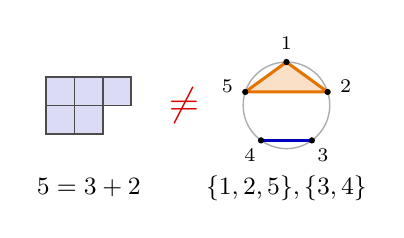
\begin{tikzpicture}
\fill[cA!14] (0,0) -- (0.36,0) -- (0.36,0.36) -- (0,0.36) -- cycle;
\draw[gray!60!black,line width=0.6pt] (0,0) -- (0.36,0) -- (0.36,0.36) -- (0,0.36) -- cycle;
\fill[cA!14] (0.36,0) -- (0.72,0) -- (0.72,0.36) -- (0.36,0.36) -- cycle;
\draw[gray!60!black,line width=0.6pt] (0.36,0) -- (0.72,0) -- (0.72,0.36) -- (0.36,0.36) -- cycle;
\fill[cA!14] (0.72,0) -- (1.08,0) -- (1.08,0.36) -- (0.72,0.36) -- cycle;
\draw[gray!60!black,line width=0.6pt] (0.72,0) -- (1.08,0) -- (1.08,0.36) -- (0.72,0.36) -- cycle;
\fill[cA!14] (0,-0.36) -- (0.36,-0.36) -- (0.36,0) -- (0,0) -- cycle;
\draw[gray!60!black,line width=0.6pt] (0,-0.36) -- (0.36,-0.36) -- (0.36,0) -- (0,0) -- cycle;
\fill[cA!14] (0.36,-0.36) -- (0.72,-0.36) -- (0.72,0) -- (0.36,0) -- cycle;
\draw[gray!60!black,line width=0.6pt] (0.36,-0.36) -- (0.72,-0.36) -- (0.72,0) -- (0.36,0) -- cycle;
\node[font=\small] at (0.54,-1.05) {$5=3+2$};
\node[font=\Large,text=cBad] at (1.75,0) {$\neq$};
\node[font=\small] at (3.05,-1.05) {$\{1,2,5\},\{3,4\}$};
\draw[gray!65,line width=0.5pt] (3.05,0) circle (0.55);
\draw[tri] (3.05,0.55) -- (3.573,0.17) -- (2.527,0.17) -- cycle;
\draw[chord] (3.373,-0.445) -- (2.727,-0.445);
\fill (3.05,0.55) circle (0.04);
\node[font=\scriptsize] at (3.05,0.79) {1};
\fill (3.573,0.17) circle (0.04);
\node[font=\scriptsize] at (3.801,0.244) {2};
\fill (3.373,-0.445) circle (0.04);
\node[font=\scriptsize] at (3.514,-0.639) {3};
\fill (2.727,-0.445) circle (0.04);
\node[font=\scriptsize] at (2.586,-0.639) {4};
\fill (2.527,0.17) circle (0.04);
\node[font=\scriptsize] at (2.299,0.244) {5};
\end{tikzpicture}}

% 附錄 A 第 3 段：A.9 堆疊與佇列排序（M09）、A.10 模式迴避（M10）、A.11 整數分割與 Young 表（M11）
% 圖由 mit/make_figs_part3.py 產生；文中的數字都在該檔的 check_numbers() 裡驗算。

% ---------------------------------------------------------------------
\subsection{堆疊與佇列排序}\label{sec:m09}

把 $1,2,\ldots,n$ 的一個排列 $w=w_1w_2\cdots w_n$ 從左到右一個一個送進一台機器，
希望它依序輸出 $1,2,\ldots,n$；機器中間只有一個暫放的容器 \mitref{L3}。哪些排列排得出來？

\textbf{堆疊（後進先出）}只能從頂端放入、拿出。規則：頂端正好是下一個要輸出的數就\textbf{彈出}，
否則把下一個輸入\textbf{推入}；輸入用完而頂端不對就失敗。每一步其實沒有選擇（頂端對時若改成推入，
新推入的數比它大，會把它永遠壓住），所以照規則做會失敗，就表示怎麼做都排不出來。
例：$4213$ 依序推入 4、2、1，彈出 1、2，推入 3，彈出 3、4，輸出 $1,2,3,4$。

\textbf{佇列＋插隊線（先進先出）}從尾端排入、從頭端出列；另有一條插隊線，讓正好輪到的數直接輸出。
佇列排序有幾種版本，本講義與動畫 M09 的規則是：佇列頭正好是下一個要輸出的數就\textbf{出列}；
否則，下一個輸入正好是它就走\textbf{插隊線}；再否則把它\textbf{排入}佇列尾；輸入用完而佇列頭不對就失敗。
這也不會錯過任何排法（佇列頭對時先出列不吃虧；佇列頭不對時，輪到的數若去排隊，就會卡在它後面）。
例：$231$ 依序排入 2、3，1 走插隊線，出列 2、3。兩種規則都由程式對 $n\le 6$ 窮舉所有走法核對過。

\begin{figure}[H]
\centering
\FigMnineStuck
\caption{卡住的那一刻。(a) 堆疊排 $231$：輸出 1 之後要輸出 \textcolor{cB}{2}，它卻被 \textcolor{cBad}{3} 壓在下面。
(b) 佇列＋插隊線排 $321$：1 走插隊線之後要輸出 \textcolor{cB}{2}，它卻排在 \textcolor{cBad}{3} 後面。}
\label{fig:m09-stuck}
\end{figure}

說 $w$ 含有 $231$，是指 $w$ 裡有三個數依序是「中、大、小」（不必相鄰）；含有 $321$ 則是「大、中、小」
（精確的定義見第~\ref{sec:m10} 節）。結果如下 \mitref{L3}：

\begin{thmbox}[可排序的排列]
\begin{enumerate}[leftmargin=1.6em]
  \item 用堆疊排得出來 $\iff$ $w$ 避開 $231$（不含 $231$）。
  \item 用佇列＋插隊線排得出來 $\iff$ $w$ 避開 $321$。
\end{enumerate}
兩種排得出來的排列都恰有 $C_n$ 個。例如 $n=3$ 的 6 個排列中，堆疊只排不出 $231$，
佇列＋插隊線只排不出 $321$，各有 $5=C_3$ 個；$n=4$ 時各有 $14=C_4$ 個。
\end{thmbox}

\begin{notebox}[為什麼]
\textbf{堆疊。}若 $b,c,a$ 依序出現且 $a<b<c$：$c$ 到的時候 $a$ 還沒來，$b$、$c$ 只能先後推入，
$c$ 壓住了必須先輸出的 $b$（圖~\ref{fig:m09-stuck}(a)）。反過來，若照規則做卡住了：要輸出的 $m$ 在堆疊裡，
緊壓在它上面的是某個 $x>m$。$x$ 推入時 $m$ 在頂端卻沒有彈出，可見那時要輸出的是更小的 $a$；
$a$ 不在 $m$ 下面（否則永遠出不來），只能還在輸入裡、在 $x$ 之後，於是 $m,x,a$ 是「中、大、小」。

\textbf{佇列。}若 $c,b,a$ 依序出現且 $c>b>a$：$c$、$b$ 到的時候 $a$ 還沒輸出，兩者都只能排隊，
$c$ 擋在必須先輸出的 $b$ 前面（圖~\ref{fig:m09-stuck}(b)）。反過來，若 $w$ 避開 $321$，
佇列由頭到尾永遠遞增：若 $x$ 排入時佇列裡已有 $y>x$，此刻要輸出的 $a<x$ 不在佇列裡
（否則它是佇列裡最小的，就在佇列頭，應該先出列），只能還在輸入裡、在 $x$ 之後，於是 $y,x,a$ 是 $321$。
佇列一直遞增，輸入用完時要輸出的數就在佇列頭，不會卡住。
\end{notebox}

\begin{keybox}[推入 $=$ U，彈出 $=$ D]
堆疊排序時，把推入記成 U、彈出記成 D。每個數恰好推入一次、彈出一次，而且彈出之前一定已經推入，
所以得到一條 Dyck 路徑，例如 $4213\mapsto$ UUUDDUDD。
反過來，從 Dyck 路徑可以讀回排列：第 $k$ 個 D 彈出的是 $k$，和它配對的 U 推入的就是同一個數。
所以堆疊排得出來的排列與 Dyck 路徑一一對應，個數是 $C_n$。
同一個數的推入與彈出連起來，正好是第~\ref{sec:m08} 節由 Dyck 路徑得到的不交叉配對；
貫穿的例子 UUDUDD 對應的排列是 $312$。佇列那一邊的個數見下一節末。
\end{keybox}

% ---------------------------------------------------------------------
\subsection{模式迴避}\label{sec:m10}

\textbf{定義} \mitref{L3}。設 $w$ 是 $1,\ldots,n$ 的排列，$\pi$ 是 $1,\ldots,k$ 的排列（$k\le n$）。
若能在 $w$ 裡挑出 $k$ 個數（保持原來的先後，不必相鄰），它們的大小順序和 $\pi$ 一樣，
就說 $w$ \textbf{含有}模式 $\pi$；否則說 $w$ \textbf{避開} $\pi$（$\pi$-avoiding）。

\textbf{例。}$w=41532$ 的第 1、3、4 個數是 $4,5,3$，大小順序是「中、大、小」，和 $231$ 一樣，
所以 $41532$ 含有 $231$。再看 $52143$：從 5 個數挑 3 個共有 $\binom{5}{3}=10$ 種挑法，
逐一檢查，得到的模式只有 $321,312,213,132$，沒有 $231$，所以 $52143$ 避開 $231$（它也能用堆疊排序）。
把排列畫成點圖（第 $i$ 個數畫在高度 $w_i$），含有 $\pi$ 就是能挑出 $k$ 個點，形狀和 $\pi$ 的點圖一樣（圖~\ref{fig:m10-plots}）。

\begin{figure}[H]
\centering
\FigMtenPlots
\caption{排列的點圖。$41532$ 的 \textcolor{cTop}{4, 5, 3} 和模式 $231$ 的形狀相同；$52143$ 挑不出這個形狀。}
\label{fig:m10-plots}
\end{figure}

\textbf{全部列出來。}$n=3$ 的 6 個排列中只有 $231$ 自己含有 $231$，5 個避開；
$n=4$ 的 24 個排列中 14 個避開（圖~\ref{fig:m10-grid}）。又是 $C_3=5$、$C_4=14$。

\begin{figure}[H]
\centering
\FigMtenGrid
\caption{$n=3$ 與 $n=4$ 的全部排列（字典序）。\textcolor{cA}{藍底}：避開 $231$；
灰字：含有 $231$，\textcolor{cBad}{紅字}是找到的第一個。}
\label{fig:m10-grid}
\end{figure}

\begin{thmbox}[定理]
堆疊可排序 $\iff$ 避開 $231$（第~\ref{sec:m09} 節）。而且對\textbf{每一個}長度 3 的模式 $\pi$，
$1,\ldots,n$ 的排列中避開 $\pi$ 的都恰有 $C_n$ 個 \mitref{L3}。
程式把 $123,132,213,231,312,321$ 逐一數出，六個模式的數字完全相同：
\begin{center}
\begin{tabular}{c|cccccc}
$n$ & 1 & 2 & 3 & 4 & 5 & 6\\
\hline
避開 $\pi$ 的個數 & 1 & 2 & 5 & 14 & 42 & 132
\end{tabular}
\end{center}
\end{thmbox}

\textbf{為什麼避開 $231$ 的有 $C_n$ 個：根＋左＋右。}看最大的數 $n$ 的位置，寫成 $w=L\,n\,R$。
若 $L$ 裡有某個數大於 $R$ 裡的某個數，這兩個數和 $n$ 就是「中、大、小」。所以
\[
\text{$w$ 避開 $231$}\iff\text{$L$ 的數全部小於 $R$ 的數，而且 $L$、$R$ 各自避開 $231$}.
\]
（反方向：$L$ 全部小於 $R$ 時，一組「中、大、小」不可能跨在 $L$、$R$ 兩邊。）
這時 $L$ 是 $1,\ldots,k$ 的排列、$R$ 是 $k+1,\ldots,n-1$ 的排列。$n$ 是\textcolor{cTop}{根}、
$L$ 是\textcolor{cLeft}{左}、$R$ 是\textcolor{cRight}{右}，個數是 $\sum_{k=0}^{n-1}C_kC_{n-1-k}$，
正是遞迴式 \eqref{eq:segner}。例：$\textcolor{cLeft}{21}\,\textcolor{cTop}{5}\,\textcolor{cRight}{34}$ 避開 $231$；
$\textcolor{cLeft}{41}\,\textcolor{cTop}{5}\,\textcolor{cRight}{32}$ 左邊的 $4$ 大於右邊的 $3$，$4,5,3$ 就是前面找到的那個 $231$。

\textbf{六個模式只有兩類。}把排列左右反轉（倒過來讀）或上下翻轉（每個數 $x$ 換成 $n+1-x$），
含有的模式也跟著反轉或翻轉：$231$ 反轉成 $132$、翻轉成 $213$、兩個都做成 $312$，所以這四個模式的個數相同。
$123$ 與 $321$ 互為反轉，是另一類；它們也是 $C_n$ 個（$321$ 就是第~\ref{sec:m09} 節的佇列＋插隊線），
但需要另一種一一對應，這裡不證明。

% ---------------------------------------------------------------------
\subsection{整數分割與 Young 表}\label{sec:m11}

L3 最後換到另一種「分割」\mitref{L3}。$n$ 的一個\textbf{整數分割}是把 $n$ 寫成由大到小排好的正整數之和：
$\lambda=(\lambda_1,\ldots,\lambda_k)$，$\lambda_1\ge\lambda_2\ge\cdots\ge\lambda_k>0$，$\lambda_1+\cdots+\lambda_k=n$，
記作 $\lambda\vdash n$。$5$ 的整數分割有 7 個：
$5,\ 4+1,\ 3+2,\ 3+1+1,\ 2+2+1,\ 2+1+1+1,\ 1+1+1+1+1$。
如果順序不同算不同的，叫做\textbf{合成}（composition）：$5$ 的合成有 $2^4=16$ 個
（5 個 1 排成一列，中間 4 個空隙各自決定切或不切），其中由大到小排好的 7 個正是 5 的整數分割。
所以 $3+2$ 是整數分割 $(3,2)$；$2+3$ 不是由大到小，只是合成 $(2,3)$。

\begin{notebox}[注意：兩種「分割」不是同一個東西]
\begin{minipage}[c]{0.67\linewidth}
這裡的\textbf{整數分割}只看每一份有多大。Chu 論文的分割（第 2 節）是\textbf{集合分割}：
把圓周上\textbf{有編號的點}分成區塊，例如 $\{1,2,5\},\{3,4\}$（圖~\ref{fig:paper} 的第 5 個）。
兩者只有一點關係：把集合分割的區塊大小由大到小排好，就得到一個整數分割。
Chu 的 $\vn$、$\vv$ 指定的正是這個整數分割，例如第 3 節原文例子 $\vn=(1,1)$、$\vv=(2,3)$
指定區塊大小 $3$ 與 $2$，也就是 $(3,2)\vdash 5$；但 Chu 數的是不交叉的集合分割本身（這個例子有 5 個）。
L1--4 也沒有發展一般的不交叉集合分割 \mitref{L1--4}。
\end{minipage}\hfill
\begin{minipage}[c]{0.31\linewidth}
\centering
\FigMelevenWarn
\end{minipage}
\end{notebox}

\textbf{Young 圖} \mitref{L3}。把 $\lambda$ 畫成第 $i$ 列有 $\lambda_i$ 個格子、每列靠左、
由上往下不變長的圖（英式畫法）。圖~\ref{fig:m11-young} 上排左邊是 $\lambda=(5,3,3,2,1)\vdash 14$，
右邊是 5 的 7 個整數分割。

\textbf{標準 Young 表（SYT）} \mitref{L3}。把 $1,2,\ldots,n$ 各填一次到形狀 $\lambda$ 的格子裡，
使\textbf{每一列由左到右遞增、每一行由上到下遞增}。形狀 $\lambda$ 的 SYT 個數記作 $f^\lambda$。
例如圖~\ref{fig:m11-young} 下排最左邊的表（第一列 $1,2,4$、第二列 $3,5$）是 SYT，它就是貫穿例子的 SYT 拿掉 6；
旁邊的表每一列都遞增，但第 2 行上面是 4、下面是 3，不是 SYT。
形狀 $(3,2)$ 的 SYT 全部列出來恰有 5 個：$f^{(3,2)}=5$。

\begin{figure}[H]
\centering
\FigMelevenYoungSYT
\caption{上排：$\lambda=(5,3,3,2,1)$ 的 Young 圖，共 14 格（小字是每列的長度）；右邊是 5 的 7 個整數分割。
下排：一個 SYT 與一個反例（\textcolor{cBad}{紅格}所在的第 2 行不遞增）；右邊是形狀 $(3,2)$ 的全部 5 個 SYT，
第 2 個（深色）就是最左邊那一個。}
\label{fig:m11-young}
\end{figure}

L4 的問題就是：$f^\lambda$ 怎麼算？第~\ref{sec:m12} 節會看到 $f^{(n,n)}=C_n$（例如 $f^{(3,3)}=C_3=5$），
第~\ref{sec:m13} 節的鉤長公式則給出一般的 $f^\lambda$。

% 附錄 A 第 4 段：A.12–A.14（動畫 M12–M14，MIT 18.212 L4）
% 圖由 mit/make_figs_part4.py 產生（含數字檢查）；格子 (i,j) = 第 i 列第 j 行，1 起算。
% figs_part4.tex —— 由 mit/make_figs_part4.py 產生，請勿手動修改。
% 重新產生：python mit/make_figs_part4.py（附錄 A.12–A.14，動畫 M12–M14）

\newcommand{\FigMXIIConvert}{%
\begin{tikzpicture}
\fill[cLeft!20] (0,0) -- (0.62,0) -- (0.62,-0.62) -- (0,-0.62) -- cycle;
\fill[cLeft!20] (0.62,0) -- (1.24,0) -- (1.24,-0.62) -- (0.62,-0.62) -- cycle;
\fill[cLeft!20] (1.24,0) -- (1.86,0) -- (1.86,-0.62) -- (1.24,-0.62) -- cycle;
\fill[cRight!18] (0,-0.62) -- (0.62,-0.62) -- (0.62,-1.24) -- (0,-1.24) -- cycle;
\fill[cRight!18] (0.62,-0.62) -- (1.24,-0.62) -- (1.24,-1.24) -- (0.62,-1.24) -- cycle;
\fill[cRight!18] (1.24,-0.62) -- (1.86,-0.62) -- (1.86,-1.24) -- (1.24,-1.24) -- cycle;
\draw[gray!70!black,line width=0.5pt] (0,0) -- (0.62,0) -- (0.62,-0.62) -- (0,-0.62) -- cycle;
\draw[gray!70!black,line width=0.5pt] (0.62,0) -- (1.24,0) -- (1.24,-0.62) -- (0.62,-0.62) -- cycle;
\draw[gray!70!black,line width=0.5pt] (1.24,0) -- (1.86,0) -- (1.86,-0.62) -- (1.24,-0.62) -- cycle;
\draw[gray!70!black,line width=0.5pt] (0,-0.62) -- (0.62,-0.62) -- (0.62,-1.24) -- (0,-1.24) -- cycle;
\draw[gray!70!black,line width=0.5pt] (0.62,-0.62) -- (1.24,-0.62) -- (1.24,-1.24) -- (0.62,-1.24) -- cycle;
\draw[gray!70!black,line width=0.5pt] (1.24,-0.62) -- (1.86,-0.62) -- (1.86,-1.24) -- (1.24,-1.24) -- cycle;
\node[font=\small,inner sep=0pt] at (0.31,-0.31) {$1$};
\node[font=\small,inner sep=0pt] at (0.93,-0.31) {$2$};
\node[font=\small,inner sep=0pt] at (1.55,-0.31) {$4$};
\node[font=\small,inner sep=0pt] at (0.31,-0.93) {$3$};
\node[font=\small,inner sep=0pt] at (0.93,-0.93) {$5$};
\node[font=\small,inner sep=0pt] at (1.55,-0.93) {$6$};
\node[anchor=west,font=\small,text=cLeft] at (1.98,-0.31) {$\to\mathrm{U}$};
\node[anchor=west,font=\small,text=cRight] at (1.98,-0.93) {$\to\mathrm{D}$};
\draw[-{Stealth[length=5pt]},gray!60!black,line width=0.7pt] (3.1,-0.62) -- (4,-0.62);
\draw[gray!55,line width=0.4pt] (4.35,-0.9) -- (7.11,-0.9);
\draw[cLeft,line width=1.5pt,line cap=round] (4.35,-0.9) -- (4.81,-0.44);
\draw[cLeft,line width=1.5pt,line cap=round] (4.81,-0.44) -- (5.27,0.02);
\draw[cRight,line width=1.5pt,line cap=round] (5.27,0.02) -- (5.73,-0.44);
\draw[cLeft,line width=1.5pt,line cap=round] (5.73,-0.44) -- (6.19,0.02);
\draw[cRight,line width=1.5pt,line cap=round] (6.19,0.02) -- (6.65,-0.44);
\draw[cRight,line width=1.5pt,line cap=round] (6.65,-0.44) -- (7.11,-0.9);
\fill[black] (4.35,-0.9) circle (0.035);
\fill[black] (4.81,-0.44) circle (0.035);
\fill[black] (5.27,0.02) circle (0.035);
\fill[black] (5.73,-0.44) circle (0.035);
\fill[black] (6.19,0.02) circle (0.035);
\fill[black] (6.65,-0.44) circle (0.035);
\fill[black] (7.11,-0.9) circle (0.035);
\node[font=\scriptsize,text=gray!70!black] at (4.58,-1.14) {1};
\node[font=\small,text=cLeft] at (4.58,-1.46) {$\mathrm{U}$};
\node[font=\scriptsize,text=gray!70!black] at (5.04,-1.14) {2};
\node[font=\small,text=cLeft] at (5.04,-1.46) {$\mathrm{U}$};
\node[font=\scriptsize,text=gray!70!black] at (5.5,-1.14) {3};
\node[font=\small,text=cRight] at (5.5,-1.46) {$\mathrm{D}$};
\node[font=\scriptsize,text=gray!70!black] at (5.96,-1.14) {4};
\node[font=\small,text=cLeft] at (5.96,-1.46) {$\mathrm{U}$};
\node[font=\scriptsize,text=gray!70!black] at (6.42,-1.14) {5};
\node[font=\small,text=cRight] at (6.42,-1.46) {$\mathrm{D}$};
\node[font=\scriptsize,text=gray!70!black] at (6.88,-1.14) {6};
\node[font=\small,text=cRight] at (6.88,-1.46) {$\mathrm{D}$};
\node[anchor=east,font=\scriptsize,text=gray!70!black] at (4.05,-1.14) {步};
\end{tikzpicture}}

\newcommand{\FigMXIIAll}{%
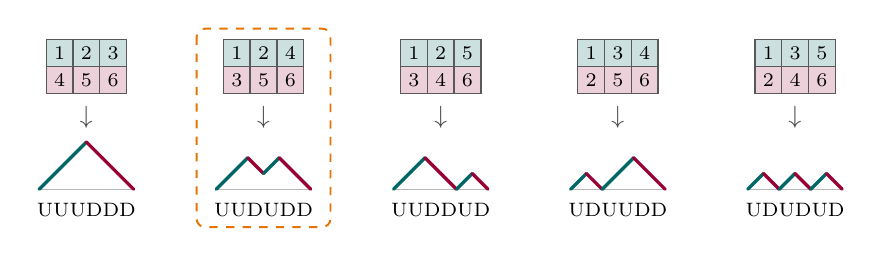
\begin{tikzpicture}
\fill[cLeft!20] (-0.51,0) -- (-0.17,0) -- (-0.17,-0.34) -- (-0.51,-0.34) -- cycle;
\fill[cLeft!20] (-0.17,0) -- (0.17,0) -- (0.17,-0.34) -- (-0.17,-0.34) -- cycle;
\fill[cLeft!20] (0.17,0) -- (0.51,0) -- (0.51,-0.34) -- (0.17,-0.34) -- cycle;
\fill[cRight!18] (-0.51,-0.34) -- (-0.17,-0.34) -- (-0.17,-0.68) -- (-0.51,-0.68) -- cycle;
\fill[cRight!18] (-0.17,-0.34) -- (0.17,-0.34) -- (0.17,-0.68) -- (-0.17,-0.68) -- cycle;
\fill[cRight!18] (0.17,-0.34) -- (0.51,-0.34) -- (0.51,-0.68) -- (0.17,-0.68) -- cycle;
\draw[gray!70!black,line width=0.5pt] (-0.51,0) -- (-0.17,0) -- (-0.17,-0.34) -- (-0.51,-0.34) -- cycle;
\draw[gray!70!black,line width=0.5pt] (-0.17,0) -- (0.17,0) -- (0.17,-0.34) -- (-0.17,-0.34) -- cycle;
\draw[gray!70!black,line width=0.5pt] (0.17,0) -- (0.51,0) -- (0.51,-0.34) -- (0.17,-0.34) -- cycle;
\draw[gray!70!black,line width=0.5pt] (-0.51,-0.34) -- (-0.17,-0.34) -- (-0.17,-0.68) -- (-0.51,-0.68) -- cycle;
\draw[gray!70!black,line width=0.5pt] (-0.17,-0.34) -- (0.17,-0.34) -- (0.17,-0.68) -- (-0.17,-0.68) -- cycle;
\draw[gray!70!black,line width=0.5pt] (0.17,-0.34) -- (0.51,-0.34) -- (0.51,-0.68) -- (0.17,-0.68) -- cycle;
\node[font=\scriptsize,inner sep=0pt] at (-0.34,-0.17) {$1$};
\node[font=\scriptsize,inner sep=0pt] at (0,-0.17) {$2$};
\node[font=\scriptsize,inner sep=0pt] at (0.34,-0.17) {$3$};
\node[font=\scriptsize,inner sep=0pt] at (-0.34,-0.51) {$4$};
\node[font=\scriptsize,inner sep=0pt] at (0,-0.51) {$5$};
\node[font=\scriptsize,inner sep=0pt] at (0.34,-0.51) {$6$};
\node[font=\small,text=gray!60!black] at (0,-0.98) {$\downarrow$};
\draw[gray!55,line width=0.4pt] (-0.6,-1.9) -- (0.6,-1.9);
\draw[cLeft,line width=1.2pt,line cap=round] (-0.6,-1.9) -- (-0.4,-1.7);
\draw[cLeft,line width=1.2pt,line cap=round] (-0.4,-1.7) -- (-0.2,-1.5);
\draw[cLeft,line width=1.2pt,line cap=round] (-0.2,-1.5) -- (0,-1.3);
\draw[cRight,line width=1.2pt,line cap=round] (0,-1.3) -- (0.2,-1.5);
\draw[cRight,line width=1.2pt,line cap=round] (0.2,-1.5) -- (0.4,-1.7);
\draw[cRight,line width=1.2pt,line cap=round] (0.4,-1.7) -- (0.6,-1.9);
\node[font=\scriptsize] at (0,-2.16) {$\mathrm{UUUDDD}$};
\fill[cLeft!20] (1.74,0) -- (2.08,0) -- (2.08,-0.34) -- (1.74,-0.34) -- cycle;
\fill[cLeft!20] (2.08,0) -- (2.42,0) -- (2.42,-0.34) -- (2.08,-0.34) -- cycle;
\fill[cLeft!20] (2.42,0) -- (2.76,0) -- (2.76,-0.34) -- (2.42,-0.34) -- cycle;
\fill[cRight!18] (1.74,-0.34) -- (2.08,-0.34) -- (2.08,-0.68) -- (1.74,-0.68) -- cycle;
\fill[cRight!18] (2.08,-0.34) -- (2.42,-0.34) -- (2.42,-0.68) -- (2.08,-0.68) -- cycle;
\fill[cRight!18] (2.42,-0.34) -- (2.76,-0.34) -- (2.76,-0.68) -- (2.42,-0.68) -- cycle;
\draw[gray!70!black,line width=0.5pt] (1.74,0) -- (2.08,0) -- (2.08,-0.34) -- (1.74,-0.34) -- cycle;
\draw[gray!70!black,line width=0.5pt] (2.08,0) -- (2.42,0) -- (2.42,-0.34) -- (2.08,-0.34) -- cycle;
\draw[gray!70!black,line width=0.5pt] (2.42,0) -- (2.76,0) -- (2.76,-0.34) -- (2.42,-0.34) -- cycle;
\draw[gray!70!black,line width=0.5pt] (1.74,-0.34) -- (2.08,-0.34) -- (2.08,-0.68) -- (1.74,-0.68) -- cycle;
\draw[gray!70!black,line width=0.5pt] (2.08,-0.34) -- (2.42,-0.34) -- (2.42,-0.68) -- (2.08,-0.68) -- cycle;
\draw[gray!70!black,line width=0.5pt] (2.42,-0.34) -- (2.76,-0.34) -- (2.76,-0.68) -- (2.42,-0.68) -- cycle;
\node[font=\scriptsize,inner sep=0pt] at (1.91,-0.17) {$1$};
\node[font=\scriptsize,inner sep=0pt] at (2.25,-0.17) {$2$};
\node[font=\scriptsize,inner sep=0pt] at (2.59,-0.17) {$4$};
\node[font=\scriptsize,inner sep=0pt] at (1.91,-0.51) {$3$};
\node[font=\scriptsize,inner sep=0pt] at (2.25,-0.51) {$5$};
\node[font=\scriptsize,inner sep=0pt] at (2.59,-0.51) {$6$};
\node[font=\small,text=gray!60!black] at (2.25,-0.98) {$\downarrow$};
\draw[gray!55,line width=0.4pt] (1.65,-1.9) -- (2.85,-1.9);
\draw[cLeft,line width=1.2pt,line cap=round] (1.65,-1.9) -- (1.85,-1.7);
\draw[cLeft,line width=1.2pt,line cap=round] (1.85,-1.7) -- (2.05,-1.5);
\draw[cRight,line width=1.2pt,line cap=round] (2.05,-1.5) -- (2.25,-1.7);
\draw[cLeft,line width=1.2pt,line cap=round] (2.25,-1.7) -- (2.45,-1.5);
\draw[cRight,line width=1.2pt,line cap=round] (2.45,-1.5) -- (2.65,-1.7);
\draw[cRight,line width=1.2pt,line cap=round] (2.65,-1.7) -- (2.85,-1.9);
\node[font=\scriptsize] at (2.25,-2.16) {$\mathrm{UUDUDD}$};
\draw[cTop,dashed,line width=0.7pt,rounded corners=3pt] (1.4,0.14) rectangle (3.1,-2.38);
\fill[cLeft!20] (3.99,0) -- (4.33,0) -- (4.33,-0.34) -- (3.99,-0.34) -- cycle;
\fill[cLeft!20] (4.33,0) -- (4.67,0) -- (4.67,-0.34) -- (4.33,-0.34) -- cycle;
\fill[cLeft!20] (4.67,0) -- (5.01,0) -- (5.01,-0.34) -- (4.67,-0.34) -- cycle;
\fill[cRight!18] (3.99,-0.34) -- (4.33,-0.34) -- (4.33,-0.68) -- (3.99,-0.68) -- cycle;
\fill[cRight!18] (4.33,-0.34) -- (4.67,-0.34) -- (4.67,-0.68) -- (4.33,-0.68) -- cycle;
\fill[cRight!18] (4.67,-0.34) -- (5.01,-0.34) -- (5.01,-0.68) -- (4.67,-0.68) -- cycle;
\draw[gray!70!black,line width=0.5pt] (3.99,0) -- (4.33,0) -- (4.33,-0.34) -- (3.99,-0.34) -- cycle;
\draw[gray!70!black,line width=0.5pt] (4.33,0) -- (4.67,0) -- (4.67,-0.34) -- (4.33,-0.34) -- cycle;
\draw[gray!70!black,line width=0.5pt] (4.67,0) -- (5.01,0) -- (5.01,-0.34) -- (4.67,-0.34) -- cycle;
\draw[gray!70!black,line width=0.5pt] (3.99,-0.34) -- (4.33,-0.34) -- (4.33,-0.68) -- (3.99,-0.68) -- cycle;
\draw[gray!70!black,line width=0.5pt] (4.33,-0.34) -- (4.67,-0.34) -- (4.67,-0.68) -- (4.33,-0.68) -- cycle;
\draw[gray!70!black,line width=0.5pt] (4.67,-0.34) -- (5.01,-0.34) -- (5.01,-0.68) -- (4.67,-0.68) -- cycle;
\node[font=\scriptsize,inner sep=0pt] at (4.16,-0.17) {$1$};
\node[font=\scriptsize,inner sep=0pt] at (4.5,-0.17) {$2$};
\node[font=\scriptsize,inner sep=0pt] at (4.84,-0.17) {$5$};
\node[font=\scriptsize,inner sep=0pt] at (4.16,-0.51) {$3$};
\node[font=\scriptsize,inner sep=0pt] at (4.5,-0.51) {$4$};
\node[font=\scriptsize,inner sep=0pt] at (4.84,-0.51) {$6$};
\node[font=\small,text=gray!60!black] at (4.5,-0.98) {$\downarrow$};
\draw[gray!55,line width=0.4pt] (3.9,-1.9) -- (5.1,-1.9);
\draw[cLeft,line width=1.2pt,line cap=round] (3.9,-1.9) -- (4.1,-1.7);
\draw[cLeft,line width=1.2pt,line cap=round] (4.1,-1.7) -- (4.3,-1.5);
\draw[cRight,line width=1.2pt,line cap=round] (4.3,-1.5) -- (4.5,-1.7);
\draw[cRight,line width=1.2pt,line cap=round] (4.5,-1.7) -- (4.7,-1.9);
\draw[cLeft,line width=1.2pt,line cap=round] (4.7,-1.9) -- (4.9,-1.7);
\draw[cRight,line width=1.2pt,line cap=round] (4.9,-1.7) -- (5.1,-1.9);
\node[font=\scriptsize] at (4.5,-2.16) {$\mathrm{UUDDUD}$};
\fill[cLeft!20] (6.24,0) -- (6.58,0) -- (6.58,-0.34) -- (6.24,-0.34) -- cycle;
\fill[cLeft!20] (6.58,0) -- (6.92,0) -- (6.92,-0.34) -- (6.58,-0.34) -- cycle;
\fill[cLeft!20] (6.92,0) -- (7.26,0) -- (7.26,-0.34) -- (6.92,-0.34) -- cycle;
\fill[cRight!18] (6.24,-0.34) -- (6.58,-0.34) -- (6.58,-0.68) -- (6.24,-0.68) -- cycle;
\fill[cRight!18] (6.58,-0.34) -- (6.92,-0.34) -- (6.92,-0.68) -- (6.58,-0.68) -- cycle;
\fill[cRight!18] (6.92,-0.34) -- (7.26,-0.34) -- (7.26,-0.68) -- (6.92,-0.68) -- cycle;
\draw[gray!70!black,line width=0.5pt] (6.24,0) -- (6.58,0) -- (6.58,-0.34) -- (6.24,-0.34) -- cycle;
\draw[gray!70!black,line width=0.5pt] (6.58,0) -- (6.92,0) -- (6.92,-0.34) -- (6.58,-0.34) -- cycle;
\draw[gray!70!black,line width=0.5pt] (6.92,0) -- (7.26,0) -- (7.26,-0.34) -- (6.92,-0.34) -- cycle;
\draw[gray!70!black,line width=0.5pt] (6.24,-0.34) -- (6.58,-0.34) -- (6.58,-0.68) -- (6.24,-0.68) -- cycle;
\draw[gray!70!black,line width=0.5pt] (6.58,-0.34) -- (6.92,-0.34) -- (6.92,-0.68) -- (6.58,-0.68) -- cycle;
\draw[gray!70!black,line width=0.5pt] (6.92,-0.34) -- (7.26,-0.34) -- (7.26,-0.68) -- (6.92,-0.68) -- cycle;
\node[font=\scriptsize,inner sep=0pt] at (6.41,-0.17) {$1$};
\node[font=\scriptsize,inner sep=0pt] at (6.75,-0.17) {$3$};
\node[font=\scriptsize,inner sep=0pt] at (7.09,-0.17) {$4$};
\node[font=\scriptsize,inner sep=0pt] at (6.41,-0.51) {$2$};
\node[font=\scriptsize,inner sep=0pt] at (6.75,-0.51) {$5$};
\node[font=\scriptsize,inner sep=0pt] at (7.09,-0.51) {$6$};
\node[font=\small,text=gray!60!black] at (6.75,-0.98) {$\downarrow$};
\draw[gray!55,line width=0.4pt] (6.15,-1.9) -- (7.35,-1.9);
\draw[cLeft,line width=1.2pt,line cap=round] (6.15,-1.9) -- (6.35,-1.7);
\draw[cRight,line width=1.2pt,line cap=round] (6.35,-1.7) -- (6.55,-1.9);
\draw[cLeft,line width=1.2pt,line cap=round] (6.55,-1.9) -- (6.75,-1.7);
\draw[cLeft,line width=1.2pt,line cap=round] (6.75,-1.7) -- (6.95,-1.5);
\draw[cRight,line width=1.2pt,line cap=round] (6.95,-1.5) -- (7.15,-1.7);
\draw[cRight,line width=1.2pt,line cap=round] (7.15,-1.7) -- (7.35,-1.9);
\node[font=\scriptsize] at (6.75,-2.16) {$\mathrm{UDUUDD}$};
\fill[cLeft!20] (8.49,0) -- (8.83,0) -- (8.83,-0.34) -- (8.49,-0.34) -- cycle;
\fill[cLeft!20] (8.83,0) -- (9.17,0) -- (9.17,-0.34) -- (8.83,-0.34) -- cycle;
\fill[cLeft!20] (9.17,0) -- (9.51,0) -- (9.51,-0.34) -- (9.17,-0.34) -- cycle;
\fill[cRight!18] (8.49,-0.34) -- (8.83,-0.34) -- (8.83,-0.68) -- (8.49,-0.68) -- cycle;
\fill[cRight!18] (8.83,-0.34) -- (9.17,-0.34) -- (9.17,-0.68) -- (8.83,-0.68) -- cycle;
\fill[cRight!18] (9.17,-0.34) -- (9.51,-0.34) -- (9.51,-0.68) -- (9.17,-0.68) -- cycle;
\draw[gray!70!black,line width=0.5pt] (8.49,0) -- (8.83,0) -- (8.83,-0.34) -- (8.49,-0.34) -- cycle;
\draw[gray!70!black,line width=0.5pt] (8.83,0) -- (9.17,0) -- (9.17,-0.34) -- (8.83,-0.34) -- cycle;
\draw[gray!70!black,line width=0.5pt] (9.17,0) -- (9.51,0) -- (9.51,-0.34) -- (9.17,-0.34) -- cycle;
\draw[gray!70!black,line width=0.5pt] (8.49,-0.34) -- (8.83,-0.34) -- (8.83,-0.68) -- (8.49,-0.68) -- cycle;
\draw[gray!70!black,line width=0.5pt] (8.83,-0.34) -- (9.17,-0.34) -- (9.17,-0.68) -- (8.83,-0.68) -- cycle;
\draw[gray!70!black,line width=0.5pt] (9.17,-0.34) -- (9.51,-0.34) -- (9.51,-0.68) -- (9.17,-0.68) -- cycle;
\node[font=\scriptsize,inner sep=0pt] at (8.66,-0.17) {$1$};
\node[font=\scriptsize,inner sep=0pt] at (9,-0.17) {$3$};
\node[font=\scriptsize,inner sep=0pt] at (9.34,-0.17) {$5$};
\node[font=\scriptsize,inner sep=0pt] at (8.66,-0.51) {$2$};
\node[font=\scriptsize,inner sep=0pt] at (9,-0.51) {$4$};
\node[font=\scriptsize,inner sep=0pt] at (9.34,-0.51) {$6$};
\node[font=\small,text=gray!60!black] at (9,-0.98) {$\downarrow$};
\draw[gray!55,line width=0.4pt] (8.4,-1.9) -- (9.6,-1.9);
\draw[cLeft,line width=1.2pt,line cap=round] (8.4,-1.9) -- (8.6,-1.7);
\draw[cRight,line width=1.2pt,line cap=round] (8.6,-1.7) -- (8.8,-1.9);
\draw[cLeft,line width=1.2pt,line cap=round] (8.8,-1.9) -- (9,-1.7);
\draw[cRight,line width=1.2pt,line cap=round] (9,-1.7) -- (9.2,-1.9);
\draw[cLeft,line width=1.2pt,line cap=round] (9.2,-1.9) -- (9.4,-1.7);
\draw[cRight,line width=1.2pt,line cap=round] (9.4,-1.7) -- (9.6,-1.9);
\node[font=\scriptsize] at (9,-2.16) {$\mathrm{UDUDUD}$};
\end{tikzpicture}}

\newcommand{\FigMXIIGenGood}{%
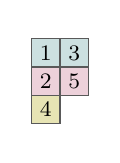
\begin{tikzpicture}[baseline={(0,-0.63)}]
\fill[cLeft!20] (0,0) -- (0.36,0) -- (0.36,-0.36) -- (0,-0.36) -- cycle;
\fill[cLeft!20] (0.36,0) -- (0.72,0) -- (0.72,-0.36) -- (0.36,-0.36) -- cycle;
\fill[cRight!18] (0,-0.36) -- (0.36,-0.36) -- (0.36,-0.72) -- (0,-0.72) -- cycle;
\fill[cRight!18] (0.36,-0.36) -- (0.72,-0.36) -- (0.72,-0.72) -- (0.36,-0.72) -- cycle;
\fill[olive!22] (0,-0.72) -- (0.36,-0.72) -- (0.36,-1.08) -- (0,-1.08) -- cycle;
\draw[gray!70!black,line width=0.5pt] (0,0) -- (0.36,0) -- (0.36,-0.36) -- (0,-0.36) -- cycle;
\draw[gray!70!black,line width=0.5pt] (0.36,0) -- (0.72,0) -- (0.72,-0.36) -- (0.36,-0.36) -- cycle;
\draw[gray!70!black,line width=0.5pt] (0,-0.36) -- (0.36,-0.36) -- (0.36,-0.72) -- (0,-0.72) -- cycle;
\draw[gray!70!black,line width=0.5pt] (0.36,-0.36) -- (0.72,-0.36) -- (0.72,-0.72) -- (0.36,-0.72) -- cycle;
\draw[gray!70!black,line width=0.5pt] (0,-0.72) -- (0.36,-0.72) -- (0.36,-1.08) -- (0,-1.08) -- cycle;
\node[font=\footnotesize,inner sep=0pt] at (0.18,-0.18) {$1$};
\node[font=\footnotesize,inner sep=0pt] at (0.54,-0.18) {$3$};
\node[font=\footnotesize,inner sep=0pt] at (0.18,-0.54) {$2$};
\node[font=\footnotesize,inner sep=0pt] at (0.54,-0.54) {$5$};
\node[font=\footnotesize,inner sep=0pt] at (0.18,-0.9) {$4$};
\path (-0.05,0.14) rectangle (0.77,-1.22);
\end{tikzpicture}}

\newcommand{\FigMXIIGenBad}{%
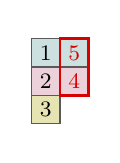
\begin{tikzpicture}[baseline={(0,-0.63)}]
\fill[cLeft!20] (0,0) -- (0.36,0) -- (0.36,-0.36) -- (0,-0.36) -- cycle;
\fill[cLeft!20] (0.36,0) -- (0.72,0) -- (0.72,-0.36) -- (0.36,-0.36) -- cycle;
\fill[cRight!18] (0,-0.36) -- (0.36,-0.36) -- (0.36,-0.72) -- (0,-0.72) -- cycle;
\fill[cRight!18] (0.36,-0.36) -- (0.72,-0.36) -- (0.72,-0.72) -- (0.36,-0.72) -- cycle;
\fill[olive!22] (0,-0.72) -- (0.36,-0.72) -- (0.36,-1.08) -- (0,-1.08) -- cycle;
\draw[gray!70!black,line width=0.5pt] (0,0) -- (0.36,0) -- (0.36,-0.36) -- (0,-0.36) -- cycle;
\draw[gray!70!black,line width=0.5pt] (0.36,0) -- (0.72,0) -- (0.72,-0.36) -- (0.36,-0.36) -- cycle;
\draw[gray!70!black,line width=0.5pt] (0,-0.36) -- (0.36,-0.36) -- (0.36,-0.72) -- (0,-0.72) -- cycle;
\draw[gray!70!black,line width=0.5pt] (0.36,-0.36) -- (0.72,-0.36) -- (0.72,-0.72) -- (0.36,-0.72) -- cycle;
\draw[gray!70!black,line width=0.5pt] (0,-0.72) -- (0.36,-0.72) -- (0.36,-1.08) -- (0,-1.08) -- cycle;
\node[font=\footnotesize,inner sep=0pt] at (0.18,-0.18) {$1$};
\node[font=\footnotesize,inner sep=0pt,text=cBad] at (0.54,-0.18) {$5$};
\node[font=\footnotesize,inner sep=0pt] at (0.18,-0.54) {$2$};
\node[font=\footnotesize,inner sep=0pt,text=cBad] at (0.54,-0.54) {$4$};
\node[font=\footnotesize,inner sep=0pt] at (0.18,-0.9) {$3$};
\draw[cBad,line width=1pt] (0.36,0) rectangle (0.72,-0.72);
\path (-0.05,0.14) rectangle (0.77,-1.22);
\end{tikzpicture}}

\newcommand{\FigMXIIIHook}{%
\begin{tikzpicture}
\fill[yellow!55] (1.24,0) -- (1.86,0) -- (1.86,-0.62) -- (1.24,-0.62) -- cycle;
\fill[yellow!55] (1.86,0) -- (2.48,0) -- (2.48,-0.62) -- (1.86,-0.62) -- cycle;
\fill[yellow!55] (0.62,-0.62) -- (1.24,-0.62) -- (1.24,-1.24) -- (0.62,-1.24) -- cycle;
\fill[cTop!45] (0.62,0) -- (1.24,0) -- (1.24,-0.62) -- (0.62,-0.62) -- cycle;
\draw[gray!70!black,line width=0.5pt] (0,0) -- (0.62,0) -- (0.62,-0.62) -- (0,-0.62) -- cycle;
\draw[gray!70!black,line width=0.5pt] (0.62,0) -- (1.24,0) -- (1.24,-0.62) -- (0.62,-0.62) -- cycle;
\draw[gray!70!black,line width=0.5pt] (1.24,0) -- (1.86,0) -- (1.86,-0.62) -- (1.24,-0.62) -- cycle;
\draw[gray!70!black,line width=0.5pt] (1.86,0) -- (2.48,0) -- (2.48,-0.62) -- (1.86,-0.62) -- cycle;
\draw[gray!70!black,line width=0.5pt] (0,-0.62) -- (0.62,-0.62) -- (0.62,-1.24) -- (0,-1.24) -- cycle;
\draw[gray!70!black,line width=0.5pt] (0.62,-0.62) -- (1.24,-0.62) -- (1.24,-1.24) -- (0.62,-1.24) -- cycle;
\draw[gray!70!black,line width=0.5pt] (1.24,-0.62) -- (1.86,-0.62) -- (1.86,-1.24) -- (1.24,-1.24) -- cycle;
\draw[gray!70!black,line width=0.5pt] (0,-1.24) -- (0.62,-1.24) -- (0.62,-1.86) -- (0,-1.86) -- cycle;
\node[font=\small] at (0.93,-0.31) {$c$};
\draw[orange!70!black,line width=0.6pt] (1.3,0.1) -- (1.3,0.2) -- (2.42,0.2) -- (2.42,0.1);
\node[font=\footnotesize,text=orange!70!black] at (1.86,0.43) {臂};
\draw[orange!70!black,line width=0.6pt] (0.68,-1.34) -- (0.68,-1.44) -- (1.18,-1.44) -- (1.18,-1.34);
\node[font=\footnotesize,text=orange!70!black] at (0.93,-1.67) {腿};
\node[font=\small] at (1.24,-2.41) {$h(c)=2+1+1=4$};
\draw[gray!70!black,line width=0.5pt] (4.18,0) -- (4.8,0) -- (4.8,-0.62) -- (4.18,-0.62) -- cycle;
\draw[gray!70!black,line width=0.5pt] (4.8,0) -- (5.42,0) -- (5.42,-0.62) -- (4.8,-0.62) -- cycle;
\draw[gray!70!black,line width=0.5pt] (5.42,0) -- (6.04,0) -- (6.04,-0.62) -- (5.42,-0.62) -- cycle;
\draw[gray!70!black,line width=0.5pt] (6.04,0) -- (6.66,0) -- (6.66,-0.62) -- (6.04,-0.62) -- cycle;
\draw[gray!70!black,line width=0.5pt] (4.18,-0.62) -- (4.8,-0.62) -- (4.8,-1.24) -- (4.18,-1.24) -- cycle;
\draw[gray!70!black,line width=0.5pt] (4.8,-0.62) -- (5.42,-0.62) -- (5.42,-1.24) -- (4.8,-1.24) -- cycle;
\draw[gray!70!black,line width=0.5pt] (5.42,-0.62) -- (6.04,-0.62) -- (6.04,-1.24) -- (5.42,-1.24) -- cycle;
\draw[gray!70!black,line width=0.5pt] (4.18,-1.24) -- (4.8,-1.24) -- (4.8,-1.86) -- (4.18,-1.86) -- cycle;
\node[font=\small,inner sep=0pt] at (4.49,-0.31) {$6$};
\node[font=\small,inner sep=0pt] at (5.11,-0.31) {$4$};
\node[font=\small,inner sep=0pt] at (5.73,-0.31) {$3$};
\node[font=\small,inner sep=0pt] at (6.35,-0.31) {$1$};
\node[font=\small,inner sep=0pt] at (4.49,-0.93) {$4$};
\node[font=\small,inner sep=0pt] at (5.11,-0.93) {$2$};
\node[font=\small,inner sep=0pt] at (5.73,-0.93) {$1$};
\node[font=\small,inner sep=0pt] at (4.49,-1.55) {$1$};
\node[font=\small] at (5.42,-2.41) {$H(\lambda)=576$};
\end{tikzpicture}}

\newcommand{\FigMXIIIHookSmall}{%
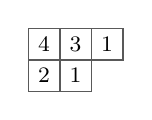
\begin{tikzpicture}[baseline={(0,-0.48)}]
\draw[gray!70!black,line width=0.5pt] (0,0) -- (0.4,0) -- (0.4,-0.4) -- (0,-0.4) -- cycle;
\draw[gray!70!black,line width=0.5pt] (0.4,0) -- (0.8,0) -- (0.8,-0.4) -- (0.4,-0.4) -- cycle;
\draw[gray!70!black,line width=0.5pt] (0.8,0) -- (1.2,0) -- (1.2,-0.4) -- (0.8,-0.4) -- cycle;
\draw[gray!70!black,line width=0.5pt] (0,-0.4) -- (0.4,-0.4) -- (0.4,-0.8) -- (0,-0.8) -- cycle;
\draw[gray!70!black,line width=0.5pt] (0.4,-0.4) -- (0.8,-0.4) -- (0.8,-0.8) -- (0.4,-0.8) -- cycle;
\node[font=\footnotesize,inner sep=0pt] at (0.2,-0.2) {$4$};
\node[font=\footnotesize,inner sep=0pt] at (0.6,-0.2) {$3$};
\node[font=\footnotesize,inner sep=0pt] at (1,-0.2) {$1$};
\node[font=\footnotesize,inner sep=0pt] at (0.2,-0.6) {$2$};
\node[font=\footnotesize,inner sep=0pt] at (0.6,-0.6) {$1$};
\end{tikzpicture}}

\newcommand{\FigMXIIIHookSquare}{%
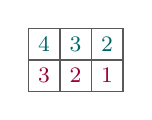
\begin{tikzpicture}[baseline={(0,-0.48)}]
\draw[gray!70!black,line width=0.5pt] (0,0) -- (0.4,0) -- (0.4,-0.4) -- (0,-0.4) -- cycle;
\draw[gray!70!black,line width=0.5pt] (0.4,0) -- (0.8,0) -- (0.8,-0.4) -- (0.4,-0.4) -- cycle;
\draw[gray!70!black,line width=0.5pt] (0.8,0) -- (1.2,0) -- (1.2,-0.4) -- (0.8,-0.4) -- cycle;
\draw[gray!70!black,line width=0.5pt] (0,-0.4) -- (0.4,-0.4) -- (0.4,-0.8) -- (0,-0.8) -- cycle;
\draw[gray!70!black,line width=0.5pt] (0.4,-0.4) -- (0.8,-0.4) -- (0.8,-0.8) -- (0.4,-0.8) -- cycle;
\draw[gray!70!black,line width=0.5pt] (0.8,-0.4) -- (1.2,-0.4) -- (1.2,-0.8) -- (0.8,-0.8) -- cycle;
\node[font=\footnotesize,inner sep=0pt,text=cLeft] at (0.2,-0.2) {$4$};
\node[font=\footnotesize,inner sep=0pt,text=cLeft] at (0.6,-0.2) {$3$};
\node[font=\footnotesize,inner sep=0pt,text=cLeft] at (1,-0.2) {$2$};
\node[font=\footnotesize,inner sep=0pt,text=cRight] at (0.2,-0.6) {$3$};
\node[font=\footnotesize,inner sep=0pt,text=cRight] at (0.6,-0.6) {$2$};
\node[font=\footnotesize,inner sep=0pt,text=cRight] at (1,-0.6) {$1$};
\end{tikzpicture}}

\newcommand{\FigMXIIICorner}{%
\begin{tikzpicture}
\fill[cC!30] (0.72,-0.37) -- (1.08,-0.37) -- (1.08,-0.73) -- (0.72,-0.73) -- cycle;
\fill[cC!30] (0.36,-0.73) -- (0.72,-0.73) -- (0.72,-1.09) -- (0.36,-1.09) -- cycle;
\draw[gray!70!black,line width=0.5pt] (0,-0.37) -- (0.36,-0.37) -- (0.36,-0.73) -- (0,-0.73) -- cycle;
\draw[gray!70!black,line width=0.5pt] (0.36,-0.37) -- (0.72,-0.37) -- (0.72,-0.73) -- (0.36,-0.73) -- cycle;
\draw[gray!70!black,line width=0.5pt] (0.72,-0.37) -- (1.08,-0.37) -- (1.08,-0.73) -- (0.72,-0.73) -- cycle;
\draw[gray!70!black,line width=0.5pt] (0,-0.73) -- (0.36,-0.73) -- (0.36,-1.09) -- (0,-1.09) -- cycle;
\draw[gray!70!black,line width=0.5pt] (0.36,-0.73) -- (0.72,-0.73) -- (0.72,-1.09) -- (0.36,-1.09) -- cycle;
\node[font=\footnotesize] at (0.54,-1.36) {$\lambda=(3,2)$};
\node[font=\scriptsize,text=cC!80!black] at (0.54,-0.15) {角落};
\fill[cC!30] (2.72,0.3) -- (3.08,0.3) -- (3.08,-0.06) -- (2.72,-0.06) -- cycle;
\draw[gray!70!black,line width=0.5pt] (2,0.3) -- (2.36,0.3) -- (2.36,-0.06) -- (2,-0.06) -- cycle;
\draw[gray!70!black,line width=0.5pt] (2.36,0.3) -- (2.72,0.3) -- (2.72,-0.06) -- (2.36,-0.06) -- cycle;
\draw[gray!70!black,line width=0.5pt] (2.72,0.3) -- (3.08,0.3) -- (3.08,-0.06) -- (2.72,-0.06) -- cycle;
\draw[gray!70!black,line width=0.5pt] (2,-0.06) -- (2.36,-0.06) -- (2.36,-0.42) -- (2,-0.42) -- cycle;
\draw[gray!70!black,line width=0.5pt] (2.36,-0.06) -- (2.72,-0.06) -- (2.72,-0.42) -- (2.36,-0.42) -- cycle;
\node[font=\scriptsize,inner sep=0pt] at (2.18,0.12) {$1$};
\node[font=\scriptsize,inner sep=0pt] at (2.54,0.12) {$2$};
\node[font=\scriptsize,inner sep=0pt] at (2.9,0.12) {$5$};
\node[font=\scriptsize,inner sep=0pt] at (2.18,-0.24) {$3$};
\node[font=\scriptsize,inner sep=0pt] at (2.54,-0.24) {$4$};
\fill[cC!30] (4.1,0.3) -- (4.46,0.3) -- (4.46,-0.06) -- (4.1,-0.06) -- cycle;
\draw[gray!70!black,line width=0.5pt] (3.38,0.3) -- (3.74,0.3) -- (3.74,-0.06) -- (3.38,-0.06) -- cycle;
\draw[gray!70!black,line width=0.5pt] (3.74,0.3) -- (4.1,0.3) -- (4.1,-0.06) -- (3.74,-0.06) -- cycle;
\draw[gray!70!black,line width=0.5pt] (4.1,0.3) -- (4.46,0.3) -- (4.46,-0.06) -- (4.1,-0.06) -- cycle;
\draw[gray!70!black,line width=0.5pt] (3.38,-0.06) -- (3.74,-0.06) -- (3.74,-0.42) -- (3.38,-0.42) -- cycle;
\draw[gray!70!black,line width=0.5pt] (3.74,-0.06) -- (4.1,-0.06) -- (4.1,-0.42) -- (3.74,-0.42) -- cycle;
\node[font=\scriptsize,inner sep=0pt] at (3.56,0.12) {$1$};
\node[font=\scriptsize,inner sep=0pt] at (3.92,0.12) {$3$};
\node[font=\scriptsize,inner sep=0pt] at (4.28,0.12) {$5$};
\node[font=\scriptsize,inner sep=0pt] at (3.56,-0.24) {$2$};
\node[font=\scriptsize,inner sep=0pt] at (3.92,-0.24) {$4$};
\draw[-{Stealth[length=5pt]},gray!60!black,line width=0.7pt] (6.19,-0.06) -- (7.24,-0.06) node[midway,above,font=\footnotesize,text=black] {拿掉 $5$};
\draw[gray!70!black,line width=0.5pt] (7.49,0.3) -- (7.85,0.3) -- (7.85,-0.06) -- (7.49,-0.06) -- cycle;
\draw[gray!70!black,line width=0.5pt] (7.85,0.3) -- (8.21,0.3) -- (8.21,-0.06) -- (7.85,-0.06) -- cycle;
\draw[gray!70!black,line width=0.5pt] (7.49,-0.06) -- (7.85,-0.06) -- (7.85,-0.42) -- (7.49,-0.42) -- cycle;
\draw[gray!70!black,line width=0.5pt] (7.85,-0.06) -- (8.21,-0.06) -- (8.21,-0.42) -- (7.85,-0.42) -- cycle;
\node[anchor=west,font=\small] at (8.51,-0.06) {$f^{(2,2)}=2$};
\fill[cC!30] (2.36,-1.41) -- (2.72,-1.41) -- (2.72,-1.77) -- (2.36,-1.77) -- cycle;
\draw[gray!70!black,line width=0.5pt] (2,-1.05) -- (2.36,-1.05) -- (2.36,-1.41) -- (2,-1.41) -- cycle;
\draw[gray!70!black,line width=0.5pt] (2.36,-1.05) -- (2.72,-1.05) -- (2.72,-1.41) -- (2.36,-1.41) -- cycle;
\draw[gray!70!black,line width=0.5pt] (2.72,-1.05) -- (3.08,-1.05) -- (3.08,-1.41) -- (2.72,-1.41) -- cycle;
\draw[gray!70!black,line width=0.5pt] (2,-1.41) -- (2.36,-1.41) -- (2.36,-1.77) -- (2,-1.77) -- cycle;
\draw[gray!70!black,line width=0.5pt] (2.36,-1.41) -- (2.72,-1.41) -- (2.72,-1.77) -- (2.36,-1.77) -- cycle;
\node[font=\scriptsize,inner sep=0pt] at (2.18,-1.23) {$1$};
\node[font=\scriptsize,inner sep=0pt] at (2.54,-1.23) {$2$};
\node[font=\scriptsize,inner sep=0pt] at (2.9,-1.23) {$3$};
\node[font=\scriptsize,inner sep=0pt] at (2.18,-1.59) {$4$};
\node[font=\scriptsize,inner sep=0pt] at (2.54,-1.59) {$5$};
\fill[cC!30] (3.74,-1.41) -- (4.1,-1.41) -- (4.1,-1.77) -- (3.74,-1.77) -- cycle;
\draw[gray!70!black,line width=0.5pt] (3.38,-1.05) -- (3.74,-1.05) -- (3.74,-1.41) -- (3.38,-1.41) -- cycle;
\draw[gray!70!black,line width=0.5pt] (3.74,-1.05) -- (4.1,-1.05) -- (4.1,-1.41) -- (3.74,-1.41) -- cycle;
\draw[gray!70!black,line width=0.5pt] (4.1,-1.05) -- (4.46,-1.05) -- (4.46,-1.41) -- (4.1,-1.41) -- cycle;
\draw[gray!70!black,line width=0.5pt] (3.38,-1.41) -- (3.74,-1.41) -- (3.74,-1.77) -- (3.38,-1.77) -- cycle;
\draw[gray!70!black,line width=0.5pt] (3.74,-1.41) -- (4.1,-1.41) -- (4.1,-1.77) -- (3.74,-1.77) -- cycle;
\node[font=\scriptsize,inner sep=0pt] at (3.56,-1.23) {$1$};
\node[font=\scriptsize,inner sep=0pt] at (3.92,-1.23) {$2$};
\node[font=\scriptsize,inner sep=0pt] at (4.28,-1.23) {$4$};
\node[font=\scriptsize,inner sep=0pt] at (3.56,-1.59) {$3$};
\node[font=\scriptsize,inner sep=0pt] at (3.92,-1.59) {$5$};
\fill[cC!30] (5.12,-1.41) -- (5.48,-1.41) -- (5.48,-1.77) -- (5.12,-1.77) -- cycle;
\draw[gray!70!black,line width=0.5pt] (4.76,-1.05) -- (5.12,-1.05) -- (5.12,-1.41) -- (4.76,-1.41) -- cycle;
\draw[gray!70!black,line width=0.5pt] (5.12,-1.05) -- (5.48,-1.05) -- (5.48,-1.41) -- (5.12,-1.41) -- cycle;
\draw[gray!70!black,line width=0.5pt] (5.48,-1.05) -- (5.84,-1.05) -- (5.84,-1.41) -- (5.48,-1.41) -- cycle;
\draw[gray!70!black,line width=0.5pt] (4.76,-1.41) -- (5.12,-1.41) -- (5.12,-1.77) -- (4.76,-1.77) -- cycle;
\draw[gray!70!black,line width=0.5pt] (5.12,-1.41) -- (5.48,-1.41) -- (5.48,-1.77) -- (5.12,-1.77) -- cycle;
\node[font=\scriptsize,inner sep=0pt] at (4.94,-1.23) {$1$};
\node[font=\scriptsize,inner sep=0pt] at (5.3,-1.23) {$3$};
\node[font=\scriptsize,inner sep=0pt] at (5.66,-1.23) {$4$};
\node[font=\scriptsize,inner sep=0pt] at (4.94,-1.59) {$2$};
\node[font=\scriptsize,inner sep=0pt] at (5.3,-1.59) {$5$};
\draw[-{Stealth[length=5pt]},gray!60!black,line width=0.7pt] (6.19,-1.41) -- (7.24,-1.41) node[midway,above,font=\footnotesize,text=black] {拿掉 $5$};
\draw[gray!70!black,line width=0.5pt] (7.49,-1.05) -- (7.85,-1.05) -- (7.85,-1.41) -- (7.49,-1.41) -- cycle;
\draw[gray!70!black,line width=0.5pt] (7.85,-1.05) -- (8.21,-1.05) -- (8.21,-1.41) -- (7.85,-1.41) -- cycle;
\draw[gray!70!black,line width=0.5pt] (8.21,-1.05) -- (8.57,-1.05) -- (8.57,-1.41) -- (8.21,-1.41) -- cycle;
\draw[gray!70!black,line width=0.5pt] (7.49,-1.41) -- (7.85,-1.41) -- (7.85,-1.77) -- (7.49,-1.77) -- cycle;
\node[anchor=west,font=\small] at (8.87,-1.41) {$f^{(3,1)}=3$};
\end{tikzpicture}}

\newcommand{\FigMXIVWalks}{%
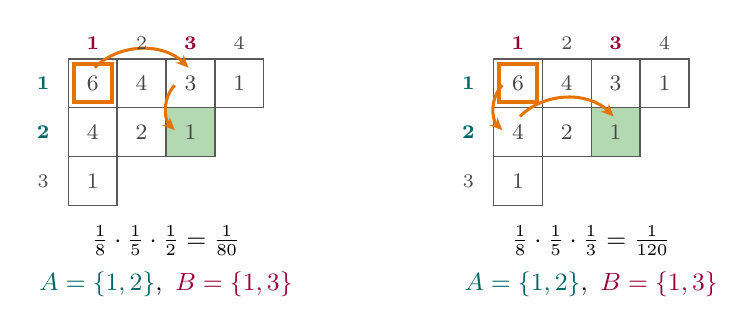
\begin{tikzpicture}
\fill[cC!30] (1.24,-0.62) -- (1.86,-0.62) -- (1.86,-1.24) -- (1.24,-1.24) -- cycle;
\draw[gray!70!black,line width=0.5pt] (0,0) -- (0.62,0) -- (0.62,-0.62) -- (0,-0.62) -- cycle;
\draw[gray!70!black,line width=0.5pt] (0.62,0) -- (1.24,0) -- (1.24,-0.62) -- (0.62,-0.62) -- cycle;
\draw[gray!70!black,line width=0.5pt] (1.24,0) -- (1.86,0) -- (1.86,-0.62) -- (1.24,-0.62) -- cycle;
\draw[gray!70!black,line width=0.5pt] (1.86,0) -- (2.48,0) -- (2.48,-0.62) -- (1.86,-0.62) -- cycle;
\draw[gray!70!black,line width=0.5pt] (0,-0.62) -- (0.62,-0.62) -- (0.62,-1.24) -- (0,-1.24) -- cycle;
\draw[gray!70!black,line width=0.5pt] (0.62,-0.62) -- (1.24,-0.62) -- (1.24,-1.24) -- (0.62,-1.24) -- cycle;
\draw[gray!70!black,line width=0.5pt] (1.24,-0.62) -- (1.86,-0.62) -- (1.86,-1.24) -- (1.24,-1.24) -- cycle;
\draw[gray!70!black,line width=0.5pt] (0,-1.24) -- (0.62,-1.24) -- (0.62,-1.86) -- (0,-1.86) -- cycle;
\node[font=\footnotesize,inner sep=0pt,text=gray!55!black] at (0.31,-0.31) {$6$};
\node[font=\footnotesize,inner sep=0pt,text=gray!55!black] at (0.93,-0.31) {$4$};
\node[font=\footnotesize,inner sep=0pt,text=gray!55!black] at (1.55,-0.31) {$3$};
\node[font=\footnotesize,inner sep=0pt,text=gray!55!black] at (2.17,-0.31) {$1$};
\node[font=\footnotesize,inner sep=0pt,text=gray!55!black] at (0.31,-0.93) {$4$};
\node[font=\footnotesize,inner sep=0pt,text=gray!55!black] at (0.93,-0.93) {$2$};
\node[font=\footnotesize,inner sep=0pt,text=gray!55!black] at (1.55,-0.93) {$1$};
\node[font=\footnotesize,inner sep=0pt,text=gray!55!black] at (0.31,-1.55) {$1$};
\draw[cTop,line width=1.4pt] (0.07,-0.07) rectangle (0.55,-0.55);
\draw[-{Stealth[length=4.5pt,width=4pt]},cTop,line width=1.1pt,shorten <=1pt,shorten >=1pt] (0.31,-0.136) to[bend left=45] (1.55,-0.136);
\draw[-{Stealth[length=4.5pt,width=4pt]},cTop,line width=1.1pt,shorten <=1pt,shorten >=1pt] (1.376,-0.31) to[bend right=45] (1.376,-0.93);
\node[font=\scriptsize\bfseries,text=cLeft] at (-0.32,-0.31) {1};
\node[font=\scriptsize\bfseries,text=cLeft] at (-0.32,-0.93) {2};
\node[font=\scriptsize,text=gray!60!black] at (-0.32,-1.55) {3};
\node[font=\scriptsize\bfseries,text=cRight] at (0.31,0.2) {1};
\node[font=\scriptsize,text=gray!60!black] at (0.93,0.2) {2};
\node[font=\scriptsize\bfseries,text=cRight] at (1.55,0.2) {3};
\node[font=\scriptsize,text=gray!60!black] at (2.17,0.2) {4};
\node[font=\small] at (1.24,-2.31) {$\frac{1}{8}\cdot\frac{1}{5}\cdot\frac{1}{2}=\frac{1}{80}$};
\node[font=\small] at (1.24,-2.86) {$\textcolor{cLeft}{A=\{1,2\}},\ \textcolor{cRight}{B=\{1,3\}}$};
\fill[cC!30] (6.64,-0.62) -- (7.26,-0.62) -- (7.26,-1.24) -- (6.64,-1.24) -- cycle;
\draw[gray!70!black,line width=0.5pt] (5.4,0) -- (6.02,0) -- (6.02,-0.62) -- (5.4,-0.62) -- cycle;
\draw[gray!70!black,line width=0.5pt] (6.02,0) -- (6.64,0) -- (6.64,-0.62) -- (6.02,-0.62) -- cycle;
\draw[gray!70!black,line width=0.5pt] (6.64,0) -- (7.26,0) -- (7.26,-0.62) -- (6.64,-0.62) -- cycle;
\draw[gray!70!black,line width=0.5pt] (7.26,0) -- (7.88,0) -- (7.88,-0.62) -- (7.26,-0.62) -- cycle;
\draw[gray!70!black,line width=0.5pt] (5.4,-0.62) -- (6.02,-0.62) -- (6.02,-1.24) -- (5.4,-1.24) -- cycle;
\draw[gray!70!black,line width=0.5pt] (6.02,-0.62) -- (6.64,-0.62) -- (6.64,-1.24) -- (6.02,-1.24) -- cycle;
\draw[gray!70!black,line width=0.5pt] (6.64,-0.62) -- (7.26,-0.62) -- (7.26,-1.24) -- (6.64,-1.24) -- cycle;
\draw[gray!70!black,line width=0.5pt] (5.4,-1.24) -- (6.02,-1.24) -- (6.02,-1.86) -- (5.4,-1.86) -- cycle;
\node[font=\footnotesize,inner sep=0pt,text=gray!55!black] at (5.71,-0.31) {$6$};
\node[font=\footnotesize,inner sep=0pt,text=gray!55!black] at (6.33,-0.31) {$4$};
\node[font=\footnotesize,inner sep=0pt,text=gray!55!black] at (6.95,-0.31) {$3$};
\node[font=\footnotesize,inner sep=0pt,text=gray!55!black] at (7.57,-0.31) {$1$};
\node[font=\footnotesize,inner sep=0pt,text=gray!55!black] at (5.71,-0.93) {$4$};
\node[font=\footnotesize,inner sep=0pt,text=gray!55!black] at (6.33,-0.93) {$2$};
\node[font=\footnotesize,inner sep=0pt,text=gray!55!black] at (6.95,-0.93) {$1$};
\node[font=\footnotesize,inner sep=0pt,text=gray!55!black] at (5.71,-1.55) {$1$};
\draw[cTop,line width=1.4pt] (5.47,-0.07) rectangle (5.95,-0.55);
\draw[-{Stealth[length=4.5pt,width=4pt]},cTop,line width=1.1pt,shorten <=1pt,shorten >=1pt] (5.536,-0.31) to[bend right=45] (5.536,-0.93);
\draw[-{Stealth[length=4.5pt,width=4pt]},cTop,line width=1.1pt,shorten <=1pt,shorten >=1pt] (5.71,-0.756) to[bend left=45] (6.95,-0.756);
\node[font=\scriptsize\bfseries,text=cLeft] at (5.08,-0.31) {1};
\node[font=\scriptsize\bfseries,text=cLeft] at (5.08,-0.93) {2};
\node[font=\scriptsize,text=gray!60!black] at (5.08,-1.55) {3};
\node[font=\scriptsize\bfseries,text=cRight] at (5.71,0.2) {1};
\node[font=\scriptsize,text=gray!60!black] at (6.33,0.2) {2};
\node[font=\scriptsize\bfseries,text=cRight] at (6.95,0.2) {3};
\node[font=\scriptsize,text=gray!60!black] at (7.57,0.2) {4};
\node[font=\small] at (6.64,-2.31) {$\frac{1}{8}\cdot\frac{1}{5}\cdot\frac{1}{3}=\frac{1}{120}$};
\node[font=\small] at (6.64,-2.86) {$\textcolor{cLeft}{A=\{1,2\}},\ \textcolor{cRight}{B=\{1,3\}}$};
\end{tikzpicture}}

\newcommand{\FigMXIVIdentity}{%
\begin{tikzpicture}
\fill[yellow!55] (0.42,0) -- (0.84,0) -- (0.84,-0.42) -- (0.42,-0.42) -- cycle;
\fill[yellow!55] (0.84,0) -- (1.26,0) -- (1.26,-0.42) -- (0.84,-0.42) -- cycle;
\fill[yellow!55] (1.26,0) -- (1.68,0) -- (1.68,-0.42) -- (1.26,-0.42) -- cycle;
\fill[yellow!55] (0,-0.42) -- (0.42,-0.42) -- (0.42,-0.84) -- (0,-0.84) -- cycle;
\fill[yellow!55] (0,-0.84) -- (0.42,-0.84) -- (0.42,-1.26) -- (0,-1.26) -- cycle;
\draw[gray!70!black,line width=0.5pt] (0,0) -- (0.42,0) -- (0.42,-0.42) -- (0,-0.42) -- cycle;
\draw[gray!70!black,line width=0.5pt] (0.42,0) -- (0.84,0) -- (0.84,-0.42) -- (0.42,-0.42) -- cycle;
\draw[gray!70!black,line width=0.5pt] (0.84,0) -- (1.26,0) -- (1.26,-0.42) -- (0.84,-0.42) -- cycle;
\draw[gray!70!black,line width=0.5pt] (1.26,0) -- (1.68,0) -- (1.68,-0.42) -- (1.26,-0.42) -- cycle;
\draw[gray!70!black,line width=0.5pt] (0,-0.42) -- (0.42,-0.42) -- (0.42,-0.84) -- (0,-0.84) -- cycle;
\draw[gray!70!black,line width=0.5pt] (0.42,-0.42) -- (0.84,-0.42) -- (0.84,-0.84) -- (0.42,-0.84) -- cycle;
\draw[gray!70!black,line width=0.5pt] (0.84,-0.42) -- (1.26,-0.42) -- (1.26,-0.84) -- (0.84,-0.84) -- cycle;
\draw[gray!70!black,line width=0.5pt] (0,-0.84) -- (0.42,-0.84) -- (0.42,-1.26) -- (0,-1.26) -- cycle;
\draw[cTop,line width=1.3pt] (0.06,-0.06) rectangle (0.36,-0.36);
\draw[cC,line width=1.3pt,densely dashed] (0.9,-0.48) rectangle (1.2,-0.78);
\node[font=\small] at (0.84,0.32) {$h(a,b)-1$};
\node[font=\normalsize] at (0.84,-1.58) {$5$};
\fill[cLeft!35] (4.01,0) -- (4.43,0) -- (4.43,-0.42) -- (4.01,-0.42) -- cycle;
\fill[cLeft!35] (3.59,-0.42) -- (4.01,-0.42) -- (4.01,-0.84) -- (3.59,-0.84) -- cycle;
\draw[gray!70!black,line width=0.5pt] (2.75,0) -- (3.17,0) -- (3.17,-0.42) -- (2.75,-0.42) -- cycle;
\draw[gray!70!black,line width=0.5pt] (3.17,0) -- (3.59,0) -- (3.59,-0.42) -- (3.17,-0.42) -- cycle;
\draw[gray!70!black,line width=0.5pt] (3.59,0) -- (4.01,0) -- (4.01,-0.42) -- (3.59,-0.42) -- cycle;
\draw[gray!70!black,line width=0.5pt] (4.01,0) -- (4.43,0) -- (4.43,-0.42) -- (4.01,-0.42) -- cycle;
\draw[gray!70!black,line width=0.5pt] (2.75,-0.42) -- (3.17,-0.42) -- (3.17,-0.84) -- (2.75,-0.84) -- cycle;
\draw[gray!70!black,line width=0.5pt] (3.17,-0.42) -- (3.59,-0.42) -- (3.59,-0.84) -- (3.17,-0.84) -- cycle;
\draw[gray!70!black,line width=0.5pt] (3.59,-0.42) -- (4.01,-0.42) -- (4.01,-0.84) -- (3.59,-0.84) -- cycle;
\draw[gray!70!black,line width=0.5pt] (2.75,-0.84) -- (3.17,-0.84) -- (3.17,-1.26) -- (2.75,-1.26) -- cycle;
\draw[cTop,line width=1.3pt] (3.65,-0.06) rectangle (3.95,-0.36);
\draw[cC,line width=1.3pt,densely dashed] (3.65,-0.48) rectangle (3.95,-0.78);
\node[font=\small] at (3.59,0.32) {$h(a,\beta)-1$};
\node[font=\normalsize] at (3.59,-1.58) {$2$};
\fill[cRight!30] (5.92,-0.42) -- (6.34,-0.42) -- (6.34,-0.84) -- (5.92,-0.84) -- cycle;
\fill[cRight!30] (6.34,-0.42) -- (6.76,-0.42) -- (6.76,-0.84) -- (6.34,-0.84) -- cycle;
\fill[cRight!30] (5.5,-0.84) -- (5.92,-0.84) -- (5.92,-1.26) -- (5.5,-1.26) -- cycle;
\draw[gray!70!black,line width=0.5pt] (5.5,0) -- (5.92,0) -- (5.92,-0.42) -- (5.5,-0.42) -- cycle;
\draw[gray!70!black,line width=0.5pt] (5.92,0) -- (6.34,0) -- (6.34,-0.42) -- (5.92,-0.42) -- cycle;
\draw[gray!70!black,line width=0.5pt] (6.34,0) -- (6.76,0) -- (6.76,-0.42) -- (6.34,-0.42) -- cycle;
\draw[gray!70!black,line width=0.5pt] (6.76,0) -- (7.18,0) -- (7.18,-0.42) -- (6.76,-0.42) -- cycle;
\draw[gray!70!black,line width=0.5pt] (5.5,-0.42) -- (5.92,-0.42) -- (5.92,-0.84) -- (5.5,-0.84) -- cycle;
\draw[gray!70!black,line width=0.5pt] (5.92,-0.42) -- (6.34,-0.42) -- (6.34,-0.84) -- (5.92,-0.84) -- cycle;
\draw[gray!70!black,line width=0.5pt] (6.34,-0.42) -- (6.76,-0.42) -- (6.76,-0.84) -- (6.34,-0.84) -- cycle;
\draw[gray!70!black,line width=0.5pt] (5.5,-0.84) -- (5.92,-0.84) -- (5.92,-1.26) -- (5.5,-1.26) -- cycle;
\draw[cTop,line width=1.3pt] (5.56,-0.48) rectangle (5.86,-0.78);
\draw[cC,line width=1.3pt,densely dashed] (6.4,-0.48) rectangle (6.7,-0.78);
\node[font=\small] at (6.34,0.32) {$h(\alpha,b)-1$};
\node[font=\normalsize] at (6.34,-1.58) {$3$};
\node[font=\large] at (2.215,-0.63) {$=$};
\node[font=\large] at (4.965,-0.63) {$+$};
\end{tikzpicture}}

\newcommand{\FigMXIVRemove}{%
\begin{tikzpicture}
\fill[cLeft!30] (1.1,0) -- (1.65,0) -- (1.65,-0.55) -- (1.1,-0.55) -- cycle;
\fill[cRight!28] (0,-0.55) -- (0.55,-0.55) -- (0.55,-1.1) -- (0,-1.1) -- cycle;
\fill[cRight!28] (0.55,-0.55) -- (1.1,-0.55) -- (1.1,-1.1) -- (0.55,-1.1) -- cycle;
\fill[cC!30] (1.1,-0.55) -- (1.65,-0.55) -- (1.65,-1.1) -- (1.1,-1.1) -- cycle;
\draw[gray!70!black,line width=0.5pt] (0,0) -- (0.55,0) -- (0.55,-0.55) -- (0,-0.55) -- cycle;
\draw[gray!70!black,line width=0.5pt] (0.55,0) -- (1.1,0) -- (1.1,-0.55) -- (0.55,-0.55) -- cycle;
\draw[gray!70!black,line width=0.5pt] (1.1,0) -- (1.65,0) -- (1.65,-0.55) -- (1.1,-0.55) -- cycle;
\draw[gray!70!black,line width=0.5pt] (1.65,0) -- (2.2,0) -- (2.2,-0.55) -- (1.65,-0.55) -- cycle;
\draw[gray!70!black,line width=0.5pt] (0,-0.55) -- (0.55,-0.55) -- (0.55,-1.1) -- (0,-1.1) -- cycle;
\draw[gray!70!black,line width=0.5pt] (0.55,-0.55) -- (1.1,-0.55) -- (1.1,-1.1) -- (0.55,-1.1) -- cycle;
\draw[gray!70!black,line width=0.5pt] (1.1,-0.55) -- (1.65,-0.55) -- (1.65,-1.1) -- (1.1,-1.1) -- cycle;
\draw[gray!70!black,line width=0.5pt] (0,-1.1) -- (0.55,-1.1) -- (0.55,-1.65) -- (0,-1.65) -- cycle;
\node[font=\small,inner sep=0pt] at (0.275,-0.275) {$6$};
\node[font=\small,inner sep=0pt] at (0.825,-0.275) {$4$};
\node[font=\small,inner sep=0pt] at (1.375,-0.275) {$3$};
\node[font=\small,inner sep=0pt] at (1.925,-0.275) {$1$};
\node[font=\small,inner sep=0pt] at (0.275,-0.825) {$4$};
\node[font=\small,inner sep=0pt] at (0.825,-0.825) {$2$};
\node[font=\small,inner sep=0pt] at (1.375,-0.825) {$1$};
\node[font=\small,inner sep=0pt] at (0.275,-1.375) {$1$};
\fill[cLeft!30] (5.3,0) -- (5.85,0) -- (5.85,-0.55) -- (5.3,-0.55) -- cycle;
\fill[cRight!28] (4.2,-0.55) -- (4.75,-0.55) -- (4.75,-1.1) -- (4.2,-1.1) -- cycle;
\fill[cRight!28] (4.75,-0.55) -- (5.3,-0.55) -- (5.3,-1.1) -- (4.75,-1.1) -- cycle;
\draw[gray!70!black,line width=0.5pt] (4.2,0) -- (4.75,0) -- (4.75,-0.55) -- (4.2,-0.55) -- cycle;
\draw[gray!70!black,line width=0.5pt] (4.75,0) -- (5.3,0) -- (5.3,-0.55) -- (4.75,-0.55) -- cycle;
\draw[gray!70!black,line width=0.5pt] (5.3,0) -- (5.85,0) -- (5.85,-0.55) -- (5.3,-0.55) -- cycle;
\draw[gray!70!black,line width=0.5pt] (5.85,0) -- (6.4,0) -- (6.4,-0.55) -- (5.85,-0.55) -- cycle;
\draw[gray!70!black,line width=0.5pt] (4.2,-0.55) -- (4.75,-0.55) -- (4.75,-1.1) -- (4.2,-1.1) -- cycle;
\draw[gray!70!black,line width=0.5pt] (4.75,-0.55) -- (5.3,-0.55) -- (5.3,-1.1) -- (4.75,-1.1) -- cycle;
\draw[gray!70!black,line width=0.5pt] (4.2,-1.1) -- (4.75,-1.1) -- (4.75,-1.65) -- (4.2,-1.65) -- cycle;
\node[font=\small,inner sep=0pt] at (4.475,-0.275) {$6$};
\node[font=\small,inner sep=0pt] at (5.025,-0.275) {$4$};
\node[font=\small,inner sep=0pt] at (5.575,-0.275) {$2$};
\node[font=\small,inner sep=0pt] at (6.125,-0.275) {$1$};
\node[font=\small,inner sep=0pt] at (4.475,-0.825) {$3$};
\node[font=\small,inner sep=0pt] at (5.025,-0.825) {$1$};
\node[font=\small,inner sep=0pt] at (4.475,-1.375) {$1$};
\draw[gray!60,densely dashed,line width=0.6pt] (5.3,-0.55) rectangle (5.85,-1.1);
\draw[-{Stealth[length=5pt]},gray!60!black,line width=0.7pt] (2.55,-0.825) -- (3.85,-0.825) node[midway,above,font=\footnotesize,text=black] {拿掉 $c$};
\node[font=\small] at (1.1,0.3) {$\lambda=(4,3,1)$};
\node[font=\small] at (1.1,-1.95) {$H(\lambda)=576$};
\node[font=\small] at (5.3,0.3) {$\lambda-c=(4,2,1)$};
\node[font=\small] at (5.3,-1.95) {$H(\lambda-c)=144$};
\end{tikzpicture}}


% ---------------------------------------------------------------------
\subsection{標準 Young 表與 Dyck 路徑}\label{sec:m12}

這一節看兩列等長的形狀 $(n,n)$：它的標準 Young 表就是 Dyck 路徑 \mitref{L4}。
回憶第~\ref{sec:m11} 節的\textbf{標準 Young 表}：把 $1,2,\ldots,|\lambda|$（$|\lambda|$ 是格子數）各填一次到形狀 $\lambda$ 的 Young 圖，
每一列由左到右、每一行由上到下都遞增；個數記為 $f^{\lambda}$。

\textbf{讀表的規則。}依序讀 $1,2,\ldots,2n$：數字 $i$ 在第一列，第 $i$ 步就往上（U）；
在第二列，第 $i$ 步就往下（D）。貫穿的例子：第一列是 $1,2,4$、第二列是 $3,5,6$，
所以第 1、2、4 步是 U，第 3、5、6 步是 D，得到 UUDUDD（圖~\ref{fig:m12-convert}）。

\begin{figure}[H]
\centering
\FigMXIIConvert
\caption{形狀 $(3,3)$ 的表：\textcolor{cLeft}{第一列的數 $\to$ U}、\textcolor{cRight}{第二列的數 $\to$ D}。
例子 $\begin{smallmatrix}1&2&4\\3&5&6\end{smallmatrix}$ 變成 Dyck 路徑 UUDUDD。}
\label{fig:m12-convert}
\end{figure}

\textbf{為什麼不會掉到地面以下。}記 $T_{r,j}$ 為第 $r$ 列第 $j$ 格的數。
列是遞增的，所以第 $j$ 個 U 是第 $T_{1,j}$ 步，第 $j$ 個 D 是第 $T_{2,j}$ 步。
行也是遞增的：$T_{1,j}<T_{2,j}$，也就是\textbf{第 $j$ 個 D 之前，一定已經有第 $j$ 個 U}。
所以任何時候 U 的個數都 $\ge$ D 的個數，路徑不低於地面。例子的三行是 $1<3$、$2<5$、$4<6$。

\textbf{反過來。}給一條半長 $n$ 的 Dyck 路徑，把 U 所在的步號由小到大填進第一列、D 所在的步號填進第二列。
兩列自動遞增；路徑不低於地面，表示第 $j$ 個 U 比第 $j$ 個 D 早，也就是每一行遞增。
兩個方向互為反函數，所以是一一對應。

\begin{thmbox}[兩列的標準 Young 表]
形狀 $(n,n)$ 的標準 Young 表與半長 $n$ 的 Dyck 路徑一一對應，所以 $f^{(n,n)}=C_n$。
\end{thmbox}

\begin{figure}[H]
\centering
\FigMXIIAll
\caption{形狀 $(3,3)$ 的 5 個標準 Young 表與對應的 5 條 Dyck 路徑（順序同動畫 M12），
\textcolor{cTop}{虛線框}是貫穿的例子。}
\label{fig:m12-all}
\end{figure}

程式逐一列舉 $n=1,\ldots,6$：$f^{(n,n)}=1,2,5,14,42,132$，與 $C_n$ 相同。
換成投票問題的語言（圖~\ref{fig:ballot}）：第 $i$ 張票投給 A 就把 $i$ 放進第一列、投給 B 就放進第二列，
「行遞增」就是「A 從不落後」；例子對應開票順序 AABABB。

\textbf{一般的形狀。}$\lambda=(\lambda_1,\ldots,\lambda_k)$ 有 $k$ 列。
數字 $i$ 在第 $r$ 列，第 $i$ 步就走 $e_r$（第 $r$ 個座標加 1）。
讀完前 $t$ 個數之後的位置 $(x_1,\ldots,x_k)$，就是各列已經填了幾格。
第 $r$ 列要填第 $j$ 格時，它上面那格（第 $r-1$ 列第 $j$ 格）必須早就填好，也就是填完之後仍有 $x_{r-1}\ge x_r$。
所以「每一行遞增」等於\textbf{一路上都保持 $x_1\ge x_2\ge\cdots\ge x_k$}（表~\ref{tab:m12-general}）。

\begin{thmbox}[標準 Young 表 $=$ 格子路徑]
形狀 $\lambda$ 的標準 Young 表，一一對應到 $\mathbb{Z}^k$ 中從原點走到 $\lambda$、每一步是某個 $e_r$、
一路保持 $x_1\ge x_2\ge\cdots\ge x_k$ 的格子路徑。
$\lambda=(n,n)$ 時，$x_1\ge x_2$ 就是「U 不比 D 少」，回到 Dyck 路徑。
\end{thmbox}

\begin{table}[H]
\centering
\small
\renewcommand{\arraystretch}{1.15}
\begin{tabular}{@{}c@{\qquad}cccccl@{}}
\toprule
表 & 讀完 1 & 讀完 2 & 讀完 3 & 讀完 4 & 讀完 5 & \\
\midrule
\FigMXIIGenGood & $(1,0,0)$ & $(1,1,0)$ & $(2,1,0)$ & $(2,1,1)$ & $(2,2,1)$ & 一路 $x_1\ge x_2\ge x_3$ \\[0.5em]
\FigMXIIGenBad & $(1,0,0)$ & $(1,1,0)$ & $(1,1,1)$ & $\textcolor{cBad}{(1,2,1)}$ & $(2,2,1)$
  & \textcolor{cBad}{$x_2>x_1$，不是標準 Young 表}\\
\bottomrule
\end{tabular}
\caption{形狀 $\lambda=(2,2,1)$。上：依序走 $e_1,e_2,e_1,e_3,e_2$，每一步都有 $x_1\ge x_2\ge x_3$，終點是 $\lambda$。
下：把 5 放在 4 上面（\textcolor{cBad}{紅框}那一行 $5>4$），讀到 4 時 $x_2=2>x_1=1$，路徑跑出區域。}
\label{tab:m12-general}
\end{table}

% ---------------------------------------------------------------------
\subsection{鉤長公式}\label{sec:m13}

$f^{\lambda}$ 有一條漂亮的公式，只用到每一格的「鉤長」\mitref{L4}。

\textbf{鉤。}格子 $c$ 的\textbf{鉤}（hook）由三部分組成：$c$ 自己、同一列在它右邊的格子（\textbf{臂}，arm）、
同一行在它下面的格子（\textbf{腿}，leg）。鉤裡的格子數叫做\textbf{鉤長}：
\[
h(c)=\operatorname{arm}(c)+\operatorname{leg}(c)+1 .
\]
$c$ 在第 $i$ 列第 $j$ 行時，$\operatorname{arm}(c)=\lambda_i-j$、$\operatorname{leg}(c)=\lambda'_j-i$，
其中 $\lambda'_j$ 是第 $j$ 行的長度。例：$\lambda=(4,3,1)$ 的格子 $c=(1,2)$ 有 2 格臂、1 格腿，
$h(c)=4$（圖~\ref{fig:m13-hook} 左）。

\begin{figure}[H]
\centering
\FigMXIIIHook
\caption{$\lambda=(4,3,1)$。左：格子 $c=(1,2)$ 的鉤，由\textcolor{cTop}{橘色的 $c$ 自己}和黃色的臂、腿組成。右：每一格的鉤長。}
\label{fig:m13-hook}
\end{figure}

把每一格的鉤長乘起來：
\[
H(\lambda)=\prod_{c\in\lambda}h(c)=6\cdot4\cdot3\cdot1\cdot4\cdot2\cdot1\cdot1=576,\qquad
\frac{8!}{H(\lambda)}=\frac{40320}{576}=70 .
\]
而形狀 $(4,3,1)$ 的標準 Young 表恰有 70 個（程式列舉）。這不是巧合：

\begin{thmbox}[鉤長公式（Frame--Robinson--Thrall，1954）]
$\lambda$ 是 $n$ 的分割時，形狀 $\lambda$ 的標準 Young 表個數是
\begin{equation}\label{eq:m13-hook}
f^{\lambda}=\frac{n!}{\prod_{c\in\lambda}h(c)}=\frac{n!}{H(\lambda)} .
\end{equation}
\end{thmbox}

\textbf{驗算。}第~\ref{sec:m11} 節列出的 $(3,2)$，以及上一節的 $(3,3)$（格子裡是鉤長）：
\[
\FigMXIIIHookSmall\quad \frac{5!}{4\cdot3\cdot1\cdot2\cdot1}=\frac{120}{24}=5,
\qquad\qquad
\FigMXIIIHookSquare\quad \frac{6!}{(4\cdot3\cdot2)(3\cdot2\cdot1)}=\frac{720}{144}=5=C_3 .
\]
一般的 $(n,n)$：第一列的鉤長是 \textcolor{cLeft}{$n+1,n,\ldots,2$}，第二列是 \textcolor{cRight}{$n,n-1,\ldots,1$}，
所以 $H=(n+1)!\,n!$，
\[
f^{(n,n)}=\frac{(2n)!}{(n+1)!\,n!}=C_n ,
\]
這是 $f^{(n,n)}=C_n$ 的第二個證明。

\textbf{角落遞迴。}以下 $\lambda$ 是 $n$ 的分割。右邊和下面都沒有格子的格子叫\textbf{角落}；拿掉角落 $c$，剩下的 $\lambda-c$ 仍是 Young 圖。
在標準 Young 表裡，最大的數 $n$ 一定在某個角落：它右邊或下面的數都要比 $n$ 大，所以那裡不能有格子。
拿掉 $n$，剩下的是形狀 $\lambda-c$ 的標準 Young 表；反過來，在 $\lambda-c$ 的表的格子 $c$ 填上 $n$，
就得到 $\lambda$ 的表。所以
\begin{equation}\label{eq:m13-corner}
f^{\lambda}=\sum_{c\ \text{是角落}}f^{\lambda-c},\qquad f^{\varnothing}=1 .
\end{equation}
例：$(3,2)$ 的 5 個表依 5 的位置分成 $2+3$ 個（圖~\ref{fig:m13-corner}），
$f^{(3,2)}=f^{(2,2)}+f^{(3,1)}=2+3=5$。

\begin{figure}[H]
\centering
\FigMXIIICorner
\caption{角落遞迴：$(3,2)$ 的 5 個表依最大數 5 所在的\textcolor{cC}{角落}分成兩組，拿掉 5 就是較小形狀的表。}
\label{fig:m13-corner}
\end{figure}

\textbf{化約成「機率和為 1」。}令 $F(\lambda)=n!/H(\lambda)$。要證 $F=f$，對 $n$ 歸納：
$F(\varnothing)=1$，所以只要再證明 $F$ 也滿足角落遞迴 \eqref{eq:m13-corner}。
設 $n-1$ 格的形狀都已有 $f=F$，則 $f^{\lambda}=\sum_c F(\lambda-c)$，只需證 $\sum_c F(\lambda-c)=F(\lambda)$。
兩邊除以 $F(\lambda)$：
\begin{equation}\label{eq:m13-reduce}
\sum_{c}\frac{(n-1)!}{H(\lambda-c)}\cdot\frac{H(\lambda)}{n!}
=\sum_{c\ \text{是角落}}\frac{1}{n}\cdot\frac{H(\lambda)}{H(\lambda-c)}=1 .
\end{equation}
驗算 $(3,2)$：$H(3,2)=24$、$H(2,2)=12$、$H(3,1)=8$，
\[
\frac15\cdot\frac{24}{12}+\frac15\cdot\frac{24}{8}=\frac25+\frac35=1 .
\]
式 \eqref{eq:m13-reduce} 的每一項都是正的、加起來是 1，很像機率。
下一節的「鉤上漫步」讓它們真的變成機率：停在角落 $c$ 的機率。

% ---------------------------------------------------------------------
\subsection{鉤上漫步的證明}\label{sec:m14}

這一節用 Greene、Nijenhuis 與 Wilf（1979）的機率論證 \mitref{L4} 證明式 \eqref{eq:m13-reduce}，
於是得到鉤長公式。例子沿用 $\lambda=(4,3,1)$，$n=8$。格子 $(i,j)$ 指第 $i$ 列第 $j$ 行。

\textbf{(1) 鉤上漫步。}
\begin{enumerate}[leftmargin=1.6em]
  \item 從 $n$ 格中\textbf{均勻}隨機選一格當起點，每格機率 $\frac1n$。
  \item 在格子 $x$ 上，若 $h(x)>1$，就從 $x$ 的鉤上「$x$ 以外的 $h(x)-1$ 格」均勻選一格跳過去，
        每格機率 $\frac{1}{h(x)-1}$。
  \item $h(x)=1$ 時停止。
\end{enumerate}
每一跳都往右或往下，所以一定會停。$h(x)=1$ 表示右邊、下面都沒有格子，也就是角落：
\textbf{漫步一定停在某個角落}。圖~\ref{fig:m14-walks} 左是一次漫步：從 $(1,1)$（$h=6$）以機率 $\frac15$ 跳到 $(1,3)$（$h=3$），
再以 $\frac12$ 跳到角落 $(2,3)$，整條漫步的機率是 $\frac18\cdot\frac15\cdot\frac12=\frac1{80}$。

\begin{figure}[H]
\centering
\FigMXIVWalks
\caption{兩條鉤上漫步（格子裡是鉤長，\textcolor{cTop}{橘框}是起點，\textcolor{cC}{綠色}是終點角落）。
左：$(1,1)\to(1,3)\to(2,3)$；右：$(1,1)\to(2,1)\to(2,3)$。
兩條經過的列都是 \textcolor{cLeft}{$A=\{1,2\}$}、行都是 \textcolor{cRight}{$B=\{1,3\}$}（列號、行號加粗）。}
\label{fig:m14-walks}
\end{figure}

\textbf{(2) 主張。}
\begin{thmbox}[主張]
停在角落 $c$ 的機率是
\begin{equation}\label{eq:m14-claim}
P(c)=\frac{1}{n}\cdot\frac{H(\lambda)}{H(\lambda-c)} .
\end{equation}
\end{thmbox}
漫步一定停在某個角落，所以 $\sum_c P(c)=1$；代入 \eqref{eq:m14-claim} 正是 \eqref{eq:m13-reduce}。
因此\textbf{只要證明主張，鉤長公式就對 $n$ 歸納成立}。
例：$(4,3,1)$ 的三個角落 $(1,4)$、$(2,3)$、$(3,1)$，拿掉後分別是 $(3,3,1)$、$(4,2,1)$、$(4,3)$，
$H$ 分別是 $240$、$144$、$360$：
\[
P(1,4)=\frac{576}{8\cdot240}=\frac{3}{10},\qquad
P(2,3)=\frac{576}{8\cdot144}=\frac12,\qquad
P(3,1)=\frac{576}{8\cdot360}=\frac15 ,
\]
和列舉所有漫步得到的機率完全相同，而且 $\frac{3}{10}+\frac12+\frac15=1$。

\textbf{(3) 一條漫步的機率與投影。}漫步 $a_1\to a_2\to\cdots\to a_m$（$a_m$ 是角落）的機率是
\[
\frac1n\prod_{k=1}^{m-1}\frac{1}{h(a_k)-1} ,
\]
後面的乘積叫做這條漫步的\textbf{權重}（不含選起點的 $\frac1n$）。
把漫步\textbf{投影}：經過的列組成集合 $A$，經過的行組成集合 $B$。
每一跳只改變列或行之一，而且只會變大，所以起點是 $(\min A,\min B)$，終點是 $c=(\max A,\max B)$。
圖~\ref{fig:m14-walks} 的兩條漫步投影相同，權重分別是 $\frac15\cdot\frac12=\frac1{10}$ 與 $\frac15\cdot\frac13=\frac1{15}$。
證明的策略：\textbf{把同一組 $(A,B)$ 的漫步放在一起加總}。

\textbf{(4) 關鍵恆等式。}設 $c=(\alpha,\beta)$ 是角落，格子 $(a,b)$ 在它的左上方（$a\le\alpha$、$b\le\beta$）。則
\begin{equation}\label{eq:m14-identity}
h(a,b)-1=\bigl(h(a,\beta)-1\bigr)+\bigl(h(\alpha,b)-1\bigr).
\end{equation}
\textit{證明。}$h-1$ 就是臂長加腿長。把 $(a,b)$ 的臂在第 $\beta$ 行切開、腿在第 $\alpha$ 列切開：
\[
\operatorname{arm}(a,b)=(\beta-b)+\operatorname{arm}(a,\beta),\qquad
\operatorname{leg}(a,b)=(\alpha-a)+\operatorname{leg}(\alpha,b).
\]
因為 $c$ 是角落，第 $\alpha$ 列在第 $\beta$ 行結束、第 $\beta$ 行在第 $\alpha$ 列結束，所以
$\beta-b=\operatorname{arm}(\alpha,b)$、$\alpha-a=\operatorname{leg}(a,\beta)$。代入相加即得。$\square$

例：$(a,b)=(1,1)$、$c=(2,3)$ 時是 $5=2+3$（圖~\ref{fig:m14-identity}）。

\begin{figure}[H]
\centering
\FigMXIVIdentity
\caption{關鍵恆等式 $5=2+3$：\textcolor{cTop}{橘框}格子 $(1,1)$、$(1,3)$、$(2,1)$ 的鉤上自己以外的格子；
\textcolor{cC}{綠色虛框}是 $c=(2,3)$。}
\label{fig:m14-identity}
\end{figure}

\textbf{(5) 引理。}對 $i<\alpha$、$j<\beta$ 令
\[
x_i=\frac{1}{h(i,\beta)-1}\quad(c\text{ 上方的格}),\qquad
y_j=\frac{1}{h(\alpha,j)-1}\quad(c\text{ 左方的格}).
\]
這些格子的鉤都含 $c$，所以 $h\ge2$，分母不是 0。

\begin{thmbox}[引理]
設 $A\subseteq\{1,\ldots,\alpha\}$ 含 $\alpha$、$B\subseteq\{1,\ldots,\beta\}$ 含 $\beta$。
從 $(\min A,\min B)$ 出發、經過的列集合恰為 $A$、行集合恰為 $B$ 的所有漫步（它們都停在 $c$），權重和是
\begin{equation}\label{eq:m14-lemma}
W(A,B)=\prod_{i\in A\setminus\{\alpha\}}x_i\prod_{j\in B\setminus\{\beta\}}y_j .
\end{equation}
\end{thmbox}

\textit{證明}（對 $|A|+|B|$ 歸納）。$|A|+|B|=2$ 時 $A=\{\alpha\}$、$B=\{\beta\}$，唯一的漫步是停在 $c$ 不動，
權重 1（空乘積），成立。一般情形，令 $a=\min A$、$b=\min B$、$R$ 為 \eqref{eq:m14-lemma} 的右邊。第一跳只有兩種可能：
\begin{itemize}
  \item \textbf{往下}到 $(a',b)$，$a'$ 是 $A$ 的下一個元素；剩下的漫步屬於 $(A\setminus\{a\},B)$，
        由歸納假設，權重和是 $R/x_a=R\,\bigl(h(a,\beta)-1\bigr)$。
  \item \textbf{往右}到 $(a,b')$，$b'$ 是 $B$ 的下一個元素；剩下的權重和是 $R/y_b=R\,\bigl(h(\alpha,b)-1\bigr)$。
\end{itemize}
（若 $a=\alpha$ 就不能往下，而這時 $h(a,\beta)-1=h(c)-1=0$，把往下那一項寫成 $R\,(h(a,\beta)-1)$ 仍然正確；
$b=\beta$ 也一樣。）第一跳的機率是 $\frac{1}{h(a,b)-1}$，再用 \eqref{eq:m14-identity}：
\[
W(A,B)=\frac{R\,\bigl(h(a,\beta)-1\bigr)+R\,\bigl(h(\alpha,b)-1\bigr)}{h(a,b)-1}=R .\qquad\square
\]
例：$A=\{1,2\}$、$B=\{1,3\}$、$c=(2,3)$，
$R=x_1y_1=\frac{1}{h(1,3)-1}\cdot\frac{1}{h(2,1)-1}=\frac12\cdot\frac13=\frac16$，正是 $\frac1{10}+\frac1{15}$。
歸納的那一步：先往下，剩下的權重和是 $R\cdot2=\frac13$；先往右，剩下的是 $R\cdot3=\frac12$；
$\frac15\bigl(\frac13+\frac12\bigr)=\frac16$。

\textbf{(6) 加總。}每一條停在 $c$ 的漫步恰有一組投影 $(A,B)$。可能的投影：$A$ 一定含 $\alpha$，
每個 $i<\alpha$ 可選可不選，$B$ 也一樣，共 $2^{\alpha+\beta-2}$ 組。所以
\begin{equation}\label{eq:m14-sum}
\begin{aligned}
P(c)&=\frac1n\sum_{A,B}\ \prod_{i\in A\setminus\{\alpha\}}x_i\prod_{j\in B\setminus\{\beta\}}y_j
=\frac1n\prod_{i<\alpha}(1+x_i)\prod_{j<\beta}(1+y_j)\\
&=\frac1n\prod_{i<\alpha}\frac{h(i,\beta)}{h(i,\beta)-1}\ \prod_{j<\beta}\frac{h(\alpha,j)}{h(\alpha,j)-1}.
\end{aligned}
\end{equation}
第一行的第二個等號是把乘積展開：每個因子 $(1+x_i)$ 選 $1$（$i\notin A$）或選 $x_i$（$i\in A$）。
第二行用 $1+\frac{1}{h-1}=\frac{h}{h-1}$。

\textbf{(7) 結論。}$c$ 以外的格子 $x$，鉤含 $c$ 只有兩種情形：$x$ 在 $c$ 的正上方（第 $\beta$ 行、第 $i<\alpha$ 列），
或正左方（第 $\alpha$ 列、第 $j<\beta$ 行）。所以拿掉 $c$ 只讓這些格子的鉤長各減 1，其他格子不變；
$c$ 自己的鉤長是 1。因此
\[
\frac{H(\lambda)}{H(\lambda-c)}=\prod_{i<\alpha}\frac{h(i,\beta)}{h(i,\beta)-1}\ \prod_{j<\beta}\frac{h(\alpha,j)}{h(\alpha,j)-1},
\]
和 \eqref{eq:m14-sum} 比較，得到 $P(c)=\frac1n\cdot\frac{H(\lambda)}{H(\lambda-c)}$，主張得證；
再由 (2)，鉤長公式得證。$\blacksquare$

\textbf{例：$c=(2,3)$。}上方的 $(1,3)$ 鉤長 3，$x_1=\frac12$；左方的 $(2,1)$、$(2,2)$ 鉤長 4、2，$y_1=\frac13$、$y_2=1$。
\[
P(2,3)=\frac18\Bigl(1+\frac12\Bigr)\Bigl(1+\frac13\Bigr)(1+1)=\frac18\cdot\frac32\cdot\frac43\cdot\frac21=\frac12 .
\]
展開共 $2^3=8$ 項，每一項是一組 $(A,B)$；其中 $x_1y_1=\frac16$ 就是引理例子的那一組。
另一方面拿掉 $c$（圖~\ref{fig:m14-remove}）：$\frac{H(4,3,1)}{H(4,2,1)}=\frac{576}{144}=4=\frac32\cdot\frac43\cdot\frac21$，
所以 $P(2,3)=\frac18\cdot4=\frac12$，與 (2) 的結果一致。

\begin{figure}[H]
\centering
\FigMXIVRemove
\caption{拿掉角落 $c=(2,3)$（\textcolor{cC}{綠}）：只有 $c$ 上方的 $(1,3)$（\textcolor{cLeft}{青}，$3\to2$）
與左方的 $(2,1)$、$(2,2)$（\textcolor{cRight}{紫紅}，$4\to3$、$2\to1$）鉤長各減 1。}
\label{fig:m14-remove}
\end{figure}

\textbf{數值驗算。}程式用精確分數列舉 $\lambda=(3,2)$ 的全部 9 條鉤上漫步，
得到 $P(1,3)=\frac25$、$P(2,2)=\frac35$，正是第~\ref{sec:m13} 節化約的驗算；
對 $n\le7$ 的每個形狀、每個角落，主張也都成立。

\begin{keybox}[證明的骨架]
隨機漫步 $\to$ 一條漫步的機率是 $\frac{1}{h-1}$ 的乘積 $\to$ 依投影 $(A,B)$ 分組
$\to$ 關鍵恆等式讓每一組的和變成乘積（引理）$\to$ 所有組加起來是 $\prod(1+x_i)\prod(1+y_j)$
$\to$ 正好是 $H(\lambda)/H(\lambda-c)$。機率和為 1，就是鉤長公式的歸納步驟；
$\lambda=(n,n)$ 時又回到 $f^{(n,n)}=C_n$。
\end{keybox}


\end{document}
